\documentclass[
    ngerman,
    color=9c,
    % dark_mode, 
    loadcommon, % Loads a list of commonly used Packages
    summary,
    boxarc,
    main,
    % manual_term,
    % solution=true,
]{rubos-tuda-template}

\title[SE]{Software Engineering}
\subtitle{Zusammenfassung}
\semester{Wise 2023/2024}
\department{Informatik}
\author{Bassem Zouari}
\date{\today}
\version{1.0}
\termOrder{printAuthor,printSemester,%
printVersion,,,printDate,printDepartment}

\ConfigureHeadline{
	headline={summary-centered}
}

\begin{document}

%--Titelseite--
\maketitle{}
\tableofcontents %Inhaltsverzeichnis
\clearpage
%---Beginn Der Zusammenfassung---%

%Kapitel Laden
% Dieser Ansatz lässt keine preview von LaTeX-Workshop zu
%\foreach \kapitelnr in {1,...,8}{
%    \input{Kapitel/Kapitel_\kapitelnr/Kapitel_\kapitelnr}
%}
%Dieser schon
\section{Introduction}
\subsection{Software}
\begin{definition}[Software]
    Software besteht aus verschiedenen Komponenten und Artefakten, darunter:
    \begin{itemize}
        \item Das ausführbare Programm und die dazugehörigen Daten
        \item Konfigurationsdateien zur Anpassung und Steuerung des Systems
        \item Systemdokumentation, einschließlich Architekturmodelle, Entwurfsdokumente und technische Spezifikationen
        \item Benutzerdokumentation, wie Handbücker und Anleitungen
        \item Unterstützungsressourcen, etwa Updates, Benutzerforen und Support-Tools
    \end{itemize}
\end{definition}
\subsubsection{Arten von Software}
\begin{enumerate}
    \item \fatsf{Anwendungssoftware}
    \begin{itemize}
        \item Wird direkt vom Nutzer verwendet
        \item Umfasst allgemeine Programme (z.B. Textverarbeitung) und spezialisierte Software (z.B. CAD, IDE)
    \end{itemize}
    \item \fatsf{Systemsoftware}
    \begin{itemize}
        \item Ermöglicht den Betrieb des Computers, ohne direkte Interaktion mit dem Nutzer
        \item \fatsf{Betriebssysteme (OS):} Verwalten Hardware-Ressourcen und bieten eine Plattform für Anwendungen (z.B. Windows, macOS, Linux)
        \item \fatsf{Gerätetreiber:} Erlauben die Kommunikation zwischen OS und Hardware
        \item \fatsf{Dienstprograme:} Unterstützten Wartung und Optimierung (z.B. Defragmentierung, Backup)
        \item \fatsf{BIOS/Firmware:} Steuert grundlegende Hardware-Funktionen vor dem Laden des OS
    \end{itemize}
    \item \fatsf{Software as a Service (SaaS):} 
    \begin{itemize}
        \item Läuft in der Cloud und wird über das Internet genutzt
        \item Vorteile: Keine lokale Installation, automatische Updates, skalierbar und flexibel
        \item Beispiele: Microsoft 265, Google Workspace, Salesforce, Slack
        \item Herausforderungen: Abhängigkeit vom Internet, Datenschutzrisiken, begrenzte Anpassbarkeit
    \end{itemize}
\end{enumerate}
\subsection{Engineering}
\begin{definition}[Engineering]
    Anwendung wissenschaftlicher Prinzipien zur Konstruktion von Maschinen, Bauwerken und Systemen mit klar definierten Prozessen und Phasen:
    \begin{enumerate}
        \item \fatsf{Analyse} (Zweck, Belastungen)
        \item \fatsf{Design} (Pläne, CAD-Modelle)
        \item \fatsf{Evaluation} (Simulation, Berechnungen)
        \item \fatsf{Konstruktion} (überwacht, kontrolliert)
        \item \fatsf{Qualitätsprüfung} (z.B. TÜV)
    \end{enumerate}
\end{definition}
\subsubsection{Besonderheiten des Software Engineerings}
\begin{itemize}
    \item \fatsf{Software = Information} $\rightarrow$ Unabhängig von Speichermedium oder Transportweg, einfach zu kopieren und verteilen
    \item \fatsf{Ubiquitäre Konnektivität} $\rightarrow$ Ständiger Internetzugriff durch mobile Kommunikation ermöglicht neue Anwendungen
    \item \fatsf{Konsequenzen:}
    \begin{itemize}
        \item Keine klaren physischen Grenzen zwischen Subsystemen
        \item Geringe Verteilungskosten $\rightarrow$ Updates schnell, aber kurze Lebenszyklen
        \item Eingeschränkte Kontrolle über Updates $\rightarrow$ Veraltete Versionen bleiben im Umlauf (z.B. 13\% der Android-Geräte mit Version $\leq$ 9.x)
        \item Fehler breiten sich schnell aus $\rightarrow$ Hohe Innovationsgeschwindigkeit, aber große Angriffsfläche für Sicherheitsprobleme
    \end{itemize}
\end{itemize}
\subsection{Further Software Characteristics}
\begin{itemize}
    \item Software does not wear out, \red{but its environment does}
    \begin{itemize}
        \item Subject to continuous \red{change} in hardware, need to adapt
        \item Support for \red{new requirements}, use cases, etc.
    \end{itemize}
    \begin{infoBox}
        Auch wenn Software selbst nicht \enquote{altert}, ist sie kontinuierlichen Veränderungen in ihrer Umgebung ausgesetzt, um relevant, kompatibel und sicher zu bleiben, muss sie sich diesen Änderungen anpassen
    \end{infoBox}
    \item Software \red{lifetime} often much longer than expected
    \begin{infoBox}
        Software wird häufig länger genutzt, als ursprünglich vorgesehen. Entwickler planen typischerweise eine bestimmte Nutzungsdauer oder erwarten, dass die Software nach einigen Jahren durch neuere Versionen oder andere Produkte ersetzt wird. In der Praxis bleibt Software jedoch oft weit über diesen Zeitraum hinaus im Einsatz, sei es, weil sie gut funktioniert, weil die Nutzer keine Notwendigkeit für ein Upgrade sehen oder weil der Ersatz teuer oder kompliziert ist.
    \end{infoBox}
    \begin{itemize}
        \item Next to impossible to anticipate \red{unknown requirements}
    \end{itemize}
     \begin{infoBox}
         Wenn Software entwickelt wird, kennen die Entwickler die aktuellen Anforderungen und Anwendungsfälle, die die Software unterstützen soll. Was jedoch schwer vorhersehbar ist, sind zukünftige Anforderungen, die erst entstehen, wenn sich die Technologie oder die Bedürfnisse der Nutzer ändern. Neue gesetzliche Anforderungen, Sicherheitsbedrohungen, Änderungen in der Hardware oder neue Benutzeranforderungen tauchen oft unerwartet auf und können zusätzliche Funktionen, Anpassungen oder Änderungen an der Software erforderlich machen.
     \end{infoBox}
     \item Some software properties are hard to \red{measure}
     \begin{infoBox}
         Software besitzt verschiedene Eigenschaften, die nicht so einfach quantifiziert oder bewertet werden können. Während bestimmte Aspekte wie die Anzahl der Fehler oder die Geschwindigkeit einer Software objektiv messbar sind, gibt es andere Eigenschaften, die schwerer greifbar sind, z. B. die Qualität, der Fortschritt bei der Entwicklung oder die Widerstandsfähigkeit (Resilienz) gegenüber Problemen.
     \end{infoBox}
     \begin{itemize}
         \item How do lines of code relate to software \red{quality}?
         \begin{infoBox}
             Die Anzahl der Zeilen Code (Lines of Code, LOC) ist eine oft verwendete Metrik in der Softwareentwicklung, aber sie sagt wenig über die tatsächliche Qualität der Software aus. Mehr Code bedeutet nicht unbedingt bessere Software – es könnte sogar das Gegenteil der Fall sein, weil längerer Code schwerer zu warten und potenziell fehleranfälliger ist. Es kommt mehr darauf an, wie der Code strukturiert ist, ob er gut lesbar und modular ist und ob er Best Practices folgt. Ein kürzerer, gut geschriebener Code kann also von höherer Qualität sein als ein langer, unstrukturierter Code.
         \end{infoBox}
         \item How do we measure \red{progress}?
         \begin{infoBox}
             Den Fortschritt bei der Softwareentwicklung zu messen, ist ebenfalls eine Herausforderung. Traditionelle Metriken wie „Anzahl abgeschlossener Aufgaben“ oder „Zeilen Code“ geben keine Auskunft darüber, ob die Software tatsächlich bereit für den Einsatz ist oder die gewünschte Qualität erreicht hat. Der Fortschritt hängt von verschiedenen Faktoren ab, darunter der Umsetzung neuer Funktionen, der Behebung von Fehlern und der Verbesserung der Benutzerfreundlichkeit. Oft werden agile Methoden verwendet, bei denen der Fortschritt anhand von erledigten „User Stories“ oder „Sprints“ gemessen wird, aber auch diese Metriken haben ihre Grenzen.
         \end{infoBox}
         \item How to measure \red{resilience}?
         \begin{infoBox}
             Resilienz bezeichnet die Fähigkeit einer Software, auf Probleme oder Störungen robust zu reagieren, also beispielsweise nach einem Fehler weiter zu funktionieren oder schnell wiederhergestellt zu werden. Es ist schwierig, diese Eigenschaft direkt zu messen, weil sie sich oft erst in realen Szenarien zeigt, wenn unerwartete Ereignisse eintreten. Tests wie „Chaos Engineering“ versuchen, Resilienz durch das absichtliche Einführen von Fehlern oder Ausfällen zu messen, um zu prüfen, wie gut die Software darauf reagiert.
         \end{infoBox}
     \end{itemize}
\end{itemize}
\red{Need to adapt notion of engineering to specific software characteristics}
\begin{infoBox}
    Das Ingenieurwesen muss an die besonderen Eigenschaften von Software angepasst werden, um deren immateriellen Charakter, die ständigen Veränderungen, die komplexen Interaktionen und die schwer messbaren Eigenschaften angemessen zu berücksichtigen
\end{infoBox}
\subsection{Modified View on Software Engineering}
\begin{defBox}[title=Software Engineering (IEEE Standards Board\, Glossary of SE TErminology)]
    \begin{enumerate}
        \item The application of a systematic disciplined quantifiable approach to the development, \red{operation}, and \red{maintenance} of software; that is, the application of engineering to software
        \begin{infoBox}
            Diese Definition beschreibt Software Engineering als einen Ansatz, der methodisch und strukturiert ist, ähnlich wie in anderen Ingenieurdisziplinen. Die Kernaspekte sind:
            \begin{itemize}
                \item \fatsf{Systematisch:} Es wird ein geplanter und strukturierter Ansatz verfolgt, um Software zu entwickeln. Das bedeutet, dass die Schritte im Entwicklungsprozess klar definiert und organisiert sind, um ein vorhersehbares und kontrollierbares Ergebnis zu erreichen.
                \item \fatsf{Diszipliniert:} Es gibt feste Praktiken, Regeln und Verfahren, die befolgt werden, um sicherzustellen, dass die Software den Anforderungen entspricht. Disziplin bedeutet in diesem Kontext, dass Standards und Best Practices eingehalten werden, um Fehler zu minimieren und eine hohe Qualität zu gewährleisten.
                \item \fatsf{Quantifizierbar:} Es wird versucht, verschiedene Aspekte des Softwareprozesses messbar zu machen. Dazu gehören z. B. die Produktivität, die Anzahl der Fehler, die Zeit bis zur Fertigstellung oder die Leistung der Software. Diese Messbarkeit hilft dabei, den Fortschritt und die Qualität besser zu überwachen und Entscheidungen datenbasiert zu treffen.
                \item \fatsf{Entwicklung, Betrieb und Wartung:} Software Engineering umfasst nicht nur die Entwicklung neuer Software, sondern auch den Betrieb (wie die Software eingesetzt wird) und die Wartung (das Beheben von Fehlern, Durchführen von Updates oder Anpassungen an veränderte Anforderungen).
            \end{itemize}
            Kurz gesagt: Software Engineering wendet Prinzipien des Ingenieurwesens auf Software an, um den gesamten Lebenszyklus von Softwareprojekten systematisch und effektiv zu gestalten.
        \end{infoBox}
        \item The study of approaches in (1)
        \begin{infoBox}
            Dieser zweite Teil der Definition besagt, dass Software Engineering auch die wissenschaftliche Untersuchung und das Studium der verschiedenen Methoden, Techniken und Prinzipien umfasst, die im ersten Punkt beschrieben wurden. Es geht darum, herauszufinden, welche Ansätze und Praktiken am effektivsten sind, um qualitativ hochwertige Software zu entwickeln, zu betreiben und zu warten.
        \end{infoBox}
    \end{enumerate}
\end{defBox}
Definition fails to include (but others do): \red{Mathematical an scientific principles}
\subsection{What? vs How?}
\begin{minipage}{0.5\textwidth}
    \centering
    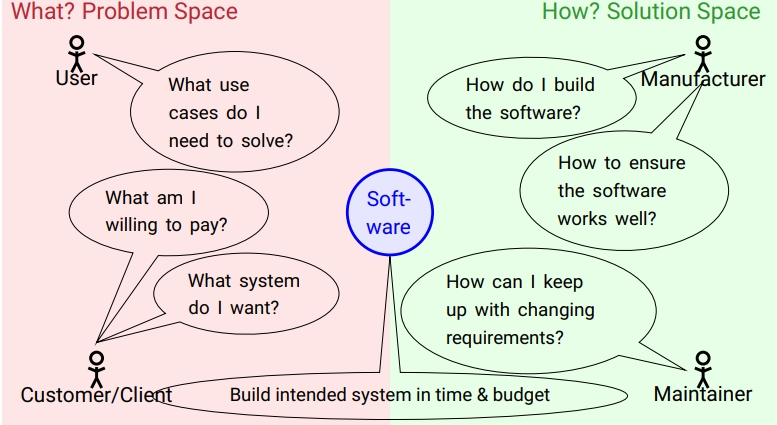
\includegraphics[width=1\textwidth]{Images/What vs How.jpeg}
\end{minipage}
\begin{minipage}{0.5\textwidth}
    \centering
    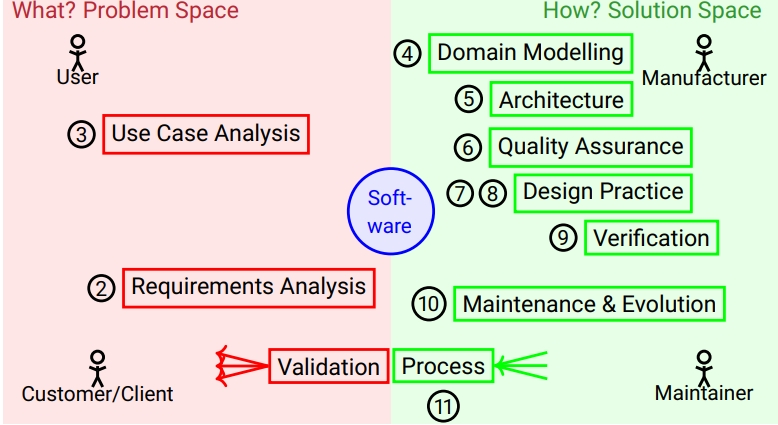
\includegraphics[width=1\textwidth]{Images/What vs How 2.jpeg}
\end{minipage}
\subsection{Software Engineering: Demarcation Lines}
\begin{infoBox}[title=Was ist Systems Engineering?]
    Systems Engineering beschäftigt sich mit der Planung, Entwicklung und Umsetzung von komplexen Systemen, die aus verschiedenen Komponenten bestehen, wie Hardware, Software, Mensch-Maschine-Schnittstellen und Betriebsprozessen. Das Ziel ist es, ein Gesamtsystem zu entwerfen, das den Anforderungen entspricht und gut funktioniert. Systems Engineering bezieht sich also auf das „große Ganze“ und umfasst alle Schritte von der Konzeptionsphase bis zur Implementierung und Wartung des Systems.
\end{infoBox}
\begin{infoBox}[title=Was ist Software Engineering?]
    Software Engineering hingegen konzentriert sich speziell auf die Entwicklung, den Betrieb und die Wartung von Software. Es ist ein Teilbereich des Systems Engineering, wenn das Gesamtsystem Software enthält oder auf Software basiert. Das Ziel ist es, Software systematisch und diszipliniert zu entwickeln, um sie zuverlässig und qualitativ hochwertig zu machen.
\end{infoBox}
\begin{defBox}[title=Systems Engineering (Systemtechnik) vs. Software Engineering]
    \begin{itemize}
        \item \red{Overall systemic} objectives and requirements
        \begin{infoBox}
            \begin{itemize}
                \item Beim Systems Engineering werden zunächste die Gesamtziele und Anforderungen des gesamten Systems definiert. Dazu gehört, festzulegen, was das System insgesamt leisten soll, welche Leistungsmerkmale es haben muss und welche Einschränkungen zu berücksichtigen sind
                \item Software Engineering fokussiert sich dann darauf, diese Anforderungen für den Softwaretiel des Systems umzusetzen
            \end{itemize}
        \end{infoBox}
        \item Assigning system functions between \red{hardware and software}
        \begin{infoBox}
            \begin{itemize}
                \item Systems Engineering befasst sich mitder Entscheidung, welche Funktionen durch Hardware und welche durch Software realisiert werden sollen. Diese Entscheidung beeinflusst die Gesamtarchitektur des Systems
                \item Software Engineering setzt diese Entscheidungen um, indem es die Software entwickelt, die die zugewiesenen Funktionen übernimmt
            \end{itemize}
        \end{infoBox}
        \item Defining interfaces between \red{hardware and software}
        \begin{infoBox}
            \begin{itemize}
                \item Systems Engineering legt die Schnittstellen zwischen den verschiedenen Systemkomponenten fest, z.B. wie Hardware und Software miteinander kommunizieren sollen
                \item Software Engineering implementiert dann diese Schnittstellen auf der Softwareseite, um sicherzustellen, dass die Software korrekt mit der Hardware interagiert
            \end{itemize}
        \end{infoBox}
        \item Full \red{system acceptance} tests
        \begin{infoBox}
            \begin{itemize}
                \item Systems Engineering umfasst umfassende Tests des gesamten Systems, um sicherzustellen, dass alle Komponenten (Hardware, Software, Mensch-Maschine-Schnittstellen usw.) nahtlos zusammenarbeiten und die definierten Anforderungen erfüllen
                \item Software Engineering führt dagegen spezifische Tests für die Software durch, um deren Funktionalität, Leistung und Qualität sicherzustellen, bevor sie in die Systemtests einfließt
            \end{itemize}
        \end{infoBox}
    \end{itemize}
    are aspects of \red{Systems Engineering}: Software Engineering is a \blue{part of} Systems Engineering (where systems are \red{software systems})
\end{defBox}
\begin{defBox}[title=Computer Science vs. Software Engineering]
    Software Engineering ist a subfield of Computer Science (at least in Europe)
\end{defBox}
\subsection{Importance of Software Production Environment}
\begin{defBox}
    Social aspects of Software Engineering: important, but beyont this course
\end{defBox}
\begin{defBox}[title=Software Development Problems caused by Environment]
    \begin{itemize}
        \item Lack of customer/user involvement:
        \begin{itemize}
            \item insufficient validation
            \item inadequate specification: incomplete, ambiguous, inconsistent
        \end{itemize}
        \item Constantly \red{changing requirements} (moving target)
        \begin{itemize}
            \item gets worse the longer it takes to ship the product
            \item (erroneous) perception: changing software is easier than hardware
        \end{itemize}
        \item Insufficient \red{training} of software engineers
        \item \red{Management} (until recently, almost no Comuper Scientists)
        \item \red{Unsuitable} (prescribed) methods, languages, tools
    \end{itemize}
\end{defBox}
\begin{infoBox}
    Die Softwareentwicklung wird stark von der Umgebung beeinflusst, in der sie stattfindet. Mangelnde Kundenbeteiligung, ständig wechselnde Anforderungen, unzureichende Schulung der Entwickler, mangelndes technisches Management und ungeeignete Methoden oder Werkzeuge können alle zu ernsthaften Problemen führen. Es ist wichtig, diese Herausforderungen zu erkennen und proaktive Maßnahmen zu ergreifen, um sicherzustellen, dass die Softwareentwicklung erfolgreich verläuft und die gewünschten Ergebnisse erzielt werden.
\end{infoBox}
\begin{defBox}[title=Detection an Error Presumes an Expectation (Requirement)]
    \begin{infoBox}
        Die Idee hier ist, dass man einen Fehler nur erkennen kann, wenn man eine Vorstellung davon hat, was korrekt oder erwatungsgemäß sein sollte. Diese Vorstellung wird durch die Anforderungen definiert
        \begin{itemize}
            \item \fatsf{Anforderungen als Maßstab:} Anforderungen dienen als Maßstab für das , was die Software tun sollte. Wenn ein Programm funktioniert, wie es soll, und die Erwartungen erfüllt, gehen wir davon aus, dass es keine Fehler gibt
        \end{itemize}
    \end{infoBox}
    \begin{itemize}
        \item Few errors are \enquote{obvious} (such as a crash)
        \begin{infoBox}
            \begin{itemize}
                \item \fatsf{Offensichtliche Fehler:} Einige Fehler sind sofort erkennbar, wie ein Programm, das abstürzt. Solche Fehler sind leicht zu identifizieren und zu beheben, weil sie sofortige Auswirkungen auf die Benutzer haben
                \item \fatsf{Stille Fehler:} Viele Fehler sind jedoch nicht sofort offensichtlich und können lange unentdeckt bleiben. Zum Beispiel:
                \begin{itemize}
                    \item \fatsf{Falsches Ergebnis einer komplexen Berechnung:} Wenn ein Programm falsche Ergebnisse liefert, ohne dass es abstürzt oder eine Fehlermeldung ausgibt, kann es lange dauern, bis dieser Fehler erkannt wird
                \end{itemize}
            \end{itemize}
        \end{infoBox}
        \item Without precise \red{requirements} threre are no \red{errors}:\\
        INABIAF - \enquote{It´s not a bug, it´s a feature}
        \begin{infoBox}
            Wenn die Anforderungen unklar, unvollständig oder mehrdeutig sind, ist es schwierig, einen Fehler zu definieren. In solchen Fällen kann eine Abweichung von einer ungenauen Anforderung nicht wirklich als Fehler betrachtet werden, da es nicht klar ist, was die Software leisten sollte.
            \begin{itemize}
                \item \fatsf{INABIAF:} Das Akronym steht für \enquote{It´s Not a Bug, It´s a Feature} und beschreibt die Haltung, dass eine unerwartete Verhaltensweise als gewollte Funktion angesehen werden kann, wenn die Anforderungen nicht klar definiert sind. Dies kaann zu Verwirrung und Frustration bei Benutzern führen 
            \end{itemize}
        \end{infoBox}
        \item Many errors traceable to \blue{VVD}: \red{Validation, Verifikation, Documentation}
    \end{itemize}
    $\Rightarrow$ \blue{Insufficient match between requirements and realization}
\end{defBox}
\begin{defBox}
    Error in design/code $\subsetneq$ Software \red{construction} error 
\end{defBox}
\begin{defBox}[title=\enquote{Software} Errors present in every Construction Phase]
    \begin{itemize}
        \item Requirements analysis:
        \begin{itemize}
            \item Unanticipated requirements
            \item Silently changed requirements
        \end{itemize}
        \item Use case analysis
        \item Domain modelling      \item Verification 
        \item Design                \item Validation 
        \item Algorithms            \item Documentation
        \item Coding                \item Maintenance
    \end{itemize}
\end{defBox}
\subsection{Take-home Message:}
\begin{defBox}
    Software development must be economical
\end{defBox}
\begin{defBox}
    Software development must be safe and ensure high quality
\end{defBox}
\begin{defBox}
    Software development must follow scientific \& engineering principles
\end{defBox}

\clearpage
\section{Requirements Engineering}
\subsection{The CaSh Case Study}
\begin{figure}[h]
    \centering
    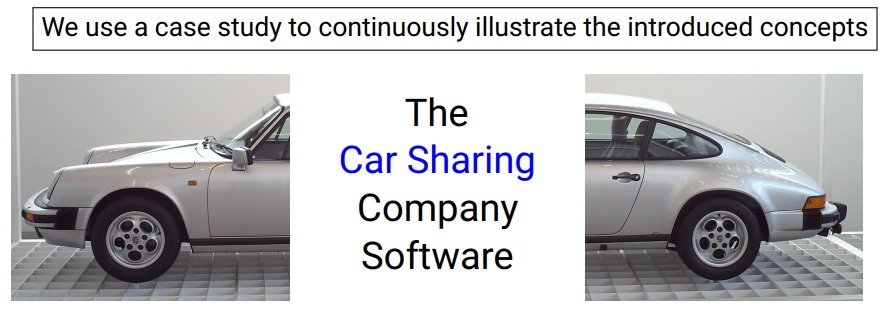
\includegraphics[width=1\textwidth]{Images/The CaSh Case Study.jpeg}
\end{figure}

\subsubsection*{Description}
\begin{defBox}[title=Main Roles \& Functionalities]
	\begin{itemize}
		\item Role-independent
		\begin{itemize}
			\item Authentication
		\end{itemize}
		\item Administrator
		\begin{itemize}
			\item Add/change new cars, rental locations
			\item Billing
		\end{itemize}
		\item User
		\begin{itemize}
			\item Check availability
			\item Request booking
			\item Change booking
		\end{itemize}
		\item Service Staff
		\begin{itemize}
			\item Take out vehicle for service 
		\end{itemize}
	\end{itemize}
\end{defBox}

\clearpage
\subsubsection*{Provision of services for different actors}
\begin{figure}[h]
    \centering
    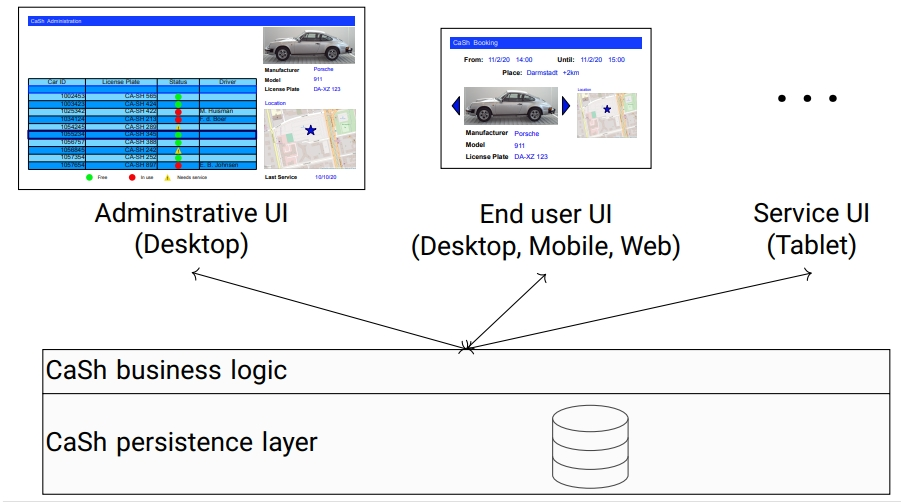
\includegraphics[width=0.87\textwidth]{Images/Provision of services for different actors.jpeg}
\end{figure}

\subsubsection*{Requirements Engineering}
\begin{figure}[h]
    \centering
    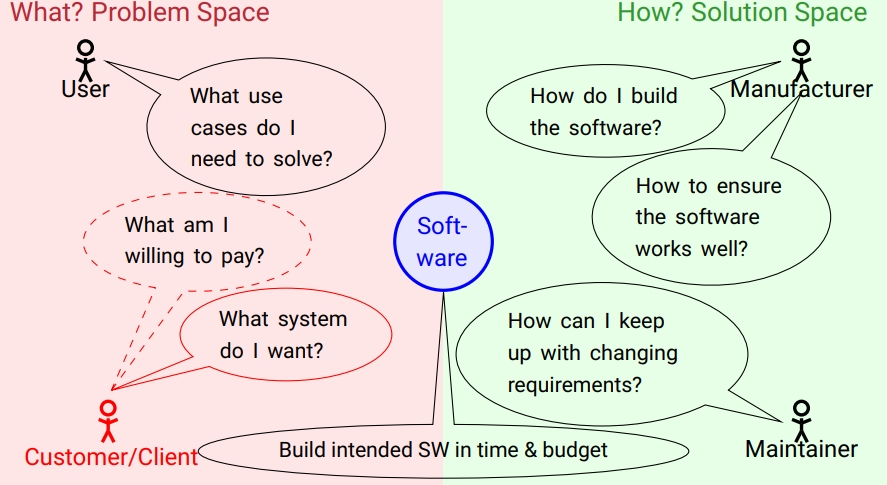
\includegraphics[width=0.87\textwidth]{Images/Requirements Engineering.jpeg}
\end{figure}

\clearpage
\subsection*{Requirements Engineering}
\blue{Assume:} You are contracted by \red{client} to develop CaSh
\begin{defBox}
	Systematic approach to the question: \red{What} has to be developed?
\end{defBox}
\begin{itemize}
	\item Understanding the problems in requirements elicitation 
	\item Different kinds of requirements
	\item Requirement engineering workflow
	\item Modelling requirements (next lecture)
	\begin{itemize}
		\item Scenarios \& Use cases
		\item Notations: Textual \& Graphical
	\end{itemize}
\end{itemize}

\subsection{Why Requirements Analysis is Difficult}
Mary had a little lamb.\\
What does the sentence mean?
\begin{defBox}[title=Meanings of to have]
	\begin{enumerate}
		\item to hold in possession as a property
		\item to trick or fool someone (been had by a someone)
		\item to beget or bear (habe a baby)
		\item to partake (have as a meal)
		\item ...
	\end{enumerate}
\end{defBox}
\begin{defBox}[title=Meanings of lamb]
	\begin{enumerate}
		\item a young sheep less than one year
		\item the young of various other animals (antelope, etc.)
		\item a person as gentle or weak as a lamb
		\item a person easily cheated or deceived
		\item the flesh of lamb used as food
		\item ...
	\end{enumerate}
\end{defBox}
Mary hd a little lamb\\
What does the sentence mean?
\blue{Possible Meanings:}
\begin{itemize}
	\item Mary owned once a lamb under one year
	\item Mary gave birth to an antelope
	\item ...
\end{itemize}
\begin{infoBox}
    Zusammengefasst verdeutlicht diese Beispiele, dass Sprache oft mehrdeutig ist, und genau diese Mehrdeutigkeit macht es im Requirements Engineering schwer, präzise Anforderungen zu spezifizieren.
\end{infoBox}

\subsection*{Application to Case Study?}
\begin{defBox}[title=What is meant with ...?] 
	\begin{itemize}
		\item \enquote{The status of a car is \red{in use}, \red{free} or \red{need service}.}
		\item \enquote{Each car must have a unique license plate number.}\\
		What if the care has not yet been registered?
		\item \enquote{Das System muss sicher sein.}\\
		\enquote{\red{sicher}} in welchem Sinne? secure or safe?
		\item Exercise: find ambiguous specifications in an API of your choice
	\end{itemize}
\end{defBox}

\subsection{What are Requirements?}
\begin{defBox}[title=Definition(Requirements)]
	Requirements are the descriptions of 
	\begin{itemize}
		\item the \red{services provided by the system} and
        \begin{infoBox}
            Den Dienstleistungen oder Funktionen, die das System bereitstellen soll.
            \begin{itemize}
                \item Zum Beispiel: Ein Online-Shop sollte es Benutzern ermöglichen, Produkte zu suchen, in den Warenkorb zu legen und zu bezahlen.
            \end{itemize}
        \end{infoBox}
		\item the \red{operational constraints}
        \begin{infoBox}
            Den betrieblichen Einschränkungen oder Rahmenbedingungen, unter denen das System arbeitet
            \begin{itemize}
                \item Zum Beispiel: Das System muss mindestens 100 Datenbankabfragen pro Sekunde verarbeiten können (Datenbank-Durchsatz).
                \item Weitere Beispiele sind Anforderungen an den Speicherbedarf des Systems oder an unterstützte Navigationssysteme (z.B. GPS, Galileo, GLONASS).
            \end{itemize}
        \end{infoBox}
	\end{itemize}
\end{defBox}
\begin{defBox}
	\begin{itemize}
		\item Database throughput (number of database queries per second)
		\item System memory
		\item Navigation systems GPS, Galileo, GLONASS
		\item ...
	\end{itemize}
\end{defBox}

\clearpage
Requirements are written down
\begin{itemize}
	\item in the \red{System Requirements Specification} (SRS) Document (German: Pflichtenheft)
	\item as \red{user stories}, structured natural language, use cases, state diagrams, ... and stored in the \red{product backlog} (ordered list of requirements)
\end{itemize}
\begin{infoBox}
    \fatsf{Wie werden Anforderungen dokumentiert?}\\
    \begin{enumerate}
        \item \fatsf{System Requirements Specification (SRS)}, auf Deutsch oft als \fatsf{Pflichtenheft} bezeichnet.
        \begin{itemize}
            \item Das SRS ist ein strukruriertes Dokument, das alle Anforderungen an das System detailliert beschreibt.
            \item Es ist die Grundlage für die Entwicklung und dient als Referenz für die Überprüfung, ob die Anforderungen erfüllt wurden
        \end{itemize}
        \item \fatsf{Andere Darstellungsformen von Anforderungen:}
        \begin{itemize}
            \item \fatsf{User Stories:} Kurze, informelle Beschreibungen aus der Perspektive eines Benutzers. Beispiel: \enquote{Als Benutzer möchte ich nach Produkten suchen können, um das passende Angebot zu finden.}
            \item \fatsf{Strukturiertes natürliches Englisch:} Eine präzise, aber leicht verständliche Form der Beschreibung.
            \item \fatsf{Use Cases:} Szenarien, die beschreiben, wie Bunutzer das System in verschiedenen Situationen nutzen.
            \item \fatsf{Zustandsdigramme:} Grafische Darstellungen der Zustände eines Systems und deren Übergänge.
        \end{itemize}
        \item \fatsf{Product Backlog:} Eine geordnete Liste der Anforderungen.
        \begin{itemize}
            \item Im agilen Entwicklungsansatz (z.B. Scrum) werden Anforderungen im Product Backlog gesammelt und priorisiert.
            \item Das Backlog ist dynamisch, d.h., es wird im Laufe des Projekts immer wieder aktualisiert.
        \end{itemize}
    \end{enumerate}
\end{infoBox}
\begin{defBox}
	Requirements are \red{not} solutions
\end{defBox}
\begin{infoBox}
    \begin{itemize}
        \item Anforderungen beschreiben, \fatsf{was} das System tun soll oder \fatsf{unter welchen Bedingungen} es arbeiten soll, aber nicht \fatsf{wie} es das erreichen soll.
        \item z.B.: Eine Anforderung könnte sein, dass die Suchfunktion innerhalb von 2 Sekunden Ergebnisse liefern muss. Diese Anforderung sagt nichts darüber aus, wie diese Geschwindigkeit technisch erreicht wird.
    \end{itemize}
\end{infoBox}
\subsection{Requirement Types}
\begin{defBox}[title=Many Different Types of Requirements]
	\begin{itemize}
		\item \red{User} requirements
		\item \red{System} requirements
		\item \red{Functional} requirements
		\item \red{Non-functional} requirements
		\item \red{Domain} requirements
	\end{itemize}
	\blue{Let's discuss them in turn}
\end{defBox}
\subsubsection{User Requirements}
\begin{defBox}[title=User Requirements]
	State in natural language and (semi-formal) diagrams:
	\begin{itemize}
		\item What are the \red{services} expected to be provided by the system
		\item What are the \red{operational constraints} (Betriebsparameter)
	\end{itemize}
	Often high-level and abstract descriptions (normally \red{written by the customer})
\end{defBox}
\begin{infoBox}
    Benutzeranforderungen (User Requirements) sind Anforderungen, die aus der Perspektive der Benutzer oder Kunden beschrieben werden. Sie geben an, \fatsf{welche Dienste das System bereitstellen soll} und \fatsf{welche Betriebsparameter oder Einschränkungen} dabei gelten. Benutzeranforderungen sind oft \fatsf{hochgradig, abstrakt und allgemein formuliert}, um die grundlegenden Erwartungen an das System auszudrücken. Normalerweise werden sie vom Kunden oder den Stakeholdern verfasst.\\
    \fatsf{Merkmale von Benutzeranforderungen:}
    \begin{enumerate}
        \item \fatsf{Formulierung in natürlicher Sprache und Diagrammen:}
        \begin{itemize}
            \item Benutzeranforderungen werden oft in \fatsf{natürlicher Sprache} beschrieben, damit sie für alle Beteiligten (einschließlich Kunden und Entwickler) verständlich sind.
            \item \fatsf{Semi-formale Diagramme} wie Use-Case-Diagramme oder einfache Ablaufdiagramme können verwendet werden, um die Anforderungen graphisch darzustellen und besser zu veranschaulichen.
        \end{itemize}
        \item \fatsf{Beschreiben der erwarteten Dienste des Systems:}
        \begin{itemize}
            \item Es wird festgelegt, \fatsf{welche Funktionalitäten} oder \fatsf{Dienste} das System bereitstellen soll, ohne dabei zu sehr ins Detail zu gehen, wie diese technisch umgesetzt werden.
            \item Beispiel: \enquote{Das System soll es Benutzern ermöglichen, Flugtickets online zu buchen.}
        \end{itemize}
        \item \fatsf{Definieren von Betriebsparametern (operational contraints)}
        \begin{itemize}
            \item Benutzeranforderungen enthalten auch \fatsf{Rahmenbedingungen}, unter denen das System funktionieren soll, z.B. gesetzliche Vorgaben, Leistungsanforderungen oder bestimmte Betriebsumgebungen.
            \item Beispiel: \enquote{Das System muss den deutschen Datenschutzbestimmungen entsprechen}
        \end{itemize}
    \end{enumerate}
\end{infoBox}
\begin{defBox}[title=Example]
	\enquote{CaSh shall keep track of all bookings as required by German law} (e.g., in case of speeding tickets, for tax purposes)
\end{defBox}
\begin{infoBox}
    \fatsf{CaSh soll alle Buchungen gemäß den Anforderungen des deutschen Rechts nachverfolgen (z.B. Geschwindigkeitsverstöße oder steuerliche Zwecke)}\\
    Die Anforderung drückt aus, dass das System \fatsf{alle Buchungen aufzeichnen und verwalten soll}, um den gesetzlichen Anforderungen gerecht zu werden. Es wird jedoch \fatsf{nicht spezifiziert}, wie das System dies technisch tun soll oder welche Datenbanktechnologien verwendet werden sollen. Es bleibt auf einer \fatsf{hohen, abstrakten Ebene.}
\end{infoBox}

\clearpage
\subsubsection{System Requirements}
\begin{defBox}[title=System Requirements (Systemanforderungen)]
	\red{Precise and detailed} specification of the system's
	\begin{itemize}
		\item functions, services and
		\item operational constraints
	\end{itemize}
\end{defBox}
\begin{infoBox}
    Systemanforderungen (System Requirements) sind \fatsf{präzise und detaillierte Spezifikationen} darüber, was ein System leisten soll. Sie bauen auf den Benutzeranforderungen auf, sind jedoch genauer und technischer. Systemanforderungen legen fest, \fatsf{welche Funktionen und Dienstleistungen} das System bereitstellen muss und \fatsf{unter welchen Betriebsbedingungen} es funktionieren soll.
\end{infoBox}
\begin{defBox}[title=Example (CaSh System Requirements)]
    \begin{itemize}
        \item \enquote{Upon successful completion of a booking, the user must be shown an overview of the booking details.}
        \item \enquote{Booking details must be stored by CaSh for 10 years from the booking date onwards.}
        \item \enquote{Booking details consist of pickup and return date, care details (license plate number, ...), user name + address and payment information.}
    \end{itemize}
\end{defBox}
\begin{infoBox}
    \begin{enumerate}
        \item \enquote{Nach erfolgreichem Abschluss einer Buchung muss dem Benutzer eine Übersicht der Buchungsdetails angezeigt werden.}
        \item \enquote{Buchungsdetails müssen von CaSh für 10 Jahre ab dem Buchungsdatum gespeichert werden.}
        \item \enquote{Buchungsdetails bestehen aus Abhol- und Rückgabedatum, Fahrzeugdetails (z.B. Kennzeichnen), Benutzername, Adresse und Zahlungsinformationen.}
    \end{enumerate}
\end{infoBox}

\clearpage
\begin{defBox}[title=Characteristics of system requirements:]
    \begin{itemize}
        \item \red{Refinement} of user requirements
        \item Determine the \red{system interface} (functional, \red{not} technical interface) $\implies$ Define \red{solution space}
        \item Recorded as part of the \red{system requirements document} (functional specification) and typically part of the contract with client
        \item Authored by \red{software developer} or \red{business analyst} in collaboration with \red{client}
        \item (Dt.: Grundlage für das Pflichtenheft)
    \end{itemize}
\end{defBox}
\begin{infoBox}
    \fatsf{Merkmale der Systemanforderungen:}
    \begin{enumerate}
        \item \fatsf{Verfeinerung der Benutzeranforderungen}
        \begin{itemize}
            \item Während Benutzeranforderungen \fatsf{allgemein} formuliert sind, werden sie durch die Systemanforderungen in \fatsf{spezifische und messbare Anforderungen} übersetzt.
            \item Sie konkretisieren, \fatsf{wie die in den Benutzeranforderungen beschriebenen Erwartungen erfüllt werden sollen.}
        \end{itemize}
        \item \fatsf{Definition der Systemschnittstellen:}
        \begin{itemize}
            \item Systemanforderungen legen fest, \fatsf{wie das System mit anderen Systemen, Benutzern oder Geräten interagiert,} ohne jedoch die genauen technischen Implementierungsdetails anzugeben.
            \item Es wird der \fatsf{Lösungsraum} definiert, d.h., welche Ansätze oder Technologien zur Erfüllung der Anforderungen verwendet werden können
        \end{itemize}
        \item \fatsf{Teil der Systemanforderungsdokumentation:}
        \begin{itemize}
            \item Die Anforderungen werden im \fatsf{System Requirements Specification (SRS)} festgehalten, das häufig auch als \fatsf{Pflichtenheft} bezeichnet wird.
            \item Das SRS-Dokument ist oft ein \fatsf{Bestandteil des Vertrags} zwischen dem Kunden und dem Entwickler, da es genau beschreibt, was geliefert werden muss.
        \end{itemize}
        \item \fatsf{Erarbeitet durch Entwickler oder Business Analysten in Zusammenarbeit mit dem Kunden:}
        \begin{itemize}
            \item Systemanforderungen werden typischerweise von \fatsf{Softwareentwicklern oder Business-Analysten} verfasst, die eng mit dem Kunden zusammenarbeiten, um sicherzustellen, dass die Spezifikationen den Anforderungen und Erwartungen entsprechen.
        \end{itemize}
    \end{enumerate}
\end{infoBox}
\subsubsection{Functional Requirements}
\begin{defBox}[title=Functional requirement ($\neq$ functional specification)]
    Functionality that is clearly identifiable and localized in the \red{code}
\end{defBox}
\begin{infoBox}
    Funktionale Anforderungen sind spezifische Beschreibungen von \fatsf{Funktionen oder Dienstleistungen,} die ein System bereitstellen soll. Sie geben an, \fatsf{was das System tun soll,} ohne dabei zu beschreiben, \fatsf{wie} es technisch umgesetzt wird. Funktionale Anforderungen sind \fatsf{direkt im Code nachvollziehbar}, da sie sich auf klare definierte Funktionen beziehen, die im System implementiert werden.
\end{infoBox}
\begin{defBox}[title=Functional Requirements Specify ...]
    \begin{itemize}
        \item Services to be provided by the system, for instance:
        \begin{itemize}
            \item Authentication
            \item Querying for available cars
            \item Sending confirmation emails
        \end{itemize}
        \item \red{System reactions} to specific inputs/events, for instance:
        \begin{itemize}
            \item Error message when selected return date is before pick up date
        \end{itemize}
        \item \red{System behavior} in specific situations, for instance:
        \begin{itemize}
            \item Network disruption during booking process
        \end{itemize}
    \end{itemize}
\end{defBox}
\begin{infoBox}[title=Was spezifizieren funktionale Anforderungen]
    Funktionale Anforderungen legen fest, welche \fatsf{Dienstleistungen, Systemreaktionen und Systemverhalten} in bestimmten Situationen das System bieten soll:
    \begin{enumerate}
        \item \fatsf{Dienste, die vom System bereitgestellt werden:}
        \begin{itemize}
            \item Diese Anforderungen beschreiben, \fatsf{welche spezifischen Funktionen das System bieten soll.}
            \item Beispiele:
            \begin{itemize}
                \item \fatsf{Authentifizierung:} Das System muss es Benutzern ermöglichen, sich mit Benutzernamen und Passwort anzumelden.
                \item \fatsf{Abfragen nach verfügbaren Autos}
                \item \fatsf{Versenden von Bestätigungs-E-Mails} 
            \end{itemize}
        \end{itemize}
        \item \fatsf{Systemreaktionen auf bestimmte Eingaben oder Ereignisse:}
        \begin{itemize}
            \item Funktionale Anforderungen geben an, \fatsf{wie das System auf bestimmte Benutzeraktionen oder Ereignisse reagieren soll.}
            \item Beispiel: \fatsf{Fehlermeldung bei ungültigen Eingaben:} Wenn das Rückgabedatum vor dem Abholdatum liegt, muss das System eine Fehlermeldung anzeigen.
        \end{itemize}
        \item \fatsf{Systemverhalten in spezifischen Situationen:}
        \begin{itemize}
            \item Sie spezifizieren, \fatsf{wie das System sich in bestimmten Ausnahmefällen oder besonderen Umständen verhalten soll.}
            \item Beispiel: \fatsf{Netzwerkunterbrechung während des Buchungsvorgangs:} Das System muss in der Lage sein, den Buchungsvorgang bei einer Netzwerkunterbrechung wiederaufzunehmen oder die Benutzer entsprechend zu informieren.
        \end{itemize}
    \end{enumerate}
\end{infoBox}
\begin{infoBox}[title=Unterschied zu einer funktionalen Spezifikationen]
    \begin{itemize}
        \item \fatsf{Funktionale Anforderungen} beschreiben \fatsf{was} das System leisten soll (z.B. bestimmte Funktionen, Dienste oder Reaktionen), während eine \fatsf{funktionale Spezifikation} detailliert beschreibt, \fatsf{wie} diese Anforderungen technisch umgesetzt werden sollen.
        \item Beispiel: Eine funktionale Anforderung könnte sein, dass Benutzer sich anmelden können, während die funktionale Spezifikation festlegt, welche Verschlüsselungsprotokolle und Sicherheitsmechanismen für die Anmeldung verwendet werden.
    \end{itemize}
\end{infoBox}
\subsubsection{Non-Functional Requirements}
\begin{defBox}[title=Non-functional Requirements (NFR)]
    Constraints on the services or functions offered by the system, including:
    \begin{itemize}
        \item Service level agreement (SLA)
        \item Constraints from development process (sequential/incremental)
        \item Alignment to standards (for example, protocols)
    \end{itemize}
\end{defBox}
\begin{infoBox}
    Nicht-funktionale Anforderungen (Non-functional Requirements, NFR) beschreiben \fatsf{Einschränkungen oder Rahmenbedingungen}, unter denen die Funktionen eines Systems bereitgestellt werden müssen. Sie betreffen die \fatsf{Qualitätsmerkmale} des Systems und beziehen sich auf \fatsf{Leistung, Sicherheit, Benutzerfreudlichkeit, Zuverlässigkeit} usw., anstatt auf spezifische Funktionen.
\end{infoBox}
\begin{defBox}
    NFRs are often cross-cutting concerns that apply to the whole system
\end{defBox}
Meeting such requirements is usually impossible by adding a piece of code at a specific location or cannot be guranteed by software alone.
\begin{infoBox}[title=Merkmale nicht-funktionaler Anforderungen]
    \begin{enumerate}
        \item \fatsf{Oft systemübergreifende Anforderungen:}
        \begin{itemize}
            \item Sie sind \fatsf{querschnittliche Anforderungen}, die für mehrere oder alle Teile des Systems gelten, wie z.B. Sicherheitsstandards oder Antwortzeiten.
        \end{itemize}
        \item \fatsf{Schwer durch einfache Code-Änderungen zu erfüllen:}
        \begin{itemize}
            \item Es ist oft \fatsf{nicht möglich, eine nicht-funktionale Anforderung durch Hinzufügen von Code an einer bestimmten Stelle zu erfüllen.} Sie erfordern meist \fatsf{übergreifende Maßnahmen im gesamten System.}
            \item Zum Beispiel ist es nicht genug, nur an einer Stelle im Code Änderungen vorzunehmen, um die \fatsf{Gesamtleistung oder Sicherheit} des Systems sicherzustellen.
        \end{itemize}
    \end{enumerate}
\end{infoBox}

\begin{defBox}[title=Example (CaSh non-functional requirements)]
    \begin{itemize}
        \item The database must be able to process 1000 queries (Abfragen) per second
        \begin{infoBox}
            Diese Anforderung betrifft die \fatsf{Leistungsfähigkeit} des Systems.
        \end{infoBox}
        \item User data must only be accessible to authorized persons
        \begin{infoBox}
            Diese Anforderung bezieht sich auf die \fatsf{Sicherheit und Datenschutz} im System.
        \end{infoBox}
        \item The software development model must be CMMI Level 4 certified
        \begin{infoBox}
            \textbf{Diese Anforderung beschreibt eine \fatsf{Prozessanforderung} und legt fest, welches Entwicklungsmodell verwendet werden soll.}
        \end{infoBox}
        \item CaSh must provide the booking data for the accounting system (Buchhaltungssystem)
        \begin{infoBox}
            Diese Anforderung betrifft die \fatsf{Interoperabilität}, also die Fähigkeit des Systems, mit anderen Systemen zusammenzuarbeiten.
        \end{infoBox}
    \end{itemize}
\end{defBox}

\clearpage
\begin{defBox}[title=Non-functional requirements]
    \begin{enumerate}
        \item \red{Product requirements}
        \begin{itemize}
            \item Reliability, availability
            \item Effeciency (performance, memory)
            \item Usability
            \item Portability
        \end{itemize}
        \item \red{Organisational requirements}
        \begin{itemize}
            \item Delivery mode (beta, continuous, ...)
            \item Implementation (programming language, frameworks, ...)
            \item Standardization (ISO 9000, CMMI, ...)
        \end{itemize}
        \item \red{External requirements}
        \begin{itemize}
            \item Interoperability (TUCaN-Moodle)
            \item Ethical aspects
            \item Legal aspects (safety, security, privacy, ...)
        \end{itemize}
    \end{enumerate}
\end{defBox}
\begin{infoBox}[title=Arten von nicht-funktionalen Anforderungen:]
    \begin{enumerate}
        \item \fatsf{Produktanforderungen:}
        \begin{itemize}
            \item Betreffen die \fatsf{Eigenschaften des Produkts}, wie \fatsf{Zuverlässigkeit, Verfügbarkeit, Effizienz, Benutzerfreundlichkeit und Portabilität.}
            \item Beispiel: \enquote{Die Software muss in weniger als 2 Sekunden auf eine Benutzeranfrage reagieren.}
        \end{itemize}
        \item \fatsf{Organisatorische Anforderungen:}
        \begin{itemize}
            \item Beziehen sich auf \fatsf{organisatorische Rahmenbedingungen}, wie \fatsf{Liefermode, Entwicklungsprozesse, Standards und Zertifizierungen}
            \item Beispiel: \enquote{Die Software muss nach ISO 9000 zuertifiziert sein.}
        \end{itemize}
        \item \fatsf{Externe Anforderungen:}
        \begin{itemize}
            \item Beziehen sich auf \fatsf{gesetzliche, ethische oder externe technische Anforderungen}, wie \fatsf{Datenschutzgesetze, Sicherheitsvorschriften oder Interoperabilität mit anderen Systemen.}
            \item Beispiel: \enquote{Die Software muss die Datenschutz-Grundverordnung (DSGVO) einhalten.}
        \end{itemize}
    \end{enumerate}
\end{infoBox}

\clearpage
\subsubsection{Functional vs. Non-Functional Requirements}
\begin{defBox}[title=Observations]
    Non-functional requirements ...
    \begin{itemize}
        \item may result in the identification of functional requirements
        \item are often more mission-critical than individual functional requirements
    \end{itemize}
\end{defBox}
\begin{defBox}[title=Example (Relative importance of non-functional requirements)]
    A car shring system that does not support to confirm a booking by email is still usable; if the system is not secure or reliable, it is worthless.
\end{defBox}
\begin{infoBox}[title=Beobachtungen zum Unterschied:]
    \begin{itemize}
        \item \fatsf{Nicht-funktionale Anforderungen können funktionale Anforderungen identifizieren:}
        \begin{itemize}
            \item Wenn zum Beispiel eine nicht-funktionale Anforderung lautet, dass das System \fatsf{sicher sein muss}, kann daraus eine funktionale Anforderung entstehen, wie das \fatsf{Implementieren von Benutzerzugriffsrechten oder einer Zwei-Faktor-Authentifizierung.}
            
        \end{itemize}
        \item \fatsf{Nicht-funktionale Anforderungen sind oft kritischer für das Gesamtsystem:}
        \begin{itemize}
            \item Während ein System möglicherweise ohne bestimmte \fatsf{funktionale Anforderungen} noch funktionieren kann (z.B. das Versenden von E-Mails), könnte es \fatsf{unbrauchbar sein}, wenn es die \fatsf{nicht-funktionalen Anforderungen} wie \fatsf{Sicherheit, Zuverlässigkeit oder Leistung} nicht erfüllt.
            \item \fatsf{Beispiel:} Ein Carshring-System, das keine Buchungsbestätigung per E-Mail senden kann, ist immer noch nutzbar. Wenn das System jedoch \fatsf{unsicher oder unzuverlässig} ist, verliert es seinen Wert, da Benutzer ihm nicht vertrauen würden und es nicht zuverlässig genutzt werden kann.
        \end{itemize}
    \end{itemize}
\end{infoBox}

\subsubsection{Ensuring Verifiability of Non-Functional Requirements}
How to ckeck whether non-functional requirements are met?
\begin{defBox}[title=Example (Typical usability requirement)]
    \enquote{The user interface should be easy to use.}
\end{defBox}
\begin{defBox}[title=Problems with this Requirement]
    \begin{itemize}
        \item How to measure \enquote{easy}?
        \item Easy for \red{whom}?
        \begin{itemize}
            \item Expert user
            \item Average user
            \item Persons with a handicap (accessiblity)
        \end{itemize}
    \end{itemize}
\end{defBox}
\begin{infoBox}
    \fatsf{\enquote{Die Benutzeroberfläche sollte leicht zu bedienen sein.}} Diese Anforderung ist subjektiv und schwer messbar. Daher wird sie in konkrete Anforderungen umgewandelt:
\end{infoBox}
\begin{defBox}[title=Concretise Formulation into Quantifiable Requirements]
    \begin{itemize}
        \item \enquote{\red{Agents} can assist in bookings and manage the car pool after one day of training}
        \item \enquote{An average \red{end user} can complete a booking in less than 5 minutes}
        \item \enquote{The user interface has scalable fonts and pop-up help text}
    \end{itemize}
\end{defBox}

\subsubsection{Domain Requirements}
\begin{infoBox}
    Domänenanforderungen sind Anforderungen, die aus der \fatsf{spezifischen Anwendungsdomäne} eines Systems abgeleitet werden, anstatt direkt aus den Bedürfnissen der Benutzer. Sie beziehen sich auf \fatsf{Regeln, Vorschriften, Standards oder Prozesse}, die für eine bestimmte Branche oder Anwendung typisch sind.
\end{infoBox}
\begin{defBox}[title=Domain Requirements]
    Derived from \red{application domain} rather than from the needs of the needs of the user
    \begin{itemize}
        \item Expressed in \red{damain-specific language} and hard to understand by software engineers
        \item Often \red{implicitly assumed} as obvious to domain experts
        \item Functional or non-functional
    \end{itemize}
\end{defBox}
\begin{defBox}[title=Example]
    Car sharing companies are required to check that new customers have a driving licence.
\end{defBox}
\begin{infoBox}[title=Merkmale von Domänenanforderungen:]
    \begin{enumerate}
        \item \fatsf{Ausgedrückt in domänenspezifischer Sprache:}
        \begin{itemize}
            \item Domänenanforderungen werden häufig in einer Sprache formuliert, die \fatsf{für Domänenexperten verständlich} ist, aber \fatsf{für Softwareingenieure schwer zu verstehen} sein kann.
            \item Das bedeutet, dass sie \fatsf{technische Begriffe oder Fachjargon} aus der betreffenden Branche enthlaten können.
        \end{itemize}
        \item \fatsf{Häufig als selbstverständlich vorausgesetzt:}
        \begin{itemize}
            \item Domänenexperten nehmen oft an, dass diese Anforderungen \fatsf{offensichtlich} und für jeden verständlich sind, was dazu führen kann, dass sie \fatsf{nicht explizit dokumentiert} werden.
            \item Dies kann zu \fatsf{Missverständnisse oder fehlenden Anforderungen} führen, wenn sie nicht korrekt an das Softwareentwicklungsteam kommuniziert werden.
        \end{itemize}
        \item \fatsf{Können funktional oder nicht-funktional sein:}
        \begin{itemize}
            \item \fatsf{Funktionale Domänenanforderungen} beziehen sich auf bestimmte Funktionen, die das System ausführen muss, um den Anforderungen der Domäne zu entsprechen.
            \item \fatsf{Nicht-Funktionale Domänenanforderungen} können Einschränkungen oder Qualitätsmerkmale betreffen, die für die Domäne wichtig sind.
        \end{itemize}
    \end{enumerate}
\end{infoBox}
\begin{infoBox}[title=Warum sind Domänenanforderungen wichtig?]
    \begin{itemize}
        \item \fatsf{Domänenanforderungen stellen sicher, dass das System den spezifischen Anforderungen der Branche entspricht}, einschließlich rechtlicher, geschäftlicher und technischer Standards.
        \item Wenn Domänenanforderungen \fatsf{nicht korrekt erfasst oder verstanden} werden, kann es zu \fatsf{schwerwiegenden Problemen} kommen, z.B. dass das System \fatsf{gesetzliche Vorschriften nicht erfüllt.}
    \end{itemize}
\end{infoBox}

\subsubsection*{How to come Up with Requirements? Requirements Engineering Process}
\begin{defBox}[title=Requirements Engineering (RE)]
    Requirements engineering is the process of
    \begin{itemize}
        \item finding,
        \item analyzing,
        \item documenting, and
        \item validating
    \end{itemize}
    software requirements
\end{defBox}
The \red{system requirements document} is created and maintained during RE

\subsection{Requirements Engineering Process-Flow}
\begin{figure}[h]
    \centering
    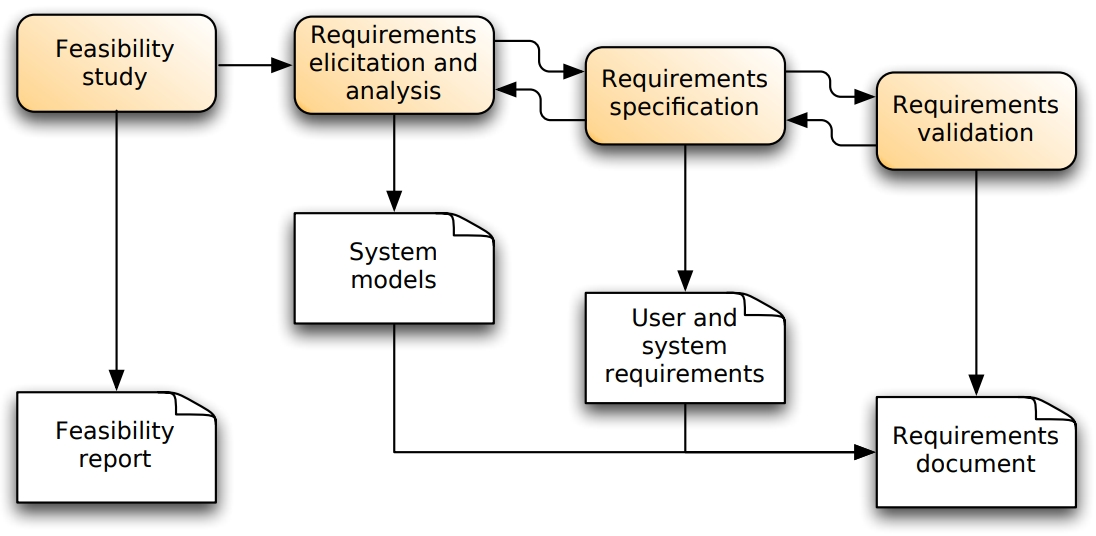
\includegraphics[width=1\textwidth]{Images/Requirements Engineering Process.jpeg}
\end{figure}

\clearpage
\subsection{RE Process}
\subsubsection*{Feasibility Study (Machbarkeitsstudie)}
\begin{infoBox}
    Die \fatsf{Machbarkeitsstudie} ist ein wichtiger Schritt im \fatsf{Requirements Engineering (RE)-Prozess} und dient dazu, eine fundierte Entscheidung darüber zu treffen, ob der \fatsf{Systementwicklungsprozess} begonnen oder fortgesetzt werden sollte. Sie hilft dabei, \fatsf{potenzielle Risiken und Herausforderungen} frühzeitig zu erkennen und abzuwägen, ob es sinnvoll ist, ein Projekt weiterzuverfolgen.
\end{infoBox}
\begin{defBox}[title=Objective of the Feasibility Study]
    Obtain a justified recommendation whether the requirements engineering and system development process should be \red{started} (or continued) based on:
    \begin{itemize}
        \item Preliminary business requirements (Vorläufige Geschäftsanforderungen)
        \begin{infoBox}
            Beschreibt die übergeordneten Ziele und Erwartungen, die das system erfüllen soll.
        \end{infoBox}
        \item Outline description of the system (Übersichtsbeschreibung des Systems)
        \begin{infoBox}
            Eine allgemeine Darstellung, wie das System funktionieren soll und welche Hauptfunktionen es bietet.
        \end{infoBox}
        \item Description of how the system is intended to support business processes (Beschreibung der Unterstützung von Geschäftsprozessen)
        \begin{infoBox}
            Erklärt, wie das System die Geschäftsprozesse des Unternehmens verbessern oder unterstützen wird.
        \end{infoBox}
    \end{itemize}
\end{defBox}
\begin{defBox}[title=Feasibility Report]
    \begin{itemize}
        \item Does the system contribute to the \red{overall objectives} of the organization?
        \item Can the system be \red{implemented} uing current technology and within given cost and schedule constraints?
        \item Can the system be \red{integrated} with other systems used by the company?
    \end{itemize}
\end{defBox}

\begin{infoBox}[title=Ziele der Machbarkeitsstudie:]
    \begin{enumerate}
        \item \fatsf{Beurteilung, ob das geplante System die Geschäftsziele unterstützt:}
        \begin{itemize}
            \item Es wird untersucht, ob das System einen \fatsf{Mehrwert für die Organisation} schafft und zur \fatsf{Erreichung der Unternehmensziele} beiträgt.
        \end{itemize}
        \item \fatsf{Überprüfung der technischen Machbarkeit:}
        \begin{itemize}
            \item Es wird geprüft, ob das System mit der \fatsf{aktuellen Technologie} realisierbar ist. Es muss also festgestellt werden, ob die \fatsf{notwendigen technischen Ressourcen und Fähigkeiten} vorhanden sind, um das Projekt erfolgreich umzusetzen.
        \end{itemize}
        \item \fatsf{Bewertung von Kosten und Zeitrahmen:}
        \begin{itemize}
            \item Es wird analysiert, ob das System innerhalb der \fatsf{vorgegebenen Budget-und Zeitrahmen} realisierbar ist, um sicherzustellen, dass das Projekt wirtschaftlich sinnvoll ist.
        \end{itemize}
        \item \fatsf{Prüfung der Intergrationsfähigkeit mit anderen Systemen:}
        \begin{itemize}
            \item Es wird untersucht, ob das geplante System sich nahtlos in die \fatsf{bestehende IT-Landschaft} und die \fatsf{anderen Systeme des Unternehmens} intergrieren lässt.
        \end{itemize}
    \end{enumerate}
\end{infoBox}

\subsubsection*{Requirements Elicitation and Analysis}
\begin{infoBox}
    Der \fatsf{Requirements Elicitation and Analysis-Prozess} ist ein wichtiger Schritt im Requirements Engineering, bei dem es darum geht, \fatsf{systematisch die Anforderungen zu entdecken und zu analysieren}, die an das zu entwickelnde System gestellt werden. Ein effektiver Ansatz zur Anforderungsfindung ist der \fatsf{Viewpoint-orientierte Ansatz}, bei dem Anforderungen aus verschiedenen Perspektiven gesammelt und bewertet werden.
\end{infoBox}
\begin{figure}[h]
    \centering
    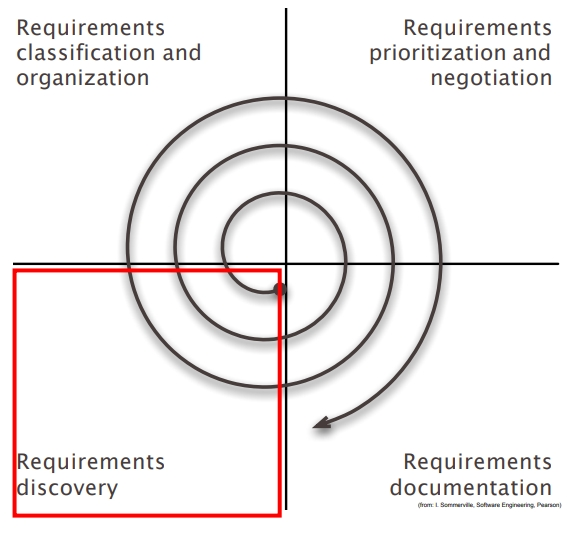
\includegraphics[width=0.5\textwidth]{Images/Requirements Elicitation and Analysis.jpeg}
\end{figure}
\begin{infoBox}[title=Viewpoint-orientierter Ansatz]
    Der \fatsf{Viewpoint-orientierte Ansatz} betrachtet die Anforderungen aus verschiedenen \fatsf{Blickwinkeln (Viewpoints)}, um sicherzustellen, dass alle relevanten Perspektiven abgedeckt sind. Dadurch wird das Risiko verringert, wichtige Anforderungen zu übersehen.
\end{infoBox}
\begin{defBox}[title=Systematic requirement descovery: Viewpoint-oriented Approach]
    \blue{Generic types of viewpoints}
    \begin{itemize}
        \item \red{Interactor} viewpoints: Persons (or systems) that will directly interact with the system such as end users, administrative \& servise personal \red{-direct stakeholders-}
        \item \red{Indirect} viewpoints: Stakeholders that influence the requirements, but who will not directly use the system, e.g. CFO (finances), data protection official \red{-indirect stakeholders-}
        \item \red{Domain} viewpoints: Domain characteristics \& constraints that influence the system requirements E.g., legal regulations on booking details and storage duration
    \end{itemize}
\end{defBox}
\begin{figure}
    \centering
    \begin{minipage}{0.3\textwidth}
        \centering
        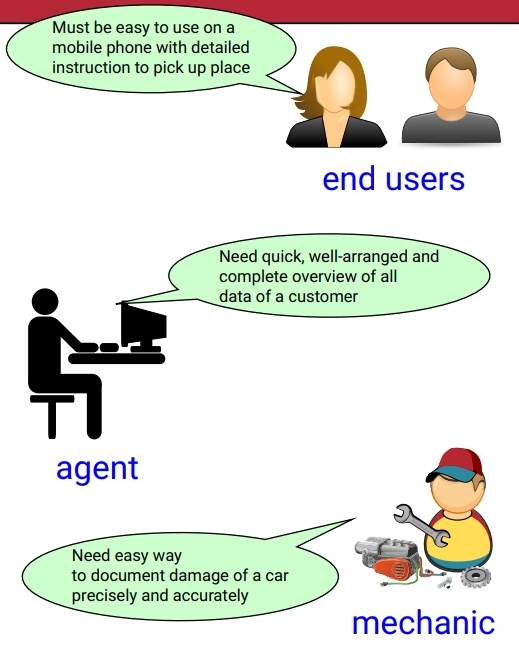
\includegraphics[width=\textwidth]{Images/Interactor viewpoints.jpeg}
        \caption{Interactor viewpoints}
    \end{minipage}\hfill
    \begin{minipage}{0.3\textwidth}
        \centering
        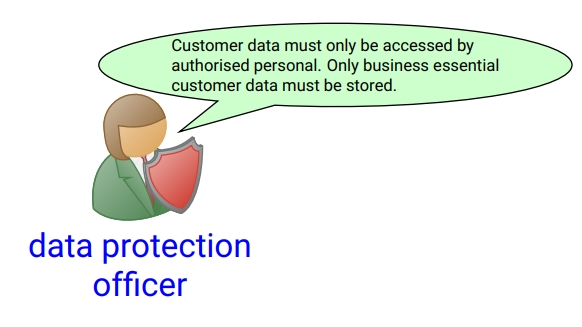
\includegraphics[width=\textwidth]{Images/Indirect viewpoints.jpeg}
        \caption{Indirect viewpoints}
    \end{minipage}\hfill
    \begin{minipage}{0.3\textwidth}
        \centering
        
\includegraphics[width=\textwidth]{Images/Domain viewpoints.jpeg}
        \caption{Domain viewpoints}
    \end{minipage}
\end{figure}
\begin{defBox}[title=Systematic requirement discovery: Viewpoint-oriented Approach]
    \begin{itemize}
        \item Develop more specific viewpoints during elicitation
        \begin{infoBox}
            \begin{itemize}
                \item Während der Anforderungsanalyse können neue, spezifischere Viewpoints identifiziert werden, die zunächst vielleicht nicht offensichtlich waren.
                \item Beispielsweise könnten im Laufe der Analyse weitere Stakeholdergruppen oder spezielle technische Anforderungen entdeckt werden, die vorher nicht berücksichtigt wurden.
                \item Das hilft, detaillierte Anforderungen zu erfassen, die sonst möglicherweise übersehen worden wären.
            \end{itemize}
        \end{infoBox}
        \item Use most important viewpoints to discover requirements
        \begin{infoBox}
            \begin{itemize}
                \item Nicht alle Viewpoints sind gleich wichtig, daher konzentriert man sich zuerst auf die wichtigsten Perspektiven, um die zentralen Anforderungen zu entdecken.
                \item Die wichtigsten Viewpoints sind in der Regel diejenigen, die den größten Einfluss auf das System haben oder am stärksten von den Ergebnissen betroffen sind, z.B. Endbenutzer oder gesetzliche Vorschriften.
                \item Das Priorisieren dieser Viewpoints hilft dabei, schnell die wesentlichen Anforderungen zu identifizieren, bevor man sich mit weniger wichtigen Details beschäftigt.
            \end{itemize}
        \end{infoBox}
    \end{itemize}
\end{defBox}

\begin{defBox}[title=Systematic requirement elicitation: Techniques: Interviews]
    \red{Closed interviews:} Predefined set of questions\\
    \red{Open interviews:} No predefined agenda\\
    \blue{Limitation:} Interviews should only be used as a \red{supplement}
    \begin{itemize}
        \item Bias of interviewee (e.g., afraid to loose job)
        \item Interviewee uses/assumes implicit domain knowledge
    \end{itemize}
\end{defBox}

\begin{defBox}[title=Systematic requirement elicitation: Further Techniques]
    \red{Scenario:} Sequence of interactions with system (next lecture)\\
    \red{Use Case} (next lecture)
\end{defBox}

\subsubsection*{Requirements Classification and Organization}
\begin{defBox}[title=Classification \& Organization]
    \begin{itemize}
        \item \blue{Given:} Unstructured collection of requirements
        \item \blue{Goal:} Requirements grouped \& organized into coherent clusters
    \end{itemize}
    One possible model for categorizing requirements: The \red{FURPS+} model
    \begin{itemize}
        \item Functional (Funktionalität)
        \begin{infoBox}
            \begin{itemize}
                \item Dies bezieht sich auf die \fatsf{Funktionen}, die das System bieten soll. Das sind spezifische Aufgaben, die das System ausführen muss, z.B. eine Suchfunktion in einer Anwendung.
            \end{itemize}
        \end{infoBox}
        \item Usability (Benutzbarkeit)
        \begin{infoBox}
            \begin{itemize}
                \item Diese Kategorie umfasst Anforderungen an die \fatsf{Benutzerfreundlichkeit} des Systems. Es geht um Aspekte wie Benutzeroberfläche, Barrierefreiheit und die Einfachheit der Nutzung.
            \end{itemize}
        \end{infoBox}
        \item Reliability (Zuverlässigkeit)
        \begin{infoBox}
            \begin{itemize}
                \item Hier geht es um die \fatsf{Zuverlässigkeit} des Systems, also darum, wie stabil und fehlerfrei es ist. Anforderungen in dieser Kategorie betreffen beispielsweise die Verfügbarkeit, Fehlertoleranz oder Ausfallsicherheit.
            \end{itemize}
        \end{infoBox}
        \item Performance (Leistung)
        \begin{infoBox}
            \begin{itemize}
                \item \fatsf{Leistungsanforderungen} beziehen sich auf die Effizienz des Systems, z. B. wie schnell es reagiert, wie viel Speicherplatz es benötigt oder wie viele Benutzer es gleichzeitig verarbeiten kann.
            \end{itemize}
        \end{infoBox}
        \item Supportability (Wartbarkeit)
        \begin{infoBox}
            \begin{itemize}
                \item Diese Kategorie umfasst Anforderungen, die die \fatsf{Wartbarkeit und Unterstützung} des Systems betreffen. Dazu gehören Aspekte wie die Möglichkeit, Fehler zu beheben, das System zu aktualisieren oder technische Unterstützung zu leisten.
            \end{itemize}
        \end{infoBox}
    \item \fatsf{\red{+}}
        \begin{itemize}
            \item Implementation (Implementierung)
            \begin{infoBox}
                Anforderungen an die technische Umsetzung, z. B. Programmiersprachen oder Standards, die einzuhalten sind.
            \end{infoBox}
            \item Interface (Schnittstellen)
            \begin{infoBox}
                Anforderungen an Schnittstellen zu anderen Systemen, z. B. Datenaustausch oder Integration.
            \end{infoBox}
            \item Operations (Betrieb)
            \begin{infoBox}
                Betriebsspezifische Anforderungen, z. B. Anforderungen an Systemadministration oder Überwachung.
            \end{infoBox}
            \item Packaging (Verpackung)
            \begin{infoBox}
                Anforderungen an die Bereitstellung des Systems, z. B. Installationspakete oder Dokumentation.
            \end{infoBox}
            \item Legal (Rechtliche Anforderungen)
            \begin{infoBox}
                Anforderungen aufgrund gesetzlicher Vorgaben, z. B. Datenschutz- oder Sicherheitsvorschriften.
            \end{infoBox}
        \end{itemize}
    \end{itemize}
\end{defBox}

\subsubsection*{Requirements Prioritization and Negotiation}
\begin{defBox}[title=Prioritization \& Negotiation]
    \begin{itemize}
        \item Requirements are prioritized
        \item Conflicts are found and resolved through negotiation
    \end{itemize}
\end{defBox}

\begin{infoBox}[title=Requirements Prioritization (Anforderungen priorisieren)]
    \begin{itemize}
        \item Wenn ein System oder eine Software entwickelt wird, gibt es oft viele Anforderungen, die erfüllt werden sollen. Allerdings sind Ressourcen wie \fatsf{Zeit}, \fatsf{Budget} und \fatsf{Personal} meistens begrenzt. Daher ist es notwendig, die Anforderungen nach ihrer \fatsf{Wichtigkeit und Dringlichkeit} zu priorisieren.
        \item Die Priorisierung hilft dabei, die Anforderungen in verschiedene Kategorien zu unterteilen, wie z.B.:
        \begin{itemize}
            \item \fatsf{Hoch:} Muss unbedingt erfüllt werden (kritische Anforderungen).
            \item \fatsf{Mittel:} Wichtige Anforderungen, die erfüllt werden sollten, aber nicht zwingend sofort.
            \item \fatsf{Niedrig:} Nice-to-have Anforderungen, die nur umgesetzt werden, wenn noch Ressourcen verfügbar sind.
        \end{itemize}
        \item Methoden zur Priorisierung:
        \begin{itemize}
            \item \fatsf{MoSCoW-Methode:} Unterteilt Anforderungen in \enquote{Must have}, \enquote{Should have}, \enquote{Could have} und \enquote{Won't have}.
            \item \fatsf{Kano-Modell:} Kategorisiert Anforderungen basierend auf ihrer Auswirkung auf die Kundenzufriedenheit.
            \item \fatsf{100-Punkte-Methode:} Stakeholder verteilen eine begrenzte Anzahl von Punkten auf die Anforderungen, um deren Priorität anzuzeigen.
        \end{itemize}
    \end{itemize}
\end{infoBox}
\begin{infoBox}[title=Requirements Negotiation (Anforderungen verhandeln)]
    \begin{itemize}
        \item \fatsf{Verhandlungen} sind notwendig, wenn es zu \fatsf{Konflikten} zwischen verschiedenen Anforderungen kommt, z.B. wenn unterschiedliche Stakeholder verschiedene Prioritäten haben oder wenn Anforderungen miteinander \fatsf{inkompatibel} sind.
        \item Ziel der Verhandlungen ist es, \fatsf{Kompromisse zu finden}, um Konflikte zu lösen und eine gemeinsame Übereinkunft zu erzielen.
        \item Es kann auch notwendig sein, Anforderungen anzupassen, zusammenzuführen oder zu streichen, um \fatsf{realistische Ziele} zu setzen und die vorhandenen Ressourcen optimal zu nutzen.
    \end{itemize}
\end{infoBox}
\begin{figure}[h]
    \centering
    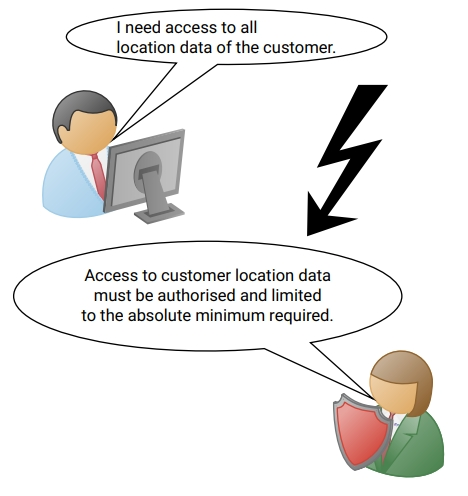
\includegraphics[width=0.35\textwidth]{Images/Prioritization und Negotiation.jpeg}
    \caption{Negotiation}
\end{figure}

\subsubsection*{Requirements Documentation}
\begin{defBox}[title=Documentation]
    The requirements are \red{documented} and used as \red{input} for the next iteration.\\
    The produced documents may be \red{formal} or \red{informal}.
\end{defBox}

\subsection{Requirements Documentation}
\subsubsection*{Software Requirements Specification Document (SRS)}

\begin{defBox}[title=Target group of SRS]
    Diverse set of stakeholders:
    \begin{itemize}
        \item Client, prospective users
        \item Managers (both on client and manufacturer side)
        \item System engineers, system test, and system maintenance engineers
        \item $\Rightarrow$ Anyone concerned with ordering, using, manufacturing, maintaining
    \end{itemize}
\end{defBox}
\begin{infoBox}
    Die Zielgruppe umfasst alle Personen, die in irgendeiner Weise mit dem \fatsf{Bestellen, Nutzen, Entwickeln oder Warten} der Software in Berührung kommen. Das SRS dient als gemeinsames Kommunikationsmittel, um sicherzustellen, dass alle Stakeholder die Anforderungen einheitlich verstehen.
\end{infoBox}
\begin{defBox}[title=Level of detail depends on ...]
    \begin{itemize}
        \item Type of system
        \item Development process
        \item Location of manufacture: external contractor or in-house
    \end{itemize}
\end{defBox}
\begin{infoBox}[title=Der Detaillierungsgrad des SRS hängt ab von ...]
    \begin{enumerate}
        \item \fatsf{Art des Systems}
        \begin{itemize}
            \item Ein komplexes System benötigt ein detailliertes SRS, während für kleinere, weniger komplexe Systeme ein einfacheres SRS ausreichen kann.
        \end{itemize}
        \item \fatsf{Entwicklungsprozess}
        \begin{itemize}
            \item In einem \fatsf{agilen Entwicklungsprozess} könnte das SRS eher allgemein sein und sich im Laufe der Zeit weiterentwickeln.
            \item In einem \fatsf{traditionellen Wasserfall-Modell} ist ein detailliertes und vollständiges SRS zu Beginn des Projekts erforderlich.
        \end{itemize}
        \item \fatsf{Ort der Fertigung: externer Auftragnehmer oder In-House\_Entwicklung}
        \begin{itemize}
            \item Wenn die Entwicklung durch einen \fatsf{externen Auftragnehmer} erfolgt, ist ein detailliertes SRS notwendig, um sicherzustellen, dass die Anforderungen klar und eindeutig sind.
            \item Bei einer \fatsf{In-House\_Entwicklung} kann das SRS flexibler sein, da die Entwickler näher am Projekt sind und schneller auf Änderungen reagieren können.
        \end{itemize}
    \end{enumerate}
\end{infoBox}

\subsection*{Structure of the Software Requirement Document}
\begin{defBox}[title=Requirements specification document (shortened from: ISO/IEC/IEEE 29148:2011)]
    \begin{enumerate}
        \item Introduction
        \begin{enumerate}
            \item Pupose of the requirements document (Zweck des Anforderungsdokuments)
            \begin{infoBox}
                Beschreibt, warum das Dokument erstellt wurde und welche Ziele es hat. Es legt fest, für wen das Dokument gedacht ist und welchen Nutzen es bietet.
            \end{infoBox}
            \item \blue{Scope of the product} (Umfang des Produkts)
            \begin{infoBox}
                Definiert, was das System leisten soll, also den \fatsf{Anwendungsbereich} des Produkts. Hier wird auch beschrieben, \fatsf{was nicht im Umfang enthalten} ist, um Messverständnisse zu vermeiden.
            \end{infoBox}
            \item Definitions, acronyms and abbreviations (Definitionen, Akronyme und Abkürzungen)
            \item References (Referenzen)
            \begin{infoBox}
                Eine Liste von \fatsf{Dokumenten, Standards} oder \fatsf{anderen Quellen}, auf die im Anforderungsdokument Bezug genommen wird.
            \end{infoBox}
            \item Overview (Überblick)
            \begin{infoBox}
                Eine \fatsf{kurze Zusammenfassung} des Dokuments, die beschreibt, wie es organisiert ist und welche Inhalte in den folgenden Abschnitten zu erwarten sind.
            \end{infoBox}
        \end{enumerate}
        \item General description
        \begin{enumerate}
            \item \blue{Product perspective}
            \begin{infoBox}
                Beschreibt, wie sich das System in \fatsf{andere Systeme} oder \fatsf{bestehende Produkte} einfügt, einschließlich seiner Schnittstellen und Abhängigkeiten.
            \end{infoBox}
            \item Product functions
            \begin{infoBox}
                Eine allgemeine Beschreibung der \fatsf{Hauptfunktionen}, die das System bereitstellen soll.
            \end{infoBox}
            \item \blue{User characteristics} (Benutzermerkmale)
            \begin{infoBox}
                Beschreibt die \fatsf{Zielgruppe} des Produkts, z.B. die \fatsf{Erfahrung} oder \fatsf{technischen Fähigkeiten} der Benutzer.
            \end{infoBox}
            \item Limitations (Einschränkungen)
            \begin{infoBox}
                Nennen von \fatsf{Einschränkungen} oder \fatsf{Bedingungen}, die bei der Entwicklung betrachtet werden müssen, z.B. rechtliche Anforderungen oder technische Grenzen.
            \end{infoBox}
            \item Assumptions and dependencies (Annahmen und Abhängikeiten)
            \begin{infoBox}
                \fatsf{Annahmen}, die während der Anforderungsanalyse gemacht wurden, und \fatsf{Abhängigkeiten}, die das System betreffen.
            \end{infoBox}
        \end{enumerate}
    \end{enumerate}
\end{defBox}
 \begin{defBox}
    \begin{enumerate}[start=3]
        \item Specific requirements (Spezifische Anforderungen)
        \begin{infoBox}
            Dieser Abschnitt enthält die detaillierten \fatsf{funktionalen} und \fatsf{nicht-funktionalen} Anforderungen. Es handelt sich um eine \fatsf{ausführliche Beschreibung} dessen, was das System leisten muss, und wie es sich unter bestimmten Bedingungen verhalten soll.
        \end{infoBox}
        \item Appendices, Index, etc. (Anhänge, Index usw.)
        \begin{infoBox}
            \begin{itemize}
                \item \fatsf{Anhänge} können zusätzliche Informationen enthalten, die für das Verständnis des Dokuments nützlich sind, z.B. \fatsf{Flussdiagramme, technische Spezifikationen} oder \fatsf{Beispiele.}
                \item Ein \fatsf{Index} hilft, bestimmte Abschnitte oder Begriffe im Dokument schnell zu finden.
            \end{itemize}
        \end{infoBox}
    \end{enumerate}
\end{defBox}
\begin{itemize}
    \item \red{1.b Scope of product:} Can also contain what is \red{not} in scope
    \begin{infoBox}
        Kann auch beschreiben, \fatsf{was nicht im Umfang enthalten} ist, um die Grenzen des Projekts klar fetzulegen.
    \end{infoBox}
    \item \red{1.c Glossary:} Explains ambiguous or technical terms, expand abbreviations
\end{itemize}

\subsection{Requirements Engineering Process}
\subsubsection*{Requirement Validation}
\begin{defBox}[title=Requirement Validation Checkpoints]
    \begin{itemize}
        \item \red{Validity} (Gültigkeit)
        \begin{itemize}
            \item Do the requirements \red{capture} the needed features?
            \item Is \red{additional} or other functionality needed?
        \end{itemize}
        \item \red{Consistency} (Konsistenz)
        \begin{itemize}
            \item Check that the requirements are \red{not conflicting}
        \end{itemize}
        \item \red{Completeness} (Vollständigkeit)
        \begin{itemize}
            \item Do the requirements define \red{all} functions and constraints as intended by the system user?
        \end{itemize}
        \item \red{Realism} (Realisierbarkeit)
        \begin{itemize}
            \item Can the requirements reasonably be implemented? (Refinement of feasibility study)
        \end{itemize}
        \item \red{Traceability} (Rückverfolgbarkeit)
        \begin{itemize}
            \item Is each requirement traceable to its source (where does each requirement derive from)?
            \begin{infoBox}
                \begin{itemize}
                    \item Jede Anforderung sollte auf ihren \fatsf{Ursprung} zurückgeführt werden können, d.h. es sollte klar sein, woher die Anforderung stammt (z.B. ein bestimmter Stakeholder, eine gesetzliche Vorschrift).
                    \item Die Rückverfolgbarkeit hilf dabei, \fatsf{Änderungen} an den Anforderungen nachzuvollziehen und sicherzustellen, dass alle Anforderungen korrekt abgedeckt sind.
                \end{itemize}
            \end{infoBox}
        \end{itemize}
    \end{itemize}
\end{defBox}
\clearpage
\section{Use Cases Analysis}
\subsection{What? vs How?}
\begin{defBox}[title=Requirements... \enquote{Anforderungen}]
    \begin{itemize}
        \item ...focus on the desired \red{functionality} and \red{operational constraints}
        \item ...are often stated \red{declaratively}
    \end{itemize}
    Perspective of the \red{Client}
\end{defBox}
\begin{defBox}[title=Use Cases... \enquote{Anwendungsfälle}]
    \begin{itemize}
        \item ...identify anticipated \red{interaction} sequences: \red{scenarios}
        \item ...are stated \red{operationally}
    \end{itemize}
    Perspective of the \red{User}
\end{defBox}
\begin{infoBox}
    \begin{itemize}
        \item \fatsf{Anforderungen} beschreiben abstrakt, was das System leisten soll, aus der Perspektive des Kunden, und geben keine Details zur Umsetzung an.
        \item \fatsf{Anwendungsfälle} beschreiben detailliert, wie Benutzer mit dem System interagieren, aus der Perspektive des Benutzers, und sind auf konkrete Abläufe fokussiert.
    \end{itemize}
\end{infoBox}
\begin{figure}[h]
    \centering
    \includegraphics[width=1\textwidth]{Images/What? vs How?.jpeg}
\end{figure}
\subsection{Use Cases: Effort on the Client Side}
\begin{defBox}
    Impossible to write good/complete uses cases without \red{user involvement}
\end{defBox}
\begin{defBox}[title=A Common Misconception]
    Software cost \~ development cost, but in fact:
    \begin{itemize}
        \item Need to allocate at least 30-50\% of development cost \red{at client side} for requirements/use case analysis + validation
        \item Need to allocate ongoing budget for \red{maintenance}
    \end{itemize}
\end{defBox}
\subsection{The CaSh Case Study}
\begin{defBox}[title=Main Roles \& Functionalities (from requirements identification)]
    \blue{General}
    \begin{itemize}
        \item Authentication
    \end{itemize}
    \blue{Administrator}
    \begin{itemize}
        \item Add/change new cars, rental locations
        \item Billing
    \end{itemize}
    \blue{User}
    \begin{itemize}
        \item Check availability
        \item Request booking
        \item \red{Change booking}
    \end{itemize}
    \blue{Service Person}
    \begin{itemize}
        \item Take out vehicle for service
    \end{itemize}
\end{defBox}

\subsection{Text Stories}
\begin{defBox}[title=Change Existing Booking]
    An authenticated customer wants to change an existing booking.\\
    The customer selects the booking to change. The system displays the booking details, including adjacent reservations. The customer is offered to change the reserved duration, or else to cancel the reservation. The customer is offered to change the reserved duration, or else to cancel the reservation.\\
    When a new duration is entered, the system checks availability and records the change. In case of no availability, nothing happens and an information message is displayed.\\
    if the customer chooses to cancel the booking, then it is removed.\\
    Before any change happens, incurred cost is displayed, and a confirmation action is requested. After each change, a confirmation message is sent to the customer's preferred contact.
\end{defBox}
\subsection{Use Cases}
\begin{defBox}
    \begin{itemize}
        \item Use cases are \red{text stories} used to discover and record requirements
        \item Use cases \red{complement} requirements analysis
        \item Use cases provide \red{operational} requirements as a basis for system design
    \end{itemize}
\end{defBox}
\red{Attention:}
\begin{itemize}
    \item Use cases $\neq$ User stories
    \item Use cases are \red{not a replacement} of requirements analysis (do not capture non-functional requirements)
\end{itemize}

\begin{infoBox}
    \begin{itemize}
        \item \fatsf{Use Cases} sind detaillierte Geschichten, die helfen, die \fatsf{Anforderungen zu verstehen} und zu dokumentieren, um später das \fatsf{Systemdesign} darauf aufzubauen.
        \item Sie ergänzen die \fatsf{Anforderungsanalyse} und liefern \fatsf{operative Details}, die als Grundlage für die Entwicklung dienen.
        \item \fatsf{User Stories} sind kürzer und fokussieren sich auf \fatsf{Zielsetzungen}, während \fatsf{Use Cases} konkrete \fatsf{Interaktionsabläufe} detailliert beschreiben.
    \end{itemize}
\end{infoBox}

\subsection{Constituents of Use Cases: Some Definitions}
\red{Actor} Someone or something with \red{behavior}: a person, computer system, an organization, etc.
\begin{itemize}
    \item \red{Primary actor} The actor who requests a service from the system (\blue{initiates} the use case)
\end{itemize}
\red{Scenario} (also known as a \blue{use case instance}) A \red{specific sequence of actions} and interactions between actor and the system
\begin{itemize}
    \item \blue{One} particular story using a system
\end{itemize}
\red{Use case} A \red{collection of} related success and failure \red{scenarios} that describe an actor's usage of a system to achieve a goal

\begin{infoBox}
    \begin{enumerate}
        \item \fatsf{Actor (Akteur)}
        \begin{itemize}
            \item Ein \fatsf{Akteur} ist \fatsf{jemand oder etwas}, das ein Verhalten zeigt und mit dem System interagiert. Das kann eine \fatsf{Person}, ein \fatsf{Computer-System}, eine \fatsf{Organisation} oder sogar ein \fatsf{anderes System sein}.
            \item Der Akteur spielt eine wichtige Rolle in einem Use Case, da er mit dem System interagiert, um ein Ziel zu erreichen. Akteure sind die \enquote{Benutzer} oder \enquote{Stakeholder}, die vom System einen bestimmten Service oder eine Funktionalität anfordern.
        \end{itemize}
        \item Primary Actor (Primäre Akteur)
        \begin{itemize}
            \item Der \fatsf{primäre Akteur} ist der Akteur, der \fatsf{eine Dienstleisung} oder Funktion vom System anfordert und somit den Use Case \fatsf{initiiert}. In den meisten Fällen handelt es sich um den Benutzer, der mit dem System interagiert, aber es kann auch ein anderes System sein, das den Use Case auslöst.
            \item Beispiel: In einem Online-Shop könnte der \fatsf{primäre Akteur} ein \fatsf{Kunde} sein, der ein Produkt kauft.
        \end{itemize}
        \item Scenario (Szenario)
        \begin{itemize}
            \item Ein \fatsf{Szenario (auch als \fatsf{Use Case Instance} bezeichnet) ist eine \fatsf{spezifische Abfolge von Aktionen und Interaktionen} zwischen einem Akteur und dem System. Es beschreibt den Ablauf, wie ein Akteur in einem bestimmten Fall mit dem System interagiert.}
            \item Ein Szenario ist im Grunde genommen eine konkrete \fatsf{Geschichte}, wie der Akteur das System in einer bestimmten Situation nutzt. Es beschreibt, welche Schritte der Akteur ausführt und wie das System darauf reagiert.
            \item Beispiel: Ein Szenario könnte die Schritte beschreiben, die ein Kunde durchführt, um sich in einen Online-Shop einzuloggen und ein Produkt zu kaufen.
        \end{itemize}
        \item \fatsf{Use Case (Anwendungsfall)}
        \begin{itemize}
            \item Ein \fatsf{Use Case} ist eine Sammlung von \fatsf{zusammenhängenden Szenarien}, die den gesamten Ablauf und die verschiedenen Möglichkeiten beschreiben, wie ein Akteur mit einem System interagiert, um ein bestimmtes Ziel zu erreichen.
            \item Der Use Case umfasst sowohl \fatsf{Erfolgsszenarien} (also die Szenarien, in denen das Ziel des Akteurs erfolgreich erreicht wird, möglicherweise aufgrund von Fehlern oder Problemen im System).
            \item Ein Use Case stellt somit eine vollständige \fatsf{Beschreibung des Verhaltens des Systems} dar, das den Akteur bei der Erreichung seines Ziels unterstützt.
            \item Beispiel: Ein Use Case für einen Online-Shop könnte sowohl das Szenario des erfolgreichen Kaufabschlusses als auch Szenarien wie den Abbruch des Kaufs aufgrund einer ungültigen Zahlungsmethode umfassen.
        \end{itemize}
    \end{enumerate}
\end{infoBox}

\subsection{Different Kinds of Use Cases (Other distinctions exist)}
\red{White box vs. Black box} - with whom does interaction take place?
\begin{itemize}
    \item \red{White box} (\enquote{Transparent}) use cases provide a detailed view of \blue{interaction of internals} when satisfying a user goal
    \item \red{Black box} use cases encapsulate the system and describe \blue{only interactions with external actors}
\end{itemize}
\red{Corporate vs. System}
\begin{itemize}
    \item \red{Corporate} (\enquote{geschäftlich}) use cases describe a \blue{business process} (often without mentioning the system under design)
    \item \red{System} use cases are performed and described with respect to the \blue{system under design}
\end{itemize}
\begin{defBox}[title=Defaults]
    \begin{itemize}
        \item Corporate use cases are usually \red{white box} use cases 
        \item System use cases are in their vast majority \red{black box} use cases
    \end{itemize}
\end{defBox}

\subsection{Use Case Formats}
\begin{itemize}
    \item \red{Brief} (\enquote{kurz}) Terse one-paragraph summary, usually main success scenario
    \item \red{\enquote{informell}} Informal paragraph format; multiple paragraphs that cover various scenarios \blue{(as seen above)}
    \item \red{Fully Dressed} (\enquote{ausgearbeitet}) All steps and variations written in detail; there are supporting sections, such as preconditions and success guarantees
\end{itemize}
\begin{infoBox}
    \begin{itemize}
        \item \fatsf{Whitebox vs. Blackbox} unterscheidet, ob interne Abläufe im system sichtbar sind (Whitebox) oder ob nur die externen Interaktionen dargestellt werden (Blackbox).
        \item \fatsf{Corporate vs. System} unterscheidet, ob der Fokus auf einem gesamten Geschäftsprozess liegt (Coporate) oder auf einem System, das entwickelt wird (System).
    \end{itemize}
\end{infoBox}
\begin{defBox}[title=Precision vs. Accuracy (\enquote{Detaillierungsgrad} bzw. \enquote{Zutreffendheit})]
    \red{Precision:} Level of detail provided by the use case description: granularity\\
    \red{Accuracy:} Correctness-is the description of the use case correct for the amount of detail given?
\end{defBox}
\subsection{Template for Fully Dressed Use Case}
\begin{table}[H]
    \centering
    \rowcolors{2}{\thepagecolor}{fgcolor!10!\thepagecolor}
    \renewcommand{\arraystretch}{1.2}
    \begin{tabular}{lll}
        \toprule
        Use Case Section & Purpose/Guidelines \\
        \midrule
        Use Case Name & Start with a verb \enquote{Accomplish this task} \\
        Scope(\enquote{Umfang}) & Corporate, system (better: name), subsystem \\
        Level(\enquote{Ebene}) & Unser goal, summary goal subfunction \\
        Preconditions & What must be true at start \& worth telling the reader\\
        Minimal Guarantee & Fewest promises system makes to stakeholder\\
        Success Guarantee & What must be true on successful completion \& and is worth telling the reader\\
        Main Success Scenario & Representative scenario of successful use case execution\\
        Extensions & Alternative scenarios of success or failure\\
        Terchnologie and Data Variation List & Varying I/O methods and data formats\\
        Frequency of Occurrence & Influences inverstigation, testing and timing of implementation\\
        Miscellaneous & For example, open issues\\
        \bottomrule
    \end{tabular}
\end{table}

\begin{infoBox}[title=Use Case Name]
    \begin{itemize}
        \item Der Name des Use Cases sollte \fatsf{mit einem Verb beginnen} und das Ziel klar formulieren, z.B. \enquote{Abschließen einer Bestellung} oder \enquote{Erstellen eines Benutzerkontos}. Damit wird sofort ersichtlich, \fatsf{welche Aufgabe} der Use Case abdeckt.
    \end{itemize}
\end{infoBox}
\begin{infoBox}[title=Scope(Umfang)]
    \begin{itemize}
        \item Der \fatsf{Umfang} definiert, auf welcher Ebene der Use Case wirkt:
        \begin{itemize}
            \item \fatsf{Corporate:} Unternehmensweit, also ein gesamter Geschäftsprozess.
            \item \fatsf{System:} Ein spezifisches System, das in Entwicklung ist.
            \item \fatsf{Subsystem:} Ein bestimmter Teil eines Systems.
        \end{itemize}
        \item Die Angabe des Umfangs hilft dabei, den Rahmen und die Grenzen des Use Cases klarzustellen.
    \end{itemize}
\end{infoBox}
\begin{infoBox}[title=Level(Ebene)]
    \begin{itemize}
        \item Die Ebene beschreibt den \fatsf{Detaillierungsgrad} des Use Cases:
        \begin{itemize}
            \item \fatsf{User Goal:} Das zentrale Ziel des Benutzers, das den größten Wert liefert.
            \item \fatsf{Summary Goal:} Ein zusammenfassendes Ziel, das \fatsf{mehrere User Goals} abdeckt und den Kontext des Systems beschreibt.
            \item \fatsf{Subfunction:} Eine Funktion, die Teil eines User Goals ist und \fatsf{weiderverwendbar} sein kann.
        \end{itemize}
    \end{itemize}
\end{infoBox}
\begin{infoBox}[title=Preconditions(Vorbedingungen)]
    \begin{itemize}
        \item Die Vorbedingungen beschreiben, \fatsf{was wahr sein muss}, bevor der Use Case beginnen kann.
        \item Sie werden vom System \fatsf{sichergestellt} und \fatsf{nicht während der Ausführung} erneut überprüft. Ein Beispiel wäre, dass der Benutzer bereits angemeldet ist.
    \end{itemize}
\end{infoBox}
\begin{infoBox}[title=Minimal Guarantee (Minimale Garantie)]
    \begin{itemize}
        \item Die Minimalgarantie ist das \fatsf{Mindeste, was das System den Stakeholdern verspricht}, selbst wenn das Hauptziel des Use Cases nicht erreicht wird.
        \item Diese Garantie beschreibt, wie das System in jedem Fall \fatsf{einen Basiswert liefert.} Beispiel: Das System hat alle bisherigen Schritte protokolliert, auch wenn die Bestellung nicht abgeschlossen wurde.
    \end{itemize}
\end{infoBox}
\begin{infoBox}[title=Success Guarantee (Erfolgsgarantie)]
    \begin{itemize}
        \item Die Erfolgsgarantie gibt an, welche \fatsf{Interessen der Stakeholder} nach erfolgreichem Abschluss des Use Cases \fatsf{erfüllt} sein müssen.
        \item Sie ergänzt die Minimalgarantie und wird \fatsf{am Ende des erfolgreichen Hauptszenarios} oder eines alternativen Erfolgspfads definiert. Beispiel: Nach Abschluss ist die Bestellung gespeichert und bestätigt.
    \end{itemize}
\end{infoBox}
\begin{infoBox}[title=Main Success Scenario (Haupt-Erfolgsszenario)]
    \begin{itemize}
        \item Das Haupt-Erfolgsszenario beschreibt die \fatsf{repräsentative Schritt-für-Schritt-Sequenz} eines \fatsf{erfolgreichen Use Case Ablaufs.}
        \item Die Schritte sind \fatsf{nummeriert} und beinhalten die wichtigsten Aktionen, um das Ziel zu erreichen. Der erste Schritt beschreibt oft den \fatsf{Trigger} des Use Cases, also die Aktion, die ihn startet.
    \end{itemize}
\end{infoBox}
\begin{infoBox}[title=Extensions (Erweiterungen)]
    \begin{itemize}
        \item Erweiterungen sind \fatsf{Abweichungen} vom Hauptszenario und beschreiben alternative Pfade oder Fehlerbehandlungen.
        \item Sie beziehen sich \fatsf{eindeutig auf Schritte} im Haupt-Erfolgsszenario, die variieren könnten, und verwenden ein strukturiertes Format:
        \begin{itemize}
            \item Beispiel: Wenn Schritt 2 verändert wird, könnten die Varianten 2.a, 2.b usw. heißen.
            \item Jeder Schritt innerhalb einer Variante ist nummeriert, z.B. 2.a.1 für den ersten Schritt in Variante 2.a.
        \end{itemize}
    \end{itemize}
\end{infoBox}
\begin{defBox}[title=Two fundamental types of scope]
    \begin{itemize}
        \item \red{Design Scope:} \blue{Specified in this row} Defines boundaries of system of the use case (whole corporation, (sub-)system name)
        \item \red{Function Scope} 
        \begin{itemize}
            \item Limits functionality to be realized by system under design 
            \item Managed by a list of functions in and out of scope
        \end{itemize}
    \end{itemize}
\end{defBox}
\begin{defBox}[title=Kinds of goals]
    \begin{itemize}
        \item \red{User goal} \blue{Most important} elementary goal of user that produces value
        \item \red{Summary Goal} Multiple user goals: describes \red{context} of system under design \blue{or} life-cycle \red{sequence} of related goals \blue{or} \red{table of content} for lower-level use cases
        \item \red{Subfunction}
        \begin{itemize}
            \item Use case being \red{part of} a user goal
            \item singled out on a by-need basis, \red{reusable} in multiple goals
        \end{itemize}
    \end{itemize}
\end{defBox}
\begin{defBox}[title=Stakeholder \enquote{Teilhaber}]
    Subject or object with interest in the behavior of the system under design: Company stakeholder, customer, vendor, regulatory agency, ...
\end{defBox}

\subsection{Use Case Extension for CaSh Change Booking}
\begin{defBox}[title=Change Booking]
    When a new duration is supplied, the system checks availability and records the change. In case of no availability, nothing happens and an information message is displayed.\\
    \red{If the given duration isidentical to the reserved period, then nothing happens.}
    Before any change happens, incurred cost in displayed, and a confirmation action is requested.\\
    \red{If the session times out before confirmation is given, nothing happens.}
\end{defBox}

\subsection{Excerpt of Fully Dressed Use Case}
\begin{table}[H]
    \centering
    \rowcolors{2}{\thepagecolor}{fgcolor!10!\thepagecolor}
    \renewcommand{\arraystretch}{1.2}
    \begin{tabular}{lll}
        \toprule
        Use Case Section & Purpose/Guidelines \\
        \midrule
        Name & List Available Cars\\
        Scope & CaSh Booking Module\\
        Level & User goal\\
        Primary Actor & CaSh Customer\\
        Stakeholders and Interests & \red{Customer:} wants to find available cars for a given duration and location.\\
         & \red{CaSh Company:} wants to make accurate offer\\
        Precondition & Customer is authenticated\\
        Minimal guarantee & No side effects\\
        Success guarantee & All available cars of requested class, specified duration, and location are displayed to customer\\
        Main Success Scenario & 1. Customer wants to know whether there is a suitable car to book\\
         & 2. Customer enters address or uses location service;\\
         & enters maximal location distance or use default\\
         & 3. Customer enters desired reservation period\\
         & 4. System validates time period\\
         & 5. Customer completes search details by entering desired class of car\\
         & 6. System determines matching options\\
         & 7. System displays all available cars matching selction criteria\\
          Extensions & 3.a End date is equal to or before start date\\
         & 3.a.1 Ask customer to specify non-empty period\\
         & 5.a Session times out before search details completed\\
         & 5.a.1 Customer is logged out\\
         & 7.a Search criteria give no result\\
         & 7.a.1 System includes cars one class lower and higher\\
         & 7.a.2 System includes cars with partial overlap of requested duration\\
         & 7.a.3 System suggests to customer to increase location distance\\
        \bottomrule
    \end{tabular}
\end{table}

\subsection{Guidelines for Developing Use Cases}
\begin{defBox}[title=In General: Proceed Incrementally]
    \begin{enumerate}
        \item Identify all currently relevant use cases accurately at a \red{very high level}
        \item Add precision \red{gradually}, work out the details
    \end{enumerate}
\end{defBox}

\begin{defBox}[title=Recommended Workflow]
    \begin{enumerate}
        \item List supported \red{acoters} \& their \red{goals}\\
        Review list for accuracy and completeness\\
        \blue{Outcome:} first level of precision of functional requirements
        \item Write \red{stakeholders}, \red{trigger}, and \red{main success scenario} for each use case\\
        \red{Validate} that the system delivers to important stakeholders\\
        \blue{Outcome:} second level of precision for functional requirements
        \item Identify and list all \red{failure conditions}
        \item Write \red{failure handling}\\
        \blue{Do not interleave} this step with the previous one:\\
        Danger of not completing list of all failures
    \end{enumerate}
\end{defBox}

\subsection{Further Recommendations for Writing Use Cases}
\begin{itemize}
    \item During early requirements work: \red{Keep the user interface out} (Focus on \red{intent})
    \item Write \red{terse} use cases
    \item Write \red{black box} use cases: Describe \red{what} the system must do and \red{not how}\\
    For instance:\\
    \enquote{The system records the booking.} (korrekt)
    \enquote{The system writes the booking to a database.} (falsch)
    \item Take an \red{actor} or actor-goal perspective
    \item Focus on the \red{users} or \red{acotors} of a system:
    \begin{itemize}
        \item Ask about their \red{goals} and typical situations
        \item Focus on understanding what the actor considers a \red{valuable result}
    \end{itemize}
\end{itemize}
\begin{defBox}
    Identifying and writing good use cases may take weeks
\end{defBox}

\subsection{Which of these phrases is a valid use case?}
\subsubsection*{Examples}
\begin{itemize}
    \item Negotiate a supplier contact
    \item Handle returned sale
    \item Log in 
    \item Move piece on game board
\end{itemize}

\subsubsection*{Checklist}
\begin{itemize}
    \item Is it a well-defined \red{task} ...
    \begin{itemize}
        \item performed by \red{one stakeholder} in one place at one time,
        \item to model a \red{business event}, 
        \item which \red{adds measurable business value} and
        \item leaves the data in a \red{consistent state}?
    \end{itemize}
    This is called \red{Elementary Business Process (EBP)}
    \item Is it not merely a single step (\blue{size test})?
\end{itemize}

\begin{defBox}[title=Which of these phrases is a valid use case?]
    \begin{itemize}
        \item Negotiate a supplier contract: (no) too complex-no \red{elementary} business case
        \item Handle retruned sale: (yes)
        \item Log in: (no) Depends on context, usually does not add value to business case
        \item Move piece on game board: (no) Single step, fails size test
    \end{itemize}
\end{defBox}

\section{UML Use Case Diagrams}
\subsection{The Unified Modeling Language (UML)}
\begin{defBox}[title=Some Facts]
    \begin{itemize}
        \item The Unified Modeling Language (UML) is a \red{visual}, yet precise, \red{design notation} for software development
        \item Originated as merger of the three OO modelling approaches: \blue{Booch, OMT, OOSE}- as well as best practices
        \item Maintained and developed by the Object Modeling Group (OMG)
        \item Main \red{goal}: support object modelling \red{tool interoperability} by agreeing on syntax and semantics of underlying modelling language
        \item Consists of collection of \red{diagrammatic modelling notations}, including:
        \begin{itemize}
            \item \red{Use case} diagram
            \item \red{Class}, object, package diagram
            \item Sequence, collaboration, activity diagram
            \item \red{State} diagram, ... + ca. 10 more
        \end{itemize}
    \end{itemize}
\end{defBox}
\begin{infoBox}[title=Sammlung von diagrammatischen Modellierungsnotationen:]
    \begin{itemize}
        \item UML besteht aus \fatsf{verschiedenen Diagrammtypen}, die unterschiedliche Aspekte eines Systems abbilden. Die gängigsten UML-Diagramme sind:
        \begin{itemize}
            \item \fatsf{Use Case Diagram:} Zeigt die Interaktionen zwischen dem System und seinen Akteuren.
            \item \fatsf{Class Diagram:} Stellt die Klassenstruktur eines Systems dar und zeigt Beziehungen zwischen Klassen.
            \item \fatsf{Object Diagram:} Zeigtdie Instanzen von Klassen zu einem bestimmten Zeitpunkt und deren Beziehungen.
            \item \fatsf{Package Diagram:} Organisiert Klassen und andere Elemente in Gruppen.
            \item \fatsf{Sequence Diagram:} Stellt die zeitliche Reihenfolge der Interaktionen zwischen Objekten dar.
            \item \fatsf{Collaboration Diagram:} Zeigt, wie Objekte miteinander kommunizieren, um eine Aufgabe zu erfüllen.
            \item \fatsf{Activity Diagram:} Stellt Workflows und Aktivitäten in einem Prozess dar.
            \item \fatsf{State Diagram:} Beschreibt die Zustände eines Objekts und die Übergänge zwischen diesen Zuständen.
        \end{itemize}
        \item Insgesamt umfasst UML rund \fatsf{14 verschiedene Diagrammtypen}, die verschiedene Aspekte eines Systems abdecken.
    \end{itemize}
\end{infoBox}
\begin{infoBox}
    UML ist eine \fatsf{standardisierte Modellierungssprache}, die aus mehreren Diagrammtypen besteht und speziell entwickelt wurde, um \fatsf{objektorientierte System visuell zu modellieren.} Sie erleichtert das Design komplexer Systeme, indem sie eine klare, visuelle und universelle Noatation für Entwicklerteams weltweit bietet.
\end{infoBox}

\subsection{UML Use Case Diagram}
\begin{figure}[h]
    \centering
    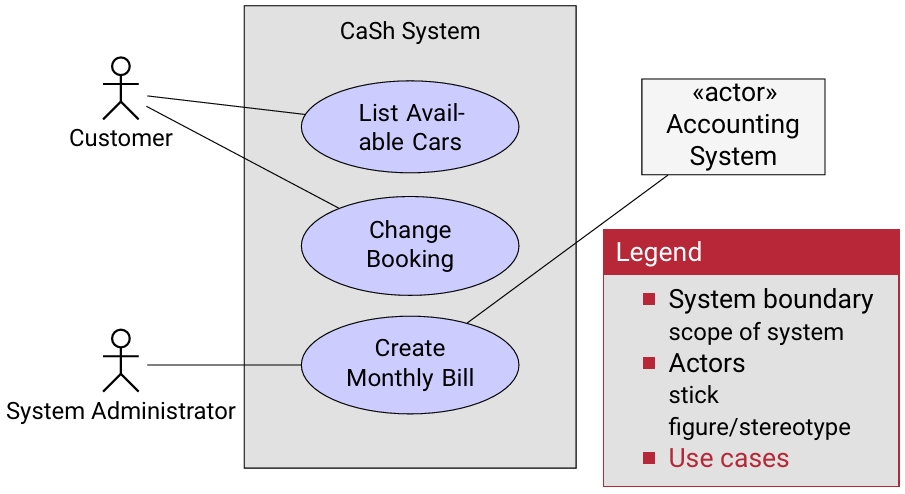
\includegraphics[width=1\textwidth]{Images/UML Use Case Diagram.jpeg}
\end{figure}

\subsection{Remarks on UML Use Case Diagrams}
\begin{itemize}
    \item UML use case diagram notation is intentionally \red{minimalist}
    \item UML use case diagrams are \red{organizational method} to improve
    \begin{itemize}
        \item communication and comprehension of use cases
        \item to reduce text duplication
    \end{itemize}
\end{itemize}
\begin{defBox}
    Organizing use cases into relationships has no impact on the behavior or requirements of a system
\end{defBox}
\begin{itemize}
    \item Use case diagrams provide a \red{black-box view} on a software system
    \item Use case diagrams are helpful only during \red{early} phase of use case analysis
\end{itemize}
\begin{itemize}
    \item \blue{Unsuitable to represent fully dressed use cases}
\end{itemize}

\clearpage
\subsection{The UML Use Case <<include>> Relation}
\begin{figure}[h]
    \centering
    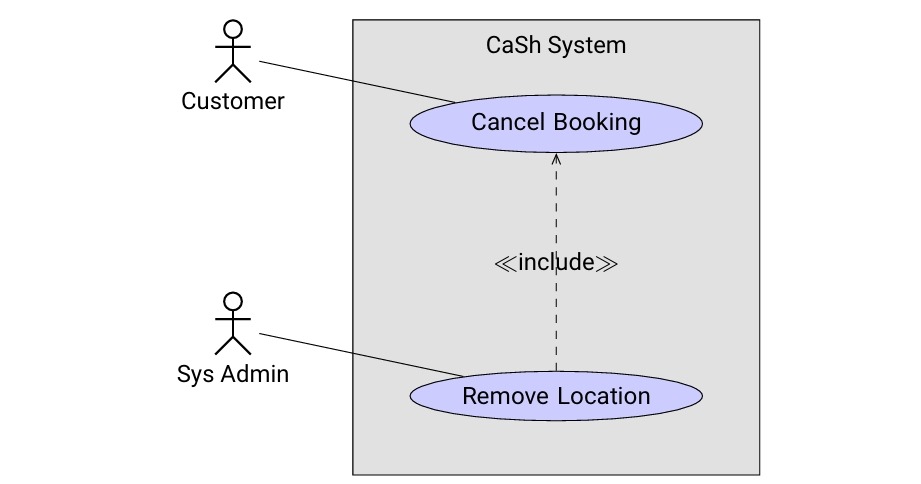
\includegraphics[width=1\textwidth]{Images/The UML Use Case include Relation.jpeg}
\end{figure}
\begin{defBox}[title=Include Relation]
    Factor out \red{common behaviour} across several use cases into its own sub-function use case and indicate inclusion\\
    \red{Facilitates decomposition of large use cases and enables reuse}
\end{defBox}
\begin{defBox}
    Included use cases are always executed
\end{defBox}
\begin{infoBox}
    Die \fatsf{<<include>>-Beziehung} in UML-Anwendungsfalldigrammen dient dazu, \fatsf{gemiensames Verhalten aus mehreren Anwendungsfällen herauszulösen} und in einem eigenen \fatsf{Unteranwendungsfall} (Sub-Use-Case) zu definieren. Diese Vorgehensweise ermöglicht eine klare Struktur und Wiederverwendbarkeit.
\end{infoBox}

\clearpage
\subsection{The UML Use Case <<extend>> Relation}
\begin{figure}[h]
    \centering
    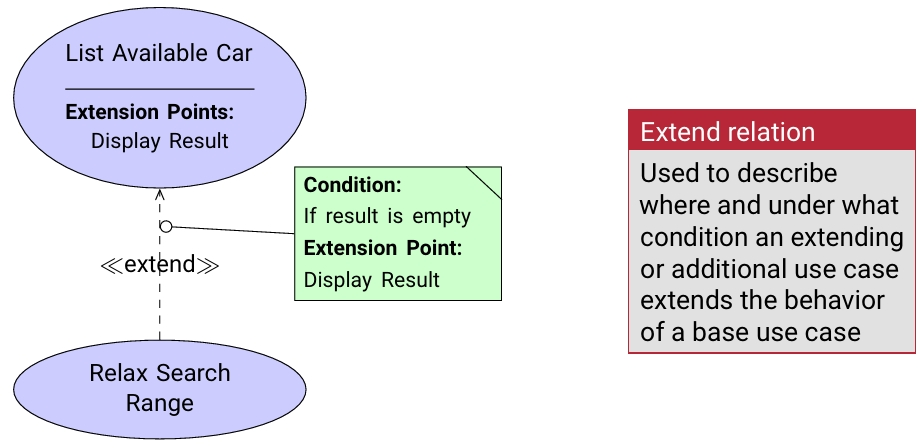
\includegraphics[width=1\textwidth]{Images/extend Relation.jpeg}
\end{figure}
\begin{infoBox}
    Die <<extend>>-Beziehung wird genutzt, um \fatsf{zusätzlich Funktionalität} zu beschreiben, die nur unter bestimmten Bedingungen in einem Anwendungsfall ausgeführt wird. Dies ist hilfreich, wenn:
    \begin{itemize}
        \item Ein Anwendungsfall durch eine zusätzliche Funktionalität ergänzt werden soll, aber diese Funktionalität \fatsf{nur unter bestimmten Bedingungen} ausgeführt werden muss.
        \item Die <<extend>>-Beziehung \fatsf{nur dann aktiviert wird}, wenn eine Bedingung erfüllt ist.
        \item \fatsf{Beispiel:} In einem Autovermietungssystem könnte der Anwendungsfall \fatsf{\enquote{Verfügbare Autos anzeigen}} surch einen \fatsf{\enquote{Suchbereich erweitern}}-Anwendungsfall ergänzt werden. Wenn keine Autos gefunden werden, könnte die Funktion automatisch die Suchkriterien erweitern, um alternative Autos zu finden.
    \end{itemize}
\end{infoBox}

\subsection{Remarks on UML Use Case <<extend>> Relation}
\begin{defBox}[title=Original Intention]
    Extension use cases allow to \enquote{modularly} extend existing use cases \red{But violated by need for explicit extension points in UML use cases!}
\end{defBox}
\begin{itemize}
    \item Most extensions in fully dressed use cases \red{do not} qualify as separate use case (\red{no EBP})
    \item In general (not only UML) extension use cases \red{expose internals} of base use case (in UML even enforced by extension points)
\end{itemize}
\begin{defBox}
    \red{<<extend>>} relation in use case diagrams only when \red{really} justified
\end{defBox}
\begin{infoBox}
    \begin{itemize}
        \item \fatsf{Modularität:} Ursprünglich gedacht, um existierende Anwendungsfälle modular zu erweitern.
        \item \fatsf{Verletzung der Kapselung:} Die Erweiterungspunkte (<<extension points>>) in UML erfordern es oft, dass interne Details des Basissystems offengelegt werden. Daher sollte die <<extend>>-Beziehung nur dann verwendet werden, wenn die Erweiterung wirklich gerechtfertigt ist.
    \end{itemize}
\end{infoBox}

\clearpage
\subsection{UML Use Case Inheritance (Merely for Completeness, Do Not Use!)}
\begin{figure}[h]
    \centering
    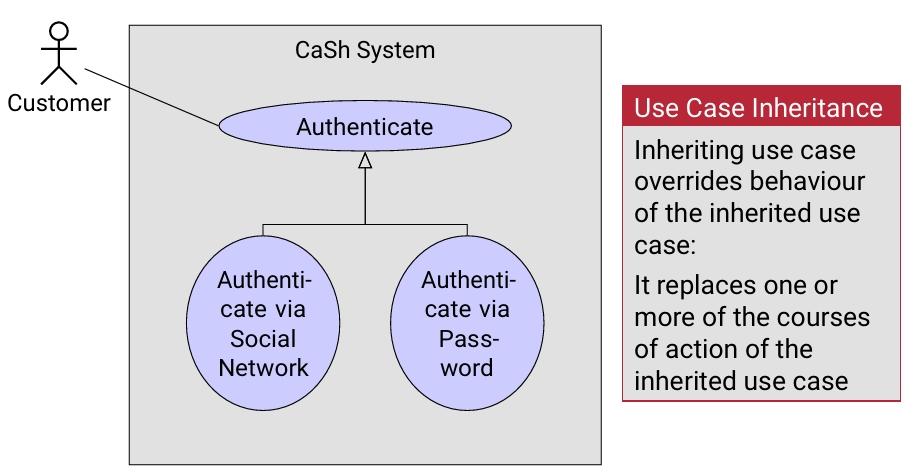
\includegraphics[width=1\textwidth]{Images/UML Use Case Inheritance.jpeg}
\end{figure}

\subsection{Use Cases: Final Remarks}
\begin{defBox}
    Biggest danger: Abusing use cases for system design
\end{defBox}
\begin{itemize}
    \item Use cases are in the \red{problem space.} They document behavioral requirements, \red{use involvement} essential.
    \item Adequate \red{granularity} is important: \red{Elementary business process}, not just a step
    \item \blue{UML use diagrams} most helpful in early use case analysis
    \begin{itemize}
        \item Stay simple, \red{black box} preferred
        \item \red{<<extend>>} breaks encapsulation, use only when justified in UML diagrams 
        \item Never try to anticipate system design with use cases - Don't use \red{inheritance} in UML use case diagrams
        \item Use \red{template}, not diagrams, for fully dressed use case
    \end{itemize}
\end{itemize}
\clearpage
\section{Domain Modelling}
\subsection{Couse Navigation}
\begin{figure}[ht]
    \centering
    \begin{minipage}{0.3\textwidth}
        \centering
        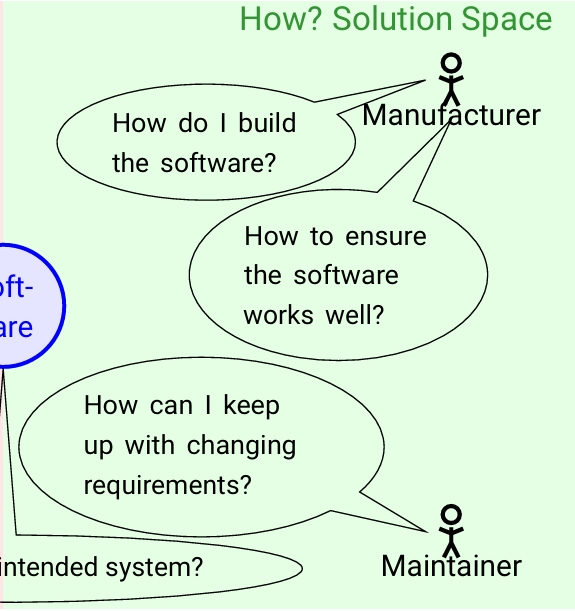
\includegraphics[width=\textwidth]{Images/Course Navigation 1.jpeg}
    \end{minipage}
    \hfill
    \begin{minipage}{0.3\textwidth}
        \centering
        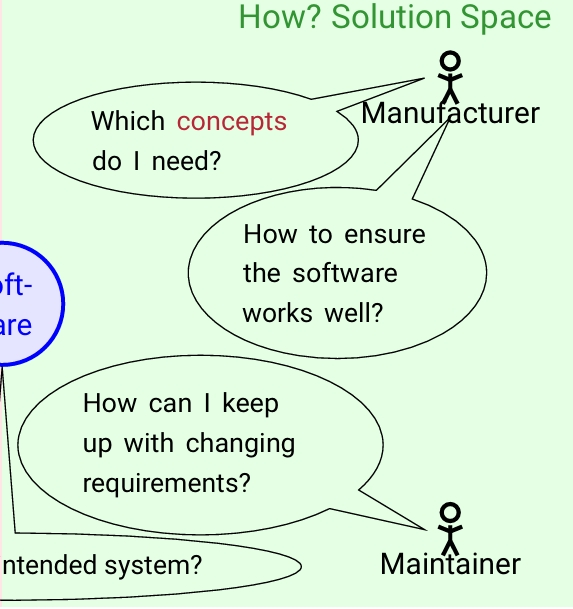
\includegraphics[width=\textwidth]{Images/Course Navigation 2.jpeg}
    \end{minipage}
    \hfill
    \begin{minipage}{0.3\textwidth}
        \centering
        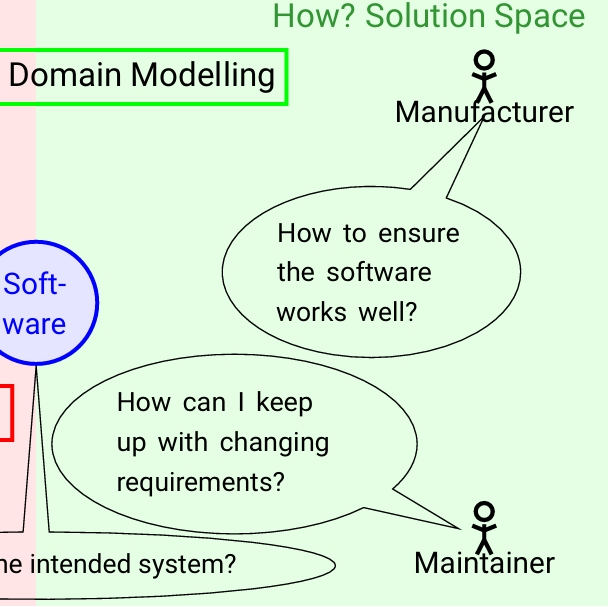
\includegraphics[width=\textwidth]{Images/Course Navigation 3.jpeg}
    \end{minipage}
\end{figure}

\subsection{General Approach: Object-oriented Analysis \& Design}
\begin{defBox}
    In the solution space we use \red{Object-oriented Analysis \& Design} (OOAD)
\end{defBox}
\begin{defBox}[title=Motivation]
    \begin{itemize}
        \item Considered \red{state-of-art}
        \item \red{Widely-used} in industrial practice, many software processes
        \item Numerous \red{training} resources available
        \item Compatible with wide-spread visual modeling notation \red{UML}
        \item Compatible with \red{C++, C\#, JAVA, KOTLIN, SCALA, ...}
    \end{itemize}
\end{defBox}

\subsection{Domain Modelling}
\begin{defBox}[title=Domain Modelling]
    Fixing the \blue{terminology} and \blue{fundamental activities} of the \red{solution space}
    \begin{itemize}
        \item \red{Why:} Helps to identify the \red{relevant} concepts and tasks of a domain
        \item \red{Prerequisite:} \red{Requirements analysis} and \red{use case analysis} are done
        \item \red{Context:} Part of \red{object-oriented analysis} (OOA)
        \item \red{Heuristics:} Only performed for the \red{tasks at hand}
    \end{itemize}
\end{defBox}
\blue{Curtis'law}: \enquote{... good designs require deep application knowledge.}
\begin{defBox}
    Domain model must be \red{validated with \blue{Client}}
\end{defBox}
\begin{infoBox}
    \fatsf{Domain Modeling} beschreibt den Prozess, die Fachterminologie und grundlegende Aktivitäten eines bestimmten Problembereichs (der Domäne) festzulegen und zu strukturieren. Es dient dazu, die relevanten Konzepte und Aufgaben einer Domäne zu indentifizieren und damit die Grundlage für eine lösungsorientierte Systementwicklung zu schaffen.
\end{infoBox}

\begin{infoBox}[title=Warum Domain Modeling?]
    \begin{itemize}
        \item \fatsf{Ziel:} Domain Modeling hilft, die relevanten Konzepte und Aufgaben zu erkennen, die zur Lösung der Anforderungen eines bestimmten Problembereichs nötig sind. Es stellt sicher, dass alle wichtigen Elemente und Interaktionen einer Domäne klar definiert und verstanden sind.
        \item \fatsf{Voraussetzung:} Um ein Domain Model zu erstellen, sollten die \fatsf{Anforderungen} bereits erfasst und durch \fatsf{Use Cases analysiert} worden sein. Das Domain Model baut darauf auf, indem es Konzepte aus diesen Anforderungen abbildet.
    \end{itemize}
\end{infoBox}

\begin{infoBox}[title=Kontext und Ziele des objektorientierten Domain Modeling]
    \begin{itemize}
        \item \fatsf{Teil der Objektorientierten Analyse (OOA):} Somain Modeling ist eng mit der objektorientierten Analyse verbunden und bildet einen Schritt in der objektorientierten Softwareentwicklung.
        \item \fatsf{Curtis'Gesetz:} Ein tiefes Verständnis der Domäne ist notwendig, um gute Entwürfe zu erstellen. Es erfordert daher, dass Entwickler und Fachleute, die das Modell erstellen, die Domäne gut verstehen, um ein realistisches Modell zu entwickeln.
        \item \fatsf{Validierung:} Das Domain Model muss von den Auftraggebern oder Fachexperten validiert werden, um sicherzustellen, dass die erfassten Konzepte korrekt und vollständig sind.
    \end{itemize}
\end{infoBox}
\begin{defBox}[title=Goal of an Object-Oriented Domain Model]
    Decompose the domain into \red{concepts} or \red{objects} that represent the \red{real world} (as captured in the requirements specification)
\end{defBox}
\begin{infoBox}[title=Ziel eines Objektorientierten Domain Models]
    \begin{itemize}
        \item Das Ziel besteht darin, die Domäne in \fatsf{Konzepte oder Objekte} zu unterteilen, die die reale Welt repräsentieren, wie sie in der Anforderungsanalyse dokumentiert wurden.
        \item Dies bildet die Basis für das spätere \fatsf{Softwaredesign}, in dem diese Konzepte als Objekte oder Klassen im Code umgesetzt werden.
    \end{itemize}
\end{infoBox}
\begin{defBox}[title=How to create an Object-Oriented Domain Model]
    \begin{itemize}
        \item Identify the set of \blue{conceptual} \red{classes} and fundamental \red{actions}
    \end{itemize}
    \red{Iteratively} completed and forms the basis for the \red{software design}
\end{defBox}
\begin{infoBox}[title=Erstellung eines objektorientierten Domain Models]
    \begin{itemize}
        \item Die grundlegenden Aktivitäten umfassen das Identifizieren und Definieren der \fatsf{konzeptuellen Klassen} (z.B. Objekte und Entitäten) und \fatsf{fundamentalen Aktionen} (Methoden und Interaktionen), die für die Domäne relevant sind.
        \item Dieser Prozess wird in der Regel iterativ durchgeführt, da das Modell schrittweise vervollständigt und verfeinert wird.
    \end{itemize}
\end{infoBox}
\begin{defBox}[title=Synonyms for Domain Model]
    \begin{itemize}
        \item Conceptual model, domain object model, analysis object model \enquote{\red{Konzeptmodell}}, \enquote{\red{Analysemodell}}
    \end{itemize}
\end{defBox}

\subsection{Conceptual Classes}
\begin{defBox}[title=Conceputal class \enquote{Konzeptklasse}]
    \red{Conceptual classes} represent ideas, things or objects in the domain.\\
    A conceptual class has
    \begin{itemize}
        \item a \red{name} or symbol representing the class,
        \item an \red{intention} (\endquote\red{Bedeutung}),
        \item an \red{extension} (\enquote{\red{Ausprägung}}, \enquote{\red{Extension}}).
    \end{itemize}
    The \red{extansion} \blue{contains} the domain elements the conceptual class represents.
\end{defBox}
\begin{defBox}
    Domain concepts/conceptual classes are \red{not} software objects - They drive from the \red{problem space}
\end{defBox}

\section{UML Class Diagrams}
\subsection{Visualization of Domain Models}
Domain models are visualized using \red{UML class diagrams}\\
\blue{But} with suitable restrictions to emphasize \red{domain} modelling:
\begin{itemize}
    \item Only domain \red{objects} and conceptual \red{classes}
    \item Only \red{associations}, no aggregation, no composition
    \item Classes may have \red{attributes} (used sparingly), but \red{no operations}
\end{itemize}
\begin{defBox}
    UML class diagram of domain model is called \red{conceptual perspective model} \enquote{Modell der Konzeptperspektive}
\end{defBox}
\begin{figure}[h]
    \centering
    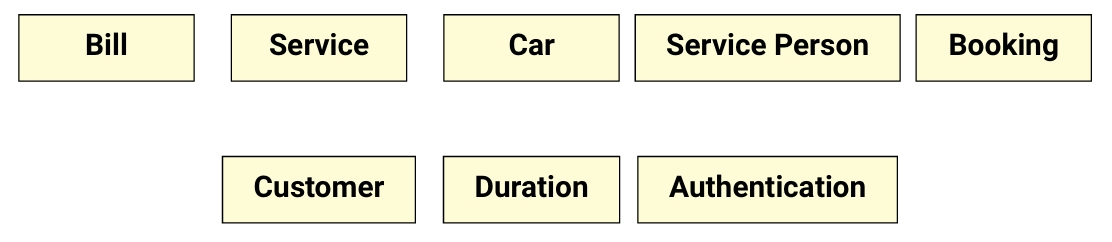
\includegraphics[width=1\textwidth]{Images/CaSh Booking System.jpeg}
\end{figure}
\begin{itemize}
    \item \red{Bookings} are made by \red{customers}
    \item Customers must have \red{authentication} to make a booking
    \item Each booking is for exactly one \red{car}
    \item The monthly \red{bill} comprises all completed and unpaid bookings
    \item Each booking is for a \red{duration} of between 30 minutes and four weeks
    \item A customer connot have more than three active bookings
    \item Each car needs to have a regular \red{service} carried out by a \red{service person}
\end{itemize}
\begin{defBox}[title=Classes]
    A (conceptual) \red{class} describes a set of (domain) objects\\
    An object is an individual thing with a \red{state} and \red{relations} to other objects
\end{defBox}
\subsection{Properties of Conceptual Classes:}
\subsubsection*{Attributes}
\begin{figure}[h]
    \centering
    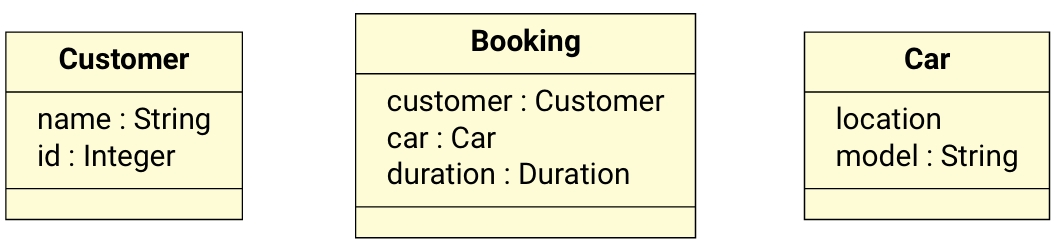
\includegraphics[width=1\textwidth]{Images/Attributes.jpeg}
\end{figure}
\begin{itemize}
    \item Logical data values of an object (class instance, domain element)
    \item Map objects of the containing class to objects of their target type
\end{itemize}
\begin{infoBox}[title=Was sind Attribute?]
    \begin{itemize}
        \item \fatsf{Attribute} sind logische Datenwerte, die eine Klasse und deren Instanzen (also Objekte) näher beschreiben. Sie entsprechen den Informationen, die eine Klasse im System speichert.
        \item Sie stellen eine Abbildung von Objekten der Klasse auf ihre Zielwerte dar. Beispielsweise könnte eine Klasse \fatsf{Person} das Attribut \fatsf{Name} haben, welches Objekte der Klasse \fatsf{Person} auf konkrete Namenswerte (z.B. \enquote{Alice}) abbildet.
    \end{itemize}
\end{infoBox}
During \red{domain modelling:}
\begin{itemize}
    \item Identify attributes of conceptual classes\\
    needed to satisfy \red{information requirements}
    \item \red{Limit} number of attributes to scope of treated scenarios
\end{itemize}
\begin{infoBox}[title=Attribute während der Domänenmodellierung]
    \begin{enumerate}
        \item \fatsf{Identifizierung der benötigten Attribute:}
        \begin{itemize}
            \item In der Phase der Domänenmodellierung ist es wichtig, Attribute nur dann zu definieren, wenn sie tatsächlich zur Erstellung der Informationsanforderungen relevant sind. Beispielsweise könnte ein Attribut \fatsf{Adresse} für die Klasse \fatsf{Kunde} nur dann notwendig siein, wenn Adressinformationen für die Geschäftprozesse erforderlich sind.
        \end{itemize}
        \item \fatsf{Begrenzung auf szenario-relevante Attribute:}
        \begin{itemize}
            \item Es ist ratsam, die Anzahl der Attribute auf das Wesentlich zu beschränken, um die Modellkomplexität zu verringern. Attribute sollten daher nur die Informationen abdecken, die für die im Modell behandelten Szenarien erforderlich sind.
        \end{itemize}
        \item \fatsf{Begrenzung auf szenario-relevante Attribute:}
        \begin{itemize}
            \item Es ist ratsam, die Anzahl der Attribute auf das Wesentliche zu beschränken, um die Modellkomplexität zu verringern. Attribute sollten daher nur die Informationen abdecken, die für die im Modell behandelten Szenarien erforderlich sind.
        \end{itemize}
    \end{enumerate}
\end{infoBox}
\subsection{UML Model Element Class: Simplified Syntax for Domain Modelling}
\begin{figure}[h]
    \centering
    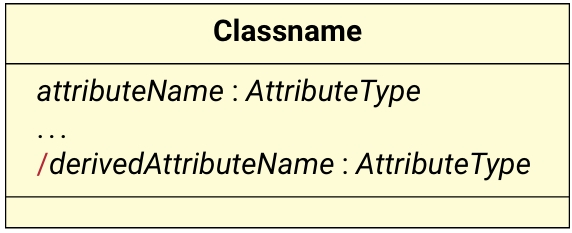
\includegraphics[width=0.5\textwidth]{Images/Class.jpeg}
\end{figure}

\begin{defBox}[title=UML Class Elements and Conventions]
    \begin{itemize}
        \item \red{Class Name:} Class names start always with an upper case letter
        \item \red{Attribute:} \blue{Attribute name:} starts with a lower case letter\\
        \blue{Attribute type:} pre-defined type or other domain model class (type can be \red{omitted} in domain modelling)
        \begin{infoBox}
            In der Phase der Domänenmodellierung ist es nicht zwingend erforderlich, den Typ jedes Attributes anzugeben. Oft genügt es, das Attribut selbst zu identifizieren, um den Zweck des Modells klar darzustellen.
        \end{infoBox}
        \item \red{Derived Attribute:} name prefixed by a slash ('\red{\textbackslash}')\\
        Value computable from existing infomration
    \end{itemize}
\end{defBox}
\begin{infoBox}[title=Abgeleitet Attriubte]
    \begin{itemize}
        \item Ein \fatsf{abgeleitetes Attribut} ist ein Attribut, dessen Wert aus anderen vorhandenen Informationen berechnet werden kann. Solche Attribute werden mit einem Schrägstrich (/) vor dem Namen gekennzeichnet.
        \item \fatsf{Beispiel:} Ein Attribut \fatsf{/Gesamtpreis} in der Klasse \fatsf{Rechnung} könnte als Summe der einzelnen Positionen berechnet werden, anstatt separat gespeichert zu werden.\\
        \fatsf{Notation:} /Gesamtpreis zeigt an, dass dieses Attribut nicht manuell eingegeben wird, sondern als Ergebnis einer Berechnung oder Ableitung verfügbar ist.
    \end{itemize}
\end{infoBox}

\subsection{Example: Derived Attribute}
\begin{figure}[h]
    \centering
    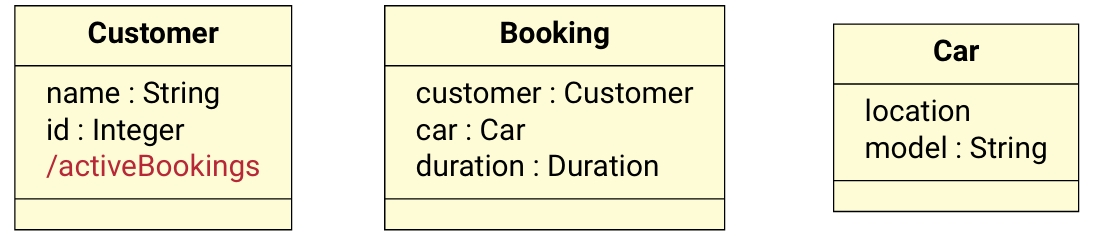
\includegraphics[width=1\textwidth]{Images/Derived Attribute.jpeg}
\end{figure}
\begin{defBox}[title=Example (Active Boodings)]
    \begin{itemize}
        \item The \red{active bookings} of a customer are all not yet completed bookings
    \end{itemize}
    The active bookings for a customer can be computed:\\
    \blue{Collect all bookings of the customer whose end time is not past the current time}\\
    Derived attributes are usually not assigned values independently
\end{defBox}

\subsection{CaSh Booking System: Associations (Relations)}
\begin{figure}[h]
    \centering
    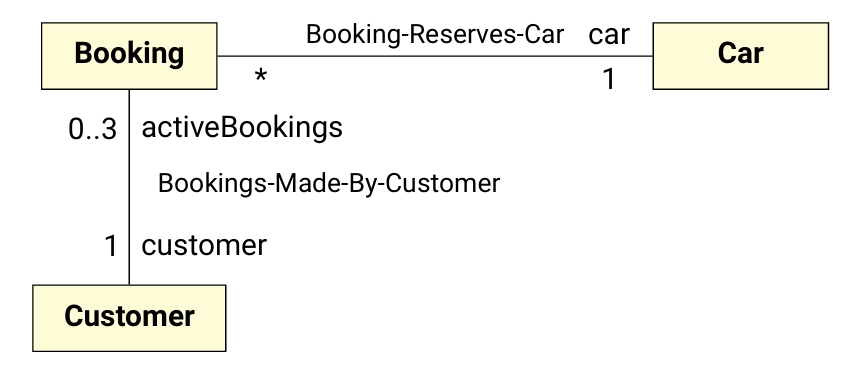
\includegraphics[width=1\textwidth]{Images/Associations (Relations).jpeg}
\end{figure}
\begin{itemize}
    \item \red{Bookings} are made by \red{customers}
    \item A customer cannot have more than \red{three} active bookings
    \item Each booking is for \red{exactly} one car
    \item A car may appear in an arbitrary number of bookings
\end{itemize}

\clearpage
\subsection{Syntax of UML Association}
\begin{figure}[h]
    \centering
    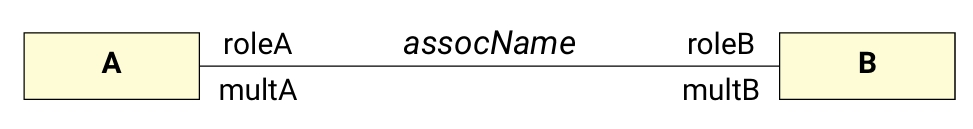
\includegraphics[width=1\textwidth]{Images/Syntax of UML Asociation.jpeg}
\end{figure}
\blue{An} \red{association} \blue{is a relation among classes with the elements:}
\begin{itemize}
    \item Name (optional)
    \item Two association ends called \red{roles}, each with:
    \begin{itemize}
        \item A \red{role name} (defaults to class name starting with lower case letter)
        \item A \red{multiplicity} (defaults to multiplicity 1)\\
        Possible multiplicities: * or a ..b\\
        a, b are \red{value specifications} (numbers expressions); upper bound incl. *
        \item A \red{navigability} (defaults to bi-directional, not used for conceptual classes)
    \end{itemize}
\end{itemize}
\begin{figure}[h]
    \centering
    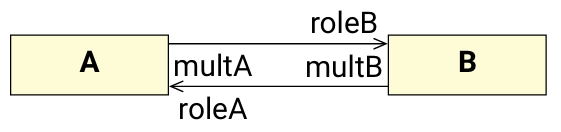
\includegraphics[width=0.5\textwidth]{Images/navigability.jpeg}
\end{figure}

\subsection{Generalizations of Concepts}
\begin{figure}[h]
    \centering
    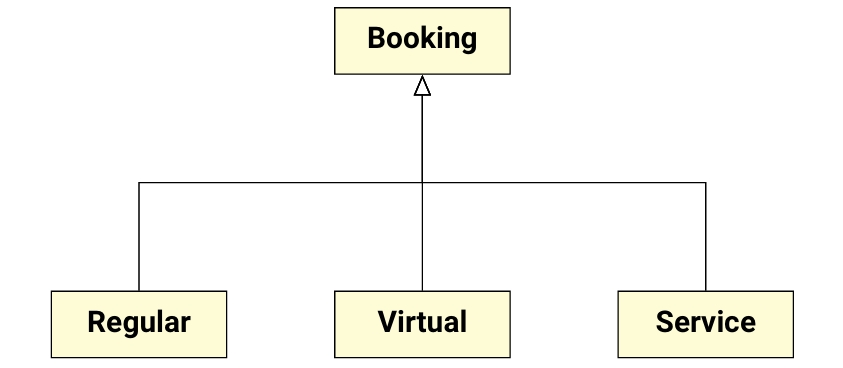
\includegraphics[width=0.5\textwidth]{Images/Generalizations of Concepts.jpeg}
\end{figure}
\begin{itemize}
    \item There are different types of bookings: regular, virtual, service
\end{itemize}

\subsection{Elicitation of Domain Model for a New Domain: Workflow}
\begin{enumerate}
    \item Find the \red{conceptual classes}\\
    Strategies:
    \begin{itemize}
        \item \red{Re-use} or modify an existing model
        \item Use a category \red{list}
        \item Identify \red{noun phrases}
    \end{itemize}
    \item Draw elicited concepts as a classes in a UML class diagram
    \item Add \red{attributes}
    \item Add \red{associations}
\end{enumerate}
\begin{defBox}
    Use the domain vocabulary: The CaSh model should use names like \red{Customer} instead of \blue{Person}
\end{defBox}
\begin{infoBox}
    Die \fatsf{Erhebung (Elicitation) eines Domain Models für eine neue Domäne} ist ein strukturierter Prozess bei dem relevante Konzepte und Beziehungen identifiziert und in ein Modell übertragen werden. Die folgende Übersicht beschreibt die einzelnen Schritte dieses Workflows:
\end{infoBox}
\begin{infoBox}[title=Workflow zur Erstellung eines Domain Models]
    \begin{enumerate}
        \item \fatsf{Konzeptuelle Klassen finden}\\
        Die Konzeptklassen sind die grundlegende Bausteine des Domain Models. Sie repräsentieren wichtige Objekte oder Entitäten in der Domäne, z.B. \enquote{Kunde} oder \enquote{Produkt}. Es gibt mehrere Strategien, um diese Klasse zu identifizieren:
        \begin{itemize}
            \item \fatsf{Vorhandenes Modell wiederverwenden oder anpassen:} Prüfen, ob es bereits ein ähnliches Modell gibt, das an die aktuelle Domäne angepasst werden kann.
            \item \fatsf{Kategorie-Liste verwenden:} Eine Liste typischer Kategorien wie \enquote{Personen}, \enquote{Objekte}, \enquote{Orte} oder \enquote{Transaktionen} kann helfen, wichtige Konzepte zu finden.
            \item \fatsf{Substantivphasen identifizieren:} In den Anforderungen nach Substantiven suchen, die Konzepte darstellen könnten (z.B. \enquote{Kunde}, \enquote{Termin}).
        \end{itemize}
        \item \fatsf{Konzepte als Klassen in einem UML-Klassendiagramm darstellen}
        \begin{itemize}
            \item Die identifizierten Konzeptklassen werden nun in einem \fatsf{UML-Klassendiagramm} als einzelne Klassen mit Namen dargestellt
            \item Dieses Diagramm hilft, die Konzepte zu visualisieren und zeigt, wie sie in Beziehung zueinander stehen könnten.
        \end{itemize}
        \item \fatsf{Attribute hinzufügen}
        \begin{itemize}
            \item In jedem Konzept wird überlegt, welche spezifischen \fatsf{Eigenschaften oder Merkmale (Attribute)} erforderlich sind.
            \item Zum Beispiel könnte die Klasse \enquote{Kunde} Attribute wie \enquote{Kundenname} und \enquote{Kundennummer} haben.
        \end{itemize}
        \item \fatsf{Assoziationen hinzufügen}
        \begin{itemize}
            \item Assoziationen zeigen die \fatsf{Beziehungen zwischen den Klassen}. Diese Beziehungen geben Einblick in die Interaktionen zwischen den Konzepten und wie sie zusammenarbeiten.
            \item Zum Beispiel könnte eine Assoziation zwischen den Klassen \enquote{Kunde} und \enquote{Bestellung} die Beziehung \enquote{Kunde erstellt Bestellung} darstellen.
        \end{itemize}
    \end{enumerate}
\end{infoBox}

\clearpage
\subsection{Re-using an Existing Model}
\begin{figure}[h]
    \centering
    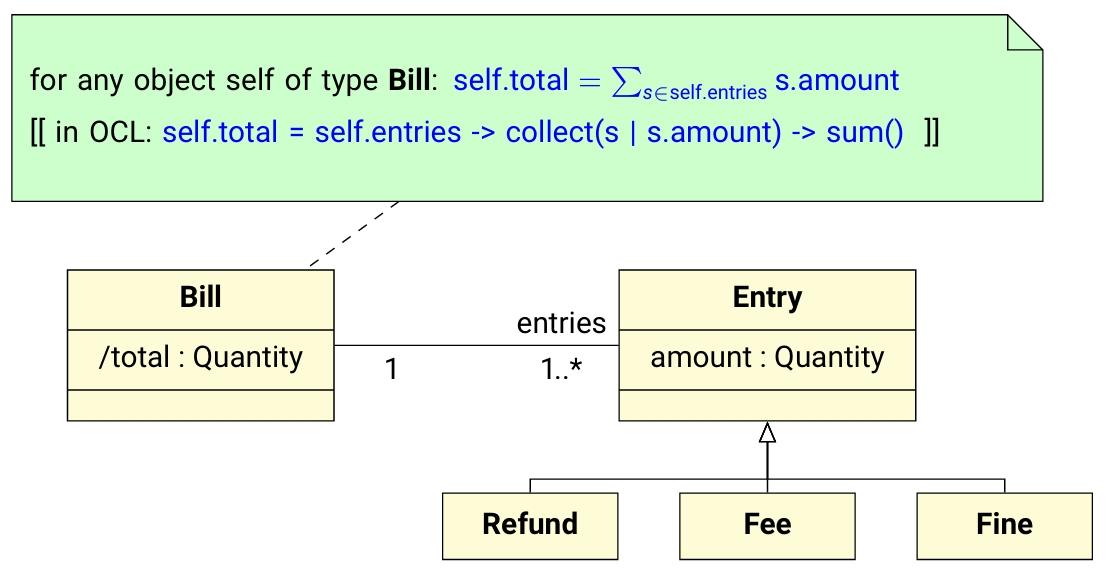
\includegraphics[width=1\textwidth]{Images/Re-using an Existing Model.jpeg}
\end{figure}
\begin{infoBox}[title=UML-Diagramm und Beziehungen]
    Das UML-Diagramm zeigt zwei zentrale Klassen und ihre Attribute:
    \begin{itemize}
        \item \fatsf{Bill:} Repräsentiert eine Rechnung, die das Attribut \textbackslash total hat. Das \textbackslash vor dem Attributnamen weist darauf hin, dass es ein berechnetes Attribut ist.
        \item \fatsf{Entry:} Repräsentiert einen einzelnen Eintrag auf der Rechnung mit dem Attribut \fatsf{amount}, das den Betrag des Eintrags speichert
        \item \fatsf{Assoziationen:}
        \begin{itemize}
            \item \fatsf{eintries:} Eine \enquote{Bill} enthält eine oder mehrere \enquote{Entry}-Objekte (dargestellt durch die Kardinalität \enquote{1..*}). Diese Beziehung zeigt, dass jede Rechnung eine Liste von Einträgen hat, und jeder Eintrag gehört genau zu einer Rechnung.
        \end{itemize}
    \end{itemize}
    Zusätzliche Klassen wie \fatsf{Refund, Fee} und \fatsf{Fine} sind spezialisierte Typen von Entry. Diese Subklassen könnten spezifische Arten von Einträgen darstellen, z.B. \enquote{Erstattung} (Refund), \enquote{Gebühr} (Fee) oder \enquote{Strafe} (Fine).
\end{infoBox}
\subsection{Identification of Concept Classes: List of Conceptual Class Categories}
\begin{defBox}[title=Some Categories]
    \begin{itemize}
        \item Physical or tangible objects
        \item Specifications or description of things
        \item Locations
        \item Events
        \item Transactions
        \item Transaction items
        \item Organizations
        \item Roles (of people, organizations, etc.)
        \item Containers
        \item ...
    \end{itemize}
\end{defBox}
\subsection{Using a Category: Example}
\begin{table}[H]
    \centering
    \rowcolors{2}{\thepagecolor}{fgcolor!10!\thepagecolor}
    \renewcommand{\arraystretch}{1.2}
    \begin{tabular}{lll}
        \toprule
        Conceptual Class Category & Conceptual Classes (in CaSh) \\
        \midrule
        Business transaction & Bill, Payment\\
        Transaction line item & Entry\\
        Product or service related to a transaction or to a transaction line item & Refund, Rent, Fine\\
        Place where transaction is recorded & Registry\\
        Roles of people or organizations related to a transaction (actors in use cases) & Customer, Accountant\\
        Location where transaction executed & Website\\
        Noteworthy events, with a time or place that needs to be remembered & Bill, Booking\\
        \bottomrule
    \end{tabular}
\end{table}
\begin{infoBox}[title=Kategorien konzeptioneller Klassen]
    \begin{enumerate}
        \item \fatsf{Physische oder greifbare Objekte}
        \begin{itemize}
            \item Beziehen sich auf reale, konkrete Objekte.
            \item \fatsf{Beispiele:} Geräte, Fahrzeuge, Produkte.
        \end{itemize}
        \item \fatsf{Spezifikationen oder Beschreibungen von Objekten}
        \begin{itemize}
            \item Dienen zur detaillierten Beschreibung von Dingen, die wichtig für das System sind.
            \item \fatsf{Beispiele:} Produktbeschreibungen, Service-Beschreibungen, Mietobjektbeschreibungen.
        \end{itemize}
        \item \fatsf{Orte (Locations)}
        \begin{itemize}
            \item Definieren spezifische physische oder virtuelle Orte, die in den Prozessen des Systems relevant sind.
            \item \fatsf{Beispiele:} Lagerorte, Abteilungen, virtuelle Plattformen.
        \end{itemize}
        \item \fatsf{Ereignisse (Events)}
        \begin{itemize}
            \item Ereignisse oder Aktionen, die in einem bestimmten Zeitrahmen stattfinden und verfolgt werden müssen.
            \item \fatsf{Beispiele:} Termine, Registrierungen, Alarmmeldungen.
        \end{itemize}
        \item \fatsf{Transaktionen}
        \begin{itemize}
            \item Beschreiben eine Art von Geschäftsprozessen oder Austauschvorgängen, die vom System unterstützt werden.
            \item \fatsf{Beispiele:} Bestellungen, Zahlungen, Buchungen.
        \end{itemize}
        \item \fatsf{Transaktionsposten (Transaction Items)}
        \begin{itemize}
            \item Einzelne Einträge innerhalb einer größeren Transaktion, die oft wiederholt oder in Kombination vorkommen.
            \item \fatsf{Beispiele:} Rechnungsposten, Produktpositionen in einer Bestellung.
        \end{itemize}
        \item \fatsf{Organisationen}
        \begin{itemize}
            \item Unternehmensstrukturen oder andere Organisationen, die eine Rolle im System spielen.
            \item \fatsf{Beispiele:} Lieferanten, Partnerunternehmen, Abteilungen.
        \end{itemize}
        \item \fatsf{Rollen (Roles)}
        \begin{itemize}
            \item Rollen, die von Personen oder Organisationen eingenommen werden und in den Anwendungsfällen eine spezifische Bedeutung haben.
            \item \fatsf{Beispiele:} Kunden, Administratoren, Verkäufer.
        \end{itemize}
        \item \fatsf{Container}
        \begin{itemize}
            \item Strukturen, die mehrere Elemente zusammenfassen und gruppieren, um Beziehungen oder organisatorische Strukturen widerzuspielgeln.
            \item \fatsf{Beispiele:} Ordner, Sammlungen, Inventarcontainer.
        \end{itemize}
        \item \fatsf{Weitere Kategorien}
        \begin{itemize}
            \item Abhängig von der spezifischen Domäne können zusätzliche Kategorien wie \fatsf{Dokumente}, \fatsf{Protokolle}, oder \fatsf{Metriken} sinnvoll sein.
        \end{itemize}
    \end{enumerate}
\end{infoBox}


\subsection{Conceptual Class Discovery Technique: Noun Identification}
\begin{defBox}[title=Workflow]
    \begin{itemize}
        \item Identify \red{nouns} and noun phrases in textual descriptions of domain
        \item Consider them as a \red{condidate} for a conceptual class or an attribute
    \end{itemize}
\end{defBox}
\blue{Can it be automated?}\\
Only \red{patially}: Words in natural language texts are \red{ambiguous}
\begin{itemize}
    \item Same noun can mean multiple things
    \item Different nouns can mean the same thing
\end{itemize}
\begin{defBox}
    \red{Use Cases} (stories) are a canonical sorce for identifying conceptual classes
\end{defBox}

\subsection{Example: Noun Identification}
\begin{defBox}[title=Text Story: Change Existing Booking]
    The \red{customer} selects the \red{booking} to change. The \red{system} displays the booking \red{details}, including adjacent \red{reservations}. The customer is offered to change the reserved \red{duration}. Whin a new duration is entered, the system checks \red{availability} and records the \red{change}. In case of no availability, nothing happens and an \red{information message} is displayed. Before any change happens, a \red{confirmation action} is requested. Afterwards, a \red{confirmation message} is sent to the customer's preferred \red{contact}.
\end{defBox}
\begin{defBox}[title=Condidate Conceptual Classes]
    Customer, Booking, Detail, Reservation, Duration, System, Availability, Change, InformationMessage, ConfirmationAction, ConfirmationMessage, Contact
\end{defBox}

\subsection{Selection of Suitable Conceputual Classes}
\begin{defBox}
    Which nouns should become conceptual classes in domain model?
\end{defBox}
\blue{Example: Should} \red{ConfirmationMessage} \blue{be a conceptual class?}
\begin{defBox}[title=Criteria to include a candidate conceptual class:]
    \begin{itemize}
        \item Must \red{carry information} not available/computable from other sources\\
        \red{Avoid} candidates that add only
        \begin{itemize}
            \item redundant information (available elsewhere)
            \item derived information
        \end{itemize}
        \item Must have specific semantics in relation to the \red{besiness}
    \end{itemize}
\end{defBox}
\blue{What does that mean for} \red{ConfirmationMessage} ?
\begin{itemize}
    \item A \red{confiramtion message} repeats content from changed booking
\end{itemize}
\blue{Conclusion:} \red{Confirmation Message} is \red{report} about a booking

\subsection{Boundary of Domain Model}
\red{Report:} \blue{Part of the domain model? - It depends!}
\begin{itemize}
    \item Considering \red{current} scenario only:\\
    $\Rightarrow$ Confirmation message \red{not} part of domain model (only a report)
    \item Considering, for example, handling of disputes:\\
    $\Rightarrow$ Confirmation message represents an important \red{concept on its own}
\end{itemize}
\blue{In general:}
Regarding legal aspects ...? $\leftarrow$ Non-functional \red{domain requirement}
\begin{infoBox}
    Um zu entscheiden, ob ein Konzept wie die Bestätigungsnachricht Teil des Domänenmodells sein sollte:
    \begin{itemize}
        \item Prüfen, ob es neue Informationen liefert oder eine spezifische Rolle hat.
        \item Aktuelle und mögliche zukünftige Anwendungsfälle berücksichtigen (z.B. Streitfallbearbeitung).
        \item Eventuelle rechtliche oder regulatorische Anforderungen evaluieren, die die Notwendigkeit einer konzeptuellen Klasse beeinflussen könnten.
    \end{itemize}
\end{infoBox}

\subsection{More In-/Exclusion Criteria for Conceptual Classes}
\begin{defBox}[title=Candidate Conceptual Classes]
    Customer, Booking, Detail, Reservation, Duration, System, Availability, Change, InformationMessage, ConfirmationMessage, ConfirmationAction, Contact
\end{defBox}
\begin{enumerate}
    \item Customer, Booking, Duration, ConfirmationMessage: Already used, discussed
    \item Detail: Summary expression actually referring to \red{Car}, \red{Duration}, ...
    \item Reservation: Synonym of \red{Booking}
    \item System: Root class, not a specific concept
    \item Availability: Derivable from \red{Duration} and bookings
    \item Change: Synonym of changed \red{Booking}
    \item ...
\end{enumerate}

\subsection{Description Classes}
\begin{defBox}
    A \red{description class} contains information that describes an entitiy
\end{defBox}
\begin{defBox}[title=Example]
    \begin{itemize}
        \item A rental location description has information on : Address, accessiblity, closest public transpoert, etc.
    \end{itemize}
\end{defBox}
A description class should be \red{added} to the domain model  in these cases:
\begin{enumerate}
    \item Information about an item or service is required, \blue{regardless of whether any instance of those items or services exist}
    \item Dleting icstances of described entities results in \blue{loss of information}
    \item \blue{Redundant} or duplicated infomrmation is reduced
\end{enumerate}
\subsection{Model a Notion as Class or Attribute?}
\begin{defBox}[title=Heuristics: Class or Attribute]
    If we \red{do not think} of a notion C as a number, text or date of the real world, then C is probably a conceptual class, not an attribute
\end{defBox}
\begin{defBox}[title=Example (Airport)]
    \begin{itemize}
        \item Should \red{destination} be an attribute of flight, or a conceptual class airport?
        \item Name of airport?
    \end{itemize}
\end{defBox}
\begin{figure}[h]
    \centering
    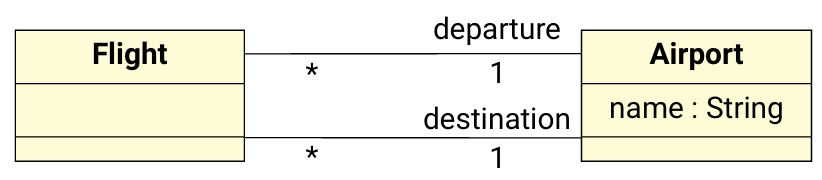
\includegraphics[width=1\textwidth]{Images/Example (Airport).jpeg}
\end{figure}

\subsection{Use of Associations in Domain Modelling}
\begin{defBox}[title=Heuristics]
    Include associations in the domain model when: \blue{Knowledge about the relation needs to be preserved for some time}
\end{defBox}
\begin{defBox}[title=Example]
    The relation between a \red{bill} and its \red{entries} needs to be remembered\\
    But it is unnecessary to store the relation between a customer and his or her most recent search for available cars\\
    On the other hand, a \red{browser} might well redcord the search history
\end{defBox}
List of common association \red{categories}:
\begin{itemize}
    \item A is a \red{transaction} related to another transacton B
    \item A is a \red{line item} of a transaction B
    \item A is a \red{product} or a \red{service} for a transaction B
    \item A is a \red{role} related to a transaction B
    \item A is a physical or logical \red{part} of B
\end{itemize}

\subsection{Association Name}
\begin{defBox}
    Name an association based on a \red{Class name-Verb phrase-Class name} format\\
    The verb phrase creates a sequence that is readable and meaningful
\end{defBox}
\blue{Good examples:}
\begin{itemize}
    \item Player \blue{Stands-on-} Square
    \item Sale-\blue{Paid-by}-CashPayment
\end{itemize}
\red{Bad examples:}
\begin{itemize}
    \item Player-\red{Has}-Square (\enquote{Has} is generic, doesn't tell about relation)
    \item Sale-\red{Uses}-CashPayment (\enquote{Uses} dito)
\end{itemize}

\subsection{Attribute or Association?}
\begin{defBox}
    A \red{property} can be modelled as an \red{association} or an \red{attribute}
\end{defBox}
\blue{The notations are very different! - When to use what?}
\begin{itemize}
    \item Attributes should always be used for \red{primitive} datatypes
    \begin{itemize}
        \item Boolean, Integer, Character, String
        \item Date, Address, Color, Phone Number, ...
    \end{itemize}
    \item Quantities \red{may} be modelled as classes to attach units
    \begin{itemize}
        \item currency (EUR, USD, SEK, ...)
        \item weight (kilogram, cm, ...)
    \end{itemize}
    \item \red{Always} use associations to model relations between conceptual classes
\end{itemize}
\begin{figure}[h]
    \centering
    \includegraphics[width=1\textwidth]{Images/Attribute or Association?.jpeg}
\end{figure}

\subsection{Refining a Model: Replace String Type}
\begin{defBox}
    It is convenient to type attributes \red{initially} with \blue{String}:\\
    \red{Generic} type that avoids \red{premature} decision\\
    Later, consider \red{refinement} to description class
\end{defBox}
\begin{figure}[h]
    \centering
    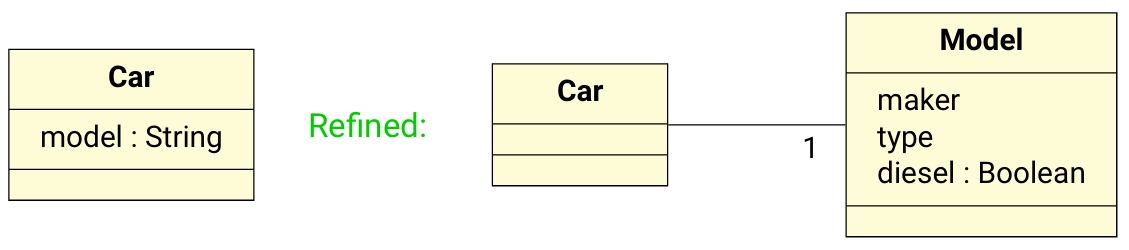
\includegraphics[width=1\textwidth]{Images/Refining a Model.jpeg}
\end{figure}
\begin{itemize}
    \item When string has \red{structure}, i.e. composed of separate sections: Maker, type
    \item When other \red{relations} are associated with the string: social security nr
    \item When the string has other \red{attributes}: diesel
    \item When the string is a quantity with a \red{unit}, for example, a currency
\end{itemize}

\subsection{CaSh Booking System: Domain Model (Excerpt)}
\begin{figure}[h]
    \centering
    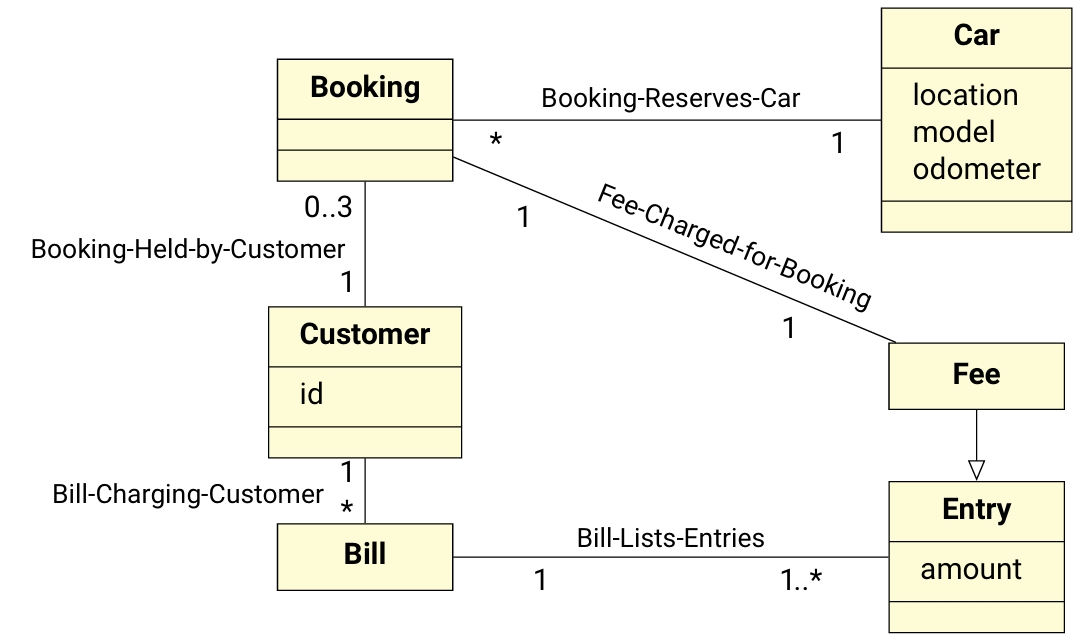
\includegraphics[width=1\textwidth]{Images/Domain Model (Excerpt).jpeg}
\end{figure}

\clearpage
\subsection{From Domain Model to Design model}
\begin{defBox}
    The domain model serves as a source of \red{inspiration} for the design model
\end{defBox}
\begin{figure}[h]
    \centering
    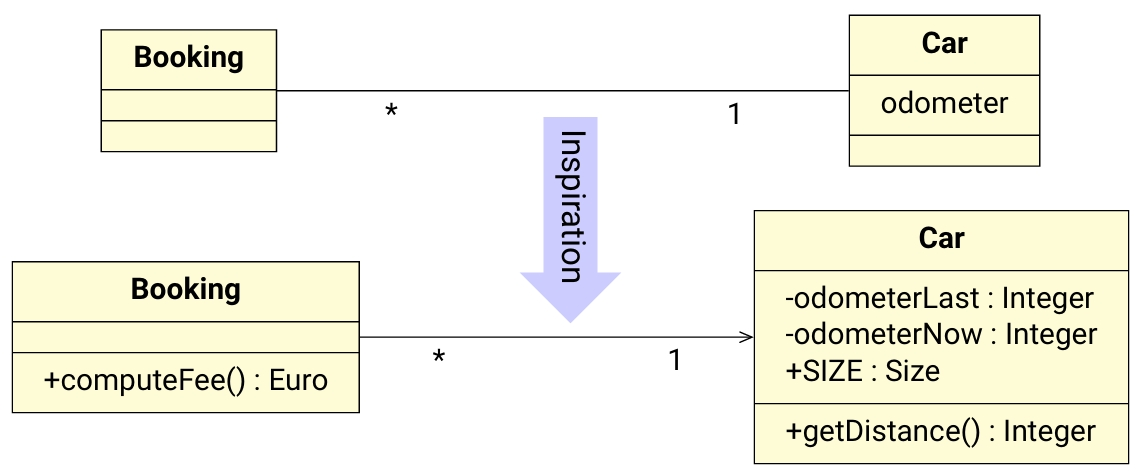
\includegraphics[width=1\textwidth]{Images/From Domain Model to Design Model.jpeg}
\end{figure}

\subsection{Domain Model is Not Static View on Code}
\begin{defBox}[title=The Two Faces of UML Class Diagrams]
    \begin{itemize}
        \item \red{Conceptual perspective model} in domain modelling (our usage)
        \item Static view (classes, methods, fields) extracted from \red{OO code}
    \end{itemize}
\end{defBox}
\begin{defBox}
    Don't confuse them, for example, abuse the former as code stubs
\end{defBox}

\section{Behavioral Models}
\subsection{Behavioral Domain Modelling}
\begin{defBox}
    Class diagrams model \red{static} aspects of software
\end{defBox}
\begin{itemize}
    \item Classes, objects
    \item Properties: attributes, associations
    \item Functions
\end{itemize}
\begin{defBox}
    What about \red{behavior}?
\end{defBox}
\begin{itemize}
    \item \red{Sequences of actions} and how they change the
    \begin{itemize}
        \item \red{state of a system}
        \item under which \red{condition}
    \end{itemize}
\end{itemize}

\subsection{UML State Machine Diagrams}
\begin{defBox}
    \red{UML State Machine Diagrams} are finite state machines whose transitions are equipped with \red{in-/output actions} and \red{guards}
\end{defBox}
\begin{figure}[h]
    \centering
    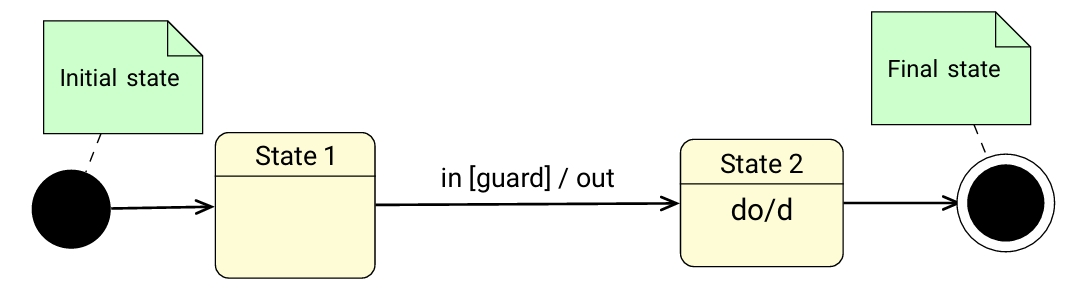
\includegraphics[width=1\textwidth]{Images/UML State Machine Diagrams.jpeg}
\end{figure}

\begin{defBox}[title=Semantics]
    When in \red{State 1}, if \red{input} in is observed and \red{guard} is true, then \red{output} out happens and current state becomes \red{State 2}.\\
    In \red{State 2} perform (interruptible) \red{action} d.
\end{defBox}

\subsection{Basic States}
\begin{figure}[h]
    \centering
    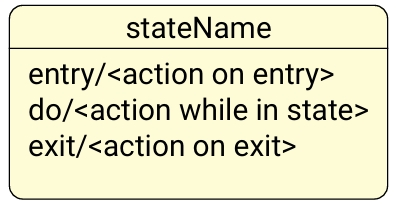
\includegraphics[width=0.5\textwidth]{Images/Basic States.jpeg}
\end{figure}
\begin{defBox}[title=Basic States in Detail]
    \begin{itemize}
        \item Basic states have a \red{name} and can define any combination of 
        \begin{itemize}
            \item \red{entry action:} action performed on state entry
            \item \red{do action:} action performed while in state (until the action terminates or the state is left)
            \item \red{exit action:} action performed on state exit
        \end{itemize}
        \item Actions are executed \red{operations}
    \end{itemize}
\end{defBox}

\clearpage
\subsection{Basic States: INitial, Final \& Terminal States}
\begin{figure}[h]
    \centering
    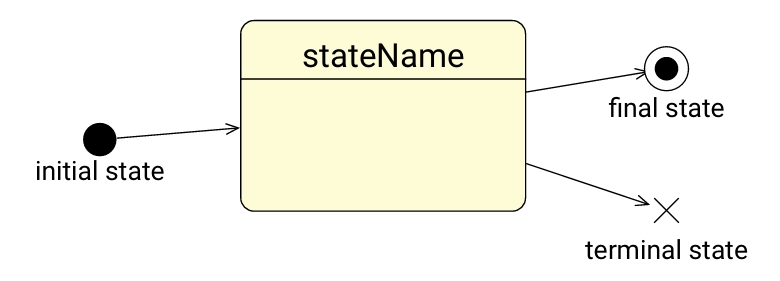
\includegraphics[width=0.5\textwidth]{Images/Initial, Final und Terminal States.jpeg}
\end{figure}
\begin{defBox}[title=States with Special Meaning]
    \begin{itemize}
        \item \red{Inital State:} has single transition to \red{first} entered state (may be labeled by object creation event/message)
        \item \red{Final State:} indicates completion of scenario
        \item \red{Terminal State:} completion and executing object destroyed
    \end{itemize}
\end{defBox}

\subsection{Transitions between States}
\begin{figure}[h]
    \centering
    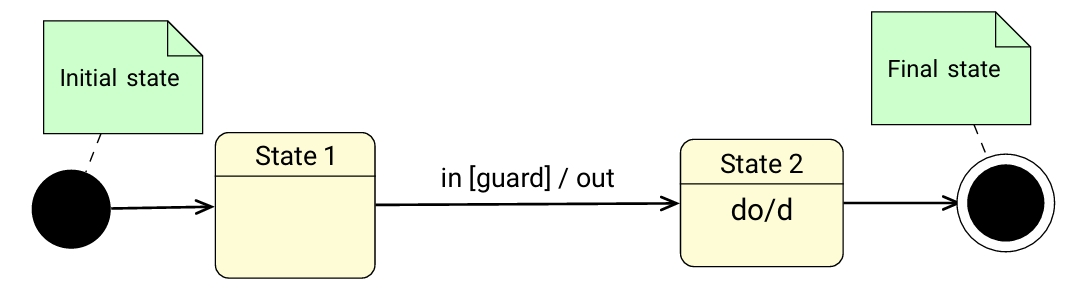
\includegraphics[width=1\textwidth]{Images/UML State Machine Diagrams.jpeg}
\end{figure}
\begin{defBox}[title=Transition Labels: input? ('[' guard ']')? '/' output?]
    \begin{itemize}
        \item All parts are optional (indicated by ?)
        \item \red{Input} (trigger) events are observations such as:
        \begin{itemize}
            \item call event (start of operation)
            \item time event (for example, time spent in a state)
            \item change event (value of an attribute has changed)
        \end{itemize}
        \item \red{gaurd} is a Boolean expression
        \item \red{Output} (action) is an operation or domain-specific action expression
    \end{itemize}
\end{defBox}

\clearpage
\subsection{State Machine Diagram: Example (Credit Card Payment with PIN)}
\begin{figure}[h]
    \centering
    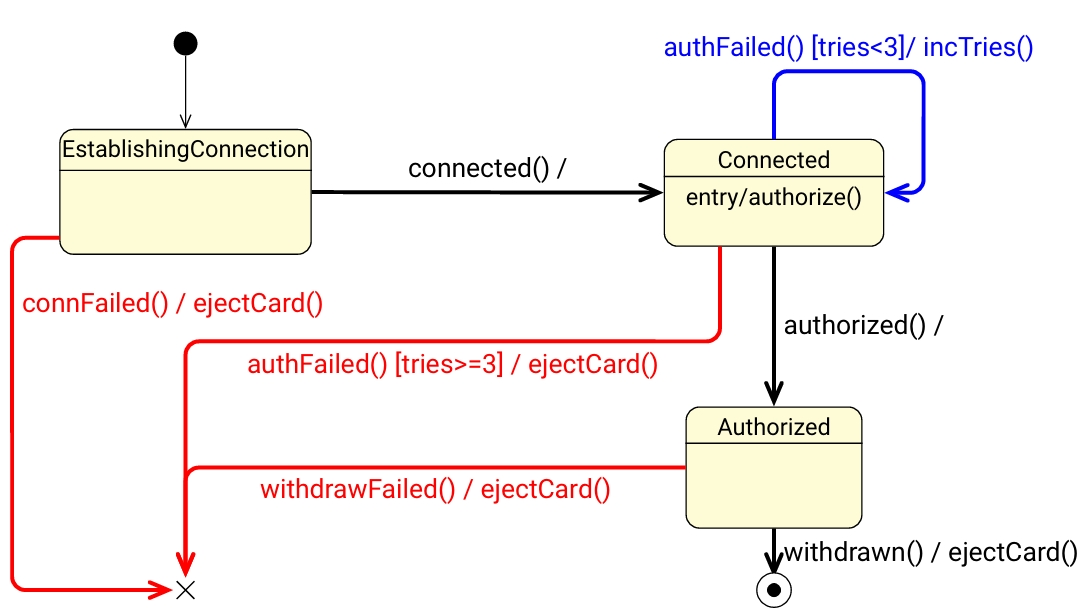
\includegraphics[width=1\textwidth]{Images/State Machine Diagram.jpeg}
\end{figure}

\subsection{State Machine Diagrams in Domain Modelling}
\begin{defBox}
    During domain modelling: State machine diagrams \red{do not relate to code}
\end{defBox}
\begin{defBox}[title=Uses of State Machine Diagrams in Doamin Modelling]
    \begin{itemize}
        \item Capture the action sequence of a \red{use case}
        \item \red{Combine} several, related use cases
        \item Clarify the \red{states} an object can be in
        \item Help to clarify \red{protocols}
        \item Help to \red{validate} the domain model
        \item Help to \red{complete} the domain model (with properties / actions)
    \end{itemize}
    State machine diagrams should only be used to model \red{non-trivial behavior}
\end{defBox}
\clearpage
\section{Software Architecture}
\subsection{What? How?}
\begin{figure}[h]
    \centering
    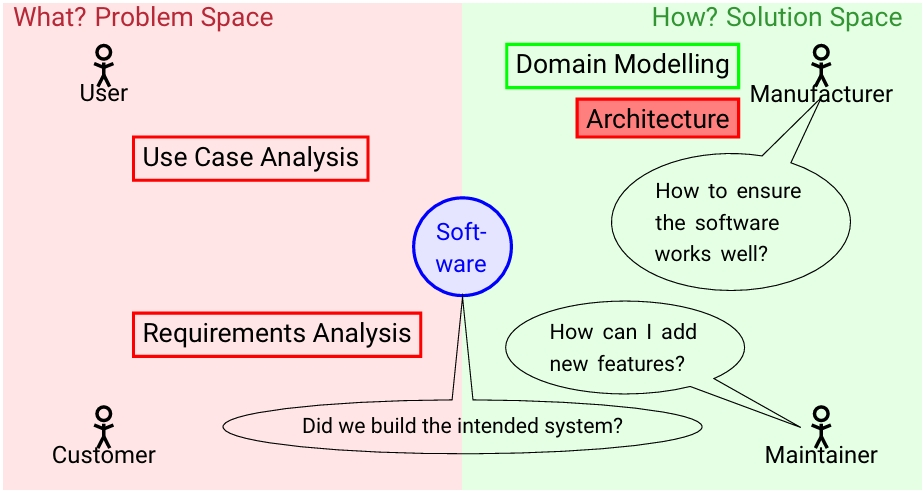
\includegraphics[width=1\textwidth]{Images/Architecture.jpeg}
\end{figure}

\subsubsection*{A Product of its Time}
\begin{defBox}
    Software architecture is a fast evolving area in software engineering
\end{defBox}
Architectures \red{favoured in the past} are \red{now discouraged}\\
\& Architecture \red{discouraged in the past} are \red{now preferred}\\
Changes in the last 10 to 15 years that influenced architecture:
\begin{itemize}
    \item Rise of 
    \begin{itemize}
        \item \red{open interfaces} to easily swap components such as databases
        \item mature \red{open source} tools resulting in significant cost reduction enables, for instance, architectures with large number of databases
    \end{itemize}
    \item \red{Container} technology (lightweight virtualisation)
    \begin{itemize}
        \item containers can be easily added or removed as needed
        \item made architectures like microservices feasible (scalability, elasticity)
    \end{itemize}
\end{itemize}
\begin{infoBox}[title=Veränderungen in den letzten 10-15 Jahren]
    \begin{enumerate}
        \item \fatsf{Offene Schnittstellen (\enquote{Open Interfaces})}
        \begin{itemize}
            \item Es sind Technologien entstanden, die es erleichtern, Komponenten wie Datenbanken auszutauschen, ohne das gesamte System ändern zu müssen.
            \item Dies fördert Modularität, Flexibilität und Anpassungsfähigkeit, da man Technologien schnell wechseln oder anpassen kann.
        \end{itemize}
        \item \fatsf{Ausgereiften Open-Source-Tools}
        \begin{itemize}
            \item Open-Source-Software hat sich stark verbessert und wird heute in Unternehmen breit eingesetzt.
            \item Sie senkt Kosten erheblich und ermöglicht komplexere Architekturen, z.B. solche, die viele separate Datenbanken verwenden.
        \end{itemize}
        \item \fatsf{Container-Technologie (leichtgewichtige Virtualisierung)}
        \begin{itemize}
            \item Container sind eine Technologie, die es ermöglicht, Softwareumgebungen unabhängig zu verpacken. Sie sind leichtgewichtig und benötigen weniger Ressourcen als klassische Virtualisierung (z.B. VMs)
            \item Container können einfach hinzugefügt oder entfernt werden, was System flexibler und effizienter macht
            \item \fatsf{Ergebnis:} Architekturen wie Microservices wurden durch Container erst richtig praktikabel. Diese zeichnen sich durch:
            \begin{itemize}
                \item \fatsf{Skalierbarkeit:} Systeme können nach Bedarf wachsen.
                \item \fatsf{Elastizität:} Ressourcen können flexibel zugeteilt oder freigegeben werden.
            \end{itemize}
        \end{itemize}
    \end{enumerate}
\end{infoBox}
\begin{infoBox}
    Diese Entwicklungen haben Architekturen wie Microservices, Cloud-native Architekturen und andere moderne Ansätze erst ermöglicht. Sie bieten Unternehmer die Möglichkeit, ihre Systeme effizienter, flexibler und kostengünstiger zu gestalten.
\end{infoBox}

\subsubsection*{Dimensions}
\begin{defBox}[title=Software architecture encompasses ...]
    \begin{itemize}
        \item architecture characteristics
        \item architectural style (software system structure)
        \item decisions concerning architecture
        \item design principles
    \end{itemize}
\end{defBox}
\subsubsection*{architecture characteristics}
\begin{center}
    \begin{tabular}{lll}
        \toprule
        Operational & Structural & Cross-Cuting \\
        \midrule
        Availability & Extensibility & Accessibility \\
        Scalability & Maintainability & Privacy \\
        Performance & Leveragibility & Security \\
        ... & Localization & ... \\
        & Configuration & \\
         & ... & \\
        \bottomrule
    \end{tabular}
\end{center}
\begin{infoBox}
    Die Begriffe, die hier aufgelistet sind, beschreiben \fatsf{Qualitätsattribute} einer Softwarearchitektur, die in verschiedene Kategorien unterteilt werden können: \fatsf{Operational, Structural} und \fatsf{Cross-Cutting}. Diese Kategorien helfen, die Anforderungen an ein Softwaresystem besser zu organisieren und zu verstehen.
\end{infoBox}
\begin{infoBox}
    \begin{enumerate}
        \item \fatsf{Operational (Betriebsaspekte)}\\
        Diese Attribute betreffen das Verhalten des Systems während des Betriebs. Sie sind für die Nutzererfahrung und die Systemnutzung entscheidend.
        \begin{itemize}
            \item \fatsf{Availability (Verfügbarkeit):} Wie oft und wie lange steht das System für die Nutzung bereit?
            \item \fatsf{Scalability (Skalierbarkeit):} Wie gut kann das System wachsen, um mit einer steigenden Last umzugehen?
            \item \fatsf{Performance (Leistung):} Wie schnell und effizient führt das System seine Aufgaben aus?
        \end{itemize}
        \item \fatsf{Structural (Strukturelle Aspekte)}\\
        Diese Attribute betreffen die Struktur der Software und wie leicht sie sich an neue Anforderungen anpassen lässt.
        \begin{itemize}
            \item \fatsf{Extensibility (Erweiterbarkeit):} Wie leicht können neue Funktionen hinzugefügt werden?
            \item \fatsf{Maintainability (Wartbarkeit):} Wie einfach ist es, das System zu reparieren, zu verbessern oder zu aktualisieren?
            \item \fatsf{Leveragibility (Wiederverwendbarkeit):} Wie gut können Teile der Architektur in anderen Projekten wiederverwendet werden?
            \item \fatsf{Localization (Lokalisierung):} Unterstützung von Sprache, Währung und kulturellen Präferenzen in verschiedenen Regionen
            \item \fatsf{Configuration (Konfiguration):} Anpassung des Systems durch Benutzer oder Administratoren, ohne des Code zu ändern
        \end{itemize}
        \item \fatsf{Cross-Cutting (Querschnittsaspekte)}\\
        Diese Attribute haben Auswirkungen auf viele Teile des Systems und müssen daher global betrachtet werden.
        \begin{itemize}
            \item \fatsf{Accessibility (Zugänglichkeit):} Wie leicht können Nutzer, einschließlich Menschen mit Behinderungen, auf das System zugreifen?
            \item \fatsf{Privacy (Datenschutz):} Wie schützt das System sensible Informationen der Nutzer?
            \item \fatsf{Security (Sicherheit):} Wie gut schützt das System vor Angriffen und unbefügtem Zugriff?
        \end{itemize}
    \end{enumerate}
\end{infoBox}
\subsubsection*{architectural style (software system structure)}
\begin{figure}[h]
    \centering
    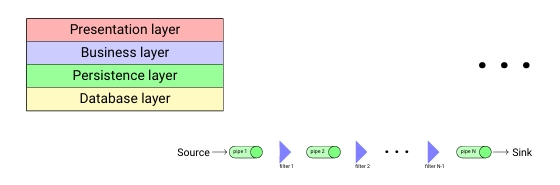
\includegraphics[width=1\textwidth]{Images/architectural style.jpeg}
\end{figure}
\subsubsection*{decisions concerning architecture}
\begin{itemize}
    \item \red{What} \blue{kind} of web framework shall be used?
    \item \red{What} are each layer's responsibilities?
    \item \red{Which} layers can communicate with each other?
    \item \red{What} exchange data formats must be used?
\end{itemize}
\subsubsection*{design principles}
\begin{itemize}
    \item NoSQL databases are the preferred storage option
    \item Immutable data structures are preferred
    \item Use asynchronous messaging between services when possible 
    \item Avoid usage of caching in clients
\end{itemize}
\subsection{Architecture and Design}
\subsubsection*{Demarcation line}
\begin{defBox}[title=Architects are responsible for ...]
    \begin{itemize}
        \item extracting the architecture characteristics from the requirement analysis
        \item choosing a set of styles for the software system
        \item creating the component structure (concise \& coherent parts of a system, above class level)
    \end{itemize}
\end{defBox}
\begin{figure}[h]
    \centering
    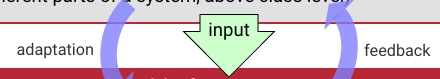
\includegraphics[width=0.5\textwidth]{Images/Demarcation line.jpeg}
\end{figure}
\begin{defBox}[title=Development team is responsible for ...]
    \begin{itemize}
        \item designing the class structure for each component (clss diagrams) (class structure must allow to meet the architecture characteristics)
        \item designing the user interface
        \item writing and testing the source code
    \end{itemize}
\end{defBox}
\begin{defBox}
    Modern architecture is \red{iterative} and incorporates feedback. Supporting \red{software evolution}.
\end{defBox}
\subsection{Architecture Characteristics}
\begin{defBox}[title=Architecture Characteristics]
    An \red{architecture characteristic} meets the following criteria:
    \begin{itemize}
        \item Specifies a \red{non-domain design consideration:} specifies operational and design criteria concerining \red{how to} implement a given requirement
        \item Influences a \red{structural design aspect}: requires the introduction of specific architectural elements (modules, components, ...), not merely \red{best practices} in design/coding
        \item Critical/important that application \red{performs as intended}: meets functional and non-functional requirements
    \end{itemize}
\end{defBox}
Whether a specific characteristic meets the above defined criteria may devend on the context of the software system
\begin{infoBox}
    \begin{enumerate}
        \item \fatsf{Definition eines Architedturmerkmals}\\
        Ein Architekturmerkmal erfüllt die folgenden Kriterien:
        \begin{enumerate}
            \item \fatsf{Es spezifiziert eine nicht-domänenspezifische Disignüberlegung:}
            \begin{itemize}
                \item \fatsf{Was bedeutet das?}
                \begin{itemize}
                    \item Das Merkmal konzentriert sich nicht auf die Geschäftslogik (z.B. das Buchen eines Termins), sondern auf \fatsf{wie} ein bestimmtes Verhalten oder eine Eigenschaft technisch umgesetzt wird.
                    \item Beispiel: Verfügbarkeit, Sicherheit oder Skalierbarkeit sind keine Domänenanforderungen, sondern technische Überlegungen.
                \end{itemize}
            \end{itemize}
            \item \fatsf{Es beeinflusst die strukturelle Gestaltung:}
            \begin{itemize}
                \item \fatsf{Was bedeutet das?}
                \begin{itemize}
                    \item Um das Merkmal zu erfüllen, müssen bestimmte \fatsf{architektonische Elemente} eingeführt werden, wie Module, Komponenten oder Services.
                    \item Es geht nicht nur um die Anwendung von Best Practices, sondern um Entscheidungen, die die gesamte Architektur beeinflussen.
                    \item Beispiel: Für Skalierbarkeit könnte man Microsevices einführen oder Lastenausgleichsmechanismen.
                \end{itemize}
            \end{itemize}
            \item \fatsf{Es ist kritisch/wichtig für die Funktionalität:}
            \begin{itemize}
                \item \fatsf{Was bedeutet das?}
                \begin{itemize}
                    \item Das System muss bestimmte funktionale und nicht-funktionale Anforderungen erfüllen. Ein Architekturmerkmal unterstützt die Umsetzung dieser Anforderungen.
                    \item Beispiel: Ein E-Commerce-System muss \fatsf{hohe Verfügbarkeit} sicherstellen, damit Nutzer jederzeit einkaufen können.
                \end{itemize}
            \end{itemize}
        \end{enumerate}
        \item \fatsf{Kontextabhängigkeit}
        ob ein bestimmtes Merkmal tatsätchlich als Architekturmerkmal gilt, hängt vom \fatsf{Kontext des Softwaresystem} ab:
        \begin{itemize}
            \item \fatsf{Beispiel:}
            \begin{itemize}
                \item Für ein Buchungssystem in einer Arztpraxis könnte \fatsf{Sicherheit} ein zentrales Architekturmerkmal sein.
                \item In einem internen Prototypensystem könnte Sicherheit weniger wichtig sein.
            \end{itemize}
        \end{itemize}
    \end{enumerate}
\end{infoBox}
\subsection{Architectureal Styles}
\subsubsection*{General}
\begin{defBox}[title=Architectural styles ...]
    \begin{itemize}
        \item help to specify the \red{fundamental structure} of a software system
        \item have impact on the appearance of \red{concrete software architectures}
        \item define a system's \red{global properties} such as:
        \begin{itemize}
            \item how distributed components cooperate and exchange data
            \item boundaries of subsystems
        \end{itemize}
    \end{itemize}
\end{defBox}
\begin{defBox}
    Software System are often composed of different architecture styles
\end{defBox}
\subsubsection{Examples}
\begin{defBox}[title=Examples of architectural styles]
    \blue{monolithic}
    \begin{itemize}
        \item \red{Layers}
        \item \red{Pipes and Filters}
        \item \red{Model-View-Controller}
    \end{itemize}
    \blue{distributed}
    \begin{itemize}
        \item \red{Service-Based}
        \item Broker
        \item Microservices
    \end{itemize}
\end{defBox}
\begin{defBox}[title=Choosing an architectural style]
    Choice of architectural style (almost) \red{always} comes with trade-offs.\\
    it is necessity to be aware of these, because additional measures might have to be taken to ensure that all architectuure characteristics are met.
\end{defBox}
\section{Monolithic Architectural Styles}
\begin{figure}[h]
    \centering
    \includegraphics[width=0.5\textwidth]{Images/Architectural Style: Layered.jpeg}
\end{figure}
\begin{infoBox}[title=Topologie und Schichten]
    Die Schichtenarchitektur organisiert Software in aufeinanderfolgende Ebenen (Layers), wobei jede Schicht spezifische Aufgaben übernimmt. Typische Schichten sind:
    \begin{itemize}
        \item \fatsf{Presentation Layer (Präsentationsschicht):} Interagiert mit Benutzern (z.B. UI oder API)
        \item \fatsf{Business Layer (Geschäftslogik):} Beinhaltet die Kernlogik des Systems und verarbeitet Daten gemäß den Anforderungen
        \item \fatsf{Persistence Layer (Datenpersistenz):} Verantwortlich für die Kommunikation mit der Datenbank
        \item \fatsf{Database Layer (Datenbankschicht):} Speicherort für die tatsächlichen Daten
    \end{itemize}
\end{infoBox}
\begin{defBox}[title=Topology]
    Number (and names) of layers not fixed. Some architectures ...
    \begin{itemize}
        \item unify business and persistence layer (business objects create SQL statements themselves)
        \item use additional layers (e.g., service) to enable reuse or restrict access
    \end{itemize}
\end{defBox}
\begin{infoBox}[title=Topologie: Anpassbarkeit der Schichten]
    \begin{itemize}
        \item \fatsf{Anzahl und Namen der Schichten:} Sind nicht fixiert, können je nach Anforderungen angepasst werden.
        \item \fatsf{Verschmelzung von Schichten:} Manche Architekturen kombinieren z.B. die \fatsf{Business}- und \fatsf{Persistence Layer}, indem Geschäftsobjekte direkt SQL-Statements erstellen.
        \item \fatsf{Zusätzliche Schichte:} Einige Architekturen fügen Schichten wie eine \fatsf{Service Layer} hinzu, um Wiederverwendung zu ermöglichen oder den Zugriff einzuschränken.
    \end{itemize}
\end{infoBox}
\begin{defBox}[title=Decisions concerning architecture]
    \begin{itemize}
        \item Definition of responsibilities for each layer
        \item Layer type (open or closed)
        \begin{itemize}
            \item Top-Down request must pass through closed layers, can skip open layers
            \item Open layers improve performance (less call chining), but reduce isolation
        \end{itemize}
    \end{itemize}
\end{defBox}
\begin{infoBox}[title=Entscheidungen bei der Architektur]
    \begin{itemize}
        \item \fatsf{Verantwortlichkeit jeder Schicht:} Jede Schicht hat klar definierte Aufgaben und sollte keine Verantwortung einer anderen Schicht übernehmen.
        \item \fatsf{Schichtentyp: Open vs. Closed Layers}
        \begin{itemize}
            \item \fatsf{Closed Layers (Geschlossene Schichten):} Alle Anfragen müssen die Schichten der Reihe nach durchlaufen.\\
            Vorteil: Klare Isolation der Verantwortlichkeit.\\
            Nachtiel: Kann die Leistung beeinträchtigen.
            \item \fatsf{Open Layers (Offene Schichten):} Anfragen können Schichten überspringen.\\
            Vorteil: Verbesserte Leistung (weniger Call-Chaining).\\
            Nachteil: Reduzierte Isolation und Wartbarkeit.
        \end{itemize}
    \end{itemize}
\end{infoBox}
\begin{defBox}[title=Trade Offs (selection)]
    + Simplicity and Cost
    + Reliability (medium)
    - Elasticity and scalability 
    - Performance: parallelization not inherently supported by architecture
    - Availability: usually long startup time / long mean time to recovery
\end{defBox}
\begin{infoBox}[title=Architectural Style: Layered (Trade-offs)]
    \begin{itemize}
        \item \fatsf{Vorteile:}
        \begin{itemize}
            \item \fatsf{Simplicity and Cost (Einfachheit und Kosten):} Einfach zu implementieren und günstig.
            \item \fatsf{Reliability (Zuverlässigkeit):} Mittlere Zuverlässigkeit durch klare Trennung der Schichten.
        \end{itemize}
        \item \fatsf{Nachteile:}
        \begin{itemize}
            \item \fatsf{Elasticity and Scalability (Elastizität und Skalierbarkeit):} Nicht optimiert für parallele Verarbeitung.
            \item \fatsf{Performance:} Kann bei vielen Schichten leiden.
            \item \fatsf{Availability (Verfügbarkeit:)} Lange Startzeiten und Ausfallwiederherstellung.
        \end{itemize}
    \end{itemize}
\end{infoBox}
\begin{defBox}[title=Summary]
    \begin{itemize}
        \item Technologically partitioned, \red{not} domain partitioned style
        \item Works well for \red{small} to \red{medium-size} applications
        \item Serves as \red{initial} architecture, can be changed later
        \item \red{Problematic:} Often not conscious decition, but result of Conway's law (Design reflicts organisational structure of the company)
    \end{itemize}
\end{defBox}
\begin{infoBox}[title=Zusammenfassung]
    \begin{itemize}
        \item \fatsf{Technologie Partitionierung:} \\
        Die Architektur ist nach technischen Aspekten (z.B. Datenbank, UI) gegliedert, nicht nach Domänenlogik.
        \item \fatsf{Eignung:}
        \begin{itemize}
            \item Gut geeignet für kleine bis mittelgroße Anwendungen.
            \item Häufig als Ausgangsarchitektur gewählt, später eventuell geändert.
        \end{itemize}
        \item \fatsf{Problem:}\\
        Oft nicht bewusst entschieden, sondern durch \fatsf{Conway's Law} bedingt: \enquote{Das Design eines Systems reflektiert die Organisationsstruktur des Unternehmens.}
    \end{itemize}
\end{infoBox}

\clearpage
\subsubsection*{Pipes and Filters}
\begin{figure}[h]
    \centering
    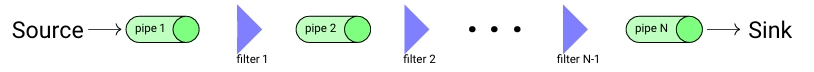
\includegraphics[width=1\textwidth]{Images/Pipes and Filters.jpeg}
\end{figure}
\begin{defBox}[title=Main topology]
    \begin{itemize}
        \item \red{Pipes}
        \begin{itemize}
            \item are \red{unidirectional, point-to-point channels} from a data source to a target
            \item allow any data format (i.e. not restricted by style); formats supporting smaller data chunks are preferred for better performance/throughput
        \end{itemize}
        \item \red{Filters} are
        \begin{itemize}
            \item \red{self-contained} and \red{independent} from other filters
            \item \red{stateless}, intuitively this means its operation does not depend on the past and should realize exactly \red{one} task 
        \end{itemize}
        \item Different kinds of \red{filters}
        \begin{itemize}
            \item \red{Producer:} Source of the data
            \item \red{Transformer:} (i) Receinves data from its input channel(s); (ii) performs operations on the data and (iii) forwards the result via its output channel
            \item \red{Consumer:} Sink of the data where it is output on the display, written to a file or database
        \end{itemize}
    \end{itemize}
\end{defBox}
\begin{infoBox}[title=Hauptkomponenten und ihre Funktionen]
    \begin{enumerate}
        \item \fatsf{Pipes (Kanäle):}
        \begin{itemize}
            \item \fatsf{Eigenschaften:}
            \begin{itemize}
                \item Datenflüsse sind \fatsf{unidirektional} (von einer Quelle zu einem Ziel)
                \item Sie verbinden die Filter miteinander
                \item Unterstützen beliebige Datenformate, bevorzugen jedoch Formate, die in \fatsf{kleinen Datenblöcken} verarbeitet werden können (verbessert die \fatsf{Performance und den Durchsatz})
            \end{itemize}
            \item \fatsf{Zweck:} Dienen als Transportmechanismus, um Daten zwischen den Filtern zu übertragen
        \end{itemize}
        \item \fatsf{Filters (Filter):}
        \begin{itemize}
            \item \fatsf{Eigenschaften:}
            \begin{itemize}
                \item Sind \fatsf{autonom} (arbeiten unabhängig von anderen Filtern)
                \item \fatsf{Zustandslos:} Sie speichern keine Informationen über vorherige Verarbeitungen. Jede Ausführung hängt vur von der aktuellen Eingabe ab
                \item \fatsf{Aufgabenorientiert:} Jeder Filter erfüllt genau \fatsf{eine Aufgabe}
            \end{itemize}
            \item \fatsf{Funktion:} Emjpfangen Daten über Eingabekanäle, verarbeiten sie, und senden die Ergebnisse über Ausgabekanäle weiter
        \end{itemize}
    \end{enumerate}
\end{infoBox}
\begin{infoBox}[title=Arten von Filtern]
    \begin{enumerate}
        \item \fatsf{Producer (Erzeuger):}
        \begin{itemize}
            \item Ursprung der Daten
            \item Beispiel: Ein Sensor, der Messwerte liefert
        \end{itemize}
        \item \fatsf{Transformer (Transformator):}
        \begin{itemize}
            \item \fatsf{Aufgaben:}
            \begin{enumerate}
                \item Daten über einen Eingabekanal empfangen
                \item Verarbeitungen durchführen (z.B. Transformation, Filterung, Berechnungen)
                \item Ergebnisse über den Ausgabekanal weiterleiten
            \end{enumerate}
            \item Beispiel: Ein Bildfilter, der Kontrastanpassungen durchführt.
        \end{itemize}
        \item \fatsf{Consumer (Verbraucher):}
        \begin{itemize}
            \item Endpunkt der Daten
            \item Beispiel: Eine Datenbank, in die Ergebnisse geschrieben werden, oder ein Anzeigesystem, das Ergebnisse darstellt
        \end{itemize}
    \end{enumerate}
\end{infoBox}
\begin{infoBox}[title=Zusammenfassung der Topologie]
    \begin{itemize}
        \item \fatsf{Pipes and Filters} folgt einem \fatsf{linearen oder verzweigten Ablauf:}
        \begin{itemize}
            \item Daten fließen von einem \fatsf{Producer} durch eine Reihe von \fatsf{Transformern} bis zu einem \fatsf{Consumer}
        \end{itemize}
        \item \fatsf{Vorteile:}
        \begin{itemize}
            \item \fatsf{Modularität:} Einfaches Hinzufügen oder Austauschen von Filtern
            \item \fatsf{Wiederverwendbarkeit:} Filter können unabhängig voneinander entwickelt werden
            \item \fatsf{Parallelität:} Datenströme können unabhängig verarbeitet werden, was die Leistung steigert.
        \end{itemize}
        \item \fatsf{Einschränkungen:}
        \begin{itemize}
            \item Kann ineffizient sein, wenn große Datenmengen verarbeitet werden oder Filter komplexe Aufgaben übernehmen
        \end{itemize}
    \end{itemize}
    Dieses Muster eignet sich besonders für Szenarien wie \fatsf{Datenverarbeitung in Echtzeit, Streaming} oder \fatsf{Bild-/Audioverarbeitung}
\end{infoBox}
\begin{figure}[h]
    \centering
    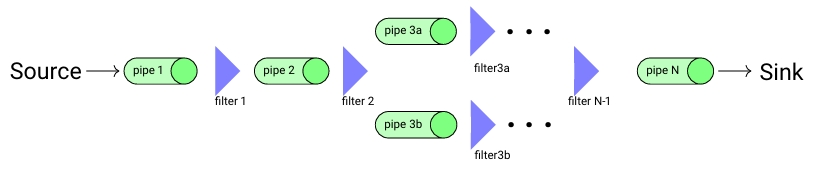
\includegraphics[width=1\textwidth]{Images/Variant topology.jpeg}
\end{figure}
\begin{defBox}[title=Variant topology (branching)]
    Additional kind of filter\\
    \red{Tester:} (i) Receives input; (ii) tests whether data satisfies certain conditions and (iii) redirects data according to outcome o tests to different output channels
\end{defBox}
\begin{infoBox}[title=Topologie]
    Die Topologie von Pipes and Filters sieht so aus:\\
    \fatsf{Quelle $\rightarrow$ Pipe 1 $\rightarrow$ Filter 1 $\rightarrow$ Pipe 2 $\rightarrow$ ... $\rightarrow$ Pipe N $\rightarrow$ Ziel}
    \begin{itemize}
        \item \fatsf{Quelle:} Der Startpunkt der Daten (z.B. eine Datei oder ein Eingabestream).
        \item \fatsf{Ziel:} Der Endpunkt, an dem die verarbeiteten Daten gespeichert, angezeigt oder weitergeleitet werden.
    \end{itemize}
\end{infoBox}
\begin{infoBox}[title=Beispielanwendung]
    \fatsf{Bildverarbeitung}
    \begin{itemize}
        \item \fatsf{Quelle:} Ein hochgeladenes Bild.
        \item \fatsf{Filter 1 (Weißabgleich):} Passt die Farben an.
        \item \fatsf{Filter 2 (Rauschunterdrückung):} Entfernt Bildrauschen.
        \item \fatsf{Filter 3 (JPEG-Kompression:)} Komprimiert das Bild, bevor es gespeichert wird.
        \item \fatsf{Ziel:} Speichert das bearbeitete Bild auf einer Festplatte.
    \end{itemize}
\end{infoBox}
\subsection{Architectural Style: Model-View-Controller (MVC)}
\subsubsection*{Main Topology}
\begin{defBox}
    Fundamental struchtural organization for interactive software systems
\end{defBox}
\begin{figure}[h]
    \centering
    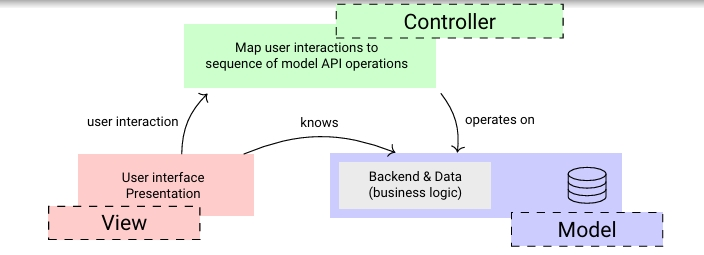
\includegraphics[width=1\textwidth]{Images/Main Topology.jpeg}
\end{figure}
\begin{defBox}[title=Main Topology]
    \begin{itemize}
        \item Separates system in three modules: Model-View-Controller
        \begin{itemize}
            \item \red{Model:} business logic and data storage independent of
            \begin{itemize}
                \item input behavior
                \item output representation
            \end{itemize}
            \item \red{View:} presentation of (parts of) the model data to the user
            \begin{itemize}
                \item data obtained from model
                \item frequently more than one (different kind of) view
            \end{itemize}
            \item \red{Controller:} translates user interactions to operations on the model
            \begin{itemize}
                \item each view is associated to a controller
                \item all interactions via controller
            \end{itemize}
        \end{itemize}
        \item Controller and View are \red{directly coupled with the Model}
        \item Model is \red{not directly coupled with the Controller or the View}
    \end{itemize}
\end{defBox}

\subsubsection*{Change Propagation}
\begin{figure}[h]
    \centering
    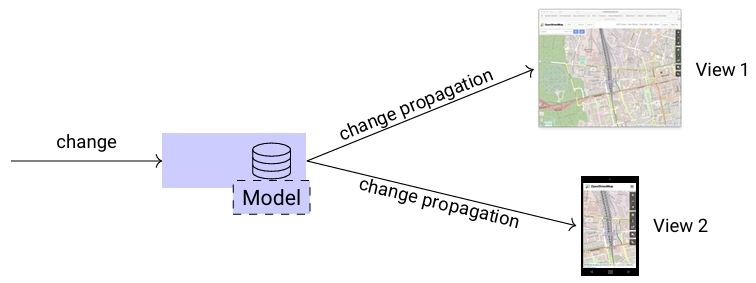
\includegraphics[width=1\textwidth]{Images/Change Propagation.jpeg}
\end{figure}
\begin{defBox}[title=Change Propagation]
    A \red{change propagation mechanism} ensures consistency between the user interface and the model (Often implemented using the Observer/Publisher-Subscriber pattern; see later lacture)
\end{defBox}
\begin{defBox}[title=Basic Idea]
    \begin{itemize}
        \item Views \red{register} themselves at a model (Controllers, whose behavior depends on the model state, register themselves also at the model)
        \item Model \red{notifies} registered view objects upon change
    \end{itemize}
\end{defBox}

\clearpage
\subsubsection*{CaSh-Static structure}
\begin{figure}[h]
    \centering
    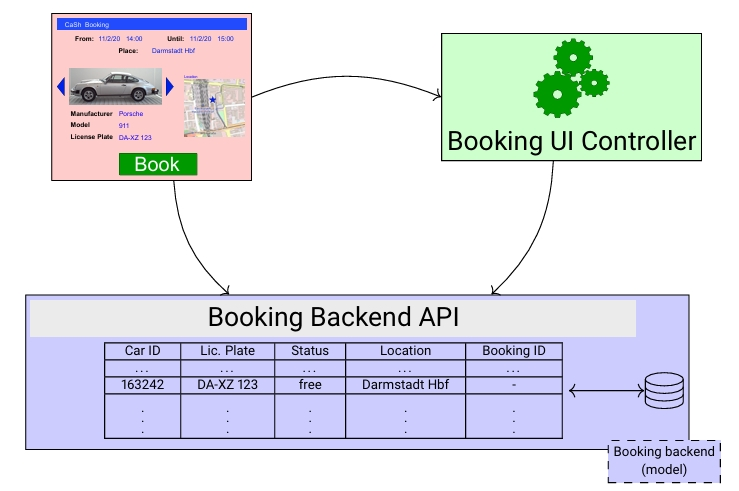
\includegraphics[width=0.65\textwidth]{Images/CaSh-Static structure.jpeg}
\end{figure}

\subsubsection*{CaSh - Dynamic}
\begin{figure}[h]
    \centering
    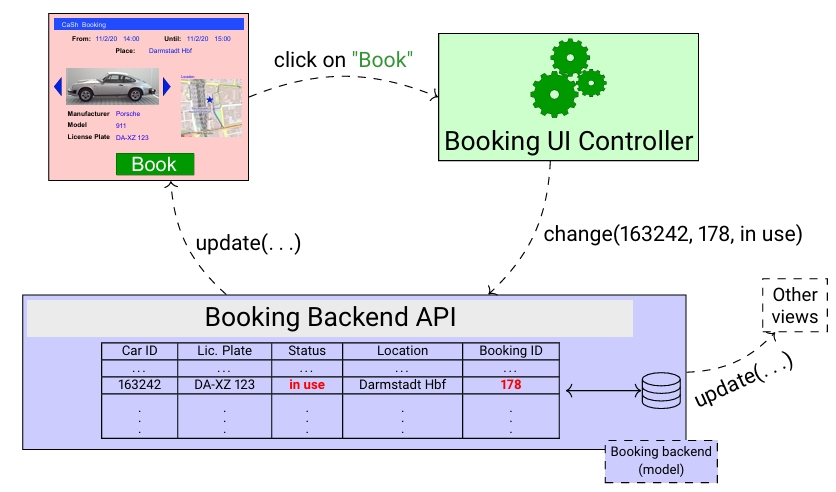
\includegraphics[width=0.75\textwidth]{Images/CaSh-Dynamic.jpeg}
\end{figure}

\subsubsection*{Applicability and Trade-Offs}
\begin{defBox}[title=When to use MVC]
    Applicaton is interactive and:
    \begin{itemize}
        \item the model data should be presented in different ways
        \item number and kind of views are not fixed (and/or unknown)
        \item display and application behavior must reflect data changes immediately
        \item changing and porting the UI should not affect the application's core
    \end{itemize}
\end{defBox}
\begin{defBox}[title=Trade-Offs]
    \begin{enumerate}
        \item Update proliferation, \red{but} not all views are interested in all changes
        \item Increase in complexity ue to separate view and controller components without gaining much flexibility
        \item High dependency (coupling)betwenn view and controller
    \end{enumerate}
\end{defBox}
\begin{infoBox}[title=Wann sollte MVC verwendet werden?]
    \begin{enumerate}
        \item \fatsf{Interaktive Anwendungen:}
        \begin{itemize}
            \item Wenn Benutzereingaben Änderungen an Daten erfordern und diese sofort in der Oberfläche (UI) sichtbar sein müssen
        \end{itemize}
        \item \fatsf{Mehrere Darstellungen:}
        \begin{itemize}
            \item Wenn dieselben Daten (\fatsf{Model}) in \fatsf{verschiedenen Ansichten oder Formaten} dargestellt werden sollen (z.B. als Liste oder Diagramm)
        \end{itemize}
        \item \fatsf{Dynamische Ansichten:}
        \begin{itemize}
            \item Wenn die \fatsf{Anzahl und Art der Ansichten nicht festgelegt} oder im Voraus bekannt sind und sich im Laufe der Zeit ändern können
        \end{itemize}
        \item \fatsf{Trennung von Logik und UI:}
        \begin{itemize}
            \item Wenn das Ändern oder Portieren der \fatsf{Benutzeroberfläche (UI)} unabhängig vom Kern der Anwendung erfolgen soll
        \end{itemize}
    \end{enumerate}
\end{infoBox}
\begin{infoBox}[title=Trade-offs von MVC]
    \begin{enumerate}
        \item \fatsf{Update-Welle:}
        \begin{itemize}
            \item \fatsf{Problem:} Änderungen am Model benachrichtigen \fatsf{alle Views}, selbst wenn nicht alle die Änderung benötigen
            \item \fatsf{Auswirkung:} Dies kann zu unnötigem Aufwand und Leistungseinbußen führen
        \end{itemize}
        \item \fatsf{Erhöhte Komplexität:}
        \begin{itemize}
            \item \fatsf{Problem:} Die strikte Trennung zwichen Model, View und Controller führt zu mehr \fatsf{Komponenten}, was die Entwicklung komplizierter macht
            \item \fatsf{Auswirkung:} Wenn Flexibilität nicht entscheidend ist, kann die zusätzliche Komplexität unnötig sein
        \end{itemize}
        \item \fatsf{Abhängigkeit zwischen View und Controller:}
        \begin{itemize}
            \item \fatsf{Problem:} View und Controller sind oft \fatsf{stark gekoppelt}, was die Wiederverwendbarkeit einschränkt und Abhängigkeiten erhöht
            \item \fatsf{Auswirkung:} Änderungen an einer Komponente können die andere beeinträchtigen, was die Modularität verringert
        \end{itemize}
    \end{enumerate}
\end{infoBox}

\clearpage
\section{Distributed Architectural Styles}
\subsection{Architectural Style: Service-Based}
\subsubsection*{Main Topology}
\begin{figure}[h]
    \centering
    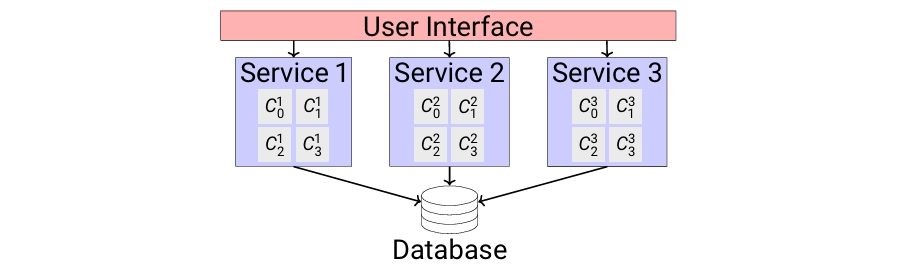
\includegraphics[width=1\textwidth]{Images/Service-Based.jpeg}
\end{figure}
\begin{defBox}[title=Main Topology]
    \begin{itemize}
        \item One monolithic user interface for all services
        \item Each service i is composed of different components $C^{i}_{j}$
        \item Services share a common database
    \end{itemize}
\end{defBox}
\begin{infoBox}[title=Haupttopologie des Service-Based-Stils]
    \begin{enumerate}
        \item \fatsf{Monolithische Benutzeroberfläche (UI):}
        \begin{itemize}
            \item In dieser Architektur gibt es \fatsf{ein zentrales Benutzerinterface}, das alle Dienste bedient. Das bedeutet, dass der Benutzer über eine einzige Oberfläche mit allen Services interagiert
            \item Diese Oberfläche ist dafür verantwortlich, Anfragen an die verschiedenen Services zu stellen und die Ergebnisse entsprechend anzuzeigen
        \end{itemize}
        \item \fatsf{Services und ihre Komponenten:}
        \begin{itemize}
            \item Jeder \fatsf{Service} (z.B. für eine bestimmte Funktion wie Benutzerverwaltung oder Zahlungsabwicklung) besteht aus mehreren \fatsf{Komponenten}
            \item Jede Komponente innerhalb eines Services ist für eine bestimmte Aufgabe zuständig, aber alle zusammen ermöglichen sie die vollständige Funktionalität des Services
            \item Die Komponenten innerhalb eines Services arbeiten eng zusammen, um eine konsistente Dienstleistung bereitzustellen
        \end{itemize}
        \item \fatsf{Gemeinsame Datenbank:}
        \begin{itemize}
            \item Alle \fatsf{Services} in diesem Modell teilen sich eine \fatsf{gemeinsame Datenbank}
            \item Das bedeutet, dass alle Services auf dieselben Daten zugreifen und diese verwalten. Es gibt keine separate Datenbank für jeden Service
            \item Diese Struktur kann dazu führen, dass es eine \fatsf{engere Kopplung} zwischen den Services und der Datenbank gibt, was manchmal die Skalierbarkeit und Flexibilität einschränken kann, jedoch einfacher für klienere bis mittlere Systeme ist
        \end{itemize}
    \end{enumerate}
\end{infoBox}

\subsubsection*{Topology Variants}
\begin{defBox}[title=Non-monolithic user interfaces]
    \begin{itemize}
        \item Domain-based user interface
        \item Service-based user interface (one UI per service; not shown)
    \end{itemize}
\end{defBox}
\begin{infoBox}[title=Nicht-monolitische Benutzeroberflächen]
    \begin{enumerate}
        \item \fatsf{Domänenbasierte Benutzeroberfläche:}
        \begin{itemize}
            \item Bei diesem Ansatz wird die Benutzeroberfläche (UI) basierend auf den \fatsf{Domänen} (also den Hauptbereichen der Anwendung, wie z.B. Kundenmanagement, Bestllverwaltung, etc.) strukturiert
            \item Jede Domäne erhält eine eigene Benutzeroberfläche, die spezifische Funktionen und Interaktionen für diese Domäne bereitstellt
            \item Die Vorteile liegen in der besseren \fatsf{Trennung der Anliegen} und einer klareren Struktur der UI, da jede Domäne ihr eigenes UI hat
        \end{itemize}
        \item \fatsf{Service-basierte Benutzeroberfläche:}
        \begin{itemize}
            \item In diesem Fall gibt es für \fatsf{jeden Service} eine separate Benutzeroberfläche. Jeder Service hat sein eigenes I, das auf die Funktionalität dieses Services fokussiert ist
            \item Diese Architektur ermöglicht eine \fatsf{sehr hohe Flexibilität} und Modularität, da jeder Service unabhängig von den anderen seine eigene UI-Logik hat
        \end{itemize}
        \item \fatsf{Vorteil:} Veränderungen oder Erweiterungen eines Services können vorgenommen werden, ohne die UI anderer Services zu beeinträchtigen
        \item \fatsf{Nachteil:} Es kann zu einer erhöhten Komplexität führen, da mehrere UIs verwaltet werden müssen
    \end{enumerate}
\end{infoBox}
\begin{figure}[h]
    \centering
    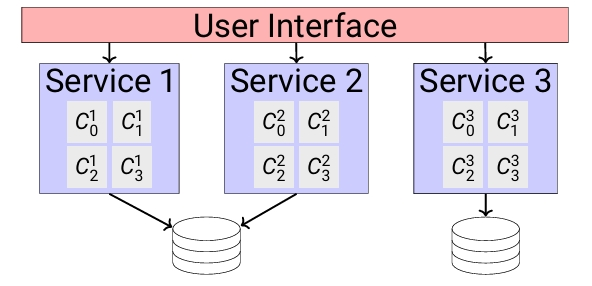
\includegraphics[width=0.9\textwidth]{Images/Database Location.jpeg}
\end{figure}
\begin{defBox}[title=Database Location]
    \begin{itemize}
        \item Service-local databases
        \begin{itemize}
            \item Data owned by one service (opne service type)\\
            all queries and changes must use service API
            \item Structure supports data consistency and easier scalability
        \end{itemize}
        \item Miced configuration of shared and service-local databases (shown)
        \begin{itemize}
            \item Shared databases (esp. shared schemas) require coordination
            \item Data ownership must be clearly defined \\
            Target: One service has write permissions, multiple may read
        \end{itemize}
    \end{itemize}
\end{defBox}
\begin{infoBox}[title=Datenbankkonfigurationen]
    \begin{enumerate}
        \item \fatsf{Service-lokale Datenbanken:}
        \begin{itemize}
            \item In diesem Modell besitzt jeder \fatsf{Service sein eigene Datenbank}. Das bedeutet, dass jeder Service für seine Daten verantwortlich ist und sämtliche \fatsf{Abfragen und Änderungen} nur über die API des jeweiligen Services durchgeführt werden
            \item \fatsf{Vorteil:} Durch die Trennung der Datenbank je Service wird eine klare \fatsf{Datenkonsistenz} gewährleistet. Zudem ist diese Struktur sehr \fatsf{skalierbar,} da Services unabhängig voneinander skaliert werden können, ohne die Datenbank jedes anderen Services zu beeinflussen
            \item \fatsf{Nachteil:} Es könnte eine größere \fatsf{Datenwiederholung} geben, wenn mehrere Services ähnliche Daten benötigen
        \end{itemize}
        \item \fatsf{Gemischte Konfiguration von geteilten und Service-lokalten Datenbanken:}
        \begin{itemize}
            \item In dieser Konfiguration gibt es sowohl \fatsf{geteilte Datenbanken} (die von mehreren Services genutzt werden) als auch \fatsf{lokale Datenbanken} für bestimmte Services
            \item \fatsf{Vorteil:} Diese Struktur bietet eine gewisse \fatsf{Flexibilität}, da mehrere Services auf dieselben Daten zugreifen können. Sie erfordert jedoch eine sorgfältige \fatsf{Koordination} bei der Verwaltung der gemeinsamen Daten.
            \item \fatsf{Herausforderung:} Der \fatsf{Datenbesitz} muss klar definiert werden, um sicherzustellen, dass nur ein Service \fatsf{Schreibrechte} auf die Daten hat, während andere Services nur \fatsf{Lesezugriff} erhalten. Diese klare Definition ist notwendig, um \fatsf{Datenkonsistenz} und Konflikte zu vermeiden
            \item \fatsf{Nachteil:} Besonders bei \fatsf{gemeinsam genutzten Datenbanken (z.B. bei geteilten Schemata)} ist eine strenge \fatsf{Koordination und Synchronisation} erforderlich, um sicherzustellen, dass keine Dateninkonsistenzen oder Konflikte zwischen den Services entstehen
        \end{itemize}
    \end{enumerate}
\end{infoBox}
\subsubsection*{CaSh}
\begin{figure}[h]
    \centering
    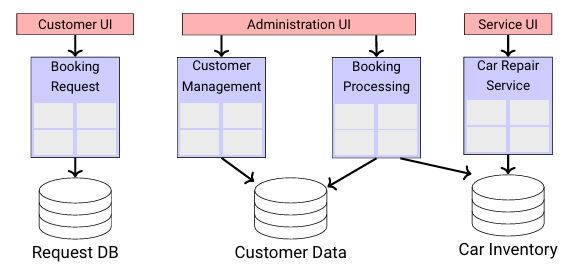
\includegraphics[width=0.9\textwidth]{Images/A service-based architecture for CaSh.jpeg}
\end{figure}
\begin{defBox}[title=A service-based architecture for CaSh]
    \begin{itemize}
        \item Customer UI uses \red{Booking Request} service to generate a booking request
        \item Booking request sent to \red{Booking Processing} service
        \item Service accessible for customer has no direct access to company databases (architecture supports security aspects)
    \end{itemize}
\end{defBox}
\subsubsection*{CaSh - Service Structure}
\begin{figure}[h]
    \centering
    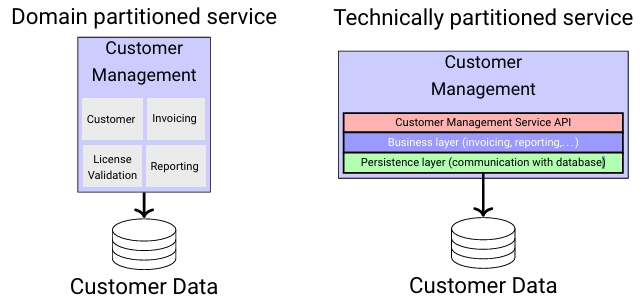
\includegraphics[width=1\textwidth]{Images/CaSh - Service Structure.jpeg}
\end{figure}
\begin{defBox}[title=CaSh: Two alternatice service architectures]
    \begin{itemize}
        \item \red{Domain partitioned} service: components realize domain specific tasks
        \item \red{Technically partitioned} service: components organized as layered structure
    \end{itemize}
\end{defBox}
\begin{infoBox}
    \begin{itemize}
        \item \fatsf{Domain-partitionierte Architektur} ist ideal für Systeme, bei denen die \fatsf{geschäftlichen Domänen} voneinander getrennt sind und klare Verantwortlichkeiten bestehen. Es eignet sich gut für \fatsf{business-orientierte Anwendungen}
        \item \fatsf{Technisch partitionierte Architektur} (Schichtenarchitektur) ist sinnvoll für Anwendungen, bei denen die \fatsf{technischen Aspekte} wie Datenhaltung, Geschäftslogik und Benutzeroberfläche klar voneinander getrennt werden müssen. Es eignet sich gut für \fatsf{technologisch komplexe Systeme}
    \end{itemize}
\end{infoBox}
\clearpage
\section{Wrapping Up}
\subsection{Choosing an Architectural Style}
\subsubsection*{Influences}
\begin{figure}[h]
    \centering
    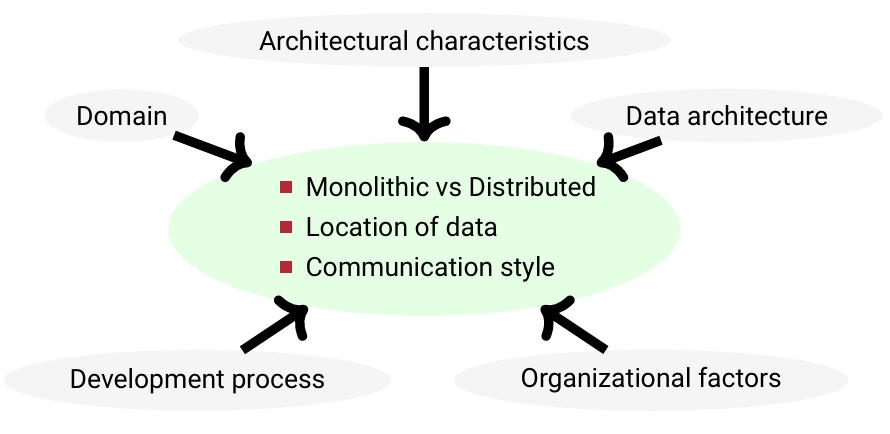
\includegraphics[width=0.9\textwidth]{Images/Choosing an Architectural Style.jpeg}
\end{figure}

\subsection{Decisions Concerning Architecture}
\subsubsection*{Soft Skills}
\begin{defBox}[title=Fear of the wrong decision]
    Decision is avoided/deferred out of fear to make the wrong choice\\
    Possible solution:
    \begin{itemize}
        \item make decistion at \enquote{last \red{responsible} moment}\\
        at a time early enough so that the missing decision does not cause delay to other work
        \item stay clase to development team to be able to react to problems
    \end{itemize}
\end{defBox}
\begin{defBox}[title=Never ending discussions]
    Decision discussed over and over again because reason \red{why} is not known
\end{defBox}
\begin{defBox}[title=Architecture not implemented]
    Architecture not implemented by developers because decisions are not known
\end{defBox}
Both problem are essentially about documentation and communication
\begin{itemize}
    \item Document decisions at a well-known and suitable place
    \begin{itemize}
        \item Formal document
        \item Better: wiki with attached issue tracker used by development team
    \end{itemize}
    \item Choose appropriate media to cummunicate (changes to) decisions
    \item Keep messages concise, refer to wiki/issue tracker/document for details
\end{itemize}
\begin{infoBox}[title=Entscheidungen zur Architektur: Herausforderungen und Lösungen]
    Architekturentscheidungen sind ein zentraler Bestandteil der Softwareentwicklung. Dabei können jedoch typische Herausforderungen auftreten, die durch gezielte Maßnahmen adressiert werden sollten:
    \begin{enumerate}
        \item \fatsf{Angst vor falschen Entscheidungen}
        \begin{itemize}
            \item \fatsf{Problem:} Entscheidungen werden vermieden oder verzögert, aus Angst, eine falsche Wahl zu treffen
            \item \fatsf{Konsequenzen:} Verzögerungen in der Entwicklung, Unsicherheit im Team, mangelnde Fortschritte
            \item \fatsf{Lösungen:}
            \begin{itemize}
                \item \fatsf{Entscheidung zum \enquote{last responsible moment} treffen:}
                \begin{itemize}
                    \item Entscheidungen so spät wie möglich, aber rechtzeitig treffen, damit keine Verzögerungen im Projekt entstehen
                \end{itemize}
                \item \fatsf{Nähe zum Entwicklungsteam:}
                \begin{itemize}
                    \item Enger Kontakt ermöglicht, frühzeitig auf Probleme zu reagieren und fundierte Entscheidungen zu treffen
                \end{itemize}
            \end{itemize}
        \end{itemize}
        \item \fatsf{Endlose Diskussionen}
        \begin{itemize}
            \item \fatsf{Problem:} Entscheidungen werden wiederholt diskutiert, da die Gründe für die Entscheidung nicht klar sind
            \item \fatsf{Konsequenzen:} Zeitverlust, ineffizientes Arbeiten, Verzögerungen bei der Umsetzung
            \item \fatsf{Lösung:}
            \begin{itemize}
                \item \fatsf{Dokumentation:}
                \begin{itemize}
                    \item Die Gründe und Rahmenbedingungen von Entscheidungen sollten an einer \fatsf{bekannten und zugänglichen Stelle} dokumentiert werden
                    \item Beispiele: formale Dokumente, besser jedoch ein Wiki mit angebundenem \fatsf{Issue Tracker}, das vom Entwicklungsteam genutzt wird
                \end{itemize}
            \end{itemize}
        \end{itemize}
        \item \fatsf{Architektur wird nicht umgesetzt}
        \begin{itemize}
            \item \fatsf{Problem:} Entwickler setzen die Architektur nicht um, weil sie die Entscheidungen nicht kennen oder verstehen
            \item \fatsf{Konsequenzen:} Die Architektur bleibt Theorie, mangelnde Kohärenz im Systemdesign
            \item \fatsf{Lösung:}
            \begin{itemize}
                \item \fatsf{Kommunikation verbessern:}
                \begin{itemize}
                    \item Entscheidungen und Änderungen über \fatsf{geeignete Medien} kommunizieren
                    \item \fatsf{Nachrichtensystematik:}
                    \begin{itemize}
                        \item Kurze, prägnante Nachrichten
                        \item Für Details auf die dokumentierten Entscheidungen im Wiki oder Issue Tracker verweisen
                    \end{itemize}
                \end{itemize}
            \end{itemize}
        \end{itemize}
    \end{enumerate}
\end{infoBox}
\clearpage
\section{Design Principles 1}
\section{Part I: Dimensions of Software Quality}
\subsection{Software Quality}
\begin{defBox}[title=How to assure software quality? The big picture]
    Define a \red{quality assurance (QA) plan} (\enquote{\blue{Plan zur Qualitätssicherung}}) (must be integrated into the software development process)
    \begin{itemize}
        \item Constatly \red{assess} design \red{quality} (quantitative, qualitative)
        \item Be proficient in applying time-tested \red{design principles}
        \item Use tools and \red{design techniques} that help to achieve quality 
        \item Use \red{design patterns} to learn from and reuse proven slutions to recurring problems
        \item Systematically \red{verify} correctness \& performance of design 
        \item\red{Validate} fulfillment of requirements
    \end{itemize}
\end{defBox}
\begin{infoBox}
    \begin{enumerate}
        \item \fatsf{QA-Plan definieren}
        \begin{itemize}
            \item A \fatsf{Qualitätssicherungsplan (QA) plan} ist unverzichtbar und muss in den Softwareentwicklungsprozess integriert werden. Der Plan beschreibt Aktivitäten , Zeitplänne, Werkzeuge und Rollen, um die Qulität während des gesamten Entwicklungsprozesses sicherzustellen.
        \end{itemize}
        \item \fatsf{Designqualität kontinuierlich bewerten}
        \begin{itemize}
            \item Das Design sollte regelmäßíg anhand \fatsf{quantitativer} (z.B. Metriken) und \fatsf{qualitativer} (z.B. Expertenbewertungen) Methoden überprüft werden, um Probleme frühzeitig zu erkennen und zu beheben.
        \end{itemize}
        \item \fatsf{Bewährte Designprinzipien anwenden}
        \begin{itemize}
            \item Durch die Einhaltung bewährter \fatsf{Designprinzipien} (z.B. SOLID, DRY, KISS) wird sichergestellt, dass die Software robust und wartbar bleibt.
        \end{itemize}
        \item \fatsf{Nutzung von Werkzeugen und Techniken}
        \begin{itemize}
            \item Verwenden Sie Tools (z.B. statische Code-Analyse, CI/CD-Pipelines) und Techniken (z.B. testgetriebene Entwicklung, Paarprogrammierung), die den Entwicklungsprozess effizienter und qualitativ hochwertiger machen.
        \end{itemize}
        \item \fatsf{Design Patterns einsetzen}
        \begin{itemize}
            \item \fatsf{Design Patterns} bieten wiederverwendbare, bewährte Lösungen für häufig auftretende Probleme und minimieren Fehlerquellen.
        \end{itemize}
        \item \fatsf{Korrektheit und Leistung überprüfen}
        \begin{itemize}
            \item Systematische Überprüfungsmethoden wie Tests (Unit-, Integrations-, und Systemtests) oder Performance-Analysen helfen sicherzustellen, dass das Design die Anforderungen erfüllt.
        \end{itemize}
        \item \fatsf{Erfüllung der Anforderungen validieren}
        \begin{itemize}
            \item Die entwickelte Software sollte fortlaufend mit den definierten Anforderungen abgeglichen werden, um sicherzustellen, dass sie die vorgesehenen Funktionalitäten und Leistungsziele erreicht.
        \end{itemize}
    \end{enumerate}
\end{infoBox}

\subsection{Internal and External Quality Factors}
\begin{defBox}[title=What is good software?]
    \red{Internal quality factors} - Perceivable only by computer professionals
    \begin{itemize}
        \item \blue{White box} view of a software system
    \end{itemize}
    \red{External quality factors} - Perceived by the customer \/ user
    \begin{itemize}
        \item \blue{Black box} view of a softare system
        \item Depend on internal quality factors
    \end{itemize}
\end{defBox}
\begin{infoBox}[title=Was ist gute Software?]
    Gute Software zeichnet sich durch interne und externe Qualitätsfaktoren aus, die verschiedene Perspektiven auf die Qualität eines Softwaresystems bieten:
\end{infoBox}
\begin{infoBox}[title=Interne Qualitätsfaktoren]
    \begin{itemize}
        \item \fatsf{Definition:} Aspekte, die nur von Computerprofis (Entwicklern, Architekten) whargenommen werden können.
        \item \fatsf{Whitebox-Perspektie:} Betrachtung des inneren Aufbaus der Software, z.B. des Codes und der Architektur
        \item \fatsf{Beispiele:}
        \begin{itemize}
            \item \fatsf{Wartbarkeit:} Wie leicht kann der Code verändert oder erweitert werden?
            \item \fatsf{Lesbarkeit:} Ist der Code verständlich und klar strukturiert?
            \item \fatsf{Modularität:} Ist die Software in sinnvolle Einheiten zerlegt?
            \item \fatsf{Fehlerfreiheit:} Sind interne Fehlerquellen minimiert?
        \end{itemize}
    \end{itemize}
\end{infoBox}
\begin{infoBox}[title=Externe Qualitätsfaktoren]
    \begin{itemize}
        \item \fatsf{Definition:} Eigenschaften, die direkt von Kunden oder Endnutzern whargenommen werden.
        \item \fatsf{Blackbox-Perspektive:} Fokus auf die Funktionalität und Leistung der Software, ohne die interne Struktur zu kennen.
        \item \fatsf{Beispiele:}
        \begin{itemize}
            \item \fatsf{Benutzerfreundlichkeit:} Ist die Software intuitiv und leicht zu bedienen?
            \item \fatsf{Zuverlässigkeit:} Funktioniert die Software stabil und fehlerfrei?
            \item \fatsf{Leistung (Performance):} Läuft die Software effizient und schnell?
            \item \fatsf{Sicherheit:} Schützt die Software vor unberechtigtem Zugriff und Datenverlust?
        \end{itemize}
    \end{itemize}
\end{infoBox}
\subsection{Software Quality: Internal Factors}
\begin{defBox}[title=Some important internal quality factors]
    \begin{itemize}
        \item \red{Modularity}
        \item \red{Comprehensibility} (\enquote{\blue{Verständlichkeit}}), not overly complex
        \item \red{Cohesion:} clear responsibilities
        \item \red{Concision} (\enquote{\blue{Prägnanz}}): little code duplication, clear code
        \item \red{Correctness}
    \end{itemize}
\end{defBox}
\begin{defBox}
    We will talk about how to judge and how to ensure these quality factors
\end{defBox}
\subsection{Software Quality: External Factors}
\begin{defBox}[title=External quality facotrs\, perceived by Costomer or User]
    \begin{itemize}
        \item \fatsf{Validity:} The ability of software to perform as defined in its requirements
        \begin{itemize}
            \item \red{Precise requirements} definition is needed
            \item Validity depends on correct \red{design}
            \item Validity is often \red{conditional} to correctness of lower layers: Compiler, OS, vertual machine, hardware, etc. 
        \end{itemize}
        \item \fatsf{Robustness:} The ability of software systems to react appropriately to abnormal conditions \blue{outside of the operational specification}
        \item \fatsf{Extensibility:} Ease of adapting software products to \blue{extended} requirements
        \begin{itemize}
            \item \red{Architecture:} Can the architecture be easily adapted?
            \item \red{Modularity:} Loose coupling (to be defined precisely) makes changes easy
        \end{itemize}
        \item \fatsf{Reusability:} The ability of software elements to serve for the construction of further applications
        \item \fatsf{Compatibility / Interoperability:} Ease of combining software elements with other applications:
        \begin{itemize}
            \item Compatibility to \red{standards}, protocols
            \item \red{Backwards} compatible (to itself)
            \item \red{Interoperable} with other (legacy) applications
        \end{itemize}
        \item \fatsf{Portability:} Ease of transferring software products to other hardware and software environments
        \item \fatsf{Efficiency:} The ability of a software system to use hardware resources \red{economically}
        \begin{itemize}
            \item CPU time/load, internal/external memory usage, power, bandwidth, etc
            \item Often depends on choice of \red{algorithm} (different course)
            \item \red{Inverst in common case:} Efficiency often has to be traded off
        \end{itemize}
        \item \fatsf{Usability:} How easily people with different backgrounds and qualifications can \red{learn} to use software and \red{apply} it to solve problems
        \item \fatsf{Functionality (meets expectations) (Features):} Extent of possible usage modes provided by a system
        \begin{itemize}
            \item Avoid \enquote{featurism}: ensure consistency of new features with existing ones
        \end{itemize}
    \end{itemize}
\end{defBox}
\subsection{Main Attributes of \enquote{Good} Software}
\begin{itemize}
    \item \red{Maintainability:} Constructed in such a way that it may \red{evolve} to meet changing requirements of customers
    \item \red{Efficiency:} Does \red{not wast} system resources: Processing time, memory utilisation, energy, bandwidth, etc.
    \item \red{Usability:} Responsiveness, must be usable by the intended users
    \item \red{Dependability:} \enquote{\blue{Verlässlichkeit}} Does not cause physical or economic damage in the event of system failure\\
    Sub-properties: repairability, survivability, fault tolerance Belongs to \red{systemengineering} rather than SE
\end{itemize}

\section{Quantitative Measures of Software Quality}
\subsection{From Software Quality to Code Quality}
\begin{defBox}[title=How to measure software quality?]
    \red{There is no generally accepted measure of software quality!}
    \begin{itemize}
        \item There are \red{many} qualities in software (as seen)\\
        Some of these are at odds to each other (for example, usability - security)
        \item \blue{What we can do:}\\
        Define \red{heuristics} that \red{indicate} the quality of \red{code}
        \item These heuristics are called \red{software metrics} (better: \red{code metrics})
    \end{itemize}
\end{defBox}
\begin{infoBox}[title=Ansätze zur Bewertung der Softwarequalität]
    \fatsf{Heuristiken und Metriken}
    \begin{itemize}
        \item \fatsf{Definition:} Heuristiken sind Regeln oder Ansätze, die helfen, die Qualität des Codes zu bewerten. Diese werden in der Praxis durch \fatsf{Softwaremetriken} (besser: \fatsf{Codemetriken}) ergänzt.
        \item \fatsf{Ziel:} Hinweise auf schlechte Codequalität oder Designprobleme geben.
    \end{itemize}
\end{infoBox}
\begin{defBox}[title=Software Metrics Pro]
    \begin{itemize}
        \item Can be computed \red{mechanically}
        \item May indicate \red{bad design}
    \end{itemize}
\end{defBox}
\begin{infoBox}[title=Vorteile von Softwaremetriken]
    \begin{enumerate}
        \item \fatsf{Mechanische Berechnung}
        \begin{itemize}
            \item Können automatisiert mit Werkzeugen wie SonarQube, Checkstyle etc. berechnet werden.
            \item Beispiele: \fatsf{Zeilenanzahl, Komplexität (Cyclomatic Complexity), Anzahl der Abhängigkeiten.}
            \item \fatsf{Frühzeitige Hinweise}
            \begin{itemize}
                \item Identifizieren potenziell problematische Bereiche im Code, z.B. übermäßig komplexe Module oder mangelnde Modularität.
            \end{itemize}
        \end{itemize}
    \end{enumerate}
\end{infoBox}
\begin{defBox}[title=Software Metrics Contra]
    \begin{itemize}
        \item No notion of \red{semantics} of code
        \item False sense of \red{correctness}
    \end{itemize}
\end{defBox}
\begin{infoBox}[tile=Nachteile von Softwaremetriken]
    \begin{enumerate}
        \item \fatsf{Keine Berücksichtigung der Semantik}
        \begin{itemize}
            \item Softwaremetriken bewerten nur \fatsf{syntaktische Aspekte}, nicht die Bedeutung oder Funktionalität des Codes.
            \item Beispiel: Ein \enquote{gut strukturierter} Code könnte immer noch fehlerhaft sein.
        \end{itemize}
        \item \fatsf{Gefühl der falschen Sicherheit}
        \begin{itemize}
            \item Metriken können ein \fatsf{falsches Gefühl der Korrektheit} erzeugen, wenn sie isoliert betrachtet werden.
            \item Guter \enquote{metrischer Code} ist nicht automatisch fehlerfrei oder für alle Zwecke geeignet.
        \end{itemize}
    \end{enumerate}
\end{infoBox}
\subsection{Code Metrics to Identify Anomalies}
\begin{defBox}[title=Some software metrics]
    \begin{itemize}
        \item \red{Fan in/fan out:} \\
        \blue{Fan-in} of method m = \# of methods \blue{calling} m\\
        \blue{Fan-out} of method m = \# of method \blue{called by} m
        \item \red{Length of code:} Length of source code (indicator of complexity)
        \item \red{Cyclomatic complexity:} Independent paths through code (in \blue{control-flow graph})
        \item \red{Depth of conditional nesting:} Deep nesting hard to understand: Increased test effort
        \item \red{Weighted methods per class:} Method weight depends on size/comlexity, summed up per class
        \item \red{Depth of inheritance tree:} Deep inheritance tree: Classes depend on many design constraints
    \end{itemize}
\end{defBox}
\subsection{Control-Flow Graph (CFG)}
\red{Control-flow graph} (CFG) represents all execution sequences of a Programm \blue{P}
\begin{infoBox}[title=Control-Flow Graph (CFG): Überblick]
    Ein \fatsf{Control-Flow-Graph (CFG) stellt alle möglichen Ausführungssequenzen eines Programms P dar. Er wird verwendet, um die Ausführungspfade innerhalb eines Programms zu analysieren, insbesondere in Bezug auf Fehlererkennung, Optimierung und Testabdeckung.}
\end{infoBox}
\begin{defBox}[title=Basic Block (in a CFG)]
    A \red{basic block} is a \red{maximal} sequence of \red{non-branching} program statements (or instructions) that are always executed \red{together} or \red{not at all}.\\
    Execution of a basic block starts with the \red{first statement}, only the \red{final} statement may branch or return (jump).
\end{defBox}
\begin{infoBox}[title=Grundlegendes: Basic Block]
    Ein \fatsf{Basic Block} ist eine zentrale Komponente eines CFG und besitzt folgende Eigenschaften:
    \begin{enumerate}
        \item \fatsf{Definition}
        \begin{itemize}
            \item Eine \fatsf{maximale Sequenz von nicht-verzweigenden Anweisungen} (oder Befehlen), die entweder \fatsf{zusammen ausgeführt} werden oder \fatsf{gar nicht.}
        \end{itemize}
        \item \fatsf{Startpunkt und Ende}
        \begin{itemize}
            \item \fatsf{Start:} Die Ausführung beginnt immer mit der \fatsf{ersten Anweisung} im Block.
            \item \fatsf{Ende:} Nur die letzte Anweisung kann:
            \begin{itemize}
                \item Eine Verzweigung (z.B. if, switch)
                \item Einen Sprung (z.B. goto, break)
                \item Einen Rücksprung (z.B. return) auslösen
            \end{itemize}
        \end{itemize}
    \end{enumerate}
\end{infoBox}
\begin{infoBox}[title=Beispiel für Basic Blocks]
    \begin{codeBlock}{}
        if (x > 0) {
            y = 5;
            z = y + 1;
        } else {
            z = 0;
        }
        return z;
    \end{codeBlock}
    \fatsf{CFG-Bildung:}
    \begin{enumerate}
        \item \fatsf{Basic Block 1:}
        \begin{itemize}
            \item Enthält die Bedingung: if (x > 0)
        \end{itemize}
        \item \fatsf{Basic Block 2 (True-Zweig):}
        \begin{itemize}
            \item Enthält die Anweisungen:\\
            y = 5;\\
            z = y + 1;
        \end{itemize}
        \item \fatsf{Basic Block 3 (False-Zweig):}
        \begin{itemize}
            \item Enthält die Anweisung: z = 0;
        \end{itemize}
        \item \fatsf{Basic Block 4:}
        \begin{itemize}
            \item Enthält die Rückgabe: return z;
        \end{itemize}
    \end{enumerate}
\end{infoBox}

\subsection{Control-Flow Graph (CFG)}
\subsubsection*{Definition}
\begin{defBox}[title=Control-Flow Graph]
    The \red{control-flow graph} CFG(P) = (N, E, Label) of P is a labeled directed graph, whose \red{nodes} n $\in$ N represent the \red{basic blocks} of P.\\
    Each \red{edge} e = ($n_{i}$, lb, $n_{j}$) $\in$ E with $n_{i}, n_{j} \in N$ and lb $\in$ Label represents a possible \red{transfer of control} from node $n_{i}$ to node $n_{j}$.\\
    Edge \red{label} lb is the \red{branching condition} (or empty in case of a return or jump).
\end{defBox}
\clearpage
\subsubsection*{Example}
\begin{figure}[h]
    \centering
    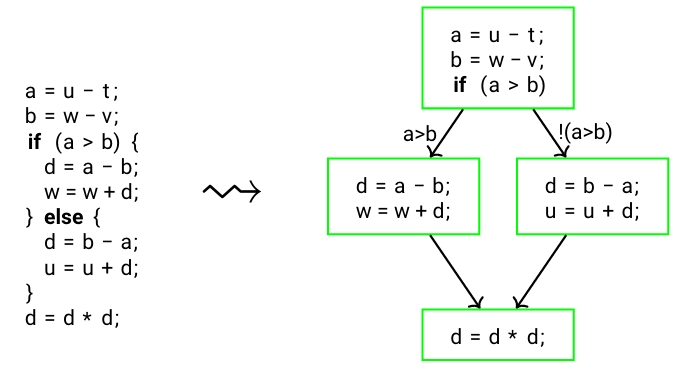
\includegraphics[width=1\textwidth]{Images/Contro-Flow Graph Example.jpeg}
\end{figure}
Path through CFG(P) from the \red{initial} to an \red{exit} node represents \red{one execution sequence} of P

\subsubsection*{Complex Control Flow}
\blue{Loops}

\begin{figure}[h]
    \centering
    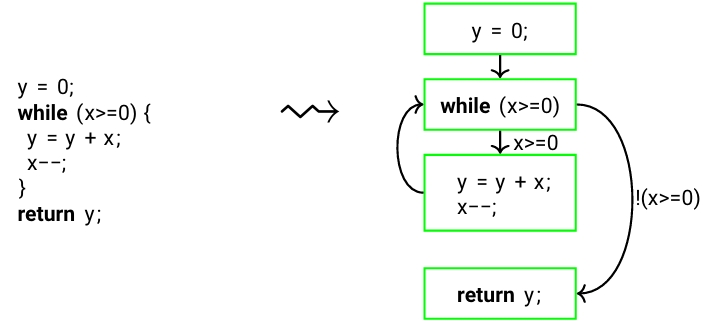
\includegraphics[width=0.9\textwidth]{Images/Loops.jpeg}
\end{figure}

Loop guard \red{not} in initial basic block: can be \red{independently} executed \\
\clearpage
\blue{Exeptions} 
\begin{figure}[h]
    \centering
    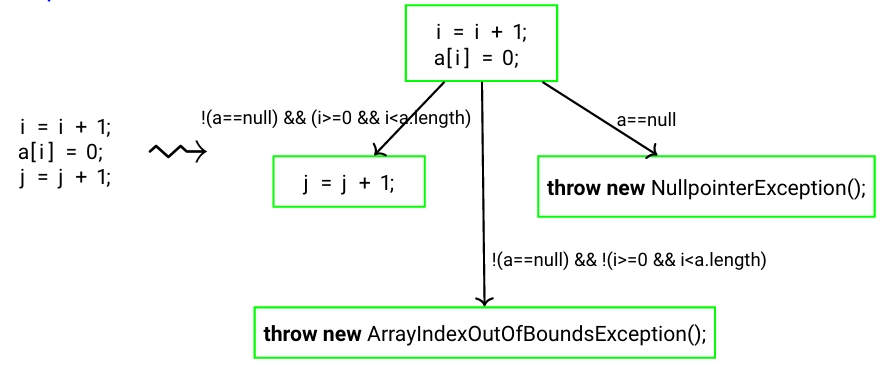
\includegraphics[width=0.9\textwidth]{Images/Exceptions.jpeg}
\end{figure}

Basic block ends, whenever a statement can throw an \red{exception} (branching) (Example also illustrates CFG with \red{multiple exit nodes})

\subsubsection*{Variant: Explicit Initial/Exit Nodes}
\begin{figure}[h]
    \centering
    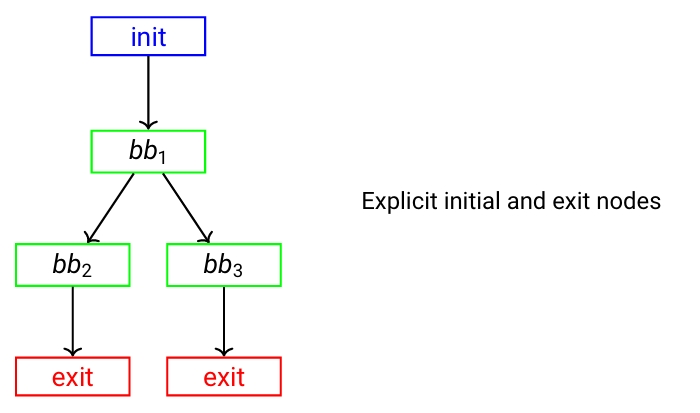
\includegraphics[width=0.9\textwidth]{Images/exit nodes.jpeg}
\end{figure}
\clearpage
\begin{figure}[h]
    \centering
    \includegraphics[width=0.9\textwidth]{Images/Variant: Explicit Initial-Exit Nodes.jpeg}
\end{figure}
\subsubsection*{Removal of Inactive Edges}
\begin{figure}[h]
    \centering
    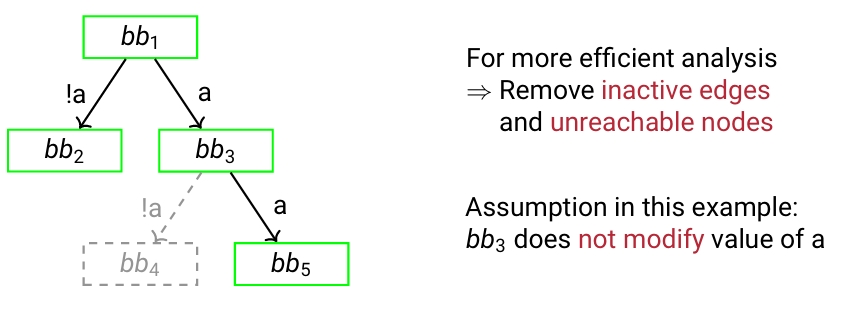
\includegraphics[width=0.9\textwidth]{Images/Removal of Inactive Edges.jpeg}
\end{figure}
\clearpage
\subsection{Code Metric: Cyclomatic Complexity}
\begin{figure}[h]
    \centering
    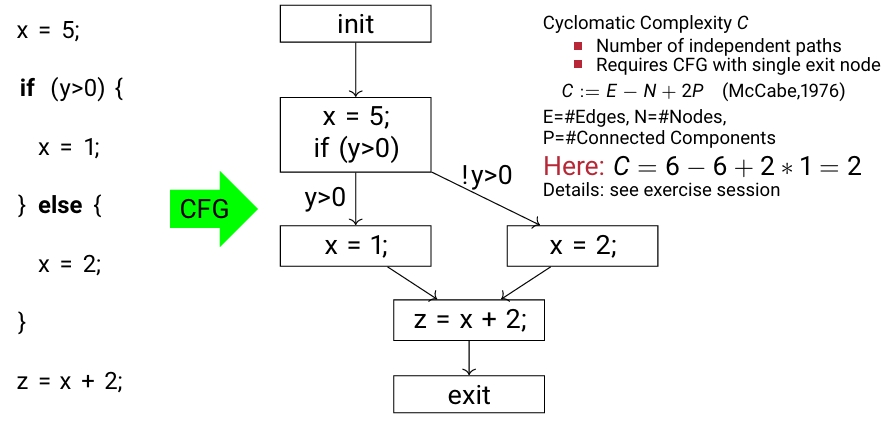
\includegraphics[width=0.9\textwidth]{Images/Cyclomatic Complexity.jpeg}
\end{figure}
\begin{defBox}
    \fatsf{Heuristics:} C>10 \red{rethink} design/coding to reduce complexity
\end{defBox}
\subsection{Code Measure: Class and Interface Coupling}
\begin{defBox}[title=Coupling...]
    ...indicates the amount of \red{dependence} between classes and packages
\end{defBox}
\begin{defBox}[title=Definition(Class and Interface Coupling)]
    A class or interface C is \red{coupled to a} class or interface D if C requires D directly or indirectly
\end{defBox}
\begin{itemize}
    \item A class that depends on 2 other classes has a \red{looser} coupling than a class that depends on 8 other classes
\end{itemize}
\begin{defBox}
    Like cyclomatic complexity, coupling is an \blue{evaluative} principle
\end{defBox}
\subsection{Common Occurences of Coupling in OOP}
\begin{itemize}
    \item Type X has an \red{attribute} that refers to a type Y
    \begin{codeBlock}{}
        class X {private Y y = ...}
        class X {private Y[] y = ...}
    \end{codeBlock}
    \item Type X contains a \red{(sub-)expression} of a type Y
    \begin{codeBlock}{}
        class X {private Object o = new Y();}
        class X {void m(){... if (o instanceof Y) ...}}
        class X {void m(){... x = o.a.count + 3; ...}} //where o.a is of type Y
    \end{codeBlock}
    \item A type X object \red{calls} methods of a type Y
    \begin{codeBlock}{}
        class X {void g(){Y.f();}}
        where class Y {static void f() {...}}
    \end{codeBlock}
    \item Type X \red{has a method that references} an instance of type Y (as method parameter, local variable, return type, ...)
    \begin{codeBlock}{}
        class X {X(Y y) {...}}
        class X {Y f() {...}}
        class X {void g() {Y y = ...;}}
        class X {void h() {Object o = new Y();}}
    \end{codeBlock}
    \item Type X is a \red{subtype} of type Y
    \begin{codeBlock}{}
        class Y {...}
        class X extends Y {...}
        class X implements Y {...}
    \end{codeBlock}
\end{itemize}
\subsection{Coupling in Java: An example}
\begin{codeBlock}{}
    package de.tud.simpletexteditor;
    import java.awt.event.ActionEvent;
    import java.awt.event.ActionListener;
    public class QuitAction implements ActionListener extends Object{
        @Override
        public void actionPerformed(ActionEvent e){
            System.exit(0);
        }
    }
\end{codeBlock}
Class \blue{QuitAction} is coupled directly with ...
\begin{itemize}
    \item ActionListener
    \item ActionEvent
    \item java.lang.Override
    \item java.lang.System
    \item java.lang.Object (any class in Java without an extends clause inherits directly from java.lang.Object)
\end{itemize}
\subsection{Design Principle: Avoid Tight Coupling, Avoid Very Loose Coupling}
\begin{infoBox}[title=Design-Prinzip: Vermeidung von starker Kopplung (aber nicht zu locker)]
    \begin{enumerate}
        \item \fatsf{Definition:}
        \begin{itemize}
            \item \fatsf{Starke Kopplung:} Klassen oder Komponenten sind stark voneinander abhängig, was dazu führt, dass Änderungen an einer Klasse viele anderen betreffen
            \item \fatsf{Lockere Kopplung:} Klassen/Komponenten haben minimale Abhängigkeiten und können unabhängig voneinander agieren, was Modularität und Wiederverwendbarkeit verbessert
        \end{itemize}
    \end{enumerate}
\end{infoBox}
\begin{infoBox}[title=Warum starke Kopplung problematisch ist:]
    \begin{itemize}
        \item \fatsf{Änderungskaskaden:} Änderungen an einer Klasse erfordern Änderungen in allen abhängigen Klassen
        \item \fatsf{Schwierige Verständlichkeit:} Stark gekoppelte Klassen sind schwer isoliert zu verstehen, da ihre Funktion von anderen abhängt
        \item \fatsf{Geringe Wiederverwendbarkeit:} Stark gekoppelte Klassen sind schwer in anderen Projekten einsetzbar, da immer auch die abhängigen Klassen benötigt werden
        \item \fatsf{Niedrige Modularität:} Starke Abhängigkeiten erschweren es, Teile des Systems zu isolieren und modular zu gestalten
    \end{itemize}
\end{infoBox}
\begin{infoBox}[title=Warum zu lockere Kopplung ebenfalls problematisch ist:]
    \begin{itemize}
        \item \fatsf{Grundprinzip der objektorientierten Programmierung (OOP):} OOP setzt auf Objekte, die miteinander kommunizieren. Zu wenig Kopplung führt zu isolierten Objekten, die nicht gut zusammenarbeiten
        \item \fatsf{Zentralisierung:} Übermäßig lockere Kopplung kann dazu führen, dass wenige \enquote{aktive} Objekte die gesamte Arbeit übernehmen müssen, was das System ineffizient und schwer wartbar macht
    \end{itemize}
\end{infoBox}
\begin{infoBox}[title=Der optimale Ansatz]
    \begin{itemize}
        \item Ziel ist eine \fatsf{lockere Kopplung}, die:
        \begin{itemize}
            \item Eine klare Kommunikation zwischen Klassen/Komponenten ermöglicht
            \item Klassen voneinander unabhängig macht, sodass sie leichter gewartet und wiederverwendet werden können
            \item Zentralisierte Arbeitslasten oder ineffiziente Strukturen vermeidet
        \end{itemize}
        \item \fatsf{Praktische Umsetzung:}
        \begin{itemize}
            \item Verwenden von \fatsf{Design-Patterns} wie Dependency Injection, Schnittstellen (Interfaces) oder das Observer-Pattern, um die richtige Balance zwischen Kopplung und Unabhängigkeit zu finden
        \end{itemize}
    \end{itemize}
\end{infoBox}
\subsection{Tight Coupling vs Loose Coupling}
\begin{defBox}
    Tight coupling to stable design elements and libraries is not a problem by itself (It still depends on the kind of elements to which it is coupled)
\end{defBox}
\begin{defBox}[title=Warning:]
    The quest for loose coupling to achieve reusability for a (hypothetical!) project may lead to \red{unnecessary complexity}\\
    Unwarranted decoupling can be one source of undue \red{class proliferation}: (\enquote{Ausuferung})\\
    Too many classes for the size of a given problem
\end{defBox}
\begin{infoBox}
    Starke Kopplung ist akzeptabel, wenn sie auf stabile, bewährte Elemente abzielt. Eine übermäßige Entkopplung hingegen kann zu unnötiger Komplexität und ineffizientem Design führen. Ziel ist ein ausgewogenes Verhältnis zwischen Kopplung und Entkopplung, das die tatsächlichen Anforderungen des Systems widerspiegelt
\end{infoBox}
\subsection{Class Proliferation: Classes vs. Object Roles}
\begin{defBox}[title=Two ways to model behavior]
    \red{As Class} with own attributes and operations\\
    \red{As Role} of an existing class, i.e. association\\
    \blue{When to create dedicated classes?}
\end{defBox}
\begin{infoBox}[title=Verhalten als eigene Klasse modellieren]
    \begin{itemize}
        \item \fatsf{Beschreibung:} Eine Klasse wird erstellt, die ihre eigenen Attribute und Operationen definiert
        \item \fatsf{Vorteile:}
        \begin{itemize}
            \item \fatsf{Kapselung:} Verhalten und zugehörige Daten sind in einer Einheit gebündelt
            \item \fatsf{Wiederverwendbarkeit:} Die Klasse kann in verschiedenen Kontexten verwendet werden
            \item \fatsf{Klarheit:} Die Klasse hat eine eindeutig definierte Rolle im System
        \end{itemize} 
        \item \fatsf{Wann verwenden?}
        \begin{itemize}
            \item Wenn das Verhalten \fatsf{komplex} ist oder eine \fatsf{unabhängige Existenz} rechtfertigt
            \item Wenn mehrere Objekte dieses Verhalten benötigen und es sich daher lohnt, es zentral zu definieren
            \item Beispiel: Eine Klasse PaymentProcessor für die Verarbeitung von Zahlungen
        \end{itemize}
    \end{itemize}
\end{infoBox}
\begin{infoBox}[title=Verhalten als Rolle einer bestehenden Klasse modellieren]
    \begin{itemize}
        \item \fatsf{Beschreibung:} Verhalten wird einer vorhandenen Klasse als Rolle zugeordnet, oft über eine Assoziation
        \item \fatsf{Vorteile:}
        \begin{itemize}
            \item \fatsf{Effizienz:} Vermeidet die Erstellung unnötiger Klassen
            \item \fatsf{Fokus:} Die bestehende Klasse bleibt zuständig für das Verhalten, das in ihrem Kontext relevant ist
        \end{itemize}
        \item \fatsf{Wann verwenden?}
        \begin{itemize}
            \item Wenn das Verhalten eng mit der vorhandenen Klasse verknüpft ist und keinen eigenständigen Kontext benötigt
            \item Wenn das Verhalten \fatsf{einfach} ist oder auf die Attribute der bestehenden Klasse zugreifen muss
            \item Beispiel: Ein Kunde hat die Rolle eines Bestellers, die durch eine Assoziation modelliert wird
        \end{itemize}
    \end{itemize}
\end{infoBox}
\begin{infoBox}[title=Entscheidungskriterien: Wann neue Klassen erstellen?]
    \begin{enumerate}
        \item \fatsf{Autonomie des Verhaltens:}
        \begin{itemize}
            \item Benötigt das Verhalten eine eigenständige Existenz mit klar abgegrenzten Operationen? $\rightarrow$ \fatsf{Neue Klasse}
        \end{itemize}
        \item \fatsf{Wiederverwendbarkeit:}
        \begin{itemize}
            \item Wird das Verhalten an mehreren Stellen im System benötigt? $\rightarrow$ \fatsf{Neue Klasse}
        \end{itemize}
        \item \fatsf{Komplexität:}
        \begin{itemize}
            \item Ist das Verhalten umfangreich oder kompliziert? $\rightarrow$ \fatsf{Neue Klasse}
        \end{itemize}
        \item \fatsf{Kohäsion:}
        \begin{itemize}
            \item Gehört das Verhalten zur Verantwortung der bestehenden Klasse? $\rightarrow$ \fatsf{Rolle einer Klasse}
        \end{itemize}
        \item \fatsf{Anpassungsfähigkeit:}
        \begin{itemize}
            \item Wird erwartet, dass sich das Verhalten unabhängig von der bestehenden Klasse ändert? $\rightarrow$ \fatsf{Neue Klasse}
        \end{itemize}
    \end{enumerate}
\end{infoBox}
\clearpage
\begin{figure}[h]
    \centering
    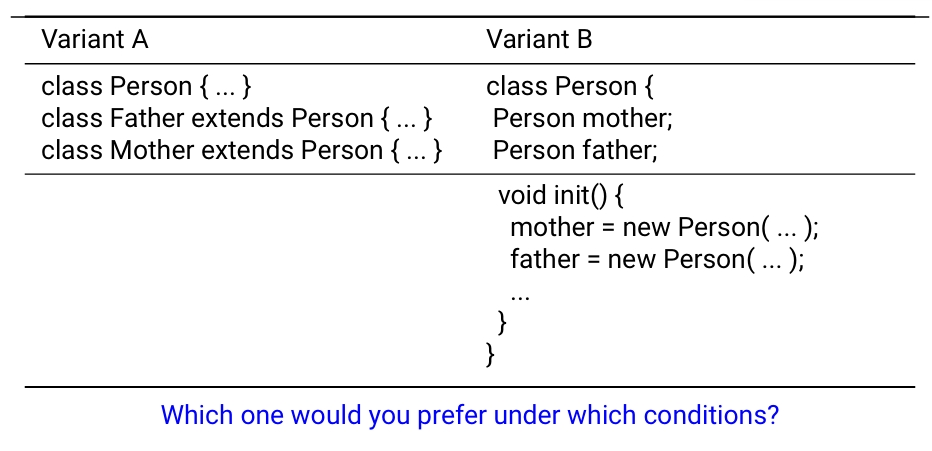
\includegraphics[width=0.9\textwidth]{Images/Class Proliferation.jpeg}
\end{figure}
\begin{itemize}
    \item \red{It depends on the domain model!}\\
    Do Mother/Father exhibit different behavior from Person?
    \item New classes should be warranted by truly \red{different behavior}
\end{itemize}
\subsection{Code Measure: Cohesion}
\begin{defBox}[title=Coheseion ...]
    ...measures the strength of the relation \red{among} elements of a class\\
    \blue{Motivation:}\\
    All operations and data within a class should \enquote{naturally belong} to the concept modelled by the class
\end{defBox}
\begin{defBox}
    Cohesion is an evaluative quality principle
\end{defBox}
\begin{infoBox}[title=Code Measure: Kohäsion (Cohesion)]
    \fatsf{Was ist Kohäsion?}\\
    Kohäsion misst, wie stark die Elemente einer Klasse (Methoden und Attribute) thematisch oder funktional zusammengehören. Eine hohe Kohäsion bedeutet, dass alle Elemente der Klasse sinnvoll miteinander verbunden sind und zu einer klar definierten Aufgabe beitragen
\end{infoBox}
\begin{infoBox}[title=Motivation für Kohäsion]
    \begin{itemize}
        \item \fatsf{Natürliche Zusammengehörigkeit:} Alle Operationen und Daten einer Klasse sollten sich auf das Konzept beziehen, das die Klasse modelliert
        \item \fatsf{Evaluatives Qualitätsprinzip:} Kohäsion wird verwendet, um die Qualität und Verständlichkeit von Klassen zu beurteilen
        \item \fatsf{Verbesserung der Modularität:} Klassen mit hoher Kohäsion sind leichter zu verstehen, zu warten und wiederzuverwenden
    \end{itemize}
\end{infoBox}
\begin{infoBox}[title=Typen von Kohäsion (nach Qualität geordnet)]
    \begin{enumerate}
        \item \fatsf{Zufällige (Coincidental) Kohäsion}
        \begin{itemize}
            \item \fatsf{Beschreibung:} Keine sinnvolle Beziehung zwischen den Elementen einer Klasse
            \item \fatsf{Beispiel:} Eine Klasse enthält Methoden und Daten, die nichts miteinander zu tun haben
            \item \fatsf{Bewertung:} Sehr schlecht. Sollte vermieden werden (außer bei Dienst- oder Utility-Klassen)
        \end{itemize}
        \item \fatsf{Temporale (Temporal) Kohäsion}
        \begin{itemize}
            \item \fatsf{Beschreibung:} Alle Elemente werden zur gleichen Zeit oder in einer bestimmten Reihenfolge ausgeführt
            \item \fatsf{Beispiel:} Initialisierungsmethoden, die nicht zusammenhängen, aber alle beim Start ausgeführt werden
            \item \fatsf{Bewertung:} Schlechte Praxis, da die Elemente keine thematische Verbindung haben
        \end{itemize}
        \item \fatsf{Sequentielle (Sequential) Kohäsion}
        \begin{itemize}
            \item \fatsf{Beschreibung:} Der Output einer Methode ist der Input für eine andere Methode
            \item \fatsf{Beispiel:} Eine Verarbeitungspipeline innerhalb einer Klasse
            \item \fatsf{Bewertung:} Mittel. Es gibt eine Beziehung zwischen den Elementen, aber die Verbindung ist rein sequentiell
        \end{itemize}
        \item \fatsf{Kommunikative (Communicational) Kohäsion}
        \begin{itemize}
            \item \fatsf{Beschreibung:} Alle Methoden der Klasse arbeiten mit denselben Eingabe- oder Ausgabedaten
            \item \fatsf{Beispiel:} Methoden, die verschiedene Operationen auf denselben Daten durchführen, z.B. eine Customer-Klasse mit Zugriff auf Kundendaten
            \item \fatsf{Bewertung:} Gut. Die Methoden teilen sich Daten und haben daher eine klare Verbindung
        \end{itemize}
        \item \fatsf{Funktionale (Functional) Kohäsion}
        \begin{itemize}
            \item \fatsf{Beschreibung:} Alle Elemente einer Klasse tragen dazu bei, eine einzige, klar definierte Verantwortung zu erfüllen
            \item \fatsf{Beispiel:} Eine Klasse PaymentProcessor, die ausschließlich für Zahlungsabwicklungen zuständig ist
            \item \fatsf{Bewertung:} Ideal. Dies ist der angestrebte Zustand
        \end{itemize}
    \end{enumerate}
\end{infoBox}
\subsection{Measuring Cohesion: Lack of Cohesion of Methods (LCOM)}
\begin{infoBox}[title=Was ist LCOM?]
    LCOM (Lock of Cohesion of Methdos) ist ein Indikator für die \fatsf{funktionale Kohäsion} einer Klasse. Es bewertet, wie stark die Methoden einer Klasse miteinander verbunden sind. Ein hoher LCOM-Wert deutet auf \fatsf{geringe Kohäsion} hin, was auf eine suboptimale Klassenstruktur hinweist.
\end{infoBox}
\begin{infoBox}[title=Definition (LCOM nach Li \& Henry)]
    Gegeben:
    \begin{itemize}
        \item C: Eine Klasse mit:
        \begin{itemize}
            \item F: Instanzfelder (Attribute)
            \item M: Methoden (außer Konstruktoren)
        \end{itemize}
    \end{itemize}
    \begin{enumerate}
        \item \fatsf{Graphenrepräsentation:}
        \begin{itemize}
            \item G(M, E): Ein ungerichteter Graph, in dem:
            \begin{itemize}
                \item M die Knoten (Methoden) sind
                \item E die Kanten zwischen Methoden darstellen
            \end{itemize}
            \item Es gibt eine Kante zwischen $m_{1}$ und $m_{2}$, wenn sie ein gemeinsames Feld f $\in$ F verwenden
        \end{itemize}
        \item \fatsf{LCOM-Wert}
        \begin{itemize}
            \item \fatsf{LCOM(C):} Anzaahl der \fatsf{zusammenhängenden Komponenten (Connected Components, CC)} im Graphen G
            \item Wertebereich: \fatsf{LCOM(C)$\in$[0, |M|]}, wobei:
            \begin{itemize}
                \item 0: Hohe Kohäsion (alle Methoden sind verbunden)
                \item |M|: Maximale Zerstreuung (jede Methode ist isoliert)
            \end{itemize}
        \end{itemize}
    \end{enumerate}
\end{infoBox}
\begin{infoBox}[title=Interpretation]
    \begin{itemize}
        \item \fatsf{Hoher LCOM-Wert:}
        \begin{itemize}
            \item Niedrige Kohäsion. Methoden sind unabhängig und teilen keine gemeinsamen Attribute
            \item Die Klasse könnte in mehrere kleinere Klassen aufgeteilt werden
        \end{itemize}
        \item \fatsf{Niedriger LCOM-Wert:}
        \begin{itemize}
            \item Hohe Kohäsion. Methoden arbeiten eng zusammen und sind durch gemeinsame Attribute verbunden
            \item Die Klasse repräsentiert klar ein Konzept
        \end{itemize}
    \end{itemize}
\end{infoBox}
\begin{infoBox}[title=Probleme und Herausforderungen der Formalisierung]
    \begin{enumerate}
        \item \fatsf{Sondermethoden:}
        \begin{itemize}
            \item Konstruktoren, toString(), hashcode(), und andere Standardmethoden beeinflussen LCOM, obwohl sie oft keine Kohäsionsprobleme darstellen
        \end{itemize}
        \item\fatsf{indirekte (transitive) Aufrufe:}
        \begin{itemize}
            \item Methoden könnten indirekt verbunden sein, was durch die einfach Definition von LCOM nicht erfasst wird
        \end{itemize}
        \item \fatsf{Datenzentrierung:}
        \begin{itemize}
            \item Der Fokus liegt nur auf der gemeinsamen Nutzung von Feldern. Methoden könnten jedoch kohäsiv sein, ohne dieselben Felder zu verwenden
        \end{itemize}
        \item \fatsf{Werteinterpretation:}
        \begin{itemize}
            \item Ein hoher Wert ist nicht immer schlecht; es hängt von der Funktionalität der Klasse ab
        \end{itemize}
    \end{enumerate}
\end{infoBox}
\subsection{Cohesion in Java: Example}
\begin{codeBlock}{}
    public class SimpleLinkedList{
        private final int value;
        private final SimpleLinkedList tail;
        public SimpleLinkedList(int v, SimpleLinkedList t){
            this.value = v; this.tail = t;
        }
        //methods
        public int geValue(){return value;}
        public SimpleLinkedList getTeil(){return tail;}
        public boolean contains(int searchFor){
            if (searchFor == value){return true;}
        return tail == null ? false : tail.contains(searchFor);
        }
    }
\end{codeBlock}
\begin{center}
    M = \{getValue, getTail, contains\}
\end{center}
\begin{figure}[h]
    \centering
    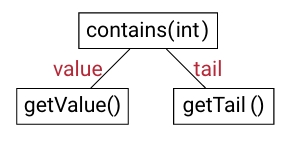
\includegraphics[width=0.5\textwidth]{Images/Cohesion in Java.jpeg}
\end{figure}
\begin{center}
    \begin{itemize}
        \item LCOM = 1 (of 3)
        \item High cohesion
        \item Maximal cohesion for intended behaviour
    \end{itemize}
\end{center}
\begin{codeBlock}{}
    import java.awt.Color;
    abstract class AbstractColorableFigure implements Figure{
        private Color lineColor = Color.BLACK;
        private Color fillColor = Color.WHITE;
        public Color getLineColor(){return lineColor;}
        public void setLineColor(Color c){lineColor = c;}
        public Color getFillColor(){return fillColor;}
        public void setFillColor(Color c){this.fillColor = c;}
    }
\end{codeBlock}
\begin{figure}[h]
    \centering
    \includegraphics[width=0.5\textwidth]{Images/Cohesion in Java: Example 2.jpeg}
\end{figure}
\begin{center}
    \begin{itemize}
        \item LCOM = 2 (of 4)
        \item Relatively low cohesion
        \item Reason:
        \begin{itemize}
            \item Conceptually independent attributes
            \item getter/setter methods
        \end{itemize}
        \item How to improve cohesion?
        \begin{itemize}
            \item Factor out common functionality from subclasses relted to color
            \item Maybe ColorableFigure is not a good abstraction
            \item Might be justifiable if several impementing subclasses exist
        \end{itemize}
    \end{itemize}
\end{center}
\subsection{Design Principle: Avoid Low Cohesion}
Classes with low cohesion are \red{undesirable}:
\begin{itemize}
    \item Hard to \red{comprehend}
    \item Hard to \red{reuse}
    \item Hard to \red{maintain} (easily affected by change)
    \item Typically represent \red{too coarse-grained abstraction}
    \item Often take responsibility that should have been \red{delegated}
\end{itemize}
\begin{defBox}
    \red{Observation:} Classes with high cohesion can often be described in a single sentence
\end{defBox}
\section{Part III: Responsibility-Driven Design}
\subsection{Designing Software Objects}
\subsubsection*{Responsibility-Driven Design}
\begin{defBox}
    A systematic approach to think about the \red{design} of software objects and components in terms of \red{responsiblities}, \red{roles} and \red{collaborations}
\end{defBox}
\begin{figure}[h]
    \centering
    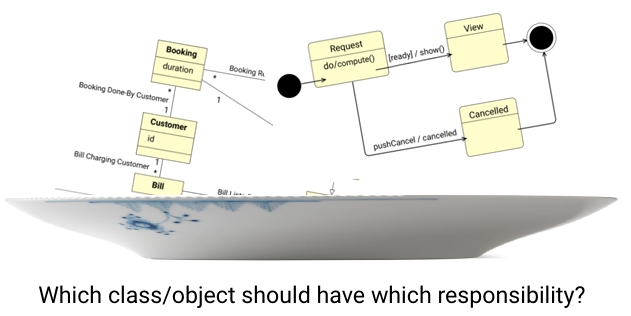
\includegraphics[width=1\textwidth]{Images/Responsibility.jpeg}
\end{figure}
\subsection{Responsibilities}
\begin{infoBox}[title=Definition und Bedeutung von Verantwortlichkeiten]
    \begin{itemize}
        \item Eine \fatsf{Verantwortlichkeit} repräsentiert eine Aufgabe oder Funktion, die einer Klasse in einem Softwaredesign zugewiesen wird
        \item Jede Verantwortlichkeit stellt eine mögliche \fatsf{Änderungsachse} dar:
        \begin{itemize}
            \item Wenn sich Anforderungen ändern, führen diese Änderungen oft zu einer Anpassung der entsprechenden Verantwortlichkeiten in den Klassen
        \end{itemize}
        \item Klassen mit \fatsf{mehreren Verantwortlichkeiten} haben \fatsf{mehrere Gründe}, sich zu ändern, was die Wartbarkeit und Stabilität des Codes verringert
    \end{itemize}
\end{infoBox}
\begin{infoBox}[title=Zitat von Robert C. Martin]
    \begin{itemize}
        \item \enquote{Jede Verantworltlichkeit ist eine Achse der Veränderung}
        \item \fatsf{Implikation:}
        \begin{itemize}
            \item Klassen sollten so entworfen sein, dass sie möglichst wenige Verantwortlichkeiten tragen. Dies minimiert die Notwendigkeit, mehrere Änderungen an einer Klasse vorzunehmen, wenn sich Anforderungen ändern
        \end{itemize}
    \end{itemize}
\end{infoBox}
\begin{infoBox}[title=Zuweisung von Verantwortlichkeiten]
    \begin{itemize}
        \item Das \fatsf{Zuweisen von Verantwortlichkeiten} ist ein zentraler Schritt im Code-Design
        \item Ziel: Klassen so gestalten, dass sie \fatsf{klar definiert und abgegrenzte Verantwortlichkeiten} haben
        \item \fatsf{Tools und Techniken zur Unterstützung:}
        \begin{itemize}
            \item \fatsf{Entwurfsmuster} (z.B. Singleton, Factory)
            \item \fatsf{Designprinzipien} (z.B. SOLID-Prinzipien)
            \item \fatsf{Idiome} (sprachspezifische Konventionen und Muster)
        \end{itemize}
    \end{itemize}
\end{infoBox}
\begin{infoBox}[title=Responsibility-Driven Design (RDD)]
    \begin{itemize}
        \item Im \fatsf{Responsibility-Driven Design} (RDD) liegt der Fokus auf der \fatsf{Definition von Verantwortlichkiten} und der Zuweisung dieser an Objekte
        \item \fatsf{Merkmale von RDD:}
        \begin{itemize}
            \item Softwareobjekte werden nicht nur als Datencontainer betrachtet, sondern als Einheiten, die \fatsf{Verantwortlichkeiten übernehmen}
            \item Verantwortlichkeiten können in zwei Kategorien unterteilt werden:
            \begin{enumerate}
                \item \fatsf{Was ein Objekt weiß} (Daten oder Zustände, die ein Objekt speichert)
                \item \fatsf{Was ein Objekt tut} (Funktionen oder Aktionen, die ein Objekt ausführt)
            \end{enumerate}
        \end{itemize}
        \item Verantwortlichkeiten werden in der \fatsf{Objektdesign-Phase} festgelegt, wobei Klassen und ihre Interaktionen im Mittelpunkt stehen
    \end{itemize}
\end{infoBox}
\subsection{Types of Responsibilities}
\begin{infoBox}[title=Grundtypen von Verantwortlichkeiten]
    \begin{enumerate}
        \item \fatsf{Doing Responsibilities (Tätigkeitsverantwortlichkeiten)}
        \begin{itemize}
            \item Diese beziehen sich auf die \fatsf{Ausführung von Aktionen}
            \item Beispiele für Tätigkeiten:
            \begin{itemize}
                \item Eine Aufgabe direkt ausführen (z.B. Berechnungen durchführen, Objekte erstellen)
                \item Eine Aktion in anderen Objekten initiieren
                \item Aktivitäten in anderen Objekten \fatsf{steuern} und \fatsf{koordinieren}
            \end{itemize}
            \item \fatsf{Beispiel:}
            \begin{itemize}
                \item Ein \fatsf{Rechnungsobjekt} (Bill) ist dafür verantwortlich, die Gesamtsumme der Rechnung zu berechnen
            \end{itemize}
        \end{itemize}
        \item \fatsf{Knowing Responsibilities (Wissensverantwortlichkeiten):}
        \begin{itemize}
            \item Diese beziehen sich auf das \fatsf{Wissen} eines Objekts und die Fähigkeit, Informationen bereitzustellen
            \item Arten von Wissen:
            \begin{itemize}
                \item \fatsf{Privates, gekapseltes Wissen} (z.B. interne Daten oder Attribute der Klasse)
                \item \fatsf{Beziehungen zu anderen Objekten} (z.B. Kenntnis über verbundene Objekte)
            \end{itemize}
            \item \fatsf{Beispiel:}
            \begin{itemize}
                \item Ein \fatsf{Auto-Objekt} (Car) ist dafür verantwortlich, die gefahrene Strecke zu kennen und bereitzustellen
            \end{itemize}
        \end{itemize}
    \end{enumerate}
\end{infoBox}
\subsection{Relation between Responsibilities and Methods}
\begin{infoBox}[title=Verantwortlichkeiten]
    \begin{itemize}
        \item Beschreiben \fatsf{höherwertige Aufgaben} oder Verpflichtungen, die eine Klasse oder ein Objekt innerhalb eines Softwaresystems übernhemen soll
        \item Eine Verantwortlichkeit kann:
        \begin{itemize}
            \item Durch eine einzige Methode in einem Objekt erfüllt werden
            \item Mehrere Methoden in einem Objekt erfordern
            \item Viele Methoden in mehreren Objekten einbeziehen
        \end{itemize}
        \item Verantwortlichkeiten sind \fatsf{konzeptionell} und dienen als Leitlinie für die Implementierung eines Verhaltens im System
    \end{itemize}
\end{infoBox}
\begin{infoBox}[title=Methoden]
    \begin{itemize}
        \item Sind die \fatsf{konkrete Implementierung} einer Verantwortlichkeit
        \item Sie definieren die spezifischen Aktionen, die ein Objekt ausführt, um seine Verantwortlichkeiten zu erfüllen
        \item Beispiel:
        \begin{itemize}
            \item \fatsf{Verantwortlichkeit:} \enquote{Verwalten einer Datenbankverbindung}
            \item \fatsf{Methode:} connect(), disconnect(), executeQuery()
        \end{itemize}
    \end{itemize}
\end{infoBox}
\begin{infoBox}[title=Wichtige Punkte]
    \begin{enumerate}
        \item \fatsf{Granularität von Verantwortlichkeiten:}
        \begin{itemize}
            \item \fatsf{Fein granulierte Verantwortlichkeiten} benötigen oft wenige Methoden (z.B. das Erstellen einer Rechnung)
            \item \fatsf{Grob granulierte Verantwortlichkeiten} können sich über viele Klassen und Methoden erstrecken (z.B. Zugriff auf eine Datenbank)
        \end{itemize}
        \item \fatsf{Verantwortlichkeiten $\neq$ Methoden:}
        \begin{itemize}
            \item Eine Verantwortlichkeit kann auf viele Methoden oder sogar auf mehrere Objekte verteilt sein
        \end{itemize}
    \end{enumerate}
\end{infoBox}
\subsection{Assigning Responsibilities to Mutiple Objects}
\begin{infoBox}[title=Verantwortlichkeiten auf mehrere Objekte verteilen]
    Bei der Zuweisung von Verantwortlichkeiten gibt es:
    \begin{itemize}
        \item \fatsf{Viele mögliche Ansätze}, was zu unterschiedlichen Designs führen kann:
        \begin{itemize}
            \item \fatsf{Gute Designs:} Wartbar, verständlich, wiederverwendbar und erweiterbar
            \item \fatsf{Schlechte Designs:} Fragile Systeme, die schwer zu warten und zu verstehen sind
        \end{itemize}
        \item Designprinzipien und Muster helfen, Verantwortlichkeiten \fatsf{effizient zuzuweisen}
    \end{itemize}
\end{infoBox}
\begin{infoBox}[title=Strategien für die Zuweisung von Verantwortlichkeiten]
    \begin{enumerate}
        \item \fatsf{Designprinzipien einhalten:}
        \begin{itemize}
            \item \fatsf{Single Responsibility Principle (SRP):} Jede Klasse sollte genau eine Verantwortlichkeit haben
            \item \fatsf{Kapselung (Encapsulation):} Daten und Methoden, die zusammengehören, sollten in einer Klasse bleiben
            \item \fatsf{Hohe Kohäsion, niedrige Kopplung:} Klassen sollten stark zusammenhängend sein, aber möglichst unabhängig von anderen
        \end{itemize}
        \item \fatsf{Designmuster nutzen:}
        \begin{itemize}
            \item Aufgaben an geeignete Objekte delegieren (z.B. Factory für die Objekterstellung, Repository für Datenbankzugriffe)
        \end{itemize}
        \item \fatsf{Wartbarkeit berücksichtigen:}
        \begin{itemize}
            \item Vermeiden, dass Objekte zu viele Verantwortlichkeiten übernehmen
            \item Verantwortlichkeiten logisch zuweisen, um Wiederverwendbarkeit zu fördern
        \end{itemize}
    \end{enumerate}
\end{infoBox}
\section{Part IV: More Design Principles}
\subsection{The Single Responsibility Principle (SRP)}
\enquote{A class should have only one reason to change}\\
\red{A responsibility is usually the primary reason for change}\\
$\Rightarrow$ One responsibility per class (the ideal to achieve)
\section{SRP: Rectangle Example}
\begin{figure}[h]
    \centering
    \includegraphics[width=1\textwidth]{Images/SRP: Rechtangle Example.jpeg}
\end{figure}
Does the Rectangle class follow the \red{Single Responsibility Principle}?\\
The Rectangle class hat \red{multiple} responsibilities:
\begin{itemize}
    \item \red{Calculate} the size of a rectangle: mathematical \red{model}
    \item \red{Render} rectangle on screen: \red{GUI} related functionality
\end{itemize}
Do you see any problems in having multiple responsibilities?
\begin{itemize}
    \item \red{Reuse} of Rectangle hindered b dependency on GUI package (GUI classes have to be deployed along with the Rectangle class)
    \item Any \red{change} in Graphical App causing a change of Rectangle requires to re-test and re-deploy Rectangle in the context of Geometry App
\end{itemize}
\subsection{Refactoring Rectangle to Satisfy SRP}
\begin{figure}[h]
    \centering
    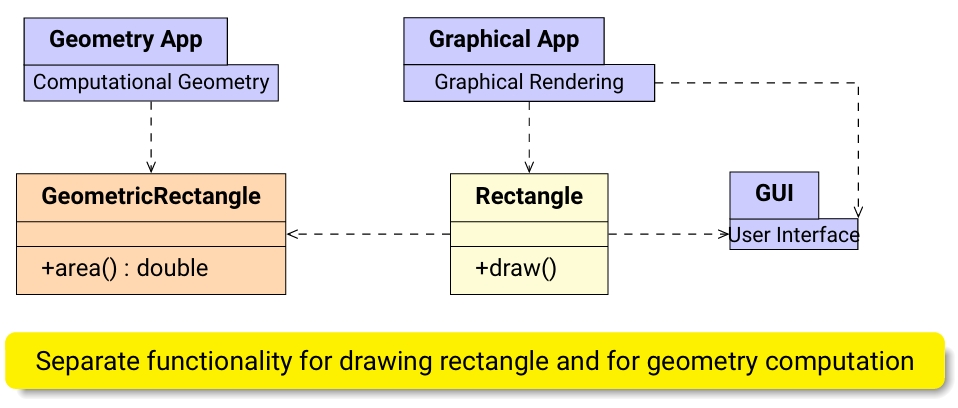
\includegraphics[width=1\textwidth]{Images/Refactoring Rectangle to Satisfy SRP.jpeg}
\end{figure}
\subsection{Collboration of Two Or More Classes}
\blue{Even if SRP is realized, not always clear, where to place a responsibility}
\begin{defBox}
    Designing a policy that requires \red{collaboration} of multiple classes
\end{defBox}
\begin{figure}[h]
    \centering
    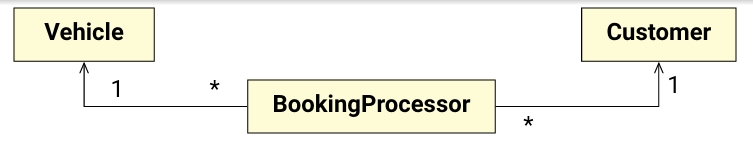
\includegraphics[width=1\textwidth]{Images/Collaboration of Two or More Classes.jpeg}
\end{figure}
\begin{itemize}
    \item \red{Vehicle:} Static Information about vehicle objects: number plate, verhicle class, most recent service, etc.
    \item \red{Customer:} Static information about customer: customer id, name, adress, allowed vehicle classes, etc.
    \item \red{BookingProcessor:} Static \& dynamic information about \red{one} requested booking: which vehicle, duration, who made it, etc.
\end{itemize}
\subsubsection*{Example}
\begin{defBox}[title=Task]
    Implement a check (\blue{checkPermision}) in BookingProcessor whether a customer is allowed to drive the chosen vehicle
\end{defBox}
\begin{defBox}[title=First design]
    \begin{enumerate}
        \item BookingProcessor queries Customer for allowed vehicle categories (calls \\ \blue{possibleCategories=customer.getVehicleCategories()})
        \item BookingProcessor passes vehicle categories to the chosen vehicle for checking (calls \\\blue{isPermitted=vehicle.checkPermission(possibleCategories)})
        \item BookingProcessor decides on outcome whether to continue processing or to reject the request
    \end{enumerate}
\end{defBox}
\begin{defBox}[title=Second design]
    \begin{enumerate}
        \item BookingProcessor queries Vehicle for vehicle categories (calls \blue{vehicleCategory=vehicle.getVehicleCategory()})
        \item BookingProcessor passes vehicle category to customer for checking (calls \\ \blue{isPermitted=customer.checkPermission(vehicleCategory))})
        \item BookingProcessor decides on outcome whether to continue processing or to reject the request
    \end{enumerate}
\end{defBox}
\begin{defBox}[title=Third design]
    \begin{enumerate}
        \item BookingProcessor queries Customer for allowed vehicle categories (calls \\ \blue{possibleCategories=customer.getVehicleCategories()})
        \item BookingProcessor queries Vehicle for vehicle category (calls \blue{vehicleCategory=vehicle.getVehicleCategory()})
        \item BookingProcessor implements check itself, hence, calls \blue{isPermitted=checkPermission(possibleCategories, vehicleCategory)}
        \item BookingProcessor decides on outcome whether to continue processing or to reject the request
    \end{enumerate}
\end{defBox}
\subsection{Delegation vs. Inheritance}
\begin{infoBox}[title=Delegation vs. Vererbung]
    Die Wahl zwischen Delegation und Vererbung ist ein entscheidender Designaspekt in der objektorientierten Programmierung. Hier ein Überblick über die beiden Ansätze, ihre Vor- und Nachteile sowie Richtilinien, wann welcher Ansatz sinnvoll ist.
\end{infoBox}
\begin{infoBox}[title=Vererbung]
    \fatsf{Definition:}
    \begin{itemize}
        \item Eine Klasse erbt von einer anderen Klasse
        \item Die abgeleitete Klasse übernimmt Attribute und Methoden der Basisklasse und kann diese erweitern oder überschreiben
    \end{itemize}
    \fatsf{Vorteile:}
    \begin{enumerate}
        \item \fatsf{Wiederverwendbarkeit:} Code der Basisklasse kann in Unterklassen direkt genutzt werden
        \item \fatsf{Einfache Implementierung:} Die Syntax (extends in Java) ist direkt und etabliert
        \item \fatsf{Konsistenz:} Alle Unterklassen teilen die gleiche Basislogik
    \end{enumerate}
    \fatsf{Nachteile:}
    \begin{enumerate}
        \item \fatsf{Unnatürliche Beziehungen:}
        \begin{itemize}
            \item Führt oft zu einer \enquote{ist-ein} Beziehung, auch wenn eine \enquote{hat-ein} Beziehung passender wäre
            \item Beispiel: Ein \fatsf{Kunde} ist nicht natürlich eine \fatsf{Authentifizierungsinstanz} sondern benötigt sie
        \end{itemize}
        \item \fatsf{Tiefer Vererbungsbaum:}
        \begin{itemize}
            \item Erhöht Komplexität und Wartung
            \item Kann zu fragile base class problem führen: Änderungen an der Basisklasse betreffen ungewollt alle Unterklassen
        \end{itemize}
        \item \fatsf{Verletzung des Single Responsibility Principle (SRP):}
        \begin{itemize}
            \item Eine Klasse übernimmt potenziell Verantwortlichkeiten, die sie nicht direkt betreffen
        \end{itemize}
        \item \fatsf{Unflexibel zur Laufzeit:}
        \begin{itemize}
            \item Vererbungsbeziehungen sind statisch und können nicht dynamisch geändert werden
        \end{itemize}
    \end{enumerate}
\end{infoBox}
\begin{infoBox}[title=Delegation]
    \fatsf{Definition:}
    \begin{itemize}
        \item Ein Objekt delegiert Aufgaben an ein anderes Objekt, das die erforderliche Funktionalität bereitstellt
        \item Beispiel: Statt dass die Klasse \fatsf{Customer} Authetifizierung direkt implementiert, ntutzt sie ein \fatsf{Authentication}-Objekt, um die Authentifizierung zu delegieren
    \end{itemize}
    \fatsf{Vorteil:}
    \begin{enumerate}
        \item \fatsf{Hohe Flexibilität:}
        \begin{itemize}
            \item Delegierte Objekte können zur Laufzeit geändert oder dyamisch erzeugt werden
        \end{itemize}
        \item \fatsf{Bessere Kapselung:}
        \begin{itemize}
            \item Jede Klasse bleibt auf ihre Kernaufgabe fokussiert, was das \fatsf{SRP} unterstützt
        \end{itemize}
        \item \fatsf{Leichte Wartbarkeit:}
        \begin{itemize}
            \item Änderungen an delegierten Code betreffen nur das Delegationsobjekt, nicht die Hauptklasse oder andere Delegierende
        \end{itemize}
        \item \fatsf{Geringere Kopplung:}
        \begin{itemize}
            \item Klassen sind weniger stark auseinander gebunden als bei Vererbung
        \end{itemize}
    \end{enumerate}
    \fatsf{Nachteile:}
    \begin{enumerate}
        \item \fatsf{Komplexere Implementierung}
        \begin{itemize}
            \item Zusätzliche Objekte und Interaktionen müssen eingeführt werden
        \end{itemize}
        \item \fatsf{Kein dedizierter Sprachsupport}
        \begin{itemize}
            \item Delegation muss manuell implementiert werden, während Vererbung direkt durch die Sprache unterstützt wird
        \end{itemize}
    \end{enumerate}
\end{infoBox}
\subsection{Implementing Delegation}
\begin{figure}[h]
    \centering
    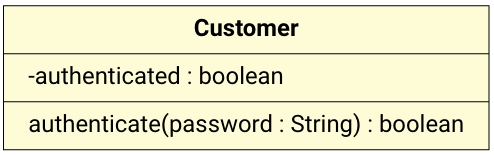
\includegraphics[width=1\textwidth]{Images/Implementing Delegation.jpeg}
\end{figure}
\begin{codeBlock}{}
    public class Customer{
        private boolean authenticated;
        public boolean authenticate(String password){
            authenticated = (Authentication.getAuthenticationToken(this)).authenticate(password);
            return authenticated;
        }
    }
\end{codeBlock}
\begin{infoBox}
    Hier:
    \begin{itemize}
        \item \fatsf{Customer} delegiert die Authentifizierung an ein \fatsf{Authentication}-Objekt
        \item Dadurch bleibt \fatsf{Customer} schlank und übernimmt nur die Aufgae, das Ergebnis zu speichern und zurückzugeben
    \end{itemize}
\end{infoBox}
\subsection{When to Use Delegation, When Inheritance?}
\begin{defBox}
    Inheritance must extend existing functionality \red{organically}
\end{defBox}
\blue{In many cases, delegation is preferable:}
\begin{itemize}
    \item Less intrusive on overall design, more focused
    \item Delegate can be changed/determined at runtime
\end{itemize}
\red{But:} No dedicated syntax like \fatsf{extends} in Java
\begin{defBox}[title=But isn't inheritance the essence of OO design?]
    No! The essence of OO is object \red{communication}, not inheritance!
\end{defBox}
\section{Part V: Encapsulation}
\subsection{Programming to Interfaces}
\begin{defBox}[title=Interface Concept]
    An \red{interface} declares the \blue{method signatures} and \blue{public constants} of its implementing classes
    \begin{itemize}
        \item Interfaces provide \red{independence} of functionality from implementation
    \end{itemize}
\end{defBox}
\begin{defBox}
    Always \enquote{\red{program to interfaces}}
\end{defBox}
\begin{defBox}[title=What does this mean?]
    \begin{itemize}
        \item Declare fields, return types, method parameters with \red{interface} type
        \item Do not expose \red{implementation details} in public methods
        \item Declare fields in implementing classes as \red{private}: use getters/setters
    \end{itemize}
\end{defBox}
\clearpage
\subsubsection*{Example}
\begin{figure}[h]
    \centering
    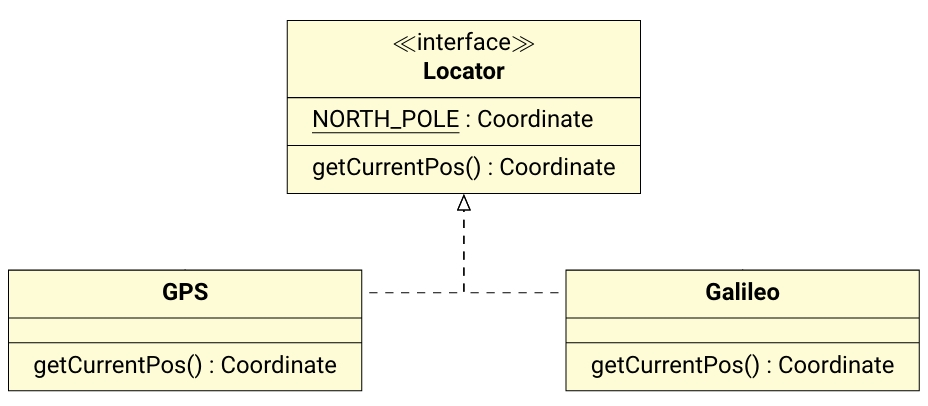
\includegraphics[width=0.9\textwidth]{Images/Programming to Interfaces 1.jpeg}
\end{figure}
\begin{figure}[h]
    \centering
    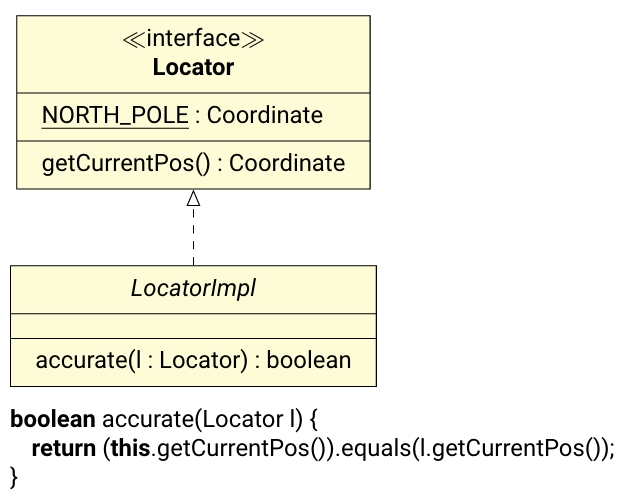
\includegraphics[width=0.6\textwidth]{Images/programmin to Interfaces 2.jpeg}
\end{figure}
\subsection{Programming to Interfaces: Advantages}
\begin{itemize}
    \item Helps to avoid \red{unjustified assumptions} about implementation
    \item Interfaces more \red{stable} than implementations
    \item To change implementation, sufficient to \red{exchange constructor}
    \begin{itemize}
        \item Can factor out implementation-independent code into abstract classes \blue{(as seen)}
        \item Reduces coupling (no dependence on implementing class)
    \end{itemize}
\end{itemize}
\subsection{Field Access}
\begin{defBox}
    \blue{Design principle:} make instance fields of classes \red{never} public
\end{defBox}
\begin{itemize}
    \item Breaks principle of \red{information hiding} and \red{programming to interfaces}:
    \begin{itemize}
        \item No distinction between implementation-specific and public data
        \item Implementation-specific details exposed to clients
    \end{itemize}
    \item \red{Brittle} code once field implementation changes
    \item Fields passed as arguments or aliased: hard to keep track of \red{dependencies} (coupling)
\end{itemize}
\begin{infoBox}
    Die Verletzung von \fatsf{Information Hiding und Programming to Interfaces} hat folgende Auswirkungen:
    \begin{enumerate}
        \item \fatsf{Fehlende Kapselung:} Änderungen in der Implementierung erfordern Änderungen im gesamten Client-Code
        \item \fatsf{Erhöhte Kopplung:} Schwer nachvollziehbare Abhängigkeiten zwischen Klassen entstehen
        \item \fatsf{Instabilität:} Der Code wird anfällig für Fehler und schwer wartbar
        \item \fatsf{Verlust der Kontrolle:} Direkte Manipulation von Feldern oder Objekten unterläuft die Verantwortung der Klasse
    \end{enumerate}
\end{infoBox}
\begin{defBox}[title=How to Access Fields of Other Objects?]
    Provide suitable \red{accessor} methods
    \begin{itemize}
        \item For field of type T named X: \blue{T getX() void setX(T x)}
    \end{itemize}
\end{defBox}
\subsection{Accessor Methods Exposing too Mush}
\begin{figure}[h]
    \centering
    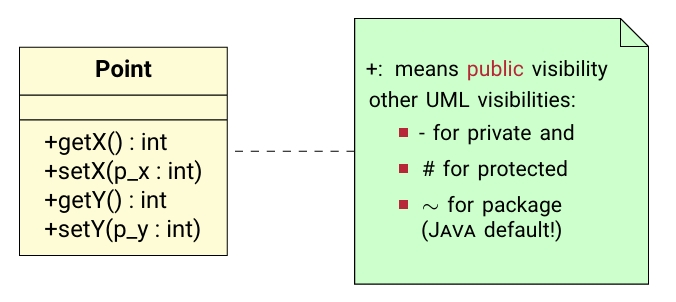
\includegraphics[width=0.6\textwidth]{Images/Point.jpeg}
\end{figure}
\blue{Class Point has public accessor operations}
\begin{itemize}
    \item Are there any problems with the above design of class Point?
    \item Does class Point expose too much implementation details to clients?
\end{itemize}
\begin{defBox}
    Accessor methods do \red{not necessarily} expose implementation details
\end{defBox}
\blue{But there is still an issue - What is it?}
\begin{itemize}
    \item Accessor methods may encourage poor encapsulation of \red{behavior}: Client accessing (x, y)-coordinates of \fatsf{Point} objects might implement behavior of points \red{not provided by} \fatsf{Point}
    \item Encourages misplacing \red{responsibilities}
\end{itemize}
\begin{infoBox}[title=Emfohlene Lösung: Methoden zur Kapselung von Verhalten]
    Anstatt Getter und Setter zu verwenden, sollte die Klasse die relevanten Operationen selbst implementieren, Beispiel:
    \begin{codeBlock}{}
        public class Point {
        private int x;
        private int y;
        // Konstruktor
        public Point(int x, int y) {
            this.x = x;
            this.y = y;
        }
        // Verhalten implementieren
        public void move(int dx, int dy) {
            this.x += dx;
            this.y += dy;
        }
        public double distanceTo(Point other) {
            int dx = this.x - other.x;
            int dy = this.y - other.y;
            return Math.sqrt(dx * dx + dy * dy);
        }
    
        @Override
        public String toString() {
            return "(" + x + ", " + y + ")";
        }
    }
    \end{codeBlock}
\end{infoBox}
\begin{infoBox}[title=Vorteile der verbesserten Kapselung]
    \begin{enumerate}
        \item \fatsf{Encapsulation (Bessere Kapselung):}
        \begin{itemize}
            \item Die Klasse Point ist vollständig verantwortlich für das Verhalten von Punkten
            \item Clients haben keinen direkten Zugriff auf interne Details
        \end{itemize}
        \item \fatsf{Reduced Coupling (Reduzierte Kopplung):}
        \begin{itemize}
            \item Änderungen an der internen Repräsentation von Point (z.B. Umstellung auf Polarkoordination) wirken sich nicht direkt auf den Client aus
        \end{itemize}
        \item \fatsf{Improved Responsibility Assignment (Bessere Verantwortungsverteilung):}
        \begin{itemize}
            \item Verhlaten wie Verschiebung oder Distanzberechnung bleibt innerhalb der Klasse, die die Daten enthält
        \end{itemize}
    \end{enumerate}
\end{infoBox}
\subsection{Accessor Methods for Private Fields: Generally Discourage?}
\begin{infoBox}
    Zugriffsmethoden (Getter und Setter) werden oft kritisiert, da sie interne Implementierungsdetails offenlegen und damit die Kapselung verletzen können. Dennoch gibt es bestimmte Szenarien, in denen sie gerechtfertigt und sogar notwendig sind. Hier eine Erklärung, wann und warum Zugriffsmethoden sinnvoll eingesetzt werden können:
\end{infoBox}
\begin{infoBox}[title=Notwendig für die Benutzeroberfläche (UI)]
    \begin{itemize}
        \item \fatsf{Szenario:} Wenn eine Klasse Daten repräsentiert, die in der Benutzeroberfläche angezeigt werden müssen, können Zugriffsmethoden einen kontrollierten Zugang zu den zugrunde liegenden Daten ermöglichen
        \item \fatsf{Grund:} Die UI benötigt oft die Rohdaten (z.B. Namen, Alter oder Koordination), um sie darzustellen, ohne direkt auf die interne Logik der Klasse zuzugreifen
        \item \fatsf{Beispiel:}
        \begin{codeBlock}{}
            public class User{
                private String name;
                public String getName(){
                    return name;
                }
            }
        \end{codeBlock}
        \begin{itemize}
            \item Die Methode getName ermöglicht der UI, den Namen des Nutzers anzuzeigen, ohne Zugriff auf die Implementierungsdetails der Klasse zu geben
        \end{itemize}
    \end{itemize}
\end{infoBox}
\begin{infoBox}[title=Durchsetzung von Regeln oder Richtlinien]
    \begin{itemize}
        \item \fatsf{Szenario:} Wenn eine Klasse bestimmte Regeln, Validierungen oder Richtlinien (z.B. Wertebereich oder berechnet Werte) implementieren muss, können Zugriffsmethoden diese Regeln durchsetzen
        \item \fatsf{Grund:} Zugriffsmethoden bieten eine kontrollierte Möglichkeit, Daten zu validieren oderzu verändern, ohne die Kapselung zu brechen
        \item \fatsf{Beispiel:}
        \begin{codeBlock}{}
            public class Account {
                private double balance;
                public double getBalance() {
                    return balance;
                }
                public void setBalance(double balance) {
                    if (balance < 0) {
                        throw new IllegalArgumentException("Das Guthaben darf nicht negativ sein.");
                    }
                    this.balance = balance;
                }
            }
        \end{codeBlock}
        \begin{itemize}
            \item Hier stellt die Methode setBalance sicher, dann kein negatives Guthaben erlaubt ist
        \end{itemize}
    \end{itemize}
\end{infoBox}
\begin{infoBox}[title=Statische Container ohne Verhalten]
    \begin{itemize}
        \item \fatsf{Szenario:} Wenn eine Klasse als einfacher Container für zusammengehörige, statische Daten oder Konstanten dient, können Zugriffsmethoden genutzt werden, um die Daten bereitzustellen
        \item \fatsf{Grund:} Die Klasse hat die Aufgabe, Daten zu speichern und bereitzustellen, sodass Zugriffsmethoden hier nicht der Intention widersprechen
        \item \fatsf{Beispiel:}
        \begin{codeBlock}{}
            public class Config {
                private static final String APP_NAME = "MeineApp";
                public static String getAppName() {
                    return APP_NAME;
                }
            }
        \end{codeBlock}
        \begin{itemize}
            \item Die Klasse Config dient als Container für unveränderliche Daten und bietet über Zugriffsmethoden Leserechte
        \end{itemize}
    \end{itemize}
\end{infoBox}
\begin{defBox}
    Make decisions \red{consciously} and be able to \red{justify} them (Not only here!)
\end{defBox}
\section{Applying Design Knowledge: The God Class Problem}
\subsection{The God Class Problem}
\begin{defBox}[title=God Classes]
    One class contains most of the system logic:
    \begin{itemize}
        \item Poorly distributed responsibilities
        \item Not an object-oriented design (collaborating objects)
    \end{itemize}
\end{defBox}
\subsection{Recognizing and Avoiding God Classes}
\begin{defBox}[title=Classes with unclear responsibilities]
    Class failing SRP\\
    \red{Required Action:} Split class and relocate responsibilities
\end{defBox}
\begin{defBox}[title=Classes with low cohesion\, non-communicating classes]
    Classes with methods operating on a small subset of its fields, not with other objects: \red{non-communicating behavior}\\
    \red{Required Action:} Split class and relocate responsibilities
\end{defBox}
\begin{defBox}[title=Uses classes with public field accessors]
    Can indicate that responsibilities are located in wrong class\\
    \red{Required Action:} Redesign interface and relocate responsibilities
\end{defBox}
\subsubsection*{Summary}
\begin{defBox}
    \red{Distribute} responsibilities uniformly among top-level classes in a design - Adherence to design principles reduces likelihood to create god class
\end{defBox}
\begin{defBox}[title=Sometimes design principles need to be traded off]
    Try to model the real world:\\
    \red{Low representational gap} facilitates maintenance and evolution\\
    \blue{But modelling the real world is not as important as the other principles}
\end{defBox}
\begin{defBox}[title=Example(Car)]
    In the real world, a car does not compute its next service interval\\
    In a car sharing system it is conceivable to assign responsibility for this to its corresponding class
\end{defBox}
\subsection{Design Principles}
\subsubsection*{Summary, Part I}
\begin{defBox}
    \begin{itemize}
        \item Avoid tight coupling of classes
        \item Avoid very loose coupling of classes
        \item Justify existence of classes by new behvior - consider roles
        \item Avoid low cohesion of classes
        \item Strive for single responsibility per class
        \item Use inheritance carefully, consider delegation
    \end{itemize}
\end{defBox}
\subsubsection*{Summary, Part II}
\begin{defBox}
    \begin{itemize}
        \item Avoid class proliferation (design too fine-granular)
        \item Program to interfaces
        \item Never make instance fields public, provide accessors if needed
        \item But: Provide only accessors needed for functionality
        \item Distribute functionalities evenly, avoid god classes
    \end{itemize}
\end{defBox}
\clearpage
\section{Design Techniques}
\blue{Techniques to implement} \red{design principles}
This lecture is about techniques to improve/establish
\begin{itemize}
    \item design and code \red{comprehensibility}
    \item \red{cohesion} by moving/reassigning responsibilities
\end{itemize}
In particular, we look at 
\begin{itemize}
    \item \red{Documentation}
    \item \red{Refactoring}
    \item \red{Design Patterns} 
\end{itemize}
\subsection{Part I: Documentation}
\subsubsection{Comprehensibility: Readability \& Documentation}
\begin{defBox}[title=Readability requires: ...]
    \begin{itemize}
        \item \red{Documentation} (explain design, architecture, ...relative to requirements)
        \item Source code \red{comments}:
        \begin{itemize}
            \item \red{API} documentation of each package, interface, class, method
            \item \red{Line} comments
        \end{itemize}
        \item Source \red{code}
    \end{itemize}
\end{defBox}
\begin{defBox}[title=Code Specific Aspects]
    \begin{itemize}
        \item Coding style \red{conventions} (on which line to write \{ ...)
        \item \red{Restrictions} on usage of language features (MISRA-C)
        \item Good \red{naming} of identifiers (classes, fields, methods, method parameters, local variables, etc.)
        \item Meaningful \red{comments}
    \end{itemize}
\end{defBox}
\subsubsection{Documentation: Commenting a Method Implementation}
\begin{defBox}
    How many lines of comment for method getImage()?
\end{defBox}
\clearpage
\subsubsection{Documentation: Example of a Java Source Code Comment}
\begin{figure}[h]
    \centering
    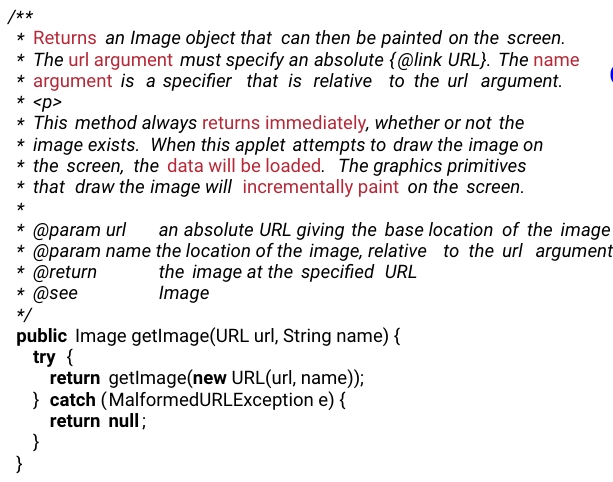
\includegraphics[width=1\textwidth]{Images/Example of a Java Source Code Comment.jpeg}
\end{figure}
\blue{Observations}
\begin{itemize}
    \item Length of source code vs. comment
    \item Comment adds \red{useful} information
    \begin{itemize}
        \item parameter format 
        \item behavior
        \item side effects
    \end{itemize}
    \item Comments rendered as HTML + keywords $\Rightarrow$ API documentation
\end{itemize}
\subsubsection{Documentation: Source Code Comments}
\blue{Two kinds of source code comments:}
\begin{itemize}
    \item (Public) \red{API} comment: class level and method level
    \item \red{Statement} level comments
\end{itemize}
\begin{defBox}[title=API comments]
    \red{Intent:} API usage documentation\\
    \red{Audience:} Third-party developers using the code as framework/library\\
    Describe in detail \red{when} method may be called and its \red{behavior}:
    \begin{itemize}
        \item Additional restrictions on parameters besides type (e.g., not null reference or non-negative)
        \item Side-effects on object state
        \item When and which exceptions are thrown
    \end{itemize}
\end{defBox}
\begin{infoBox}[title=API-Kommentare: Eine Übersicht]
    API-Kommentare dienen als Dokumentation für Drittentwickler, die eine Codebasis als Framework oder Bibliothek verwenden. Sie stellen sicher, dass Entwickler die Methoden korrekt nutzen und verstehen, welche Bedingungen erfüllt sein müssen und welche Auswirkungen die Methoden haben können.
\end{infoBox}
\begin{infoBox}[title=Ziel(Intent):]
    \begin{itemize}
        \item \fatsf{Dokumentation der Nutzung} der API für Entwickler
        \item Sicherstellen, dass Entwickler wissen, \fatsf{wann} und \fatsf{wie} eine Methode aufgerufen werden kann
    \end{itemize}
\end{infoBox}
\begin{infoBox}[title=Zielgruppe(Audience):]
    \begin{itemize}
        \item \fatsf{Drittentwickler}, die die API oder Bibliothek nutzen, aber keinen direkten Zugriff auf den internen Code haben
    \end{itemize}
\end{infoBox}
\begin{infoBox}[title=Wichtige Inhalte von API-Kommentaren:]
    \begin{enumerate}
        \item \fatsf{Wann eine Methode aufgerufen werden kann:}
        \begin{itemize}
            \item Kontext des Aufrufs(z.B. muss eine Verbindung hergestellt sein)
            \item Lebenszyklusbedingungen (z.B. nach Initialisierung, vor dem Schließen eines Objekts)
        \end{itemize}
        \item \fatsf{Verhalten der Methode:}
        \begin{itemize}
            \item Welche Aktion wird ausgeführt?
            \item Welche Änderungen treten auf?
        \end{itemize}
        \item \fatsf{Zusätzliche Einschränkungen für Parameter:}
        \begin{itemize}
            \item Anforderungen, die über den Datentyp hinausgehen:
            \begin{itemize}
                \item \fatsf{Nicht-null-Referenzen:} Der Parameter darf nicht null sein
                \item \fatsf{Wertebereiche:} Zahlenwerte müssen positiv oder in einem bestimmten Bereich sein
            \end{itemize}
        \end{itemize}
        \item \fatsf{Nebenwirkungen auf den Objektzustand:}
        \begin{itemize}
            \item Welche Felder oder Zustände des Objekts ändern sich nach dem Methodenaufruf?
        \end{itemize}
        \item \fatsf{Ausnahmen(Exceptions):}
        \begin{itemize}
            \item Wann und warum eine Methode eine Ausnahme auslöst
            \item Typen von Ausnahmen und deren Bedeutung
        \end{itemize}
    \end{enumerate}
\end{infoBox}
\begin{defBox}[title=Statement level comments]
    \red{Intent:} Describe implementation details, structure code\\
    \red{Audience:} Developers on the same code base\\
    Should be \red{concise} and used sparingly
    \begin{itemize}
        \item Clear and well-wirtten code is-to an extent-self-documenting
        \item Might be an indication of overly complex code\\
        $\Rightarrow$ \fatsf{Refactor!}
    \end{itemize}
\end{defBox}

\subsection{Part II: Refactoring}
\subsubsection{Refactoring: Definition}
\enquote{\red{Refactoring} is a disciplined technique for restructuring an existing body of code, altering its internal structure \blue{without changing its external behavior}}
\begin{defBox}[title=Objectives]
    \begin{itemize}
        \item \red{Preparing} addition of new features (\red{not} addition of new features)
        \item Improving design, for example, increasing \red{cohesion}
        \item Increasing \red{comprehensibility}
        \item Improving \red{maintainability} of the software
    \end{itemize}
\end{defBox}
\subsubsection{Refactoring: Reasons to Refacor Design and Code}
\begin{defBox}
    Assume we want to add a feature for querying cars with certain number of seats
\end{defBox}
\begin{codeBlock}{}
    public class Query{
        List<Car> cars;
        public List<Car> cars;
        public List<Car> getCarsOfModel(String model){
            List<Car> filteredCars = new LinkedList<>();
            for(Car c : cars){
                if(model.equals(c.getModel())){
                    filteredCars.add(c);
                }
            }
            return filteredCars;
        }
    }
\end{codeBlock}
\blue{Addition of New Features}\\
Restructureing makes \red{adding new feature easier:}
\begin{itemize}
    \item Less code duplication
    \item Avoid nested conditions, etc.
\end{itemize}
\begin{defBox}
    Quick and dirty: Copy \& Paste\\
    \blue{Disadvantages:}
    \begin{itemize}
        \item Code duplication
        \item No support for future extensions (other query types)
    \end{itemize}
\end{defBox}
\begin{codeBlock}{}
    public class Query{
        public List<Car> cars;
        public List<Car> getCarsOfModel(String model){...}
        public List<Car> getCarsWithSeats(int seats){
            List<Car> filteredCars = new LinkedList<>();
            for(Car c : cars){
                if(c.getSeats() == seats){
                    filteredCars.add(c);
                }
            }
            return filteredCars;
        }
    }
\end{codeBlock}
\begin{defBox}
    \red{Parameterize} method with property \red{f} to filter as a new argument\\
    Filtering for car properties now flexible:\\
    \blue{filterCars(Car::getModel, \enquote{Golf})}\\
    or\\
    \blue{filterCars(Car.:getSeats, 5)}
\end{defBox}
\begin{codeBlock}{}
    public class Query{
        List<Car> cars;
        public <T>List<Car> filterCars(Function<Car, T> f, T value){
            List<Car> filteredCars = new LinkedList<>();
            for(Car c : cars){
                if(value.equals(f.apply(c))){
                    filteredCars.add(c);
                }
            }
            return filteredCars;
        }
    }
\end{codeBlock}
\begin{figure}[h]
    \centering
    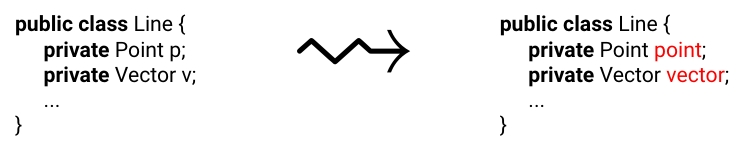
\includegraphics[width=0.75\textwidth]{Images/Reasons to Refactor Design and Code.jpeg}
\end{figure}
\blue{Comprehensibility}\\
Restrucuring makes design or code easier to understand:
\begin{itemize}
    \item Choose meaningful names for variables, methods, ...
    \item Simplify unnecessarily convoluted program logic
\end{itemize}
\clearpage
\subsubsection{Refactoring Techniques}
\subsubsection*{Example: A Statistics Class for CaSh}
\begin{figure}[h]
    \centering
    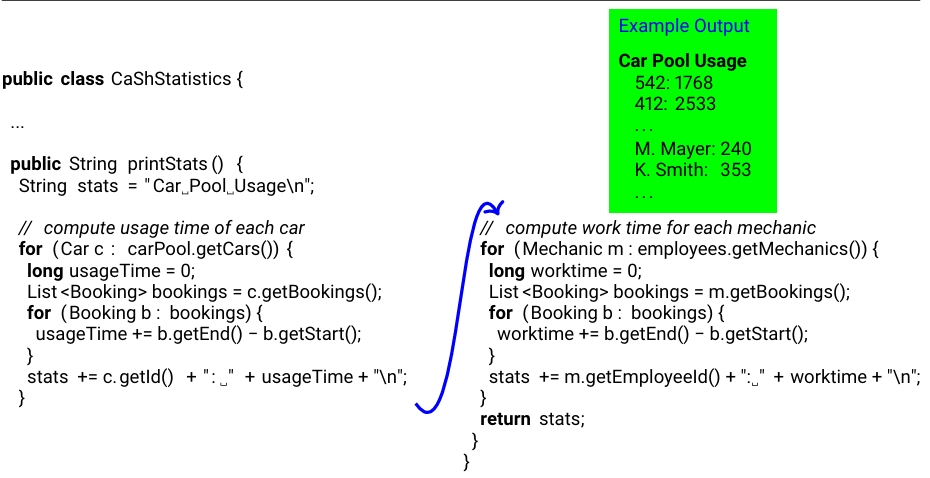
\includegraphics[width=1\textwidth]{Images/A Statistics Class for Cash.jpeg}
\end{figure}
\subsubsection*{Extract Method}
\begin{defBox}[title=When to Use?]
    \begin{itemize}
        \item One Method does several things (Computers usage time, work time and composes statistics)
        \item Similar functionality realized within one or as part of several methods
    \end{itemize}
\end{defBox}
\begin{defBox}[title=Extract Method]
    \begin{enumerate}
        \item Create new method (target)
        \item Copy extracted code to target
        \item Identify set of local variables used in extracted code
        \begin{enumerate}
            \item Variables only used in extracted code declared as local variables
            \item Exactly one local variable modified: check if target method can be query
            \item More than one local variable modified: Extract Method not applicable
            \item Pass undeclared local variables as method arguments
        \end{enumerate}
        \item Replace extracted code in refactoring source with call to extracted method
    \end{enumerate}
\end{defBox}
\begin{codeBlock}{}
    public class CaShStatistics{
        ...
        public String printStats(){
            String stats = "Car Pool Usage\n";
            //compute usage time of each car
            for (Car c : carPool.getCars()){
                long usageTime = computeCarUsageTime(c);
                stats += c.getId() + ": " + usageTime + "\n";
            }
            //compute work time for each mechanic
            ...
        }
        private long computeCarUsageTime(Car c){
            long usageTime = 0;
            List<Booking> bookings = c.getBookings();
            for (Booking b : bookings){
                usageTime += b.getEnd() - b.getStart();
            }
            return usageTime;
        }
    }
\end{codeBlock}
Applying \red{Extract Method} twice
\begin{defBox}[title=Observation 1]
    \blue{usageTime, worktime} only used \red{once}\\
    $\Rightarrow$ Apply refactoring \red{Inline Temp}
\end{defBox}
\begin{defBox}[title=Observation 2]
    Improve readability by extracting methods for printing usage time \& worktime \red{and} call usage methods from there
\end{defBox}
\begin{defBox}[title=Observation 3]
    Comments in printStats() do not add anything useful any more $\Rightarrow$ Remove
\end{defBox}
\begin{codeBlock}{}
    public class CaShStatistics{
        ...
        public String printStats(){
            String stats = "Car Pool Usage\n"
            stats = printCarUsageTime(stats);
            stats = printMecahnicsWorktime(stats);
            return stats;
        }
        private String printCarUsageTime(String s){...}
        private String printMecahnicsWorktime(String s){...}
        private long computeCarUsageTime(Car c){...}
        private long computeWorktime(Mechanic m){...}
    }
\end{codeBlock}
\subsubsection*{Move Method-Improving Cohesion}
\begin{codeBlock}{}
    public class CaShStatistics{
        ...
        private long computeCarUsageTime(Car c){
            long usageTime = 0;
            List<Booking> bookings = c.getBookings();
            for (Booking b : bookings){
                usageTime += b.getEnd() - b.getStart();
            }
            return usageTime;
        }
        private String printCarUsageTime(String s){...}
    }
\end{codeBlock}
\red{Cohesion got worse!}\\
computeCarUsageTime(), computeWorktime() do not use \red{fields} of class CaShStatistics (not even methods)\\
\blue{Make them static?} Not a good Solution in this case\\
\blue{Problem at the core:} \red{CaShStatistics has too many responsibilities}\\
Method computeCarUsageTime() \red{belongs actually to} Car (similarly computeworktime() to Mechanic)\\
$\Rightarrow$ Use refactoring \red{Move Method}
\begin{defBox}[title=Applicability Check for Move Method]
    Does the source method (here: \blue{computeCarUsageTime()})
    \begin{itemize}
        \item use features of the source class (here: CaShStatistics)?
        \item override a method or is overriden by a subclass?
    \end{itemize}
    If answer is no, then \red{Move Method} is applicable\\
    (otherwise other refactorings/preparation may first be necessary, see M. Fowler, \enquote{Refactoring})
\end{defBox}
\begin{defBox}[title=Applying Move Method]
    \begin{enumerate}
        \item \red{Declare} method in target class
        \item Copy source method to target class and \red{adjust} method to work there
        \item Determine how to reference target object from source (\red{delegation})
        \item Turn source method into \red{delegating} method
        \item Source method may be \red{removed} if not needed, also \red{accessors} in target class
    \end{enumerate}
\end{defBox}
\begin{codeBlock}{}
    public class CaShStatistics{
        ...
        private String printCarUsageTime(String s){
            for (Car c : carPool.getCars()){
                s += c.getId() + ": " + c.getUsageTime() + "\n";
            }
            return s;
        }
    }
    public class Car{
        ...
        public long getUsageTime(){
            long usageTime = 0;
            List<Booking> bookings = this.getBookings();
            for(Booking b : bookings){
                usageTime += b.getEnd() - b.getStart();
            }
            return usageTime;
        }
    }
\end{codeBlock}
\subsubsection*{Extract Class}
\begin{defBox}[title=Refactoring Extract Class]
    Apply \red{Extract Class}, if a class has two or more independent responsibilities and no other class is suitable to move the corresponding fields and methods\\
    Like \fatsf{Move Method}, improves cohesion, more generally applicable
\end{defBox}
\begin{defBox}[title=Applying Extract Class]
    \begin{enumerate}
        \item \red{Create} new class
        \item \red{Link} new class from old clas, may need new \red{accessor} method
        \item Apply refacotring \red{Move Field} (not shown)
        \item Apply refactoring \red{Move Method}
        \item Review and reduce class interfaces (unnecessary accessors ...)
    \end{enumerate}
\end{defBox}
\begin{figure}[h]
    \centering
    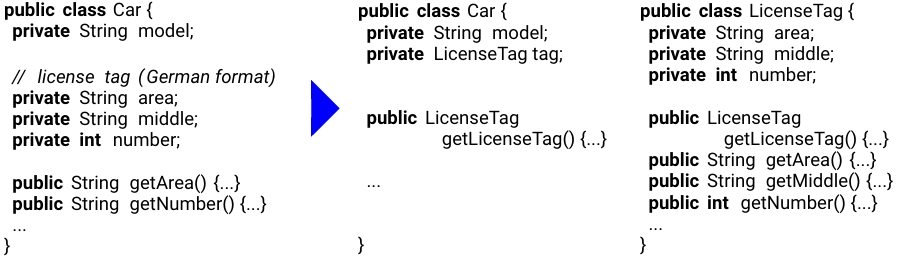
\includegraphics[width=1\textwidth]{Images/Extract Class.jpeg}
\end{figure}
\subsection{Part III: Design Patterns-Introduction}
\subsubsection{Design Patterns}
A \red{design pattern} describes ...
\begin{itemize}
    \item a \red{problem} that \red{reoccurs} regularly in our domain,
    \item is the core of a \red{solution} to that problem, such that one can reuse this solution many times, never in exactly the same way
\end{itemize}
\blue{Motivation}
\begin{itemize}
    \item Designing reusable software is \red{hard}
    \item Novices are \red{overwhelmed}
    \item Experts draw from \red{experience}
    \item Some design solutions \red{reoccur}
\end{itemize}
\blue{Understanding reoccuring solutions has different facets}
\begin{itemize}
    \item Know \red{when} to apply
    \item Know the \red{consequences} (trade-offs)
\end{itemize}
\subsubsection{Some Remarks on Software Patterns}
\begin{itemize}
    \item Software design patterns are part of the \red{current software practice}
    \begin{itemize}
        \item Used and implemented in APIs+documentation (Java Standard Library)
    \end{itemize}
    \item \red{Criticism:} Lack of scientific evaluation on effects of design patterns
    \begin{itemize}
        \item Some studies even indicate averse effects for certain patterns
        \item Further inverstigations of the underlying reasons necessary
    \end{itemize}
    \item Standard book: Erich Gamma et al., \red{Design Patterns: Elements of Reusable Object-Oriented Software}, Addision-Wesley/Pearson, 1994
    \item Cf. code \red{building blocks} at different levels of abstraction\\
    \red{Below Design Patterns:} \blue{Idiom} (Coplien, 1991)\\
    \red{Above Design Patterns:} \blue{Architectural Patterns}(Buschmann et al., 1996) (see Lecture 5)
\end{itemize}
\subsubsection{Idioms}
\begin{itemize}
    \item \red{Not} design patterns
    \item Limited size and (often) specific to programming language
\end{itemize}
\begin{defBox}[title=Example]
    \blue{String Copy in C:} while (*d++ = *s++); (s, d are char arrays)\\
    \blue{Lazy instantiation of Singletons} (uses \red{Double-chicked Locking Idiom}:)
    \begin{codeBlock}{}
        private static volatile Device device = null;
        public static Device instance(){
            Device result = device;
            if (result == null){
                synchronized(Device.class){
                    result = device;
                    if (result == null){device = result = new Device();}
                }
            }
            return result;
        }
    \end{codeBlock}
\end{defBox}
\subsubsection{A First Design Pattern: Template Method}
\begin{defBox}[title=Design Goal]
    Implement an algorithm in a manner that allows one to \red{adapt} specific and well-defined subfunctions in order to realize \red{variants}
\end{defBox}
\begin{figure}[h]
    \centering
    \includegraphics[width=1\textwidth]{Images/A First Design Pattern: Templete Method.jpeg}
\end{figure}

\subsubsection{The Template Method Pattern}
\begin{figure}[h]
    \centering
    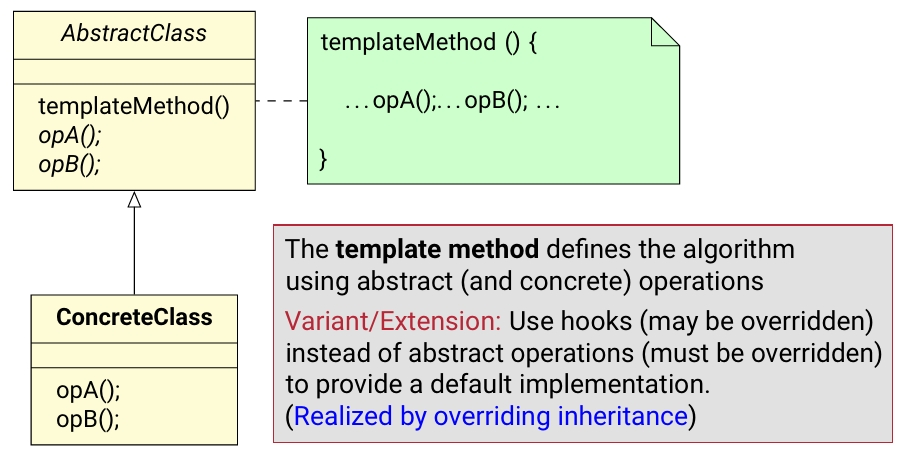
\includegraphics[width=1\textwidth]{Images/The Template Method Pattern.jpeg}
\end{figure}
\begin{defBox}[title=Benefits of the Template Method Pattern]
    \begin{itemize}
        \item \red{Separation} of variant and invariant parts
        \item Avoidance of \red{code duplication} in subclasses (commom behavior is factored out)
        \item Control of subclass \red{extensions}
    \end{itemize}
\end{defBox}

\subsection{Part IV: Design Patterns-General Properties}
\subsubsection{Design Patterns: Benefits \& Essentials}
\blue{Benefits}\\
\red{Systematic} (software) development:
\begin{itemize}
    \item \red{Document} expert knowledge
    \item \red{Reuse} of general and good solutions that worked well before
    \item Raising the \red{abstraction level} of code/documentation
\end{itemize}
\blue{Essentials}
\begin{itemize}
    \item A pattern has a \red{name}
    \item The adressed problem (and its solution) is \red{relevant} (problem occurs regularly, not a one-off problem)
    \item The solution can be easily \red{adapted} to a variant of the problem
\end{itemize}
\begin{defBox}
    A \red{Design Pattern} describes a solution for a problem in a context
\end{defBox}
\subsubsection{Essential Elements of a Software Design Pattern}
\red{Pattern Name} Short mnemonic to extend the design vocabulary\\
\red{Problem Description}
\begin{itemize}
    \item \red{When} to apply the pattern
    \item Conditions under which the pattern provides a \red{solution}
\end{itemize}
\red{Solution}
\begin{itemize}
    \item \red{Elements} constitution the design 
    \item \red{Relationships}, \red{responsibilities}, \red{collaborations} amon these elements
\end{itemize}
\red{Consequences} Trade-offs of applying the pattern, for example:
\begin{itemize}
    \item Language and implementation issues
    \item \red{Impact} on flexibility, extensibility, or portability
\end{itemize}
\subsubsection{Template for a Design Pattern}
\begin{figure}[h]
    \centering
    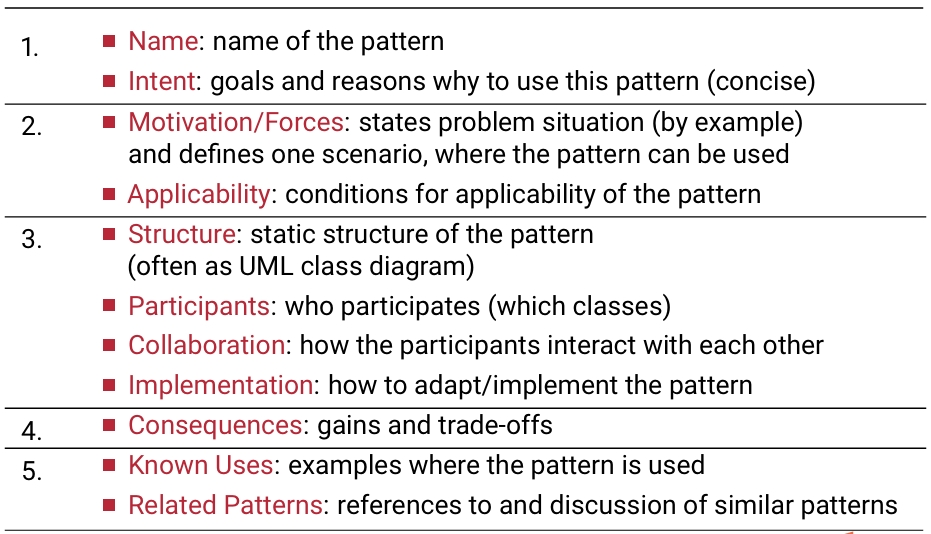
\includegraphics[width=1\textwidth]{Images/Template for a Design Pattern.jpeg}
\end{figure}
\clearpage
\subsubsection{Design Patterns Serve Multiple Purposes}
\begin{figure}[h]
    \centering
    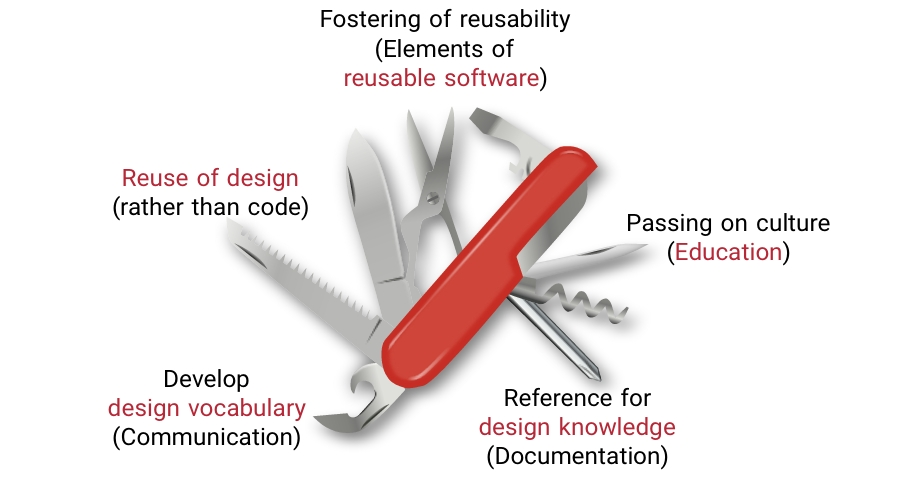
\includegraphics[width=1\textwidth]{Images/Design Patterns Serve Multiple Purposes.jpeg}
\end{figure}
\begin{defBox}
    Patterns aim to enable construcation of high-quality software architectures
\end{defBox}
\begin{defBox}
    Software design patterns describe 
    \begin{itemize}
        \item commonly recurring structures of interacting software components
        \item that solve general design problems within a particular context
    \end{itemize}
\end{defBox}
\subsubsection{Occurrences of Design Patterns Outside Software}
\blue{Some usages of design patterns:}
\begin{itemize}
    \item \red{Chess:} from rules to expertise
    \item \red{Agriculture:} wisdom vs. science
    \item \red{Architecture:} pioneering work on design patterns by \blue{C. Alexander}
\end{itemize}
\clearpage
\section{Design Patterns}
\subsection*{UML Class Diagram Reference for Design / Implementation Phase}
\begin{figure}[h]
    \centering
    
\includegraphics[width=0.9\textwidth]{Design Pattern Images/UML Class Diagram Reference 1.jpeg}
\end{figure}
\begin{figure}[h]
    \centering
    
\includegraphics[width=0.9\textwidth]{Design Pattern Images/UML Class Diagram Reference 2.jpeg}
\end{figure}
\begin{figure}[h]
    \centering
    
\includegraphics[width=0.9\textwidth]{Design Pattern Images/UML Class Diagram Reference 3.jpeg}
\end{figure}
\begin{figure}[h]
    \centering
    
\includegraphics[width=0.9\textwidth]{Design Pattern Images/UML Class Diagram Reference 4.jpeg}
\end{figure}
\clearpage
\subsection{Part I: Behavioural Design Patterns: Observer Pattern}
\subsubsection{Observer Pattern: Motivation, Example}
\begin{figure}[h]
    \centering
    \includegraphics[width=0.9\textwidth]{Design Pattern Images/Observer Pattern: Motivation.jpeg}
\end{figure}
\subsubsection{Consequence of OO Design}
\begin{defBox}
    OOAD (Object-Oriented Analysis und Design) divides a problem into manageable \red{subtasks}
\end{defBox}
\begin{defBox}
    $\Rightarrow$ Objects are responsible for \red{subtasks}\\
    They \blue{collaborate} to accomplish complex tasks
\end{defBox}
\fatsf{Advantages:}
\begin{itemize}
    \item Each object easy to implement, understand, maintain, reuse
    \item \blue{Divide-and-conquer} approach to design possible
    \item Flexible combinations from different collaborations possible
    \item \blue{Versatility}
\end{itemize}
\fatsf{Disadvantages:}
\begin{itemize}
    \item Behavior is \red{distributed} across multiple objects
    \item \blue{Lack of clarity}(\enquote{Unübersichtlichkeit}) of \red{overall} design
    \item Any state change of one object may affect many others
    \item \blue{Interdependence}
\end{itemize}
\subsubsection{Desirable: Communication with Low Coupling}
\begin{defBox}[title=Change Propagation]
    \begin{itemize}
        \item \red{Change propagation} (of object states) can be \red{hard wired}, but this couples objects together and diminishes their flexibility and potential for reuse
        \item A flexible way is neded to allow objects to \red{inform each other about changes without strongly coupling them}
    \end{itemize}
\end{defBox}
\begin{defBox}[title=Representative Scenario]
    Separation of GUI from underlying data, such that classes defining application data and presentations can be \red{reused independently}
\end{defBox}
\begin{defBox}[title=Task]
    \red{Decouple} a data model (\blue{\enquote{subject}}) from parties (\blue{\enquote{observers}}) interested in changes of its internal state
\end{defBox}
\begin{defBox}[title=Requirements]
    \begin{itemize}
        \item \red{Subject} should not need to know details about its \red{observers}
        \item Identity and number of observers \red{not predetermined} or fixed
        \item \red{New observer} kinds can be added to the system \red{dynamically}
        \item \red{Polling} is an inappropritate (inefficient) communication pattern
    \end{itemize}
\end{defBox}
\begin{defBox}
    Fundamental problem: one-to-many communication relation among objects
\end{defBox}
\subsubsection{Observer Pattern: Pattern Structure}
\begin{figure}[h]
    \centering
    \includegraphics[width=0.9\textwidth]{Design Pattern Images/ObserverPattern:Pattern Structure.jpeg}
\end{figure}
\begin{defBox}
    Methods getState(), modifyState() of ConreteSubject are placeholders for implementing methods of a concrete subject that get or modify its state
\end{defBox}
\begin{infoBox}[title=Wie funktioniert das Observer Pattern?]
    \begin{enumerate}
        \item \fatsf{Subject (Subjekt)}\\
        Das Subject ist das Objekt, das überwacht wird. Es verwaltet eine Liste von Beobachtern und stellt Methoden bereit, um:
        \begin{itemize}
            \item Beobachter hinzufügen (\textsf{attach} oder \textsf{subscribe})
            \item Beobachter zu entfernen (\textsf{detach} oder \textsf{unsubscribe})
            \item Beobachter über Änderungen zu benachrichtigen (\textsf{notifyObservers})
        \end{itemize}
        \item \fatsf{Observer (Beobachter)}\\
        Ein Observer ist ein Objekt, das am Zustand des Subjekts interessiert ist. Es definiert eine Methode (\textsf{update}), die aufgerufen wird, wenn das Subjekt seinen Zustand ändert
        \item \fatsf{ConcreteSubject (Konkretes Subjekt)}\\
        Das konkrete Subjekt implementiert die Schnittstelle oder Basisklasse des Subjects. Es enthält den eigentlichen Zustand und die Logik zur Verwaltung der Beobachter
        \item \fatsf{ConcreteObserver (Konkreter Beobachter)}\\
        Der konkrete Beobachter imlementiert die Observer-Schnittstelle. ER definiert, wie er auf Zustandsänderungen des Subjekts reagiert
    \end{enumerate}
\end{infoBox}
\begin{infoBox}[title=Ablauf des Observer Patterns]
    \begin{enumerate}
        \item Der Beobachter (Observer) registriert sich beim Subjekt (Subject), um Benachrichtigungen zu erhalten
        \item Das Subjekt ändert seinen Zustand und ruft die Methode \textsf{notifyObservers()} auf
        \item Das Subjekt informiert alle registrierten Beobachter, indem es deren \textsf{update}-Methode aufruft
        \item Die Beobachter reagieren auf die Benachrichtigung und passen sich entsprechend an
    \end{enumerate}
\end{infoBox}
\subsubsection{Observer Pattern: Example}
\begin{figure}[h]
    \centering
    \includegraphics[width=0.9\textwidth]{Design Pattern Images/Observer Pattern: Example.jpeg}
\end{figure}
\subsubsection{Observer Pattern: Adding and Removing Observers}
\begin{codeBlock}{}
    public abstract class Subject{
        private CopyOnWriteArrayList<Observer> observers = new CopyOnWriteArrayList<>();
        public void attach(Observer obs){
            if (obs == null){
                throw new IllegalArgumentException();
            }
            observers.addIfAbsent(obs);
        }
        public void detach(Observer obs){
            if (obs == null){
                throw new IllegalArgumentException();
            }
            observers.remove(obs);
        }
        public void notifyObservers(){...}
    }
\end{codeBlock}
\begin{defBox}[title=Remarks]
    \begin{itemize}
        \item Observers are added and removed from a list of observers
        \item Attention: In amulti-threaded environment additional care is necessary, for instance, synchronization and/or use of thread-safe data structures (here: CopyOnWriteArrayList)
    \end{itemize}
\end{defBox}
\subsubsection{Observer Pattern: Change Notification}
\begin{figure}[h]
    \centering
    \includegraphics[width=0.9\textwidth]{Design Pattern Images/Observer Pattern: Change Notification.jpeg}
\end{figure}
\subsubsection{Abstract Coupling}
\begin{defBox}
    Observer pattern realizes \red{abstract coupling} between subject and observers
\end{defBox}
\begin{defBox}[title=Abstract Coupling]
    \begin{itemize}
        \item Implementation of \blue{attach(), detach(), notify()} operations need to know only observer \red{interface}
        \begin{itemize}
            \item No coupling to observer \red{implementation}
        \end{itemize}
        \item Observers can be added and removed \red{dynamically}
    \end{itemize}
\end{defBox}
\subsubsection{Observer Patterns: Consequences}
\begin{defBox}[title=Advantages]
    \begin{itemize}
        \item \red{Abstract coupling} between \blue{Subject} and \blue{Observer}
        \item Support for \red{broadcast communication} \enquote{ausstrahlen} (as opposed to polling):
        \begin{itemize}
            \item \blue{notifyObservers()} does not specify its receivers
            \item Sender does not know the (concrete) type of the receiver
        \end{itemize}
    \end{itemize}
\end{defBox}
\begin{defBox}[title=Disadvantages and Limitations (control over updates)]
    \begin{itemize}
        \item Danger of \red{update cascades} to observers and their dependent objects
        \item Update sent to \red{all observers}, but not \red{all} might be interested in \red{any} change
        \item \red{No change details}\\
        $\Rightarrow$ Observers need to find out what has changed
        \item \red{Uniform interface} for all observer updates:\\
        $\Rightarrow$ Subject cannot send optional parameters to observers
    \end{itemize}
\end{defBox}
\subsubsection{Model-View-Controller by Example}
\begin{figure}[h]
    \centering
    
\includegraphics[width=0.9\textwidth]{Design Pattern Images/Model-View-Controller by Example.jpeg}
\end{figure}
\subsubsection{Concrete Subject Implementation}
\begin{codeBlock}{}
    public class CarInventory extends Subject{
        private List<Car> carPool = new ArrayList<>();
        ...
        public void addCar(Car c){
            if (!carPool.contains(c)){
                carPool.add(c);
            }
            notifyObservers();
        }
        public void removeCar(Car c){
            carPool.remove(c);
            notifyObservers();
        }
    }
\end{codeBlock}
\begin{itemize}
    \item \blue{CarInventory} is the ConcreteSubject
    \item Methods addCar(), removeCar() change ConcreteSubject's state
    \item Change notification of registered observers via notifyObserver()
    \item Update notification takes from o.update(this)
\end{itemize}
\subsubsection{Observer Update Example}
\begin{codeBlock}{}
    public class CarInventoryView extends JFrame implements Observer{
        ...
        public CarInventoryView(CarInventory inventory){
            ...
            inventory.attach(this);
            fillTable(inventory);
            ...
        }
        @Override
        public void update(Subject subject){
            fillTable((CarInventory) subject);
        }
        private void fillTable(Carinventory inventory){
            ...
            inventory.getCars().forEach(c -> model.addRow(...));
        }
        ...
    }
\end{codeBlock}
\blue{CarInventoryView}
\begin{itemize}
    \item is a ConcreteObserver
    \item implements Observer interface
    \begin{itemize}
        \item update(Subject) called by notifyObserver() of concrete Subject CarInventory, knows \red{inventory}
        \item update() causes full table refresh
    \end{itemize}
\end{itemize}
\subsubsection{Implementation Alternatives I: Who Informs Observers of State Change?}
\begin{enumerate}
    \item State changing methods notify observers (as seen)
    \begin{codeBlock}{}
        class CarInventory extends Subject{
            List<Car> pool = new LinkedList<Car>();
            public void removeCar(Car c){
                pool.remove(c);
                notifyObservers();
            }
            ...
        }
    \end{codeBlock}
    \begin{infoBox}
        Beobachter werden sofort bei jeder Änderung benachrichtigt. Dies ist einfach zu implementieren, kann jedoch ineffizient sein, wenn viele Änderungen in kurzer Zeit stattfinden.
    \end{infoBox}
    \item Client triggers update
        \begin{codeBlock}{}
            class Subject {
                private List<Observer> observers = new ArrayList<>();
                public void addObserver(Observer observer) {
                    observers.add(observer);
                }
                public void notifyObservers() {
                    for (Observer observer : observers) {
                        observer.update();
                    }
                }
            }
            interface Observer {
                void update();
            }
            class CarInventory extends Subject {
                private List<Car> pool = new LinkedList<>();
                public void removeCar(Car c) {
                    pool.remove(c); // Keine automatische Benachrichtigung
                }
                public void addCar(Car c) {
                    pool.add(c); // Keine automatische Benachrichtigung
                }
            }
            class Car {}
            class InventoryObserver implements Observer {
                @Override
                public void update() {
                    System.out.println("Inventory updated!");
                }
            }
            // Hauptprogramm
            public class Main {
                public static void main(String[] args) {
                    CarInventory inventory = new CarInventory();
                    InventoryObserver observer = new InventoryObserver();
                    inventory.addObserver(observer);
            
                    Car car1 = new Car();
                    Car car2 = new Car();
            
                    // Der Client führt mehrere Änderungen aus
                    inventory.addCar(car1);
                    inventory.addCar(car2);
                    inventory.removeCar(car1);

                    // Der Client löst die Benachrichtigung aus
                    inventory.notifyObservers();
                }
            }
        \end{codeBlock}
        Die Methode notifyObservers() wird vom Client nach Abschluss der Änderungen aufgerufen. Dadurch wird nur eine einzige Benachrichtigung gesendet, auch wenn mehrere Änderungen durchgeführt werden
\end{enumerate}
\begin{defBox}
    \red{Advantage (of 1.)}\\
    \begin{itemize}
        \item Close to actual subject state change
        \item Observers will be reliably notified
    \end{itemize}
    \red{Disadvantage (of 1.)}
    \begin{itemize}
        \item If several changes performed at once, then each triggers notification: Causing, for example, many screen refreshes
    \end{itemize}
\end{defBox}
\subsubsection{Implementation Alternatives II: Passing Update Information}
\begin{enumerate}
    \item \red{Pull Mode} (as seen)
    \begin{codeBlock}{}
        public class CarInventoryView implements Observer{
            @Override
            public void update(Subject subject){
                fillTable((CarInventory) subject);
            }
        }
    \end{codeBlock}
    \begin{itemize}
        \item \blue{Concrete observer queries}
        \item \blue{concrete subject for change}
        \item Often too coarse gained, anything might be changed (Here: full table content refresh)
    \end{itemize}
    \begin{infoBox}
        Im Pull-Modus ruft der Beobachter (Observer) die Informationen über Änderungen direkt beim Subjekt (Subject) ab, wenn er über eine Änderung benachrichtigt wird. Das Sujekt gibt keine spezifischen Details zur Änderung weiter.\\
        \fatsf{Eigenschaften:}
        \begin{itemize}
            \item Der Beobachter fragt den vollständigen Zustand des Subjekts ab (z.B. das gesamte Auto-Inventar)
            \item Geeignet für einfache Szenarien, aber möglicherweise ineffizient, da der gesamte Zustand unabhängig von der Art der Änderung neu geladen wird
            \item \fatsf{Nachteil:} Änderungen sind oft zu grobgranular, was unnötige Operationen (z.B. vollständige Tabellenaktualisierung) verursachen kann
        \end{itemize}
    \end{infoBox}
    \item \red{Push Mode}
    \begin{codeBlock}{}
        public class CarInventoryView implements Observer{
            @Override
            public void update(Subject subject, Change e){
                if (e.getKind() == Change.CarDeletion){
                    deleteRowForCar(e.getCar());
                } else {
                    ...
                }
            }
        }
    \end{codeBlock}
    \begin{itemize}
        \item Change aspect \blue{parameter} of update()
        \item Makes efficient view update possible
    \end{itemize}
    \begin{infoBox}
        Im Push-Modus sendet das Subjekt spezifische Informationen über die Änderung an den Beobachter. Der Beobachter kann die Änderung effizient verarbeiten, ohne den gesamten Zustand des Subjekts abzufragen\\
        \fatsf{Eigenschaften:}
        \begin{itemize}
            \item Das Subjekt sendet detaillierte Informationen zur Änderung (z.B. Art der Änderung und betroffene Daten)
            \item Ermöglicht dem Beobachter, die Änderung effizient zu verarbeiten (z.B. nur eine Zeile aktualisieren oder entfernen)
            \item \fatsf{Vorteil:} Präzise und effizient, besonders bei großen oder komplexen Daten
        \end{itemize}
    \end{infoBox}
\end{enumerate}
\subsubsection{Implementation Alternatives III: Concrete Subject with Subclass Hierarchy}
\begin{codeBlock}{}
    class ComplexSubject extends Subject{
        Object o = new Object();
        public void trickyChange(){
            o = new Object(); // not so tricky ...
            notifyObservers();
        }
    }
    class MoreCmplexSubject extends ComplexSubject{
        Object anotherO = ...;
        @Override
        public void trickyChange(){
            super.trickyChange(); //causes notification
            another() = ...;
            notifyObservers(); //another notification
        }
    }
\end{codeBlock}
\blue{Problem:}\\
Invocation of trickyChange() on ComplexSubject causes \red{premature notification}, because of call to super.trickyChange() in super class
\begin{codeBlock}{}
    class ComplexSubject extends Subject{
        Object o = new Object();
        public void trickyChange(){
            doTrickyChange();
            notifyObservers();
        }
        protected void doTrickyChange(){
            o = new Object();
        }
    }
    class MoreCmplexSubject extends ComplexSubject{
        Object anotherO = ...;
        @Override
        public void trickyChange(){
            super.doTrickyChange(); //avoid notification
            another() = ...;
        }
    }
\end{codeBlock}
\blue{Solution:}\\
Separate logic for model change and notification invocation into different methods (use \red{Template Method Pattern})
\subsubsection{Implementation Alternatives IV: Specifying Modifications of Interest}
\blue{Specify relevant aspect of model when registering observer}
\begin{itemize}
    \item \blue{addObserver(Observer, Aspect):} 
    Aspect encodes the kind of events of interest for \red{that} Observer
    \item In case of a state change, subject calls \blue{triggerUpdatefor(anAspect)} on itself, which informs all observers that are registered for anAspect
\end{itemize}
\blue{Different observer interfaces for different aspects} (common JAVA use case)
\begin{itemize}
    \item Different \red{observer interfaces} are available\\
    For example: \blue{ActionListener, MouseListener}
    \item Subject \red{informs} listeners on changes they are interested in\\
    For example: Mouse click on a button
    \item Subject provides \red{registration methods} for supported listener interfaces \\
    For example: \blue{addMouseListener(MouseListener)}
    \item Observers implement \red{listener interfaces} (often inner classes of view)
\end{itemize}
\subsection{Part II: Creational Pastterns: Factory Method}
\subsubsection{Factory Method: Motivation, Example}
Assume we develop a \red{framework} for appliccations that can present \red{multi-format documents} to the user\\
Need to support a wide variety of application software:
\begin{itemize}
    \item Text editor 
    \item Word processor
    \item Vector drawing 
    \item document Viewer, ...
\end{itemize}
\begin{defBox}
    The framework must be able to manage \red{different} kinds of documents with \red{common}
\end{defBox} 
\clearpage
\subsubsection{Common Functionality for Document Management}
\begin{figure}[h]
    \centering
    
\includegraphics[width=0.9\textwidth]{Design Pattern Images/Common Functionality for Document Management.jpeg}
\end{figure}
\subsubsection{Factory Method: Intent, Example}
\begin{defBox}
    Declare \red{interface for object creation}, let subclasses decide class to instantiate: Factory Method lets an application class \red{defer instantioation} to subclasses
\end{defBox}
\begin{infoBox}[title=Intent (Absicht)]
    Das \fatsf{Factory Method Pattern} ermöglicht einer Klasse, die Instanziierung ihrer Objekte an Unterklassen zu delegieren. Das Hauptziel ist, eine \fatsf{Schnittstelle für die Objekterstellung} bereitzustellen, ohne dass die konkrete Klasse, die instanziiert wird bekannt sein muss. Dadurch wird der Code flexibler und leichter erweiterbar
\end{infoBox}
\begin{codeBlock}{}
    public abstract class Document{
        public abstract void open();
        public abstract void close();
    }
    public abstract class Application{
        private List<Document> docs = new ArrayList<>();
        public void newDocument(){ //manage documents
            Document doc = createDocument();
            docs.add(doc);
            doc.open();
        }
        //factory method delegates creation to subclass
        public abstract Document createDocument();
    }
\end{codeBlock}
\blue{Concrete subclasses}
\begin{codeBlock}{}
    public class TextDocument extends Document{
        //implementation of the abstract methods
    }
    public class MyApplication extends Application{
        public Document createDocument(){
            return new TextDocument();
        }
    }
\end{codeBlock}
\subsubsection{Factory Method: UML Class Diagram of Example}
\begin{figure}[h]
    \centering
    
\includegraphics[width=0.9\textwidth]{Design Pattern Images/UML Class Diagram of Example.jpeg}
\end{figure}
\subsubsection{Factory Method: General Pattern Structure}
\begin{figure}[h]
    \centering
    
\includegraphics[width=0.9\textwidth]{Design Pattern Images/General Pattern Structure.jpeg}
\end{figure}
\subsubsection{Factory Method: Consequences and Variants}
\blue{Consequences}
\begin{itemize}
    \item The client application code only knows the \red{Product} interface $\Rightarrow$ it works for \red{any} \blue{ConcreteProduct} class
    \item Product provides a \red{hook} for subclasses $\Rightarrow$ can provide an etended version of an object via hook
\end{itemize}
\blue{Variants}
\begin{enumerate}
    \item \red{Creator} is abstract (as seen)
    \item \red{Creator} is concrete and provides a reasonable default implementation
\end{enumerate}
\subsection{Part III: Creational Patterns: Abstract Factory}
\subsubsection{Abstract Factory: Motivation, Example}
\begin{defBox}
    How to create a family of \red{related classes} that imlement a (set of) \red{common interface}(s)?
\end{defBox}
\begin{defBox}[title=Example(Support of different database formats)]
    Requirements:
    \begin{itemize}
        \item An application must support different database formats: \red{Ability to select database format at startup time}
        \item An application must support as yet \red{unknown} database formats: \red{Make the implementation oblivious of a specific database format}
    \end{itemize}
\end{defBox}
\subsubsection{Variability with a Common Interface: Example}
\begin{figure}[h]
    \centering
    
\includegraphics[width=0.9\textwidth]{Design Pattern Images/Variability with a Common Interface.jpeg}
\end{figure}
\begin{defBox}
    Interface for \blue{ResultSet} enables iteration over result of an SQL query, \red{independent of} concrete database implementation
\end{defBox}
\subsubsection{Abstract Factory: Motivation, Example}
\begin{itemize}
    \item Not sufficient for \red{full code abstraction} from concrete database Class hierarchy of 
    \begin{itemize}
        \item \blue{CallableStatements}
        \item \blue{PreparedStatements}
        \item \blue{Blobs, ...}
    \end{itemize}
    \red{for each database} are also needed
    \item Code interacting with the database can then deal with \blue{ResultSets} \red{and} \blue{SQL statements} without referring to the concrete classes, such as \blue{FirebirdResultSet}
\end{itemize}
\begin{defBox}
    \red{But:} Concrete implementation (exact subclass) must still be known when creating the statements, result sets, etc.
\end{defBox}
\begin{defBox}
    How to avoid the need to known the concrete type \red{at creation time}?
\end{defBox}
\blue{We want to avoid having to write, for example:}\\
PreparedStatement ps = new FireBirdPreparedStatement();
\begin{defBox}[title=Why?]
    \begin{itemize}
        \item Hard coding product type makes it impossible to select a database format \red{only at startup time}, with the remaining code being \red{independent}
        \item Even \red{static changes} (\enquote{find-and-replace}) are problematic, because it is easy to miss a constructor and obtain a wrong object
    \end{itemize}
\end{defBox}
\blue{Solution:}\red{Abstract} Factory
\subsubsection{Abstract Factory: General Pattern Structure as UML Class Diagram}
\begin{figure}[h]
    \centering
    
\includegraphics[width=0.9\textwidth]{Design Pattern Images/Abstract Factory.jpeg}
\end{figure}
\begin{codeBlock}{}
    public AbstractProductA createProdA(){
        return new ProductA1();
    }
    public AbstractProductB createProdB(){
        return new ProductB1();
    }
\end{codeBlock}
\subsubsection{Abstract Factory: Instantiated to Example}
\begin{itemize}
    \item Abstract factory: \blue{DBConnection}
    \item Concrete factory: \blue{FirebirdConnection}
    \item Clients can create a \red{statement}, etc., without knowing the concrete DB type: Statement s = conncetion.createStmt()
    \item To interact with different databases, \blue{connection} is \red{initialized} suitably: \blue{conncetion} = DriverManager.getConnection("org.firebird.Driver");
    \item Remaining client code is \red{independent} of concrete DB type
\end{itemize}
\clearpage
\subsubsection{Abstract Factory Pattern: Product Side}
\begin{figure}[h]
    \centering
    
\includegraphics[width=0.9\textwidth]{Design Pattern Images/Product Side.jpeg}
\end{figure}
\subsubsection{Abstract Factory: Consequences}
\begin{itemize}
    \item \blue{Abstracts away from concrete products}\\
    Clients unaware of concrete Products they use, even at creation time
    \item \blue{Changing product families is easy}\\
    Changing one code line can exchange a whole product family
    \item \blue{Ensures consistency among products}\\
    Product selection encapsulated in one statement, one cannot mix product types accidentally\\
    Prevents, for example, MySqlBlob from being used with a DB2 database
    \item \red{Adding unforessen kinds of products is expensive}\\
    Need to change the abstract factory and all its subclasses
    \item \red{Object creation follows non-standard pattern}\\
    Clients must know how to use \red{factory} rather than a constructor
\end{itemize}
\subsubsection{Factory Method vs. Abstract Factory}
\begin{table}[H]
    \centering
    \rowcolors{2}{\thepagecolor}{fgcolor!10!\thepagecolor}
    \renewcommand{\arraystretch}{1.2}
    \begin{tabular}{lll}
        \toprule
        & Factory Method & Abstract Factory \\
        \midrule
        Product & Single & Family\\
        Product declaration & Client & Startup \\
        Product exchange & Concrete product & Abstract product\\
        Creation & Local(Creator) & Selection of Factory\\
        \bottomrule
    \end{tabular}
\end{table}
\clearpage
\section{Verification}
\subsection{Part I: Introduction}
\subsubsection*{Software Quality}
\begin{defBox}[title=How to assure software quality? The big picture]
    Define a \red{quality assurance (QA) plan} (\enquote{\blue{Plan zur Qualitätssicherung}}) (must be integrated into the software development process)
    \begin{itemize}
        \item Constantly \red{assess} design \red{quality} (quantitative, qualitative)
        \begin{infoBox}
            Bewerten Sie die Designqualität kontinuierlich: sowohl quantitative als qualitative Methoden sollten angewendet werden, um die Qualität der Entwürfe zu messen
        \end{infoBox}
        \item Be proficient in applying time-tested \red{design principles}
        \begin{infoBox}
            Beherrschen Sie bewährte Entwurfsprinzipien: Nutzen Sie zeitlose Prinzipien des Softwaredesigns, um solide und wartbare Lösungen zu entwickeln
        \end{infoBox}
        \item Use tools and design techniques that help to achieve quality
        \item Use \red{design pattern} to learn from and reuse proven solutions to recurring problems
        \item Systematically \red{verify} correctness \& performance of design
        \item \red{Validate} fulfillment of requirements
    \end{itemize}
\end{defBox}
\subsubsection*{Validation vs. Verification}
\begin{defBox}[title=Validation]
    \red{Validation} ensures that a software system meets the \red{customer's expectation}
    \begin{center}
        \red{Are we building the right system?}
    \end{center}
    \begin{itemize}
        \item Is the implemented feature set as intended and complete?
        \item Does it fit into organization's workflow?
    \end{itemize}
\end{defBox}
\begin{defBox}
    Validation aligns \red{problem space} with \red{solution space}//
    It hinges on correctly performed \red{requirements analysis}//
    \blue{Cannot be done without involving customer / user}
\end{defBox}
\subsubsection*{Validation vs. Verification}
\begin{defBox}[title=Verification]
    \red{Verification} ensures correctness against \red{system specification}
    \begin{center}
        \red{Are we building the system right?}
    \end{center}
    \begin{itemize}
        \item Do the implemented functions work as specified?
        \item How does the system react to faults?
    \end{itemize}
\end{defBox}
\begin{defBox}
    Verification is performed in \red{solution spaces} by \red{manufacturer}
\end{defBox}
\begin{infoBox}[title=Verification]
    \begin{itemize}
        \item \fatsf{Definition:} Überprüfung, ob das Produkt korrekt gemäß seiner Spezifikation entwickelt wurde
        \item \fatsf{Ziel:} Sicherstellen, dass die Software den definierten Anforderungen, Regeln und Standards entspricht
        \item \fatsf{Fokus:} \enquote{Bauen wir das Produkt richtig?}
        \item \fatsf{Methoden:}
        \begin{itemize}
            \item Reviews (z.B. Code- oder Design-Reviews)
            \item Inspektionen
            \item Statische Tests
            \item Statische Analysen
        \end{itemize}
        \item \fatsf{Beispiel:} Prüfen, ob der Code korrekt implementiert wurde, basierend auf der Spezifikation oder ob das Design mit den Anforderungen übereinstimmt
    \end{itemize}
\end{infoBox}
\begin{infoBox}[title=Validation]
    \begin{itemize}
        \item \fatsf{Definition:} Überprüfung, ob das entwickelte Produkt tatsächlich die Bedürfnisse und Erwartungen der Nutzer erfüllt
        \item \fatsf{Ziel:} Sicherstellen, dass die Software \enquote{das richtige Produkt} ist, also den Zweck erfüllt
        \item \fatsf{Fokus:} \enquote{Bauen wir das richtige Produkt?}
        \item \fatsf{Methoden:}
        \begin{itemize}
            \item Funktionale Tests
            \item Benutzertests
            \item Usability-Tests
            \item Prototyping
            \item \fatsf{Beispiel:} Testen, ob ein Benutzer mit der Software eine bestimmte Aufgabe effizient lösen kann, oder ob die Funktionalitäten für den beabsichtigten Einsatz geeignet sind.
        \end{itemize}
    \end{itemize}
\end{infoBox}
\subsubsection*{Overview of Verification Techniques}
\begin{defBox}[title=Static]
    Static techniques do \red{not} require to actually execute code
    \begin{itemize}
        \item \red{Code review:} Applicable at \red{any} stage of development process
        \item \red{Static checking:} \red{Automated} analyses: type checks, bug finders, ...
        \item \red{Formale verification:} Ensures program satisfies a formal \red{property}
    \end{itemize}
\end{defBox}
\begin{defBox}[title=Dynamic]
    Dynamic techniques \red{do} require code to be executed
    \begin{itemize}
        \item \red{Testing:} Assert correct program behavior for selected \red{inputs}
        \item \red{Runtime monitoring:} Instrument program with safety/security \red{assertions} whose violation is indicated during execution
    \end{itemize}
\end{defBox}
\subsubsection*{What You Will Learn about Verification}
\begin{defBox}[title=In this Course:]
    \begin{itemize}
        \item \red{Code reviews} (\enquote{\blue{Code-Review}}) briefly (have to experience it to appreciate this technique)
        \item \red{Static checking} \& \red{Formal verification} briefly (contents of course \enquote{Formale Methode im Softwareentwurf})
        \item \red{Testing} discussed \blue{in detail} (by far the most importent verification technique in practice)
        \item \red{Runtime monitoring} (\enquote{\blue{Laufzeitbeobachtung}}) in passing (mostly relevant for specific application areas, for example, security)
    \end{itemize}
\end{defBox}
\subsection{Part II: Code Reviews}
\subsubsection*{Software Inspections: Code Reviews or Code Inspections}
\begin{defBox}[title=Definition (Code Review)]
    A \red{code review} is a structured inspection \red{process} of a piece of software, performed in a \red{team}, with the goal of finding possible \red{defects} (errors, poor code, deviations from conventions)
\end{defBox}
\blue{The goal is not to discuss broader design issues or to validate requirements}
\subsubsection*{Building Blocks of Code Reviews}
\begin{defBox}
    Prerequisite: up-to-date \red{code} and complete \red{specification} available Code needs not to be complete or executable
\end{defBox}
\begin{defBox}[title=Team Members Take Roles]
    Author/owner, inspector/reader, scribe, chair/moderator (minimal setup)
\end{defBox}
\begin{figure}[h]
    \centering
    
\includegraphics[width=1\textwidth]{Verification Images/Building Blocks of Code Reviews.jpeg}
\end{figure}
\subsubsection*{Code Review: Check Lists}
\begin{defBox}[title=Code Reviews Driven by \fatsf{Check Lists}]
    Try to detect specific fault classes\\
    \blue{Data fault} All variables initialized?\\
    \blue{I/O fault} All input variables used?
\end{defBox}
\begin{defBox}
    Check lists must be \red{adapted} to project environment: Programming language, coding standards, used static analysis, etc.
\end{defBox}
\begin{defBox}[title=Speed?]
    \begin{itemize}
        \item Ca. 500 statements / hour at overview
        \item Ca. 100 statements / hour at inspection
    \end{itemize}
    Limit length of meeting to ca. 2 hours
\end{defBox}
\begin{figure}[h]
    \centering
    \includegraphics[width=1\textwidth]{Verification Images/Code Review: Check Lists.jpeg}
\end{figure}
\subsubsection*{Code Reviews: Advantages and Obstacles}
\begin{defBox}[title=Advantages of Code Reviews]
    \begin{itemize}
        \item Strong \red{empirical evidence} that they \blue{work} and \blue{save cost}
        \item Help to \red{distribute knowledge} of code among team members
        \item Can find defects \red{before} they show in tests (or even rolled out code)
        \item Can \red{improve} code quality (including documentation)
        \item \red{No executable} system required (find defects \blue{early})
    \end{itemize}
\end{defBox}
\begin{defBox}[title=Obstacles against Code Reviews]
    \begin{itemize}
        \item Requires \red{mature} personolities: team members may feel criticized
        \item Under time pressure: feeling that \red{not productive}
        \item Only works well when \red{properly} conducted
    \end{itemize}
\end{defBox}
\subsection{Part III: Software Testing}
\subsubsection*{Testing}
\enquote{Program testing can be used to show the presence of bugs, but never to show their absence!}
\begin{defBox}[title=Why is that so?]
    Non-trivial programs have infinitely many, or at least infeasibly many, different execution paths - it is impossible to test them all
\end{defBox}
\begin{defBox}
    Nevertheless, testing is an exceedingly \red{useful} and wide-spread verification method, even if sometimes only due to lack of better alternatives
\end{defBox}
\subsubsection*{What is a Program Test?}
\begin{defBox}[title=Constituents of a Program Test]
    \begin{itemize}
        \item The \red{system} or \red{implementation under test} (SUT, IUT): Die Software oder Komponente, die getestet wird
        \item The test \red{input(s)}
        \item The runtime environment, preparation, run, clean-up: \red{test harness} (\enquote{\blue{Test-Harnisch}}, \enquote{\blue{Testrahmen}}, \enquote{\blue{Gerüst}})
        \begin{infoBox}[title=Die Laufzeitumgebung]
            \begin{itemize}
                \item \fatsf{Definition:} Die Umgebung, in der die Tests ausgeführt werden, einschließlich Vorbereitung, Ausführung und Bereinigung
                \item \fatsf{Komponenten der Laufzeitumgebung:}
                \begin{itemize}
                    \item \fatsf{Test-Harnisch/Test-Rahmen/Test-Gerüst:}
                    \begin{itemize}
                        \item Werkzeuge oder Frameworks, die das SUI während der Tests unterstützen (z.B. Initialisierung von Daten, Simulation von Abhängigkeiten)
                        \item Beispiele: JUnit, pytest, Selenium
                    \end{itemize}
                    \item \fatsf{Vorbereitung (Setup):} Konfiguration der Testumgebung (z.B. Start von Datenbanken)
                    \item \fatsf{Bereinigung (Teardown):} Rücksetzen der Umgebung nach dem Test (z.B. Löschen von Testdaten)
                \end{itemize}
            \end{itemize}
        \end{infoBox}
        \item A test \red{verdict} (Testergebnis) (pass/fail) given by a \red{test oracle} (\enquote{\blue{Urteil}}. \enquote{\blue{Testorakel}})
    \end{itemize}
\end{defBox}
\subsubsection*{Test Levels}
\begin{figure}[h]
    \centering
    
\includegraphics[width=1\textwidth]{Verification Images/Test Levels.jpeg}
\end{figure}
\subsubsection*{Test Plan}
\begin{defBox}[title=What is a Test Plan?]
    \blue{Detailed description of the testing process}\\
    \red{Document} intended to be read by humans
    \begin{itemize}
        \item \red{Work plan:} phases, schedule
        \item Testing \red{procedures}
        \item Explanation of the $\Rightarrow$ \red{test design}
        \item \blue{Test documentation as important as code documentation}
    \end{itemize}
\end{defBox}
\subsubsection*{Test Design}
\begin{enumerate}
    \item Identify and analyse the \red{responsibilities} of the IUT
    \begin{itemize}
        \item Use \red{pre- and postconditions} in use cases
        \item Use minimal and success \red{guarantees} in fully dressed use cases
        \item Analyze distribution of \red{responsibilities} in design
    \end{itemize}
    \item \red{Add} test cases based on
    \begin{itemize}
        \item Use Case, Design, Code \red{analysis}
        \item Suspicions, minimal success \red{guarantees}
        \item General \red{heuristics} (for example, domain/expression boundaries)
    \end{itemize}
    \item Determine for each test case how \red{verdict} is reached: Provide expected results, programmed or human \red{test oracle}
\end{enumerate}
\begin{defBox}
    Testing must be based on a \red{fault model} \\
    Exhaustive testing impossible: Assumptions needed, \red{where} faults are found, \red{which} need to be found
\end{defBox}
\subsubsection*{Test Automation Prospects}
\begin{defBox}
    Testing is a \red{very expensive} activity: Ca. 15-25\% of total development cost (higher estimated exist)
\end{defBox}
\begin{defBox}[title=Which Aspects of Testing can be \fatsf{Automated}?]
    \begin{enumerate}
        \item \red{Running the tests} (on nighly basis, after each change, etc.) (state-of-art, supported by build tools)
        \item Generating \red{test inputs} (increasingly done)
        \begin{enumerate}
            \item Code-driven
            \item Model-driven
            \item Data-driven
        \end{enumerate}
        \item Generating \red{test verdict}
        \begin{enumerate}
            \item Test \red{oracle} is small program, added to test harness (frequent)
            \item Oracle generated automatically from \red{formal specification} (rare)
        \end{enumerate}
    \end{enumerate}
\end{defBox}
\begin{infoBox}[title=Ausfürhren der Tests]
    \begin{itemize}
        \item \fatsf{Definition:} Automatisierung der Testausführung in regelmäßgien Abständen oder bei bestimmten Auslösern
        \item \fatsf{Beispiele:}
        \begin{itemize}
            \item Ausführen von Tests im Rahmen von \fatsf{Nighly Builds}
            \item Automatisches Testen nach jeder Codeänderung (z.B. in \fatsf{Continuous Integration/Continuous Deployment}-Pipelines)
        \end{itemize}
        \item \fatsf{Atueller Stand der Technik:}
        \begin{itemize}
            \item Weitgehend automatisiert und unterstützt durch moderne Build-Tools wie Jenkins, GitLab CI/CD, CircleCI oder Azure Pipelines
        \end{itemize}
        \item \fatsf{Vorteile:}
        \begin{itemize}
            \item Frühzeitiges Erkennen von Fehlern
            \item Konsistente Durchführung von Regressionstests
        \end{itemize}
    \end{itemize}
\end{infoBox}
\begin{infoBox}[title=Generierung von Testeingaben]
    \begin{itemize}
        \item \fatsf{Definition:} Automatisierung der Erstellung von Eingabedate, die für das Testen des Systems verwendet werden
        \item \fatsf{Ansätze:}
        \begin{enumerate}
            \item \fatsf{Code-basiert:}
            \begin{itemize}
                \item Eingaben werden durch Codeanalyse generiert (z.B. \fatsf{Coverage guided Fuzzing})
                \item Beispiel-Tools: AFL (American Fuzzy Lop) LibFuzzer
            \end{itemize}
            \item \fatsf{Modellbasiert:}
            \begin{itemize}
                \item Eingaben werden aus einem Modell generiert, das das Verhalten oder die Einschränkungen des Systems beschreibt
                \item Beispiel-Tools: QuickCheck, TLA+
            \end{itemize}
            \item \fatsf{Datengetrieben:}
            \begin{itemize}
                \item Eingaben werden aus externen Datensätzen oder Vorlagen abgeleitet
                \item Einsatzbereiche: Testen von APIs oder datenintensiven Anwendungen
            \end{itemize}
        \end{enumerate}
    \end{itemize}
\end{infoBox}
\begin{infoBox}[title=Generierung des Testergebnisses (Test Verdict)]
    \begin{itemize}
        \item \fatsf{Defintion:} Automatisierung der Bewertung, ob ein Test erfolgreich war oder fehlgeschlagen ist
        \item \fatsf{Ansätze:}
        \begin{enumerate}
            \item \fatsf{Testorakel als Teil des Test-Harnischs:}
            \begin{itemize}
                \item Ein \fatsf{kleines Programm} wird als Testorakel in den Test-Harnisch eingebettet, um die Testergebnisse zu bewerten (häufiger Ansatz)
                \item Beispiel: Vergleich von Soll- und Ist-Werten bei einer Funktion
            \end{itemize}
            \item \fatsf{Automatische Generierung des Orakels aus formalen Spezifikationen:}
            \begin{itemize}
                \item Das Testorakel wird aus einer formales Spezifikation abgeleitet (selten, da oft komplex)
                \item Einsatzbereiche: Formale Verifikationssysteme (z.B. TLA+, Z-Spezifikation)
            \end{itemize}
        \end{enumerate}
    \end{itemize}
\end{infoBox}
\subsubsection*{Test Automation: Running the tests}
\begin{defBox}[title=Tasks of Test Automation System]
    \begin{enumerate}
        \item Set up test environment
        \begin{itemize}
            \item Start servers (for example, database), establish network connection, register services
        \end{itemize}
        \item Start IUT
        \item Bring IUT into required pretest state configuration
        \begin{itemize}
            \item Load required data tables, create required objects
        \end{itemize}
        \item Set test inputs
        \item Evaluate output + record verdict
        \item Clean up environment
        \begin{itemize}
            \item Delete files, stop services, reset data
        \end{itemize}
    \end{enumerate}
\end{defBox}
\begin{defBox}
    \red{Manual} tasks remain when generating test automation scripts: Creating test \red{input}, writing test \red{oracle}
\end{defBox}
\subsubsection*{Test Goal}
\begin{defBox}[title=What can be Achieved by Testing?]
    Establish \red{sufficient} trust that system is (minimally) operational by exercising the interfaces between its parts
\end{defBox}
\red{Comprehensive testing} \blue{encompasses the following activities:}
\begin{enumerate}
    \item \red{Execute} test suite and pass \red{verdict} on each test case
    \item Use \red{coverage tool} to instrument the IUT
    \item Re-run test suite and judge reported \red{coverage}
    \item If necessary, \red{add} test cases to increase coverage
    \item \red{Stop} testing once coverage goal (Abdeckungsziel) is met \& all tests pass
\end{enumerate}
\begin{defBox}
    Remember: \red{Exhaustive} testing is not possible!
\end{defBox}
\subsubsection*{Test Input}
\begin{defBox}[title=Definition(Test(Data) Point)]
    A \red{test point} is a specific \red{value} for
    \begin{itemize}
        \item a test case \red{input} or
        \item a state variable
    \end{itemize}
    The test point is selected from a domain.\\
    The \red{domain} is the set of values that input or state variables can assume
\end{defBox}
\begin{infoBox}
    \begin{itemize}
        \item \fatsf{Testpunkt:} Ein bestimmter Wert für die Eingabe oder den Zustand während eines Tests
        \item \fatsf{Domain:} Die Gesamtheit aller möglichen Werte, die die Eingebe- oder Zustandsvariablen eines Systems annehmen können
    \end{itemize}
\end{infoBox}
\begin{defBox}[title=Heuristics for Test Point Selection]
    \begin{itemize}
        \item \red{Equivalence} classes (to be refined later) (only one test point for expected equivalent outcome)
        \item \red{Boundary} values (min/max of ordered domain, pivot of comparison)
        \item \red{Special} values (\fatsf{null}, other values with specific semantics)
    \end{itemize}
\end{defBox}
\subsubsection*{Test Case, Test Suite, Test Run}
\begin{defBox}[title=Definition (Test Case\, Test Suite)]
    A \red{test case} consists of:
    \begin{itemize}
        \item Pretest state of the IUT, 
        \item test point/conditions: test input,
        \item expected result.
    \end{itemize}
    A collection of test cases is called \red{test suite}
\end{defBox}
\begin{defBox}[title=Definition (Test Run)]
    A \red{test run} is the execution (with results) of a test suite on the IUT.\\
    A test whose results match the expected results gets the \blue{verdict} \red{pass}, otherwise the test \red{failed}
\end{defBox}
\subsubsection*{Test Driver, Fault, Failure}
\begin{defBox}[title=Definition(Test Driver\, Test Harness)]
    \begin{itemize}
        \item A \red{test driver (\enquote{\blue{Treiber}})} is a class or utility program that applies test cases to an IUT
        \item The \red{test harness} (\enquote{\blue{Gerüst}}) is a system of test drivers and other tools to support test execution
    \end{itemize}
\end{defBox}
\begin{defBox}[title=Definition (Fault\, Failure)]
    \begin{itemize}
        \item A software \red{fault} (\enquote{\blue{Fehler}}) is missing or incorrect code
        \item A \red{failure} (\enquote{\blue{Versagen}}) is the manifested inability of a system / component to perform a required function within specified limits
    \end{itemize}
\end{defBox}
\subsubsection*{A Popular Unit Test Framework: JUnit}
\begin{codeBlock}{}
    public class AccountTest{
        Account account;

        @BeforeEach
        public void setup(){
            account = new Account(100);
        }

        @AfterEach
        public void tearDown(){ account = null; }

        @Test
        public void successfulWithdrawTest(){
            boolean success = account.withdraw(50);
            assertTrue(success);
        }

        @Test
        public void unSuccessfulWithdrawTest(){
            assertFalse(account.withdraw(150));
        }
    }
\end{codeBlock}
\begin{defBox}[title=Test Framework: JUnit]
    \begin{itemize}
        \item Methods annotated with \red{@BeforeEach} establish pretest state
        \item Methods annotated with \red{@AfterEach} executed after test (perform cleanup)
        \item Methods annotated with \red{@Test} implement test: are executed
        \item \red{assertTrue, assertFalse, ...} evaluate result and record verdict
    \end{itemize}
\end{defBox}
\subsubsection*{Testing Case Study}
\begin{defBox}[title=Input]
    Read three integer values from the \red{command line}\\
    The three values represent the relative lengths of the sides of a triangle
\end{defBox}
\begin{defBox}[title=Output]
    Tells whether the triangle is
    \begin{itemize}
        \item \red{Scalene:} no two sides are equal
        \item \red{Isosceles:} exactly two sides are equal
        \item \red{Equilateral:} all sides are equal
    \end{itemize}
\end{defBox}
\begin{defBox}
    Create a \red{test suite} for this program that you consider to be \red{comprehensive}
\end{defBox}
\subsubsection*{Test Plan for Triangle Example (Excerpt)}
\begin{figure}[h]
    \centering
    
\includegraphics[width=1\textwidth]{Verification Images/Test Plan for Triangle Example.jpeg}
\end{figure}
\subsection{Part IV: Test Coverage}
\subsubsection*{Test Coverage: When to Stop Testing?}
\begin{defBox}[title=Structural Criteria (Code Structure)]
    \red{Statement Coverage (SC)} each \red{statement} executed at least once\\
    \red{Basic Block Coverage (BBC)} each \red{basic block} executed at least once\\
    \red{Branch Coverage (BC)} each \red{outgoing edge} from a node in the control flow graph executed at least once\\
    \red{Path Coverage (PC)} each \red{path} in the control flow graph executed at least once
\end{defBox}
\begin{defBox}[title=Logic-based Criteria (Logical Case Distinctions)]
    \red{Condition Coverage (CC)} each \red{condition} evaluated as true and as false in at least one test run\\
    \red{Decision Coverage (DC)} each \red{decision} (guard) evaluated as true and as false in at least one test run\\
    \red{Modified Condition Decision Coverage (MCDC)} combines aspects of CC, DC \& independence test\\
    \red{Multiple-condition Coverage (MCC)} all true-false \red{combinations} of conditions exercised in at least one test run
\end{defBox}
\clearpage
\begin{defBox}[title=Structural Coverage]
    Structural Coverage is based on the \red{control flow graph} (CFG) of a program
\end{defBox}
\begin{figure}[h]
    \centering
    
\includegraphics[width=0.75\textwidth]{Verification Images/Structural Converage and CFG.jpeg}
\end{figure}
\begin{defBox}[title=Definition]
    An \red{execution path} of a program is a \blue{complete} path through the CFG. \\
    A path that can actually be taken is called \red{feasible}.
\end{defBox}
\subsubsection*{Structural Coverage: Statement Coverage}
\begin{defBox}[title=Definition (Statement Coverage (SC) Criterion)]
    A test suite TS achieves \red{statement coverage} for a program p if:\\
    for any statement s in p there is a test in TS under which s is executed.
\end{defBox}
\begin{figure}[h]
    \centering
    
\includegraphics[width=1\textwidth]{Verification Images/Statement Coverage.jpeg}
\end{figure}
\subsubsection*{Structural Coverage: Basic Block Coverage}
\begin{defBox}[title=Coverage Criterion for Byte Code]
    \red{Basic block coverage} very similar to statement coverage - main difference usually applied to machine or byte code
\end{defBox}
\begin{defBox}[title=Definition (Basic Block Reminder)]
    A \red{basic block} is a \red{maximal} sequence of \red{non-branching} program statements (or instructions) that are always executed \red{together} or not at all.\\
    Execution of a basic block starts with the \red{first statement}, only the \red{final} statement may branch or return (jump).
\end{defBox}
\begin{figure}[h]
    \centering
    
\includegraphics[width=1\textwidth]{Verification Images/Basic Block Coverage.jpeg}
\end{figure}
\subsubsection*{Structural Coverage: Branch Coverage}
\begin{defBox}[title=Definition (Branch Coverage (BC))]
    A test suite TS achieves \red{branch coverage} for a program p if:\\
    \red{Each edge} in the CFG (control flow branch) is executed by some test
\end{defBox}
\begin{figure}[h]
    \centering
    
\includegraphics[width=1\textwidth]{Verification Images/Branch Coverage 1.jpeg}
\end{figure}
\begin{figure}[h]
    \centering
    
\includegraphics[width=1\textwidth]{Verification Images/Branch Coverage 2.jpeg}
\end{figure}
\subsubsection*{Structural Coverage: Path Coverage}
\begin{defBox}[title=Definition (Path Coverage (PC))]
    \red{Path coverage} is satisfied by a test suite TS if for every \red{execution path} ep through the CFG there is at least one test in TS causing ep to be taken
\end{defBox}
\begin{codeBlock}{}
    if (i >= 0){
        m = 1;
    }
    if (j < 0){
        m = 2;
    }
\end{codeBlock}
\begin{itemize}
    \item How many execution paths? 4
    \item Test suite with PC?\\
    TC $\overset{\wedge}{=}$ (i, j): \{(-1, 1), (-1, -1), (1, 1), (1, -1)\}
\end{itemize}
\blue{PC implies BC}
\begin{defBox}
    PC unachievable in practice: unbounded \# of paths or not all paths feasible
\end{defBox}
\subsubsection*{Logic Coverage: Condition vs. Decision}
\begin{figure}[h]
    \centering
    
\includegraphics[width=1\textwidth]{Verification Images/Logic Coverage.jpeg}
\end{figure}
\begin{defBox}[title=Definition(Condition)]
    A \red{condition} is a Boolean code expression that cannot be further divided into Boolean subexpressions:
    \begin{itemize}
        \item Boolean variable or literal
        \item Comparision expression between variables or literals
        \item \enquote{instanceof} expression, etc.
    \end{itemize}
\end{defBox}
\begin{defBox}[title=Definition(Decision)]
    A \red{decision} is the Boolean expression constituting the \blue{guard} of a conditional or loop statement.
\end{defBox}
\subsubsection*{Logic Coverage: Decision Coverage}
\blue{Let p be a program and D(p) the set of all} \red{decisions} \blue{in p}
\begin{defBox}[title=Definition (Decision Coverage)]
    A test suite TS achieves \red{decision coverage} if every d $\in$ D(p) is evaluated at least once to false and once to true by tests in TS.\\
    (Assume d is not always false or true)
\end{defBox}
\begin{defBox}[title=Example]
    if (a >= 0 \& b < 0){ i = 0; }
    \begin{itemize}
        \item Test suite with decision coverage? TC $\overset{\wedge}{=}$ (a, b) : \{(-1, -1), (1, -1)\}
    \end{itemize}
\end{defBox}
\subsubsection*{Logic Coverage: Condition Coverage}
\blue{Let p be a program and C(p) the set of all} \red{occurrences of} \blue{conditions in D(p)}
\begin{defBox}[title=Definition(Condition Coverage)]
    A test suite TS achieves \red{condition coverage} if every c $\in$ C(p) is evaluated t least once to false and once to true by tests in TS.
\end{defBox}
\begin{defBox}[title=Example]
    if (a >= 0 \& b < 0) \{ i = 0; \}
    \begin{itemize}
        \item Test suite with condition coverage? TC $\overset{\wedge}{=}$ (a, b) : \{(-1, 1), (1, 1), (-1, -1)\}
        \item Test suite with condition coverage \red{and} decision coverage?\\
        TC $\overset{\wedge}{=}$ (a, b) : \{(-1, 1), (1, -1)\}
    \end{itemize}
\end{defBox}
\subsubsection*{Logic Coverage: Modified Condition Decision Coverage}
\begin{defBox}[title=Definition (Modified Condition-Decision Coverage (MCDC))]
    For one \red{occurrence} of condition c \red{inside} decision d,\\
    MCDC is satisfied by a test suite TS if 
    \begin{enumerate}
        \item it evaluated d at least twice,
        \begin{itemize}
            \item once where c evaluates to false,
            \item once where c evaluates to true,
        \end{itemize}
        \item d evaluates differently in both,
        \item all other conditions in d evaluate identically in both \red{or} these are not evaluated at all in at least one case.
    \end{enumerate}
    MCDC is satisfied by TS if it satisfies MCDC for all occurrences c $\in$ C(p).
\end{defBox}
\begin{defBox}
    MCDC often required when developing safety-critical software
\end{defBox}
\blue{\enquote{Each condition must have an influence on the evaluation of the decision and is independent of other conditions}}
\begin{defBox}[title=Example (MCDC)]
    Decision: \red{a>=0 \& (b<0 | c)}
    \begin{itemize}
        \item Does TS = \{(1, 1, true), (-1, 1, false)\}, TC $\overset{\wedge}{=}$ (a, b, c) satisfy MCDC for condition \blue{a>=0}?\\
        \red{No} (does not evaluate condition \blue{c} to same value in both test cases)
        \item Does TS = \{(1, 1, false), (-1, 1, false)\} satisfy MCDC for condition \blue{a>=0}?\\
        \red{No} (does not evaluate whole decision differently)
        \item Does TS = \{(1, 1, true), (-1, 1, true)\} satisfy MCDC for condition a>=0?\\
        \blue{Yes}
    \end{itemize}
\end{defBox}
\clearpage
\subsection{Part V: Test Automation \& Tool Support}
\subsubsection*{Automated Test Case Generation (ATCG)}
\begin{infoBox}
    Das Schreiben von Testfällen mit guter Abdeckung ist sehr zeitaufwendig. ATCG bietet zwei grundlegende Ansätze:
    \begin{enumerate}
        \item \fatsf{White-Box-Ansatz (code-basiert)}\\
        Hierbei wird der Code der zu testenden Einheit (IUT - "Implementation Under Test") analysiert, um eine möglichst hohe Abdeckung zu erreichen
        \begin{itemize}
            \item \fatsf{Syntaktische Ansätze:}
            \begin{itemize}
                \item Scannen nach Bedingungen und deren Auswertung
                \item Geeignet für logikbasierte Abdeckungsziele
                \item Kann Überapproximation enthalten (z.B. unerreichbarer Code oder nicht realisierbare Entscheidungen)
            \end{itemize}
            \item \fatsf{Symbolische Ausführung:}
            \begin{itemize}
                \item Entfaltung des Kontrollflussgraphen (CFG) mit symbolischen Werten
                \item Eignet sich auch für strukturelle Abdeckungskriterien
                \item Kann Unterapproximation beinhalten (z.B. nicht getesteter, aber erreichbarer Code)
            \end{itemize}
        \end{itemize}
        \item \fatsf{Black-Box-Ansatz}\\
        Hier wird entweder die Eingabedatenstruktur oder ein Modell des IUT analysiert, ohne direkten Block auf den Code
        \begin{itemize}
            \item \fatsf{Herausforderungen:}
            \begin{itemize}
                \item Bibliothekaufrufe, die schwer zu testen sind
                \item Irrelevante Testfälle, die keine zusätzlichen Erkenntnisse bringen
                \item Tiefe Schleifen oder Rekursionen, die schwer abzudecken sind
            \end{itemize}
        \end{itemize}
    \end{enumerate}
\end{infoBox}
\subsubsection*{Further Test Automation}
\begin{infoBox}[title=Test Coverage Recording (Testabdeckungs-Aufzeichnung)]
    Dieser Ansatz hilft nicht beim Schreiben von Testfällen, sondern dabei zu erkennen, wann genug getestet wurde.\\
    \fatsf{Schritte:}
    \begin{enumerate}
        \item \fatsf{Instrumentierung der IUT (Implementation Under Test)}
        \begin{itemize}
            \item Der Code wird mit zusätzlichen Anweisungen versehen, zm zu verfolgen welche Teile ausgeführt werden
        \end{itemize}
        \item \fatsf{Testausführung und Datenaufzeichnung}
        \begin{itemize}
            \item Während die Testsuite läuft, werden Abdeckungsdaten gesammelt
        \end{itemize}
        \item \fatsf{Analyse und Anzeige der Testergebnisse}
        \begin{itemize}
            \item Berichte, welche Codebereiche getestet wurden und welche nicht
        \end{itemize}
    \end{enumerate}
    \fatsf{Beispiel:}\\
    Ein Entwickler verwendet \fatsf{JaCoCo} für Java oder \fatsf{Coverage.py} für Python, um zu sehen, welche Codezeilen ausgeführt wurden
\end{infoBox}
\begin{infoBox}[title=Test Oracle Synthesis (Erstellung von Test-Orakeln)]
    Ein \fatsf{Test-Orakel} entscheidet, ob ein Test bestanden oder fehlgeschlagen ist\\
    \fatsf{Arten von Test-Orakeln:}
    \begin{itemize}
        \item \fatsf{Manuelles Orakel:}
        \begin{itemize}
            \item Ein Tester überprüft das Ergebnis $\rightarrow$ zeitaufwendig, fehleranfällig
        \end{itemize}
        \item \fatsf{Kodiertes Orakel (z.B. Assertions in JUnit):}
        \begin{itemize}
            \item Erfordert Expertenwissen, schwer zu pflegen
        \end{itemize}
    \end{itemize}
    \fatsf{Lösung:} Spezifikation in einer \fatsf{formalen Sprache} schreiben und daraus ein Test-Orakel generieren\\
    \fatsf{Herausforderungen:}
    \begin{itemize}
        \item Effiziente Generierung von Code aus einer \fatsf{deklarativen Spezifikation}
        \item Nicht alle Systeme lassen sich einfach in formale Regeln überführen
    \end{itemize}
\end{infoBox}
\subsubsection*{Automatic Static Verification Techniques}
\begin{infoBox}[title=Static Checking (Statische Überprüfung)]
    \fatsf{Wie funktioniert es?}
    \begin{itemize}
        \item Analysiert den \fatsf{Kontrollflussgraphen (CFG)} der IUT (Implementation under Test)
        \item Nutzt \fatsf{Constraint Solving} zur Erkennung von \fatsf{Laufzeitfehlern, Endlichkeit (Liveness) und Informationsfluss-Problemen}
        \item Vollautomatisch, kann aber \fatsf{zu viele false positives} erzeugen
        \item \fatsf{Polyzeit-Algorithmus}, d.h. skaliert gut für große Codebasen
    \end{itemize}
    Ein Tool wie \fatsf{SpotBugs} erkennt den Fehler \fatsf{ohne den Code auszuführen}
\end{infoBox}
\begin{infoBox}[title=Bug Finding (Fehlersuche durch Heuristiken \& Mustererkennung)]
    \fatsf{Wie funktioniert es?}
    \begin{itemize}
        \item Nutzt \fatsf{Pattern Matching \& Heuristiken} zur Erkennung typischer Bugs
        \item Sehr schnell, verarbeitet große Java-Codebasen effizient
        \item \fatsf{Über- und unter-approximiert} $\rightarrow$ kann Fehler übersehen oder zu viele Warnungen liefern
    \end{itemize}
    \fatsf{Java: SonarLint}
    \begin{itemize}
        \item \fatsf{Vortiel:} Findet typischer Fehler schnell
        \item \fatsf{Nachteil:} Kann wichtige Fehler übersehen (false negatives)
    \end{itemize}
\end{infoBox}
\subsubsection*{Automated Static Program Checking}
\begin{infoBox}[title=Kontrollflussanalyse (Control Flow Analysis\, CF)]
    \fatsf{Ziel:} Bestimmt, wie sich der Kontrollfluss im Program verhält
    \begin{figure}[h]
        \centering
        
\includegraphics[width=1\textwidth]{Verification Images/Automated Static Program Checking.jpeg}
    \end{figure}
\end{infoBox}
\begin{infoBox}[title=Datenflussanalyse (Data Flow Analysis\, DF)]
    \fatsf{Ziel:} Analysiert, ob Werte von Variablen wirklich genutzt werden
    \begin{itemize}
        \item \fatsf{Lebensdaueranalyse (Liveness Analysis)}
        \begin{itemize}
            \item \fatsf{Ist x nach der Zuweisung genutzt?}
            \begin{itemize}
                \item Ja, x wird in z = x + 2; verwendet
            \end{itemize}
            \item \fatsf{Wird x = 5; je genutzt?}
            \begin{itemize}
                \item \fatsf{Nein}, weil x im if/else überschrieben wird \fatsf{$\rightarrow$ toter Code} 
            \end{itemize}
        \end{itemize}
        
    \end{itemize}
\end{infoBox}
\begin{infoBox}[title=Informationsflussanalyse (Information Flow Analysis\, IF)]
    \fatsf{Abhägigkeiten von z}
    \begin{itemize}
        \item z = x + 2;
        \item x hängt von if(y>0) ab $\rightarrow$ \fatsf{z ist abhängig von y}
    \end{itemize}
    \fatsf{Fazit:}
    \begin{itemize}
        \item Der Wert von z hängt direkt von y ab
        \item Falls y > 0, stammt x aus x = 1
        \item Falls y <= 0, stammt x aus x = 2
    \end{itemize}
\end{infoBox}
\begin{infoBox}[title=Pfadabhängigkeit (Path Analysis\, PA)]
    \fatsf{Ziel:} Bestimmt, welche Anfangswerte die Kontrollflüsse beeinflussen
    \begin{itemize}
        \item \fatsf{Welche Werte von y bestimmen den Pfad?}
        \begin{itemize}
            \item Falls y > 0 $\rightarrow$ linker Pfad (x = 1)
            \item Falls y <= 0 $\rightarrow$ rechter Pfad (x = 2)
        \end{itemize}
        \item \fatsf{Ergebnis:}\\
        y entscheidet, ob z = 3 (wenn y > 0) oder z = 4 (wenn y <= 0) ist
    \end{itemize}
\end{infoBox}
\subsubsection*{Bug Finding: SPOTBUGS}
\begin{defBox}[title=SPOTBUGS (spotbugs.github.io\, successor of FindBugs)]
    \begin{itemize}
        \item Bug detection in JAVA
        \item Finds \red{bug patterns} (idiom for error-prone code)
        \item Works at byte code level
    \end{itemize}
\end{defBox}
\begin{defBox}[title=Sources for Bug Patterns]
    \begin{itemize}
        \item Complex language features
        \item Misunderstood API methods or invariants
        \item Typos, wrong usage of operators
    \end{itemize}
\end{defBox}
\begin{defBox}
    False warnings: in practice < 50\% (good enough?)
\end{defBox}
\subsubsection*{SPOTBUGS: Some Bug Patterns}
\begin{infoBox}[title=Nutzloser Kontrollfluss zur nächsten Zeile (Useless Control Flow to next Line)]
    \begin{itemize}
        \item \fatsf{Problem:}
        \begin{itemize}
            \item Ein \fatsf{überflüssiges if-Statement} ohne Wirkung
            \item Der Code läuft \fatsf{unabhängig von der Bedingung} gleich weiter
        \end{itemize}
        \item \fatsf{Fehlerhafter Code:}
        \begin{codeBlock}{}
            if (args.length == 0);
                return;
        \end{codeBlock}
        \item \fatsf{SpotBugs-Warnung:}
        \begin{codeBlock}{}
            Useless control flow: control flow continues to same location regardless of branch taken
        \end{codeBlock}
    \end{itemize}
\end{infoBox}
\begin{infoBox}[title=Sinnloser Vergleich mit NaN (Doomed Test for Equality to NaN)]
    \begin{itemize}
        \item \fatsf{Problem:}
        \begin{itemize}
            \item Vergleich von double oder float mit NaN mittels == schlägt immer fehl
            \item NaN ist niemals gleich sich selbst (NaN == NaN) ist false
        \end{itemize}
        \item \fatsf{Fehlerhafter Code:}
        \begin{codeBlock}{}
            double x = Double.NaN;
            if (x == Double.NaN){ // Immer false!
                System.out.println("x ist NaN");
            }
        \end{codeBlock}
        \item \fatsf{SpotBugs-Warnung:}
        \begin{codeBlock}{}
            Doomed test for equality to NaN: 'x == Double.NaN' will always evaluate to false
        \end{codeBlock}
        \item \fatsf{Lösung:}
        \begin{codeBlock}{}
            if (Double.isNaN(x)){ // Korrekte Methode zur NaN-Prüfung
                System.out.println("x ist NaN");
            }
        \end{codeBlock}
    \end{itemize}
\end{infoBox}
\subsubsection*{Formal Verification}
\begin{infoBox}
    \fatsf{Formale Verfikation} ist eine Methode zur mathematischen \fatsf{Beweisführung}, um sicherzustellen, dass ein Programm seine \fatsf{formale Spezifikation} erfüllt
\end{infoBox}
\begin{infoBox}[title=Warum formale Verifikation?]
    \begin{itemize}
        \item \fatsf{Mathematische Strenge:} Basiert auf \fatsf{Logik und Mengenlehre}
        \item \fatsf{Starke Garantien:} Wenn eine Eigenschaft bewiesen wurde, \fatsf{gibt es keine Gegenbeispiele}
        \item \fatsf{Nicht immer vollständig:} Einige wahre Eigenschaften können \fatsf{nicht bewiesen werden}
    \end{itemize}
\end{infoBox}
\begin{infoBox}[title=Arten der formalen Verifikation]
    \begin{enumerate}
        \item \fatsf{Modellprüfung (Model Checking)}
        \begin{itemize}
            \item \fatsf{Prinzip:} Das Programm wird als \fatsf{endliher Zustandsraum} modelliert, und ein Algorithmus prüft \fatsf{alle möglichen Zustände}
            \item \fatsf{Beispiel-Tools:}
            \begin{itemize}
                \item \fatsf{CBMC} - Model Checking für C/C++
                \item \fatsf{Java PathFinder (JPF)} - Model Checking für Java
                \item \fatsf{Sping} - Verifikation von Parallelprogrammen
                \item Spin
                \item SDV/SLAM, ...
            \end{itemize}
            \item \fatsf{Nachteil: Zustandsexplosion} - Wenn das Programm viele Variablen hat, kann die Anzahl der möglichen Zustände extrem groß werden
        \end{itemize}
        \item \fatsf{Deduktive Verifikation (Deductive Verification)}
        \begin{itemize}
            \item \fatsf{Prinzip:} Eigenschaften des Programms werden \fatsf{als mathematische Beweise} formuliert
            \item \fatsf{Beispiel-Tools:}
            \begin{itemize}
                \item \fatsf{KeY} - Beweist Korrektheit von Java-Programmen
                \item \fatsf{KIV} - Beweist funktionale Korrektheit von Algorithmen
                \item \fatsf{VeriFast} - Verifikation von Multi-Threading-Programmen
                \item VeriFast, jStar, VerCors, Viper, ...
            \end{itemize}
            \item \fatsf{Vorteil:} Funktioniert auch für \fatsf{unendliche Zustandsräume}
            \item \fatsf{Nachteil:} Erfordert oft \fatsf{manuelle Annotationen} im Code, um den Beweis zu führen
        \end{itemize}
    \end{enumerate}
\end{infoBox}
\subsubsection*{Formal Verification: Architecture}
\begin{figure}[h]
    \centering
    \includegraphics[width=1\textwidth]{Verification Images/Formal Verification: Architecture.jpeg}
\end{figure}
\begin{infoBox}[title=Prozess der Verifikation]
    \begin{enumerate}
        \item \fatsf{Formale Spezifikation:}
        \begin{itemize}
            \item Definiert, \fatsf{was} ein Programm tun soll (z.B. \fatsf{Vorbedingungen, Nachbedingungen})
            \item \fatsf{Program Verification System:}
            \begin{itemize}
                \item Nutzt \fatsf{Beweisregeln,} um zu zeigen: \enquote{Die Implementierung erfüllt die Spezifikation}
            \end{itemize}
            \item \fatsf{Automatische Beweisführung:}
            \begin{itemize}
                \item Computerunterstützt (z.B. mit \fatsf{KeY} für Java)
            \end{itemize}
        \end{itemize}
    \end{enumerate}
\end{infoBox}
\subsubsection*{Model Checking: SDV/SLAM - Static Driver Verification}
\begin{infoBox}
    \fatsf{SDV (Static Driver Verifier) / SLAM} ist ein \fatsf{formales Verifikations-Tool} zur \fatsf{Fehlersuche in Windows-Gerätetreibern} (C-Programme)
\end{infoBox}
\begin{infoBox}[title=Funktionsweise von SDV/SLAM]
    \begin{itemize}
        \item Findet alle Fehler mit Bezug auf API-Nutzungsregeln
        \item Analysiert alle möglichen Codepfade durch Model Checking
        \item Definiert temporale Sicherheitsregeln für API-Nutzung
        \item Verwendet CEGAR (Conterexample-Guided Abstraction Refinement)
        \item Nutzt symbolische Ausführung \& Model Checking 
        \item Sehr geringe False-Positive-Rate (4\%)
    \end{itemize}
\end{infoBox}
\subsubsection*{Specifications as Contracts}
\begin{infoBox}[title=Spezifikationen als Verträge (\enquote{Design by Contract})]
    \begin{itemize}
        \item \fatsf{Grundidee:} Methoden in der objektorientierten Programmierung werden durch \fatsf{Verträge} beschrieben
        \item \fatsf{Vertrag = Spezifikation, die Bedingungen für Korrektheit definiert}
        \item \fatsf{Zwei Parteien:}
        \begin{itemize}
            \item \fatsf{Caller (Aufrufer)} $\rightarrow$ Muss \fatsf{Vorbedingungen} erfüllen
            \item \fatsf{Callee (Methode/Implementierung)} $\rightarrow$ Garantiert \fatsf{Nachbedingungen,} falls Vorbedingungen erfüllt sind
        \end{itemize}
    \end{itemize}
\end{infoBox}
\begin{infoBox}[title=\enquote{Design by Contract} (Meyer\, 1992\, Eiffel)]
    \begin{itemize}
        \item Methode garantiert ein bestimmtes Verhalten $\rightarrow$ Nur wenn der Caller die Voraussetzungen erfüllt!
        \item Verhindert unklare Verantwortlichkeiten zwischen Entwicklern
    \end{itemize}
    \fatsf{Drei Bestandteile eines Vertrags:}
    \begin{itemize}
        \item \fatsf{Precondition (Vorbedingung):} Bedingungen, die erfüllt sein müssen, bevor die Methode aufgerufen wird
        \item \fatsf{Postcondition (Nachbedingung):} Bedingungen, die nach der Methode garantiert erfüllt sind
        \item \fatsf{Invariant:} Bedingungen, die für eine Klasse jederzeit gültig sind
    \end{itemize}
\end{infoBox}
\begin{infoBox}[title=Beispiel mit JML (Java Modeling Language)]
    \begin{itemize}
        \item Vertrag für eine withdraw-Methode in einer BankAccount-Klasse:
        \begin{codeBlock}{}
            public class BankAccount {
                private int balance;
                
                /*@ requires amount > 0 && amount <= balance;
                  @ ensures balance == \old(balance) - amount;
                  @*/
                public void withdraw(int amount) {
                    balance -= amount;
                }
            }
        \end{codeBlock}
        \item \fatsf{Erklärung:}
        \begin{itemize}
            \item requires amount > 0 \&\& amount <= balance;\\
            $\rightarrow$ \fatsf{Vorbedingung:} Betrag muss positiv und nicht größer als das Guthaben sein
            \item ensures balance == \textbackslash old(balance) - amount;\\
            $\rightarrow$ \fatsf{Nachbedingung:} Nach dem Aufruf ist das Guthaben um amount reduziert
        \end{itemize}
    \end{itemize}
\end{infoBox}
\subsubsection*{Java Modelling Language (JML)}
JML is a \blue{contract-based} \red{specification language} tailored to \red{Java}, a \red{behavioral interface sspecification language} (BISL)
\begin{defBox}[title=General JML Philosophy]
    Integrate
    \begin{itemize}
        \item JML specification and
        \item Java implementation
    \end{itemize}
    within \red{a single language} (\enquote{single-tier approach})
\end{defBox}
$\Rightarrow$ JML is not external to Java, but an \red{extension} of Java
\begin{defBox}
    JML \red{is} Java + \red{First-Order Logic} + \red{Contracts} + \red{Invariants} + more...
\end{defBox}
\subsubsection*{Specifying Binary Search in JML}
\begin{codeBlock}{}
    private int[]a;
    /*@ private normal_behavior
        requires 0 <= low <= up <= a.length;
        requires (\forall int x, y; 0 <= x < y < a.length; a[x] <= a[y]);
        ensures \result == -1 || low <= \result < up;
        ensures (\exists int idx; low <= idx < up; a[idx] == v) ? \result >= low && a[\result] == v : \result == -1;
        assignable \nothing;
        measured_by up - low;
    @*/
    private int binSearch (int v, int low, int up);
\end{codeBlock}
\begin{defBox}[title=Natural Language Specification]
    If the caller guarantees that
    \begin{enumerate}[label=\roman*)]
        \item low is less-or-equal than up, both are in the bounds of a (including a.length)
        \item a is not null (Default in JML Implicit precondition \fatsf{requires a != null})
        \item a is sorted
    \end{enumerate}
    then the method guarantees that
    \begin{enumerate}[label=\roman*)]
        \item the result is -1 or in [low, up)
        \item if v is in a then an index of v in a is returned, else -1 is returned
        \item it terminates w/o an exception
        \item the heap is not modified
        \item up - low is a termination witness
    \end{enumerate}
\end{defBox}
\subsubsection*{Working Principle of Deductive Verification}
\begin{infoBox}
    Deduktive Verifikation nutzt \fatsf{mathematische Beweise} zur Sicherstellung der Korrektheit eines Programms anhand seiner \fatsf{formalen Spezifikation}
\end{infoBox}
\begin{infoBox}[title=Path Exploration (Wege-Exploration)]
    \fatsf{Symbolische Ausführung} wird verwendet, um alle möglichen Pfade im \fatsf{Kontrollflussgraphen (CFG)} eines \fatsf{linearen Programms} (ohne Sprünge, Schleifen oder Methodenaufrufe) zu untersuchen
    \begin{itemize}
        \item \fatsf{Symbolische Werte:} Statt konkrete Eingaben zu testen, werden \fatsf{Variablen als Symbole} behandelt
        \item \fatsf{Endliche Anzahl von Pfaden:} Bei linearem Code gibt es \fatsf{nur eine begrenzte Anzahl von Ausfürhungspfaden}
    \end{itemize}
    Beispiel:
    \begin{codeBlock}{}
        int foo(int x) {
            if (x > 0) return x + 1;
            else return x - 1;
        }
    \end{codeBlock}
    \fatsf{Mögliche Pfade:}
    \begin{enumerate}
        \item \fatsf{x > 0} $\rightarrow$ return x + 1
        \item \fatsf{x <= 0} $\rightarrow$ return x - 1
    \end{enumerate}
    Durch symbolische Werte (x = $\alpha$, x = $\beta$) kann die Methode \fatsf{für alle Eingaben} formal verifiziert werden
\end{infoBox}
\begin{infoBox}[title=Umgang mit Schleifen - Loop Invariants]
    \begin{itemize}
        \item \fatsf{Problem:} Schleifen erzeugen unendlich viele mögliche Pfade
        \item \fatsf{Lösung: Schleifeninvarianten} approximieren die Wirkung einer Schleife statt sie unendlich auszuführen
    \end{itemize}
    \fatsf{Beispiel für eine Schleifeninvariante}
    \begin{codeBlock}{}
        int sum(int n) {
        int s = 0;
        int i = 1;
        while (i <= n) {
            s = s + i;
            i++;
        }
        return s;
    }
    \end{codeBlock}
\end{infoBox}
\fatsf{Schleifeninvariante:}
\enquote{Am Anfang jeder Iteration gilt: s ist die Summe der Zahlen 1 bis i-1}
\begin{itemize}
    \item Diese Regel bleibt für \fatsf{alle} iterationen gültig
    \item Das Verifikationssystem muss nur \fatsf{die Invariante beweisen}, nicht jede Iteration einzeln
\end{itemize}
\begin{infoBox}[title=Schlüssel zur Skalierbarkeit: Methodenverträge statt vollständiger Ausführung]
    \begin{itemize}
        \item Anstatt Methodenaufrufe vollständig zu symbolisch auszuführen, werden sie \fatsf{durch ihre Verträge ersetzt}
        \item Dies reduziert die Anzahl der analysierten Pfade drastisch
    \end{itemize}
    \fatsf{Beispiel:}
    \begin{codeBlock}{}
        //@ requires x > 0;
        //@ ensures \result == x + 1;
        int increment(int x) {
            return x + 1;
        }
        
        void test(int y) {
            int z = increment(y);
        }
    \end{codeBlock}
    \fatsf{Statt increment(y) symbolisch auszuführen}, wird sein Vertrag genutzt:
    \begin{itemize}
        \item y > 0 garantiert als Vorbedingung
        \item z == y + 1 ist direkt ableitbar
    \end{itemize}
    \fatsf{Ergebnis:} Statt alle Pfade innerhalb von increment() zu analysieren, wird der \fatsf{Vertrag direkt als Beweisregel verwendet!}
\end{infoBox}
\subsubsection*{Symbolic Program Execution}
\begin{figure}[h]
    \centering
    
\includegraphics[width=1\textwidth]{Verification Images/Symbolic Program Execution.jpeg}
\end{figure}
\clearpage
\subsubsection*{Dynamic Verification: Runtime Monitoring of Contract Adherence}
\begin{table}[h!]
    \centering
    \renewcommand{\arraystretch}{1.5} % Adjust row height
    \begin{tabular}{|c|c|c|}
        \hline
        \fatsf{Merkmal} & \fatsf{Statische Verifikation (Deduktiv)} & \fatsf{Dynamische Verifikation (Runtime Monitoring)} \\
        \hline
        \fatsf{Wann erfolgt die Prüfung?} & Vor der Ausfürhung (Compile-Zeit) & Während der Programmausführung \\
        \hline
        \fatsf{Wie?} & Mathematischer Beweis & Laufzeit-Überprüfung mit assert \\
        \hline
        \fatsf{Erkennt Fehler?} & Für alle möglichen Eingaben & Nur für ausgeführte Fälle \\
        \hline
        \fatsf{Skalierbarkeit?} & Anspruchsvoll, aber vollständig & Einfacher, aber begrenzte Abdeckung \\
        \hline
    \end{tabular}
\end{table}
\begin{infoBox}[title=Grenzen der dynamischen Verifikation]
    \begin{itemize}
        \item \fatsf{Keine vollständige Abdeckung}
        \begin{itemize}
            \item Nur die \fatsf{ausgeführten Fälle} werden geprüft. Falls ein Codepfad nie durchlaufen wird, wird er \fatsf{nicht getestet}
        \end{itemize}
        \item \fatsf{Kein Beweis für alle Eingaben}
        \begin{itemize}
            \item Ein erfolgreicher Lauf bedeutet nicht, dass der Code für \fatsf{alle möglichen Eingaben} korrekt ist
        \end{itemize}
        \item \fatsf{Gut für Debugging \& Testfälle}
        \begin{itemize}
            \item Kann helfen, Fehler frühzeitig zu finden, insbesondere in der Entwicklung \& Testphase
        \end{itemize}
    \end{itemize}
\end{infoBox}
\begin{infoBox}[title=Kombination von Statischer und Dynamischer Verifikation]
    Die Kombination von \fatsf{statischer (deduktiver) Verifikation} und \fatsf{dynamischer Verifikation (Laufzeitüberwachung)} kann helfen, \fatsf{maximale Sicherheit} bei der Programmkorrektheit zu erreichen
    \begin{itemize}
        \item \fatsf{Statische Verifikation} (z.B. mit KeY oder JML) beweist mathematisch, dass ein Codeabschnitt für \fatsf{alle möglichen Eingaben} korrekt ist
        \item \fatsf{Dynamische Verifikation} (mit assert) stellt sicher, dass auch zur \fatsf{Laufzeit} keine unvorhergesehenen Fehler auftreten
    \end{itemize}
\end{infoBox}
\subsubsection*{Verification: Summary}
\begin{itemize}
    \item \blue{Testing} is by far the most important and common \red{verification approach}
    \item \red{Automated test case execution} is standard (and essential)
    \item \red{Automated test generation} tools require expertise, lack robustness, but:
    \begin{itemize}
        \item Potentially huge cost savings
        \item Test suites with coverage guarantees
        \item Several industrial products availale, growing interest
    \end{itemize}
    \item \red{Code reviews} often under-appreciated, but effective
    \item Fully automatic verification tools include \red{bug finders}, \red{static checkers}
    \begin{itemize}
        \item Main problem: high number of \red{false positives}
    \end{itemize}
    \item \red{Formal verification} is mainly done
    \begin{itemize}
        \item in \red{specific} application scenarios (domain-specific, hard-coded rules)
        \item in \red{safety-critical} systems (effort to \red{supply formal specification} is justified)
        \item for high-impact code, such as \red{libraries} (dto.)
    \end{itemize}
\end{itemize}
\clearpage
\section{Software Maintenance und Evolution}
\subsection{Part I: Maintenance}
\subsubsection*{Software Maintenance}
\begin{defBox}
    Like any other complex technical artifact, software is rarely ever finished but must be constantly \red{maintained}
\end{defBox}
\begin{defBox}
    Software does not \red{age}, no \enquote{wear and tear} (\enquote{\blue{Abnützung}})
\end{defBox}
\begin{defBox}[title=However\, ...]
    The software \red{environment} changes more rapidly and more frequently than in any other engineering disciptline
\end{defBox}
\subsubsection*{Triggers of Software Maintenance Action}
\begin{enumerate}
    \item Bug Fix
    \item Changing Requirement
    \item New Feature (\enquote{\blue{Merkmal}}) Request
    \item Evolving Hardware
    \item Evolving Software Architecture
    \item Evolving Software Stack
\end{enumerate}
\begin{defBox}
    We take a brief look at each in turn
\end{defBox}
\subsubsection*{Triggers of Software Maintenance Action: Bug Fix}
\begin{itemize}
    \item By far \red{most common} maintenance action
\end{itemize}
\blue{Still, need to be careful:}
\begin{itemize}
    \item Extensive testing essential to avoid \red{regression}
    \item Accumulate several fixes, decide on an \red{update schedule}
    \begin{infoBox}
        Mehrere Fixes sammeln und einen Update-Zeitplan festlegen
    \end{infoBox}
    \begin{itemize}
        \item Frequent updates \red{annoy} users
        \item Deploying a new software version can be \red{expensive}
        \item Provide a \red{change log}
    \end{itemize}
    \item Use a \red{ticketing} system to \blue{prioritize} and \blue{assign} fixes
    \begin{itemize}
        \item Can reconstruct who worked when on which problem
    \end{itemize}
\end{itemize}
\subsubsection*{Triggers of Software Maintenance Action: Changing Requirement}
\begin{infoBox}[title=Änderungen während der Entwicklung und nach der Bereitstellung]
    \begin{itemize}
        \item \fatsf{Während der Entwicklung:}
        \begin{itemize}
            \item Änderungen können das \enquote{Todesurteil} für viele Projekte sein, wenn sie unkontrolliert oder spät im Prozess auftreten
        \end{itemize}
        \item \fatsf{Nach der Bereitstellung (oft unvermeidlich):}
        \begin{itemize}
            \item \fatsf{Gesetzliche Vorgaben ändern sich} $\rightarrow$ Software muss angepasst werden
            \item \fatsf{Neue Geschäftsprozesse oder Nutzungsarten} $\rightarrow$ Software muss flexibel bleiben
            \item \fatsf{Nutzer-Feedback} $\rightarrow$ Kann auf unzureichende Tests oder unentdeckte Probleme hinweisen
            \item \fatsf{Höhere Leistungsanforderungen} $\rightarrow$ Wachsende Nutzerbasis oder größere Datenmengen erfordern Skalierung
            \item \fatsf{Cloud-Architektur} $\rightarrow$ Weniger problematisch, da Updates einfacher verteilt werden können
        \end{itemize}
        \item \fatsf{Wichtige Fragen bei Änderungen:}
        \begin{itemize}
            \item Handelt es sich wirklich um eine \fatsf{neue Anforderung} oder nur um eine kleine Anpassung?
            \item Lohnt sich die neue Funktion geschäftlich?
            \item Muss die vorherige Version weiter unterstützt werden?
        \end{itemize}
    \end{itemize}
\end{infoBox}
\subsubsection*{Triggers of Software Maintenance Action: New Feature Request}
\begin{itemize}
    \item The more \red{successful} a software, the more \red{likely} feature requests are\\
    \blue{It worked great for this problem, can we also use it for that?}
    \item Be careful with features driven by \red{innovation}\\
    \blue{New version needs to add business value, not simply novelty}
    \item Features triggered by new \red{customer acquisition}\\
    \blue{New customers often have new requirements}
\end{itemize}
\begin{defBox}
    Can lead to two variants of software (with/without new feature) that \red{both} must be maintained from now on
\end{defBox}
\begin{defBox}
    Unchecked addition of new features can cause serious problems - \blue{Come back to this issue}
\end{defBox}
\subsubsection*{Triggers of Software Maintenance Action: Evolving Hardware}
\begin{itemize}
    \item Multiple cores enable \red{parallelization} \blue{(Move on this later)}
    \item New \red{hardware architecture}, e.g., \blue{x86 $\rightarrow$ ARM}
    \item \fatsf{Veränderte Peripheriegeräte beeinflussen die Software:}
    \begin{itemize}
        \item \red{Screens:} Resolution, screen size \& layout affects GUI
        \item \red{Storage} technology has influence on \red{backup} requirements, e.g., \blue{RAID}
        \item \red{Authentication} not via passphrase, but face recognition or fingerprints
        \item New types of \red{sensors:} acceleration, humidity, etc.
    \end{itemize}
\end{itemize}
\subsubsection*{Triggers of Software Maintenance Action: Evolving Software Architecture}
\begin{figure}[h]
    \centering
    
\includegraphics[width=1\textwidth]{Software Maintenace Images/Cloud services.jpeg}
\end{figure}
\begin{infoBox}
    \begin{itemize}
        \item \fatsf{Cloud Dienste und deren Modelle:}
        \begin{itemize}
            \item \fatsf{SaaS (Software as a Service):} Bereitstellung von Anwendungen über die Cloud (z.B. Google Docs, Dropbox)
            \item \fatsf{PaaS (Platform as a Service):} Bereitstellung einer Plattform für Anwendungen (z.B. Datenbanken, Webserver)
            \item \fatsf{IaaS (Infrastructure as a Service):} Breitstellung virtueller Maschinen, Speicher oder Server (z.B. AWS EC2, Google Cloud Compute)
        \end{itemize}
        \item \fatsf{Vorteile von Cloud-Diensten:}
        \begin{itemize}
            \item \fatsf{Kostenersparnis} durch weniger eigener Hardware
            \item \fatsf{Mobilität \& Skalierbarkeit} - Dienste können flexibel genutzt und erweitert werden
        \end{itemize}
        \item \fatsf{Hearusforderungen:}
        \begin{itemize}
            \item \fatsf{Datenschutz} - Wer hat Zugriff auf die Daten?
            \item \fatsf{Schnittstellen} - Wie fein granular sind APIs?
            \item \fatsf{Latenz \& Verlässlichkeit} - Abhängigkeit von der Internetverbindung
        \end{itemize}
        \item \fatsf{Virtualisierung als Schlüsseltechnologie:}
        \begin{itemize}
            \item Ermöglicht Plattformunabhängigkeit und Nutzung von Cloud-Diensten
            \item \fatsf{Herausforderungen:}
            \begin{itemize}
                \item Leistungsaufwand (Performance-Overhead)
                \item Nicht alles lässt sich virtualisieren
                \item Hohe Anfangskosten für die Umstellung
            \end{itemize}
        \end{itemize}
    \end{itemize}
\end{infoBox}
\subsubsection*{Triggers of Software Maintenance Action: Evolving Software Stack}
\begin{infoBox}
    Die Software-Wartung muss sich an Veränderunen im Technologie-Stack anpassen, insbesondere an \fatsf{externe Bibliotheken, Programmiersprachen und Datenbanktechnologien}
\end{infoBox}
\begin{infoBox}[title=Externe Softwarebibliotheken]
    Bibliotheken sind essentiell für die Softwareentwicklung, aber sie bringen Herausforderungen mit sich:
    \begin{itemize}
        \item \fatsf{Eigene Bibliotheken vs. externe Bibliotheken:}
        \begin{itemize}
            \item \fatsf{Eigene Bibliotheken schreiben:} Mehr Kontrolle, aber hoher Entwicklungs- und Wartungsaufwand
            \item \fatsf{Externe Bibliotheken nutzen:} Spart Zeit, bringt aber Abhängigkeiten mit sich
        \end{itemize}
        \item \fatsf{Herausforderungen externer Bibliotheken:}
        \begin{itemize}
            \item + Erweitern die Funktionalität, ohne sie selbst entwickeln zu müssen
            \item - Müssen gepflegt und aktualisiert werden, sonst entstehen \fatsf{technische Schulden}
            \item - Ohne gute Dokumentation sind sie schwer nutzbar und wartbar
            \item - Sicherheitslücken in Bibliotheken erhöhren die \fatsf{Angriffsfläche für Hacker}
        \end{itemize}
        \item \fatsf{Herausforderungen eigener Bibliotheken:}
        \begin{itemize}
            \item + Verhindern Abhängigkeit von externen Anbietern
            \item - Können Mobilität und Virtualisierung einschränken
            \item - Können Mobilität und Virtualisierung einschränken
            \item + Erfordern Fachwissen, das möglicherweise nicht zur Kernkompetenz gehört
            \item \fatsf{Eigene Entwicklung ist sinnvoll, wenn:}
            \begin{itemize}
                \item Die Bibliothek \fatsf{zentrale Produktwerte} enthält
                \item Eine \fatsf{externe Lösung zu starke Abhängigkeiten} von einem Anbieter schafft
            \end{itemize}
        \end{itemize}
    \end{itemize}
\end{infoBox}
\begin{infoBox}[title=Programmiersprachen \& deren APIs]
    \begin{itemize}
        \item \fatsf{Meist abwärtskompatibel}, aber ähltere Versionen werden irgendwann nicht mehr unterstützt
        \item Neue Sprachversionen erfordern Anpassungen, um mit neuen Features oder Änderungen Schritt zu halten
    \end{itemize}
\end{infoBox}
\begin{infoBox}[title=Datenbanktechnologie]
    \begin{itemize}
        \item Wechsel von \fatsf{externen} zu \fatsf{In-Memory-Datenbanken} für mehr Leistung
        \item \fatsf{Business-Logik direkt in die Datenbank verlagern} kann Performance steigern (z.B. SAP HANA kombiniert beides)
    \end{itemize}
\end{infoBox}
\subsubsection*{Case Study - Evolving Hardware: Parallelization as a Maintenance Task}
\begin{infoBox}
    Moderne Hardware setzt zunehmend auf \fatsf{Mehrkern- und Multiprozessorsysteme}, was die Notwendigkeit der \fatsf{Parallelisierung} bestehender Software mit sich bringt
\end{infoBox}
\begin{infoBox}[title=Beobachtung]
    \begin{itemize}
        \item In den letzten Jahren haben \fatsf{Mehrkernprozessoren} die Standardarchitektur dominiert
        \item \fatsf{Alte Software wurde meist sequenziell entwickelt}, nutzt also die zusätzliche Rechenleistung nicht optimal
        \item \fatsf{Mögliche Leistungssteigerung} durch Parallelisierung, aber nicht ohne Herausforderungen
    \end{itemize}
    \fatsf{Folge}
    \begin{itemize}
        \item \fatsf{Parallelisierung wird zu einer wichtigen Wartungsaufgabe}
        \item Kann als \fatsf{komplexes Refactoring} betrachtet werden (siehe Vorlesung 7 \enquote{Design Techniques})
        \item Erfordert tiefgehendes Wissen über:
        \begin{itemize}
            \item Die \fatsf{Problemstellung}
            \item \fatsf{Nebenläufige Algorithmen und Datenstrukturen}
            \item \fatsf{Hardware-Architektur}, um Parallelisierungsstrategien effizient umzusetzen\\
            \fatsf{Lösung: Einsatz von \fatsf{Design Patterns}} zur Strukturierung von Parallelisierungsansätzen
        \end{itemize}
    \end{itemize}
\end{infoBox}
\begin{infoBox}[title=Pipeline Parallelisierung als Beispiel]
    \fatsf{Problemstellung (Requirements)}
    \begin{itemize}
        \item Die zu lösende Aufgabe kann in \fatsf{unabhängige, aufeinanderfolgende Stufen (Tasks)} unterteilt werden
        \item Jede Stufe bearbeitet \fatsf{einen Datenblock}, bevor sie ihn weitergibt
        \item Der \fatsf{Datenfluss bestimmt die Reihenfolge} der Verarbeitung
    \end{itemize}
    \fatsf{Beispiel für eine Pipeline:}
    \begin{itemize}
        \item \fatsf{Bildverarbeitung:}
        \begin{itemize}
            \item \fatsf{Objektlokalisierung} (Position und Größe eines Objekts bestimmen)
            \item \fatsf{Merkmalextraktion} (Form, Farbe etc. analysieren)
            \item \fatsf{Objektklassifikation} (\enquote{Das Objekt ist eine Schraube})
        \end{itemize}
        \item \fatsf{Unix-Pipeline (Kommandozeile):}
        \begin{codeBlock}{}
            cat students.dat | awk '{print \$2}' | sort -rs | head -n 1
        \end{codeBlock}
        \begin{itemize}
            \item \fatsf{Datenquelle (cat) $\rightarrow$ Verarbeitung (awk) $\rightarrow$ Sortierung (sort) $\rightarrow$ Ergebnis filtern (head)}
        \end{itemize}
    \end{itemize}
\end{infoBox}
\begin{infoBox}[title=Herausforderungen (Forces \& Context)]
    \begin{itemize}
        \item \fatsf{Die Reihenfolge der Berechnungen muss stabil bleiben} (nicht umkehrbar)
        \item \fatsf{Einzelne Stufen müssen spezielle Hardware-Ressourcen zugewiesen werden können} (z.B. GPUs oder NPUs)
        \item \fatsf{Ermöglicht Anpassungen} (z.B. Hinzufügen neuer Stufen), aber \fatsf{keine Fehlerkorrektur} für fehlerhafte Eingabedaten
        \item \fatsf{Begrenzte Parallelisierung} $\rightarrow$ Die Anzahl der Stufen begrenzt die Effizienz\\
        \fatsf{Massive Parallelisierung ist nicht möglich}
    \end{itemize}
\end{infoBox}
\begin{infoBox}[title=Lösung: Stufenbasierte Verarbeitung]
    \begin{itemize}
        \item Zerlege die Berechnung in mehreren \fatsf{Stufen}, die auf \fatsf{unabhängigen Datenblöcken} arbeiten
        \item Jede Stufe durchläuft drei Phasen:
        \begin{enumerate}
            \item \fatsf{Eingangsdaten empfangen} (beenden, wenn alle Daten verarbeitet sind)
            \item \fatsf{Daten verarbeiten}
            \item \fatsf{Ergebnis an die nächste Stufe weitergehen und mit dem nächsten Block beginnen}
            \begin{itemize}
                \item \fatsf{Verhlaten der Pipeline (dynamische Illustration:)}
                \begin{itemize}
                    \item Jede Stufe braucht gleich viel Zeit
                    \item \fatsf{Sobald die Pipeline gefüllt ist, wird pro Schritt ein Ergebnis erzeugt}
                    \item \fatsf{Ohne Parallelisierung} dauert die Berechnung 3 Schritte pro Ergebnis
                \end{itemize}
            \end{itemize}
        \end{enumerate}
    \end{itemize}
    \fatsf{Parallelisierte Verarbeitung (optimiert für spezialisierte Hardware)}
    \begin{itemize}
        \item \fatsf{Stufen können auf spezialisierte Hardware ausgelagert werden} (z.B. GPUs oder NPUs)
        \item \fatsf{Effizienzsteigerung durch kontinuierlichen Datenfluss}
    \end{itemize}
\end{infoBox}
\subsection{Part II: Evolution}
\subsubsection*{Software Evolution}
\begin{infoBox}
    Software-Entwicklung endet nicht mit der ersten Veröffentlichung - im Gegenteil: \fatsf{Die meisten Kosten entstehen in der Wartungsphase}. Änderungen, neue Versionen und Anpassungen führen zu einer fortlaufenden Evolution der Software
\end{infoBox}
\begin{infoBox}[title=Definition: Software-Evolution]
    \fatsf{Software-Evolution} bezeichnet die \fatsf{Reihe von Änderungen, neue Versionen und Anpassungen}, die während der gesamten Wartungsphase stattfinden - von der ersten Veröffentlichung bis zur endgültigen Stillegung\\
    \fatsf{Wichtige Erkenntnisse:}
    \begin{itemize}
        \item Über \fatsf{90\% der Lebenszykluskosten} einer Software entfallen auf die Wartung
        \item Erfolgreiche Software \fatsf{wird zwangsläufig gewartet} - ein unvermeidlicher Prozess
    \end{itemize}
    \fatsf{Zitat von Fred Brooks:} \enquote{Jede erfolgreiche Software wird zwangsläufig gewartet}
\end{infoBox}
\begin{infoBox}[title=Kritische Herausforderungen der Software Evolution]
    \begin{enumerate}
        \item \fatsf{Gefahr: Verschlechterung durch Änderungen (\enquote{Verschlimmbesserung})}
        \begin{itemize}
            \item Neue Änderungen könnten bestehende Funktionen unerwartet zerstören
            \item \fatsf{Abhilfe:}
            \begin{itemize}
                \item \fatsf{Gründliche Regressionstests} sind Pflicht
                \item \fatsf{Mehr Zeit für Tests als für Bugfixing einplanen}
                \item \fatsf{Beta-Versionen oder Early Access veröffentlichen}, um Feedback von erfahrenen Nutzern zu erhalten
            \end{itemize}
        \end{itemize}
        \item \fatsf{Inkonsistenzen zwischen Spezifikation, Dokumentation und Implementierung}
        \begin{itemize}
            \item \fatsf{Typisches Problem:} Änderungen im Code sind nicht dokumentiert - besonders schwierig, wenn sie von Entwicklern vorgenommen wurden, die nicht mehr im Team sind
            \item \fatsf{Abhilfe:}
            \begin{itemize}
                \item Jede Änderung sollte einen vollständigen Entwicklungszyklus durchlaufen
                \item Anforderungen, Spezifikationen und Use-Case-Analysen aktualisieren
                \item \fatsf{Agile Software-Entwicklungsmethoden} setzen auf kontinuierliche Wartung und Verbesserung (siehe nächste Vorlesung)
            \end{itemize}
        \end{itemize}
    \end{enumerate}
\end{infoBox}
\begin{infoBox}[title=Software-Variabilität \& Versionsmanagement]
    \begin{enumerate}
        \item \fatsf{Wann braucht es eine neue Produktvariante?}
        \begin{itemize}
            \item Zu viele Änderungen an einer Software können eine \fatsf{neue Variante} notwendig machen
            \item \fatsf{Probleme bei übermäßigen Änderungen:}
            \begin{itemize}
                \item \fatsf{Änderungen im Datenformat} $\rightarrow$ können bestehende Daten inkompatibel machen
                \item \fatsf{Änderungen an der Benutzeroberfläche} $\rightarrow$ können bestehende Workflows stören
                \item \fatsf{Verlust der Abwärtskompatibilität} $\rightarrow$ alte und neue Version müssen parallel gepflegt werden
            \end{itemize}
        \end{itemize}
        \item \fatsf{Herausforderung: Fork-Management \& Produktlinien-Engineering}
        \begin{itemize}
            \item \fatsf{Entwicklungs-Forks} (Abspaltungen) müssen gemanagt werden, wenn mehrere Varianten parallel existieren
            \item \fatsf{Software Product Line Engineering (SPLE)} geht davon aus, dass verschiedene Produktvarianten langfristig gewartet werden müssen
            \item \fatsf{Lösung: Engineering von Software-Variablität} $\rightarrow$ Strukturierte Methoden zur Verwaltung und Wartung von Varianten
        \end{itemize}
    \end{enumerate}
\end{infoBox}
\subsection{Part III: Software Variability Engineering}
\begin{infoBox}
    In der Softwareentwicklung bedeutet \fatsf{Variabilität}, dass eine Vielzahl von \fatsf{engen Produktvarianten} mit unterschiedlichen Anforderungen und Features gepflegt werden muss. Diese Notwendigkeit zur Variabilität ist kein neues Konzept und existiert schon in vielen Bereichen außerhalb der Software
\end{infoBox}
\begin{infoBox}[title=Produktvariabilität vor der Software-Ära]
    \begin{itemize}
        \item Variabilität gibt es nicht erst in der Softwareentwicklung. Beispiele aus anderen Branchen sind:
        \begin{itemize}
            \item \fatsf{Haushaltsgeräte} (verschiedene Modelle mit unterschiedlichen Funktionen)
            \item \fatsf{Fahrzeuge} (Cabriolet vs. Kombi)
            \item \fatsf{Kameras und HiFi-Geräte} (verschiedene Modelle mit unterschiedlichen Features)
        \end{itemize}
        \item \fatsf{Produktdiversifikation} ist oft ein \fatsf{Marketinguistrument}, um verschiedene Zielgruppen anzusprechen
    \end{itemize}
\end{infoBox}
\begin{infoBox}[title=Herausforderungen bei der Software-Variablität]
    \fatsf{Allgemeine Hearusforderungen der Produktvariabilität}
    \begin{itemize}
        \item Bei Software-Produkten kann die Anzahl der Varianten \fatsf{sehr groß werden} (bis zu Millionen von Varianten)
        \item \fatsf{Nicht alle Varianten} werden realisiert oder sind realisierbar
        \item \fatsf{Anforderungen können sich widersprechen} (z.B. bei einem Fahrzeugmodell: Cabriolet vs. Kombi)
    \end{itemize}
    \fatsf{Hearusforderungen, die durch Software verstärkt werden}
    \begin{itemize}
        \item \fatsf{Komplexität:}
        \begin{itemize}
            \item \fatsf{Anforderungen, Dokumentation und Implementierung müssen für jede Variante synchronisiert werden} - die Software-Variabilität ist dadurch komplexer als bei physischen Produkten
            \item \fatsf{Fehlerbehebung:} Fehler müssen schnell für \fatsf{alle betroffenen Varianten} propagiert werden
        \end{itemize}
    \end{itemize}
\end{infoBox}
\begin{infoBox}[title=Beispiele für Software-Produktlinien]
    Software-Produktlineien sind besonders in großen, komplexen Systemen üblich:
    \begin{itemize}
        \item \fatsf{Betriebssysteme:}
        \begin{itemize}
            \item \fatsf{Linux:} Verschiedene Varianten je nach Hardware-Architektur, Fenstermanager und Peripheriegeräten
            \item \fatsf{Windows:} Varianten wie Home, Pro, Server, ARM, usw.
        \end{itemize}
        \item \fatsf{Cyber-physikalische Systeme:} Besonders in IoT und Industrie 4.0, wo Software in physische Produkte integriert wird, entsteht eine Produktlinie
        \item \fatsf{Gerätetreiber:} Verschiedene Versionen je nach Hardware
        \item \fatsf{Büro-Automatisierung und Verwaltungsprozesse:}
        \begin{itemize}
            \item Software für Steuererklärungen, Formulare, Zölle, Steuern
        \end{itemize}
    \end{itemize}
\end{infoBox}
\begin{infoBox}[title=Was ist eine Software-Produktlinie?]
    Eine \fatsf{Software-Produktlinie} (oder Produktfamilie) ist eine Sammlung von Softwaresystemen, die \fatsf{gemeinsame Ressourcen teilen} und \fatsf{eine gemeinsame Produktionsweise} nutzen\\
    \fatsf{Typische Gemeinsamkeit in einer Produktlinie:}
    \begin{itemize}
        \item \fatsf{Codebasis für die Kernfunktionalität}
        \item \fatsf{Architektur}
        \item \fatsf{Verwendete Programmiersprachen}
    \end{itemize}
    \fatsf{Wichtige Konzepte für die Verwaltung von Variabilität:}
    \begin{itemize}
        \item \fatsf{Erkennbares Fundament zur Identifikation von Gemeinsamkeiten und Variabilität} - der \fatsf{Feature-Ansatz} ist hier besonders sinnvoll (d.h. Funktionalitäten oder Merkmale, die unterschiedliche Varianten definieren)
    \end{itemize}
\end{infoBox}
\begin{infoBox}[title=Terminologie von Software Product Line Engineering (SPLE)]
    \begin{itemize}
        \item \fatsf{Software-Feature:}\\ Ein Software-Feature ist ein \fatsf{unterscheidendes Merkmal} einer Software (z.B. Leistung, Portabilität oder Funktionalität)\\
        Beispiel: Ein Feature könnte \enquote{Benutzeranmeldung} oder \enquote{Datenbankintegration} sein.
        \item \fatsf{Produkt:}\\ Ein Produkt ist eine Kombination von \fatsf{Feature-Auswahlen und Parameterinstantiierungen}, die aus einer \fatsf{Software-Produktlinie} ausführbaren Code erzeugen\\
        Beispiel: Ein Produkt könnte die Auswahl von Funktionen wie \enquote{Benutzeroberfläche}, \enquote{E-Mail-Funktion} und \enquote{Datenbankverbindung} umfassen
        \item \fatsf{Variante:}\\ Eine Variante ist der \fatsf{ausführbare Code}, der ein Produkt aus einer Software-Produktlinie umsetzt. Jede Variante stellt ein spezifisches Softwareprodukt dar, das eine Kombination von Features implementiert\\
        Beispiel: Ein bestimmtes Betriebssystem (z.B. Windows Pro) ist eine Variante eines Windows-Produkts
    \end{itemize}
\end{infoBox}
\begin{infoBox}[title=Ziel von Software Product Line Engineering]
    Das Ziel von \fatsf{SPLE} ist es, \fatsf{die Wartung jeder Variante} eines Produkts zu vermeiden, indem diese als Teil einer gemeinsamen Produktlinie entwickelt und gepflegt werden
    \begin{itemize}
        \item \fatsf{Produktlinie} und \fatsf{Produktfamilie} sind \fatsf{synonym} und beziehen sich auf eine Sammlung verwandter Produkte\\
        Beispiel: Windows 10 Home, Pro und Server können als Varianten einer Produktlinie betrachtet werden
    \end{itemize}
\end{infoBox}
\begin{infoBox}[title=Prinzipien von SPLE]
    \begin{enumerate}
        \item \fatsf{Trennung des Feature-Designs von der Software-Entwicklung:}
        \begin{itemize}
            \item Das Design des \fatsf{Feautre-Space} (also der Merkmale und Auswahlmöglichkeiten) ist eine \fatsf{separate Aktivität} und wird vor der eigentlichen Software-Entwicklung durchgeführt, in der Regel im \fatsf{Analyse-Phase}
            \item Dies stellt sicher, dass die notwendigen Features definiert sind, bevor mit der eigentlichen Implementierung der Software begonnen wird\\
            Beispiel: Zunächst wird festgelegt, welche Funktionen (z.B. Datenbankunterstützung, Benutzeroberfläche, etc.) das System bieten soll, bevor mit dem Programmieren begonnen wird
        \end{itemize}
        \item \fatsf{Vermeidung der mehrfachen Implementierung des gleichen Features:}
        \begin{itemize}
            \item Jedes Feature sollte \fatsf{nicht mehr als einmal} implementiert werden, um \fatsf{Redundanzen} zu vermeiden und den Wartungsaufwand zu minimieren
            \item Dies hilft dabei, Inkonsistenzen zu verhindern und die Codebasis schlank und wartbar zu halten\\
            Beispiel: Ein Feature wie \enquote{Datenverschlüsselung} sollte in der gesamten Produktlinie einheitlich und an einer einzigen Stelle implementiert werden
        \end{itemize}
        \item \fatsf{Lokalisierung von Code für ein gegebenes Feature:}
        \begin{itemize}
            \item Es muss \fatsf{möglich sein, den Code, der ein Feature implementiert, zu lokalisieren}, um es in verschiedenen Varianten effizient zu pflegen und zu erweitern
            \item Die Trennung von Code, der spezifische Feature implementiert hilft, den Code zu isolieren und Änderungen gezielt vorzunehmen\\
            Beispiel: Der Code zur \enquote{Benutzerauthentifizierung} sollte klar von anderen Codebereichen getrennt sein, sodass er in verschiedenen Varianten leicht aktualisiert werden kann
        \end{itemize}
    \end{enumerate}
\end{infoBox}
\clearpage
\subsubsection*{Schema of Software Product Line Engineering}
\begin{figure}[h]
    \centering
    
\includegraphics[width=0.75\textwidth]{Software Maintenace Images/Schema of Software Product Line Engineering.jpeg}
\end{figure}
\subsubsection*{Feature Diagrams}
\begin{figure}[h]
    \centering
    
\includegraphics[width=0.5\textwidth]{Software Maintenace Images/Feature Diagrams.jpeg}
\end{figure}
\begin{itemize}
    \item Top is \red{root feature}
    \item \blue{Sub-feature} only present if parent present
    \item \red{One or more} sub-features selectable
\end{itemize}
\red{//TODO}
\subsubsection*{Implementierung von Software Product Line Engineering (SPLE) auf Code-Ebene}
\begin{infoBox}
    SPLE kann auf verschiedene Weisen auf Code-Ebene realisiert werden. Dabei gibt es unterschiedliche Ansätze, von einfachen Makros bis hin zu fortgeschrittenen Programmiertechniken
\end{infoBox}
\begin{infoBox}[title=Methoden zur SPLE-Implementierung]
    \begin{enumerate}
        \item \fatsf{Bedingte Aktivierung von Code (Conditional Compilation)}
        \begin{itemize}
            \item \fatsf{Verwendung von Präprozessor-Direktiven wie \#ifdef, \#elif (Makros)}
            \item Aktiviert oder deaktiviert Code-Segmente zur \fatsf{Komplierungszeit}, abhängig von der gewählten \fatsf{Feature-Konfiguration}
            \item Weit verbreitet in \fatsf{C/C++} (z.B. Linux-Kernel)
            \item Beispiel:
            \begin{codeBlock}{}
                #ifdef FEATURE_X
                    void featureXFunction() { /* Feature X Code */ }
                #endif
            \end{codeBlock}
            \item Vorteil: Keine Änderungen an der Programmiersprache nötig
            \item Nachteil: Kann schwer zu verstehen und zu pflegen sein, besonders bei vielen \#ifdef-Konstruktionen
        \end{itemize}
        \item \fatsf{Fortgeschrittene SPLE-Techniken (benötigen oft Sprach-Erweiterungen)}
        \begin{enumerate}
            \item \fatsf{Aspect-Oriented Programming (AOP)}
            \begin{itemize}
                \item Trennung von Features in \fatsf{Aspekte}, die unabhängig vom Hauptcode definiert werden
            \end{itemize}
            \item \fatsf{Feature-Oriented Programming (FOP)}
            \begin{itemize}
                \item Feature-basierte Modularisierung durch explizite Feature-Module
            \end{itemize}
            \item \fatsf{Delta-Oriented Programming}
            \begin{itemize}
                \item Änderungen werden in Form von \fatsf{Deltas} definiert, die eine Basiskonfiguration modifizieren
            \end{itemize}
            \item \fatsf{Variability Modules}
            \begin{itemize}
                \item Definieren \fatsf{optionale Code-Einheiten}, die nur bei Bedarf aktiviert werden
            \end{itemize}
        \end{enumerate}
        In der Praxis wird meist Conditional Compilation (\#ifdef, Makros= bevorzugt, trotz bekannter Herausforderungen!
    \end{enumerate}
\end{infoBox}
\begin{infoBox}[title=Herausforderungen in SPLE]
    \begin{enumerate}
        \item \fatsf{Probleme mit Makros \& \#ifdef-Strukturen}
        \begin{itemize}
            \item Code mit vielen Makros wird \fatsf{unübersichtlich}
            \item \fatsf{Feature-Interaktionen} schwer zu erkennen
            \item \fatsf{Inkompatible Features} können zu unerwartetem Verhalten führen\\
            Beispiel:
            \begin{itemize}
                \item \fatsf{Feature A:} Anrufe an Nutzer \fatsf{A} werden zu \fatsf{B} weitergeleitet
                \item \fatsf{Feature B:} \fatsf{B} blockiert alle eingehenden Anrufe\\
                \fatsf{Was passiert, wenn beide Features aktiv sind?}\\
                $\rightarrow$ Unklare Regeln $\rightarrow$ Potenziell fehlerhaftes Verhalten
            \end{itemize}
        \end{itemize}
        \item \fatsf{Code-Duplikation}
        \begin{itemize}
            \item Mehrere Features können ähnliche oder gleiche Codeblöcke benötigen
            \item Redundanter Code ist schwer zu warten
            \item \fatsf{Lösung:} Wiederverwendungsmechnismen wie \fatsf{Traits}, abstrakte Klasse, Design Patterns
        \end{itemize}
        \item \fatsf{Schwierige Analyse, Testbarkeit und Wartung}
        \begin{itemize}
            \item Fehler werden oft erst entdeckt, wenn eine spezifische \fatsf{Variante} kompiliert wird
            \item \fatsf{Fehlende Typprüfung} für ganze Software-Familien
            \item \fatsf{Lösung:} Forschung zu \fatsf{familienbasierter Verifikation} und \fatsf{SPLE-Designmustern} ohne Makros
        \end{itemize}
    \end{enumerate}
\end{infoBox}
\begin{infoBox}[title=Verwaltung der Produktlinien-Artefakte]
    Eine \fatsf{Produktlinien-Codebasis} muss effizient verwaltet werden, um Varianten flexibel zu generieren
    \begin{enumerate}
        \item \fatsf{Bedingte Kompilierung \& Makros}
        \begin{itemize}
            \item Einsatz von \#ifdef, \#elif, \#endif
            \item Code modularisieren mit \fatsf{Erweiterbarkeit im Blick}
            \item \fatsf{Objektorientierte Prinzipien nutzen:}
            \begin{itemize}
                \item \fatsf{Schnittstellen \& abstrakte Klassen} für wiederverwendbare Features
                \item \fatsf{Design Patterns} wie \fatsf{Abstract Factory} zur Feature-Kombination
            \end{itemize}
        \end{itemize}
        \item \fatsf{Build-Automatisierung \& Konfigurationsmanagement}
        \begin{itemize}
            \item Werkzeuge wie \fatsf{KConfig, Make, Gradle} verwenden
            \item \fatsf{Automatisierte Builds für verschiedene Produktvarianten}
            \item Strukturierung des Codes in \fatsf{separate Dateien, Module \& Verzeichnisse}
            \item \fatsf{Ziel:} Varianten definieren \& automatisiert bauen
        \end{itemize}
        Beispiel für eine Kernel-Feature-Definition in KConfig (Linux)
        \begin{codeBlock}{}
            config HID_APPLE
                tristate "Apple HID support"
                default m
                depends on (USB_HID || BT_HIDP)
                help
                    Enable support for Apple HID devices (Keyboards, Mice)
        \end{codeBlock}
        \fatsf{Erklärung:}
        \begin{itemize}
            \item tristate: Feature kann y (ein), m (Modul) oder n (aus) sein
            \item depends on: \fatsf{Abhängigkeiten} (z.B. USB oder Bluetooth muss aktiv sein)
        \end{itemize}
    \end{enumerate}
\end{infoBox}
\clearpage
\section{Software Development Processes}
\subsection{Part I: Introduction}
\subsubsection*{Warum brauchen wir einen Software-Engineering-Prozess?}

    \begin{enumerate}
        \item \fatsf{Größe der Aufgabe}
        \begin{itemize}
            \item Organisation eines potenziell großen Teams
            \item Zuweisung von Verantwortlichkeiten
            \item Definition von Kollaborationsmethoden
        \end{itemize}
        \item \fatsf{Komplexität der Aufgabe}
        \begin{itemize}
            \item Viele verschiedene Aktivitäten
            \item Abhängigkeiten zwischen den Aufgaben (Wann wird was erledigt?)
        \end{itemize}
        \item \fatsf{Qualitätskontrolle}
        \begin{itemize}
            \item Sicherstellen, ob das System korrekt funktioniert
            \item Erkennen und Beheben von Fehlern
        \end{itemize}
    \end{enumerate}

\subsubsection*{Was ist der Software-Engineering-Prozess?}

    Ein \fatsf{Software-Enginnering-Prozess} ist die Menge an Aktivitäten und Ergebnissen, die zur Erstellung eines Softwareprodukts führen\\
    \fatsf{Grundlegende Prozessaktivitäten:}
    \begin{enumerate}
        \item \fatsf{Software-Spezifikation}
        \begin{itemize}
            \item Definition der zu entwickelnden Software
            \item Festlegung der betrieblichen Rahmenbedingungen
        \end{itemize}
        \item \fatsf{Software-Entwicklung}
        \begin{itemize}
            \item Design, Implementierung und Verifikation des Codes
        \end{itemize}
        \item \fatsf{Software-Validierung}
        \begin{itemize}
            \item Sicherstellen, dass die Software den Kundenanforderungen entspricht
        \end{itemize}
        \item \fatsf{Software-Evolution}
        \begin{itemize}
            \item Anpassung und Modifikation an neue Kunden- oder Marktanforderungen
        \end{itemize}
    \end{enumerate}

\subsubsection*{Software-Engineering-Prozessmodelle}

    Software-Prozessmodelle sind \fatsf{abstrakte Beschreibungen}, die eine bestimmte Sicht auf den Entwicklungsprozess bieten\\
    Laut lan Sommerville beinhalten Prozessmodelle:
    \begin{itemize}
        \item Entwicklungsaktivitäten
        \item Softwareprodukte (z.B. Architektur, Code, Dokumentation)
        \item Rollen der beteiligten Personen
    \end{itemize}
    \fatsf{Beispiele für Software-Prozessmodelle:}
    \begin{itemize}
        \item \fatsf{Wasserfallmodell} (linear, sequenzieller Entwicklungsprozess)
        \item \fatsf{Spiralmodell} (iterativer, risikogesteuerter Ansatz)
        \item \fatsf{V-Modell (XT)} (erweiterte Version des Wasserfallmodells mit Verifikations- und Validierungsschritten)
        \item \fatsf{Extreme Programming (XP)} (agile Modell mit Fokus auf schnelles Feedback und kontinuierliche Verbesserung)
    \end{itemize}
    \fatsf{Hinweis:} Große Projekte verwenden oft eine \fatsf{Kombination mehrerer Prozessmodelle}, um unterschiedliche Softwarekomponenten zu entwickeln

\subsection{Part II: The Waterfall Model}
\subsubsection*{Das Wasserfallmodell}
\begin{figure}[h]
    \centering
    
\includegraphics[width=0.5\textwidth]{Software Development Processes Images/The Waterfall model.jpeg}
\end{figure}

    Ein \fatsf{generischer Prozessmodell}, das in fünf aufeinanderfolgende Phasen unterteilt ist:
    \begin{enumerate}
        \item \fatsf{Anforderungsanalyse und -definition}
        \begin{itemize}
            \item Anforderungen werden mit den Nutzern abgestimmt
            \item Detaillierte Spezifikation der Systemanforderungen
        \end{itemize}
        \item \fatsf{System- und Softwaredesign}
        \begin{itemize}
            \item Definition der Systemarchitektur
            \item Identifikation der grundlegenden Abstraktionen und ihrer Beziehungen
        \end{itemize}
        \item \fatsf{Implementierung und Unit-Testing}
        \begin{itemize}
            \item Umsetzung des Designs in Programmcode
            \item Tests überprüfen, ob jede Einheit der Spezifikation entspricht
        \end{itemize}
        \item \fatsf{Integration und Systemtest}
        \begin{itemize}
            \item Einzelne Programmteile werden zusammengefügt und als Gesamtsystem getestet
        \end{itemize}
        \item \fatsf{Betrieb und Wartung}
        \begin{itemize}
            \item Nach dem Release wird das System gewartet und weiterentwickelt
        \end{itemize}
    \end{enumerate}
    \fatsf{Merkmale des Wasserfallmodells:}
    \begin{itemize}
        \item Jede Phase liefert geprüfte Artefakte (Dokumente, Code, Spezifikationen)
        \item Die nächste Phase beginnt erst nach Abschluss der vorherigen
        \item Fehler führen dazu, dass vorherige Phasen wiederholt werden müssen
        \item Ähnelt traditionellen Ingenieursprozessen (z.B. Maschinenbau)
    \end{itemize}

\subsubsection*{Kritik am Wasserfallmodell}

    \begin{itemize}
        \item \fatsf{Nicht iterativ} $\rightarrow$ Änderungen in späten Phasen sind schwierig und teuer
        \item \fatsf{Frühe Prototypen nicht möglich} $\rightarrow$ Probleme erst spät erkannt
        \item \fatsf{Testen erst am Ende} $\rightarrow$ Fehler früh im Prozess bleiben unentdeckt
        \item \fatsf{Unterschiedliche Teams in verschiedenen Phasen} $\rightarrow$ Wissen geht verloren
    \end{itemize}
    \fatsf{Zitat:} Bereits 1970 als problematisches Modell für Softwareentwicklung erkannt (Winston Royce, Managing the Development of Large Software Systems)

\subsubsection*{Das V-Modell}

    Eine verbesserte Version des Wasserfallmodells mit stärkerem Fokus auf Tests.\\
    Jede Entwicklungsphase hat eine zugehörige Testphase:
    \begin{itemize}
        \item Anforderungsspezifikation $\rightarrow$ Akzeptanztestplan
        \item Systemdesign $\rightarrow$ Systemintegrationtestplan
        \item Detailliertes Design $\rightarrow$ Subsystem-Integrationstestplan
        \item Implementierung $\rightarrow$ Modul-/Unit-Testplan
    \end{itemize}
    \fatsf{Merkmale:}
    \begin{itemize}
        \item Klare Struktur
        \item Strenge Dokumentation
        \item Gut geeignet für sicherheitskritische Systeme (z.B. Medizintechnik, Luftfahrt)
    \end{itemize}

\subsubsection*{Kritik am V-Modell}

    \begin{itemize}
        \item Nicht iterativ $\rightarrow$ Änderungen bleiben teuer
        \item Unflexibel bei sich ändernden Anforderungen
        \item Nur geeignet für kleine, stabile Projekte mit klaren Anfroderungen
    \end{itemize}

\subsection{Part III: Agile Development}
\subsubsection*{Agile Softwareentwicklung}

    \fatsf{Kernpunkte (Key Points)}
    \begin{itemize}
        \item Wartungszentrierter Prozess
        \item Schnelle Entwicklung trotz sich ändernder Anforderungen
        \item Kurze und schnelle Entwicklungszyklen (\enquote{agil})
        \item Ursprünglich für kleine bis mittelgroße Teams (3-9 Personen) entwickelt
    \end{itemize}
    \fatsf{Grundannahmen (Assumptions)}
    \begin{itemize}
        \item \fatsf{Enge Zusammenarbeit} zwischen Analysten, Kunden, Entwicklern und Testern
        \item \fatsf{Disziplinierte Praktiken und kontinuierliches Feedback} notwendig
        \item \fatsf{Flexibles und wartbares Design} durch bewährte Designprinzipien
        \item \fatsf{Agilität ersetzt nicht die Validierung!} Der Kunde muss als Teammitglied mitwirken
    \end{itemize}

\subsubsection*{Agiles Manifest (Manifesto for Agile Software Development)}
\begin{enumerate}
    \item \fatsf{Individuen \& Interaktionen statt Prozesse \& Tools}
    \begin{itemize}
        \item Das beste Tool nützt nichts, wenn das Team nicht zusammenarbeitet
        \item Kleine Teams $\rightarrow$ wachsen \& schrumpfen je nach Bedarf
        \item Regelmäßige Reflexionen über Prozesse \& Arbeitsumfeld
    \end{itemize}
    \item \fatsf{Funktionierende Software statt umfassende Dokumentation}
    \begin{itemize}
        \item \fatsf{Dokumentation soll inkrementell erfolgen, nicht upfront}
        \item Kein Vorwand, um Doku ganz zu überspringen
        \item \fatsf{Code spielt zentrale Rolle} und muss sagar besser dokumentiert sein
    \end{itemize}
    \item \fatsf{Zusammenarbeit mit dem Kunden statt Vertragsverhandlungen}
    \begin{itemize}
        \item Verträge sollen \fatsf{Zusammenarbeit mit dem Kunden definieren}, nicht nur feste Fristen und Preise
        \item \fatsf{Feste Preis- \& Terminverträge scheitern oft}, da Anforderungen sich ändern
        \item Der Kunde will aber trotzdem wissen, was er für sein Geld bekommt
    \end{itemize}
    \item \fatsf{Reaktion auf Veränderungen statt striktes Befolgen eines Plans}
    \begin{itemize}
        \item \fatsf{Pläne sind wichtig, aber müssen flexiblel bleiben}
        \item Anforderungen ändern sich $\rightarrow$ Prozesse müssen anpassbar sein
    \end{itemize}
\end{enumerate}
\subsubsection*{Agile Methoden \& Prozesse}
Es gibt viele agile Methoden, darunter:
\begin{itemize}
    \item Extreme Programming (XP)
    \item SCRUM (Projektmanagement-Methode)
    \item Agile Unified Process (AUP)
    \item Feature-Driven Development (FDD)
    \item Crystal Methodology
    \item Adaptive Software Development (ASD)
\end{itemize}
\begin{figure}[h]
    \centering
    
\includegraphics[width=1\textwidth]{Software Development Processes Images/Scope und Level of Support.jpeg}
\end{figure}
\subsection{Part IV: Extreme Programming (XP)}

    XP besteht aus einer Reihe von \fatsf{einfachen, aber stark vernetzten Praktiken}, die darauf abzielen, Software effizient und flexibel zu entwickeln

\subsubsection*{Kunde als Teil des Teams}
\begin{itemize}
    \item \fatsf{Kunde definiert \& priorisiert Features}
    \item Ist \fatsf{ständig verfügbar} für Rückfragen
    \item Falls nicht möglich $\rightarrow$ Team kann einen \fatsf{Produktverantwortlichen (Product Owner)} benennen
\end{itemize}
\subsubsection*{User Stories}
\begin{itemize}
    \item \fatsf{Kurzbeschreibung} der Anforderungen durch den Kunden
    \item Enthält eine \fatsf{Schätzgröße (Strory Points)} zur Aufwandseinschätzung
    \item \fatsf{Keine technischen Datails}, da sich diese oft ändern
\end{itemize}
\fatsf{Gute User Stories folgen INVEST:}
\begin{itemize}
    \item Independent $\rightarrow$ Unabhängig von anderen Stories
    \item Negotiable $\rightarrow$ Bis zum Sprintbeginn verhandelbar
    \item Valuable $\rightarrow$ Brint einen echten Nutzen
    \item Estimable $\rightarrow$ Aufwand kann eingeschätzt werden
    \item Small $\rightarrow$ Klein genug, um pro Iteration mehrere zu implementieren
    \item Testable $\rightarrow$ Muss überprüfbar sein
\end{itemize}
\fatsf{Beispiel-Template:} \enquote{Als [Rolle] möchte ich [Ziel], damit [Nutzen]}
\subsubsection*{Akzeptanztests (Acceptance Tests)}
\begin{itemize}
    \item Tests werden \fatsf{vor oder während der Implementierung} erstellt
    \item Sobald ein Akzeptanztest bestanden wird, \fatsf{darf er nie wieder fehlschlagen} (Regression vermeiden)
\end{itemize}
\subsubsection*{Kurze Entwicklungszyklen (Short Development Cycles)}
\begin{itemize}
    \item Iterationen sind \fatsf{zeitlich festgelegt} (time-boxed)
    \item Am Ende jeder Iteration gibt es eine \fatsf{testbare Software}
    \item Falls Features nicht rechtzeitig festig werden $\rightarrow$ \fatsf{verschieben auf spätere Iterationen}
\end{itemize}
\subsubsection*{Das Planungsspiel (The Planning Game)}
\begin{itemize}
    \item \fatsf{Geschäftsseite (Customer):} Bestimmt \fatsf{Wichtigkeit \& Priorität}
    \item \fatsf{Entwicklerseite:} Bestimmt \fatsf{technischen Aufwand \& Konsequenzen}
    \item \fatsf{Ergebnis:}
    \begin{itemize}
        \item Kunde wählt Features für den Release
        \item Entwickler schätzen Aufwand \& setzen Zeitpläne fest
    \end{itemize}
\end{itemize}
\fatsf{Iterative Planung}
\begin{enumerate}
    \item \fatsf{Initial Exploration (Erste Erkundung)}
    \begin{itemize}
        \item \fatsf{Ziel:} Erste Sammlung der wichtigsten \fatsf{User Stories}
        \item \fatsf{Wie?}
        \begin{itemize}
            \item Entwickler und Kunden identifizieren \fatsf{die wichtigsten} Anforderungen in Form von \fatsf{User Stories}
            \item Entwickler schätzen die User Stories mit \fatsf{Story Points}
            \item Story Points messen den \fatsf{relativen Aufwand}, nicht die absolute Zeit
            \item Beispiel: Eine Story mit \fatsf{4 Punkten} ist doppelt so aufwändig wie eine mit \fatsf{2 Punkten}
        \end{itemize}
        \item \fatsf{Besonderheit:} Da am Anfang noch keine Erfahrungswerte existieren, basiert die Schätzung \fatsf{zunächst auf Erfahurng und Annahmen}
        \item Später wird die Schätzung mit der \fatsf{tatsächlichen Geschwindigkeit (Velocity)} verglichen und verbessert
    \end{itemize}
    \item \fatsf{Release-Planung:}
    \begin{itemize}
        \item \fatsf{Ziel:} Festlegung des \fatsf{ersten Release-Termins} in \fatsf{2-4 Monaten}
        \item \fatsf{Wie?}
        \begin{itemize}
            \item Kunde wählt User Stories aus, die bis zum ersten Release fertig sein sollen
            \item Die Anzahl der User Stories wird durch die \fatsf{aktuellen Erfahrungswerte zur Velocity} bestimmt
            \item \fatsf{Velocity} = Anzahl der in einer Iteration \fatsf{abgeschlossenen Story Points}
        \end{itemize}
        \item \fatsf{Wichtig:}
        \begin{itemize}
            \item Da die Velocity in den ersten Iterationen noch nicht stabil ist, wird der Plan später \fatsf{angepasst}
        \end{itemize}
    \end{itemize}
    \item \fatsf{Iterations-Planung:}
    \begin{itemize}
        \item \fatsf{Ziel:} Auswahl der User Stories für die nächste Iteration
        \item \fatsf{Wie?}
        \begin{itemize}
            \item Kunde wählt User Stories für die nächste Iteration (Sprint)
            \item \fatsf{Die Summer der Story Points darf die Velocity der vorherigen Iteration nicht übersteigen}
            \item Innerhalb der Iteration \fatsf{dürfen Entwickler die Reihenfolge selbst bestimmen}
            \item Die Iteration endet \fatsf{fix nach einer bestimmten Zeit (z.B. 2 Wochen)}, selbst wenn nicht alle geplanten Stories fertig sind
        \end{itemize}
    \end{itemize}
    \item \fatsf{Task Planning (Deatilplanung der Iteration)}
    \begin{itemize}
        \item \fatsf{Ziel:} Zerlegen der User Stories in kleinere \fatsf{Tasks}
        \item \fatsf{Wie?}
        \begin{itemize}
            \item Jede User Story wird in einzelne \fatsf{Entwicklungsaufgaben (Tasks)} aufgteilt
            \item \fatsf{Dauer einer Aufgabe: 4-16 Stunden}
            \item Entwickler \fatsf{wählen frei} aus, welche Aufgaben sie übernehmen
            \item Auch Nicht-Experten können Aufgaben übernehmen $\rightarrow$ \fatsf{Lernen wird gefördert}
        \end{itemize}
    \end{itemize}
\end{enumerate}
\subsubsection*{Berechnung der Velocity in XP}
Die Velocity kann auf zwei Arten berechnet werden:

\fatsf{1. Standardmethode}
\[
\text{Velocity} = \frac{\text{Story Points der abgeschlossenen User Stories}}{\text{Anzahl der Iterationen}}
\]

\fatsf{2. Alternative Methode}
\[
\text{Velocity} = \frac{\text{Story Points der abgeschlossenen User Stories}}{\text{Gesamtzeit (in Stunden)}}
\]

\fatsf{Beispiel}
In Iteration 1 wurden zwei User Stories abgeschlossen:
\begin{itemize}
    \item „Verfügbare Autos anzeigen“ (2 Story Points, 1,5h Aufwand)
    \item „Auto buchen“ (2 Story Points, 3,5h Aufwand)
\end{itemize}

Der gesamte Zeitaufwand beträgt:
\[
1,5h + 3,5h = 5h
\]

Die alternative Velocity-Berechnung ergibt:
\[
\frac{2 + 2}{1,5 + 3,5} = 0,8 \text{ Story Points pro Stunde}
\]

\fatsf{Fazit}
\begin{itemize}
    \item Die Velocity gibt an, \textbf{wie viele Story Points pro Iteration} umgesetzt werden können.
    \item Sie wird mit der Zeit immer genauer.
    \item Sie hilft bei der \textbf{Planung zukünftiger Iterationen und Releases}.
\end{itemize}
\subsubsection*{Simples Design (Simple Design)}
\begin{itemize}
    \item Fokus auf \fatsf{das aktuell Notwendige} $\rightarrow$ Kein Over-Engineering!
    \item \enquote{\fatsf{You aren't gonna need it!} (YAGNI)}
    \item Kein redundanter Code $\rightarrow$ \fatsf{Nutzung von Abstraktionen \& Design Patterns}
\end{itemize}
\subsubsection*{Testgetriebene Entwicklung (Test-Driven Development, TDD)}
\begin{itemize}
    \item \fatsf{Schreib zuerst Tests, dann Code!}
    \item Ziel: Jede Funktionalität wird erst implementiert, wenn ein Test sie überprüft
    \item Vorteile:
    \begin{itemize}
        \item Weniger gekoppelter Code
        \item Mehr Vertrauen in Änderungen
        \item Regressionen werden vermieden
    \end{itemize}
\end{itemize}
\subsubsection*{Kontinuierliche Intergration (Continuous Integration, CI)}
\begin{itemize}
    \item Entwickler \fatsf{integrieren Code mehmals täglich}
    \item Nach jedem Commit wird das System \fatsf{automatisch gebaut \& getestet}
    \item \fatsf{Voraussetzungen:}
    \begin{itemize}
        \item Versionskontrolle (Git, SVN, ...)
        \item Automatisierte Builds
        \item Automatisierte Tests
    \end{itemize}
\end{itemize}
\subsubsection*{Refactoring - Sauberer Code (Clean Code)}
\begin{itemize}
    \item \fatsf{Verbessern der Code-Struktur, ohne das Verhalten zu ändern}
    \item Frage vor neuen Features: Kann ich den Code zuerst verbessern?
    \item Falls ja $\rightarrow$ \fatsf{Refactoring durchführen, dann Feature hinzufügen}
\end{itemize}
\subsubsection*{Paarprogrammierung (Pair Programming)}
Zwei Entwickler arbeiten zusammen:
\begin{itemize}
    \item Einer schreibt den Code
    \item Der andere denkt strategisch mit
    \item Rollen wechseln regelmäßig $\rightarrow$ Verhindert Wissenssilos
\end{itemize}
Voraussetzung: \fatsf{Ähnliches Skill-Level der Entwickler}
\subsubsection*{Kollektive Code-Eigentümerschaft (Collective Ownership)}
\begin{itemize}
    \item \fatsf{Jeder darf jeden Teil des Codes ändern}
    \item Das ganze Team ist für die Code-Qualität verantwortlich
    \item Niemand wird für Fehler allein verantwortlich gemacht
\end{itemize}
\subsubsection*{Coding Standards}
\begin{itemize}
    \item Einheitliche Code-Richtilinien für das Team
    \item Wichtige Prinzipien:
    \begin{itemize}
        \item \fatsf{\endquote{No Duplicate Code}} $\rightarrow$ Keine Code-Dopplungen
        \item \fatsf{Einfachheit \& Verständlichkeit}
        \item Fördert Zusammenarbeit (Pair Programming, Refactoring)
    \end{itemize}
\end{itemize}
\subsubsection*{Fazit - Wann sollte man XP nutzen?}
\begin{itemize}
    \item \fatsf{Gut geeignet für:}
    \begin{itemize}
        \item Kleine bis mittelgroße Teams (3-10 Personen)
        \item Dynamische Prjekte mit \fatsf{häufigen Anforderungsänderungen}
        \item Teams mit \fatsf{hoher Disziplin \& enger Kundenbeteiligung}
    \end{itemize}
    \item \fatsf{Nicht geeignet für:}
    \begin{itemize}
        \item Große, strak regulierte Projekte (z.B. Medizintechnik, Luftfahrt)
        \item Projekte mit \fatsf{festen, unveränderlichen Anforderungen}
        \item Teams mit \fatsf{wenig Kundenkommunikation}
    \end{itemize}
    \fatsf{Fazit:} XP fördert schnelle, qualitativ hochwertige Entwicklung - erfordert aber eine enge Zusammenarbeit und disziplinierte Prozesse
\end{itemize}
\subsection{Part V: Software Engineering: Closing Remarks}
\subsubsection*{Fehlende Intuition bei Software}
\begin{itemize}
    \item Software ist weniger intuitiv als physische Materialien
    \item Kunden, Nutzer und sogar Entwickler haben oft \fatsf{falsche Vorstellungen} über die Eigenschaften von Software
    \item Konsequenz: \fatsf{Missverständnisse und Fehleinschätzungen}
\end{itemize}
\subsubsection*{Die Malleabilitätsillusion (\enquote{Software ist formbar})}
\begin{itemize}
    \item \fatsf{Software wirkt flexibel, ist es aber nicht!}
    \item Sobald Software \fatsf{einmal existiert und Abhängigkeiten hat}, wird sie \fatsf{so starr wie Stein}
    \item Änderungen sind dann \fatsf{sehr teuer \& aufwendig}
    \item \fatsf{Lösung:}
    \begin{itemize}
        \item Sorgfältige Planung \& Design
        \item Wartungsfreundliche Prozesse nutzen
        \item Umfassende Dokumentation sicherstellen
    \end{itemize}
\end{itemize}
\subsubsection*{Form $\neq$ Funktion in der Softwareentwicklung}
\begin{itemize}
    \item Bei physischen Objekten gibt die Form oft Hinweise auf die Funktion
    \item Bei Software ist das \fatsf{nicht} der Fall:
    \begin{itemize}
        \item Verschiedene Code-Darstellungen einer Funktion sehen unterschiedlich aus, \fatsf{machen aber dasselbe}
    \end{itemize}
    \item \fatsf{Warum ist die Funktion von Software nicht aus ihrem Code ablesbar?}
    \begin{enumerate}
        \item Code ist \fatsf{abstrakt \& textbasiert}
        \item Die Funktion wird oft erst \fatsf{während der Ausführung sichtbar}
    \end{enumerate}
    \item \fatsf{Konsequenzen:}
    \begin{itemize}
        \item Spezifikation \& Dokumentation sind essentiell (wichtiger als in traditionellen Ingenieurwissenschaften)
        \item Grafische Notation (z.B. UML können helfen)
        \item Testgetriebene Entwicklung (TDD) hilft, Funktionalität aus Anwendungsfällen abzuleiten
        \item Service-orientierte Architekturen (SOA) können Architektur und Funktionalität besser in Einklang bringen
    \end{itemize}
\end{itemize}
\subsubsection*{Wichtige Erkenntnis für Software Engineering}
\begin{itemize}
    \item Software-Entwicklung erfordert einen \fatsf{ingenieurwissenschaftlichen Ansatz}
    \item Muss auf \fatsf{systematischen, wissenschaftlichen Prinzipien} basieren
    \item Ist \fatsf{alternativlos}, weil Software ein \fatsf{immaterielles \& abstraktes Konstruktionsmaterial} ist
\end{itemize}
\fatsf{Fazit:} Softwareentwicklung ist kein reines \enquote{Handwerk}, sondern eine \fatsf{ingenieurmäßige Disziplin}, die durch präzise Planung, Methoden und Prinzipien gesteuert werden muss
\end{document}